
% ---------- Titelblad Masterproef Faculteit Wetenschappen -----------
% Dit document is opgesteld voor compilatie met pdflatex.  Indien je
% wilt compileren met latex naar dvi/ps, dien je de figuren naar
% (e)ps-formaat om te zetten.
%                           -- december 2012
% -------------------------------------------------------------------
\RequirePackage{fix-cm}
\documentclass[12pt,a4paper,oneside]{article}

% --------------------- In te laden pakketten -----------------------
% Deze kan je eventueel toevoegen aan de pakketten die je al inlaadt
% als je dit titelblad integreert met de rest van thesis.
% -------------------------------------------------------------------
\usepackage{graphicx,xcolor,textpos}
\usepackage{helvet}

% -------------------- Pagina-instellingen --------------------------
% Indien je deze wijzigt, zal het titelblad ook wijzigen.  Dit dien je
% dan manueel aan te passen.
% --------------------------------------------------------------------

\topmargin -10mm
\textwidth 160truemm
\textheight 240truemm
\oddsidemargin 0mm
\evensidemargin 0mm

% ------------------- textpos-instellingen ---------------------------
% Enkele andere instellingen voor het voorblad.
% --------------------------------------------------------------------

\definecolor{green}{RGB}{172,196,0}
\definecolor{bluetitle}{RGB}{29,141,176}
\definecolor{blueaff}{RGB}{0,0,128}
\definecolor{blueline}{RGB}{82,189,236}
\setlength{\TPHorizModule}{1mm}
\setlength{\TPVertModule}{1mm}



%----------------------- Custom stuff -------------------------------

\graphicspath{./}
\usepackage{makeidx}
\index{hoofd}
\makeindex
\usepackage{amsmath}
\usepackage[english]{babel}
\usepackage{hyperref}
\usepackage{listings}
\usepackage{eurosym}


%------------------------ Plot packages ----------------------------
\usepackage{tikz}
\usepackage{pgfplots}
\usepackage{pgf}
\usepackage{units}
\usepackage{metalogo}
\usepackage{graphicx}
\usepackage{caption}
\usepackage{subcaption}
\usepackage{standalone}


%----------------------Title etc----------------------------------
\title{Non linear Systems: Laser Model Analysis}
\author{Moritz Wolter}
\date{\today}


% --------------------------------------------------------------------

\begin{document}

\title{Exercise 2 Bridge Oscillations}
\author{Moritz Wolter}

\maketitle

In this report the effects of Wind on a poorly designed bridge will be explored.
\section{Equation of Motion}
The model for the structure leads to the following equation of motion:
\begin{align}
0 &= - F_I - F_d - F_e + F_{dr} \\
0 &= -m \ddot{y} - r\dot{y} - ky + \frac{1}{2} \rho V^2 a C(\alpha) \label{eq:motion}.
\end{align}
Where $C(\alpha)$ is a nonlinear function.
\section{Linear Analysis}
$C(\alpha)$ is defined as a sum of several odd powers of $\alpha$:
\begin{equation}
C(\alpha) = A_1 \alpha - \underbrace{ A_3 \alpha^3 + A_ 5 \alpha ^5 - A_7 \alpha^7.}_\text{$\approx 0$ for small $\alpha$.} 
\end{equation}
for small $\alpha$ additionally the approximation $\alpha = \frac{\dot{y}}{V}$ is given. Plugging into ~\ref{eq:motion} yields:
\begin{equation}
0 = -m \ddot{y} + (\frac{1}{2}\rho V a A_1 -  r)\dot{y} - ky. 
\end{equation}
Which may be rewritten in terms of two first order equations:
\begin{align}
\begin{pmatrix}
\dot{x} \\ \dot{y} \end{pmatrix} &=
\begin{pmatrix}
	\frac{\frac{1}{2}\rho V a A_1 -  r}{m} & - \frac{k}{m}  \\ 
	1 & 0
\end{pmatrix} 
\begin{pmatrix}
x \\ y
\end{pmatrix}
\end{align}
Setting the derivatives to zero the fixed point $\mathbf{x}_1^* = \begin{pmatrix} 0 & 0 \end{pmatrix}^T$ is obtained. As a linear approximation as already taken place the Jacobi-matrix is identical to the system matrix given above. Thus for the trace $\tau_1$ and determinant $\triangle_1$ at the fixed point the following equations are obtained:
\begin{align}
\tau_1 = \frac{\frac{1}{2}\rho V a A_1 -  r}{m} & - \frac{k}{m} \\
\triangle_1 = \frac{k}{m}.
\end{align}
Assuming $(k \wedge m) > 0$ the nature of the fixed point is determined by the trace. The critical value will occur for $tau_1 = 0$, therefore it my be found from:
\begin{equation}
0 = \frac{1}{2} \frac{\rho V^2 a A_1}{mV_c} - \frac{r}{m}.
\end{equation}
Solving for $V_c$ leads to:
\begin{equation}
V_c = \frac{2r}{\rho a A_1} = 42.5985.
\end{equation}
When $m = 1, \; \rho = 1, \; r = 1 \; k = 100, \; a = 1$ and $A_1 = 100$. 
A plot for $\tau_1$ with respect for different values for $V$ is given in figure~\ref{fig:tau1}. As the determinant remains positive at all times the fixed point at the center changes from a stable to an unstable spiral at the critical wind speed $V_c$. 
\begin{figure}
% This file was created by matlab2tikz v0.4.7 running on MATLAB 8.4.
% Copyright (c) 2008--2014, Nico Schlömer <nico.schloemer@gmail.com>
% All rights reserved.
% Minimal pgfplots version: 1.3
% 
% The latest updates can be retrieved from
%   http://www.mathworks.com/matlabcentral/fileexchange/22022-matlab2tikz
% where you can also make suggestions and rate matlab2tikz.
% 
\documentclass[tikz]{standalone}
\usepackage{pgfplots}
\usepackage{grffile}
\pgfplotsset{compat=newest}
\usetikzlibrary{plotmarks}
\usepackage{amsmath}

\begin{document}
%
% defining custom colors
\definecolor{mycolor1}{rgb}{0.00000,0.44700,0.74100}%
\definecolor{mycolor2}{rgb}{0.85000,0.32500,0.09800}%
%
\begin{tikzpicture}

\begin{axis}[%
width=4.52083333333333in,
height=1.565625in,
scale only axis,
separate axis lines,
every outer x axis line/.append style={white!15!black},
every x tick label/.append style={font=\color{white!15!black}},
xmin=-50,
xmax=100,
xlabel={speed V},
xmajorgrids,
every outer y axis line/.append style={white!15!black},
every y tick label/.append style={font=\color{white!15!black}},
ymin=-2,
ymax=1,
ylabel={trace $\tau_1$},
ymajorgrids
]
\addplot [color=mycolor1,solid,forget plot]
  table[row sep=crcr]{-42.5985090521832	-2\\
-42.4985090521832	-1.9976525\\
-42.3985090521832	-1.995305\\
-42.2985090521832	-1.9929575\\
-42.1985090521832	-1.99061\\
-42.0985090521832	-1.9882625\\
-41.9985090521832	-1.985915\\
-41.8985090521832	-1.9835675\\
-41.7985090521832	-1.98122\\
-41.6985090521832	-1.9788725\\
-41.5985090521832	-1.976525\\
-41.4985090521832	-1.9741775\\
-41.3985090521832	-1.97183\\
-41.2985090521832	-1.9694825\\
-41.1985090521832	-1.967135\\
-41.0985090521832	-1.9647875\\
-40.9985090521832	-1.96244\\
-40.8985090521832	-1.9600925\\
-40.7985090521832	-1.957745\\
-40.6985090521832	-1.9553975\\
-40.5985090521832	-1.95305\\
-40.4985090521832	-1.9507025\\
-40.3985090521832	-1.948355\\
-40.2985090521832	-1.9460075\\
-40.1985090521832	-1.94366\\
-40.0985090521832	-1.9413125\\
-39.9985090521832	-1.938965\\
-39.8985090521832	-1.9366175\\
-39.7985090521832	-1.93427\\
-39.6985090521832	-1.9319225\\
-39.5985090521832	-1.929575\\
-39.4985090521832	-1.9272275\\
-39.3985090521832	-1.92488\\
-39.2985090521832	-1.9225325\\
-39.1985090521832	-1.920185\\
-39.0985090521832	-1.9178375\\
-38.9985090521832	-1.91549\\
-38.8985090521832	-1.9131425\\
-38.7985090521832	-1.910795\\
-38.6985090521832	-1.9084475\\
-38.5985090521832	-1.9061\\
-38.4985090521832	-1.9037525\\
-38.3985090521832	-1.901405\\
-38.2985090521832	-1.8990575\\
-38.1985090521832	-1.89671\\
-38.0985090521832	-1.8943625\\
-37.9985090521832	-1.892015\\
-37.8985090521832	-1.8896675\\
-37.7985090521832	-1.88732\\
-37.6985090521832	-1.8849725\\
-37.5985090521832	-1.882625\\
-37.4985090521832	-1.8802775\\
-37.3985090521832	-1.87793\\
-37.2985090521832	-1.8755825\\
-37.1985090521832	-1.873235\\
-37.0985090521832	-1.8708875\\
-36.9985090521832	-1.86854\\
-36.8985090521832	-1.8661925\\
-36.7985090521832	-1.863845\\
-36.6985090521832	-1.8614975\\
-36.5985090521832	-1.85915\\
-36.4985090521832	-1.8568025\\
-36.3985090521832	-1.854455\\
-36.2985090521832	-1.8521075\\
-36.1985090521832	-1.84976\\
-36.0985090521832	-1.8474125\\
-35.9985090521832	-1.845065\\
-35.8985090521832	-1.8427175\\
-35.7985090521832	-1.84037\\
-35.6985090521832	-1.8380225\\
-35.5985090521832	-1.835675\\
-35.4985090521832	-1.8333275\\
-35.3985090521832	-1.83098\\
-35.2985090521832	-1.8286325\\
-35.1985090521832	-1.826285\\
-35.0985090521832	-1.8239375\\
-34.9985090521832	-1.82159\\
-34.8985090521832	-1.8192425\\
-34.7985090521832	-1.816895\\
-34.6985090521832	-1.8145475\\
-34.5985090521832	-1.8122\\
-34.4985090521832	-1.8098525\\
-34.3985090521832	-1.807505\\
-34.2985090521832	-1.8051575\\
-34.1985090521832	-1.80281\\
-34.0985090521832	-1.8004625\\
-33.9985090521832	-1.798115\\
-33.8985090521832	-1.7957675\\
-33.7985090521832	-1.79342\\
-33.6985090521832	-1.7910725\\
-33.5985090521832	-1.788725\\
-33.4985090521832	-1.7863775\\
-33.3985090521832	-1.78403\\
-33.2985090521832	-1.7816825\\
-33.1985090521832	-1.779335\\
-33.0985090521832	-1.7769875\\
-32.9985090521832	-1.77464\\
-32.8985090521832	-1.7722925\\
-32.7985090521832	-1.769945\\
-32.6985090521832	-1.7675975\\
-32.5985090521832	-1.76525\\
-32.4985090521832	-1.7629025\\
-32.3985090521832	-1.760555\\
-32.2985090521832	-1.7582075\\
-32.1985090521832	-1.75586\\
-32.0985090521832	-1.7535125\\
-31.9985090521832	-1.751165\\
-31.8985090521832	-1.7488175\\
-31.7985090521832	-1.74647\\
-31.6985090521832	-1.7441225\\
-31.5985090521832	-1.741775\\
-31.4985090521832	-1.7394275\\
-31.3985090521832	-1.73708\\
-31.2985090521832	-1.7347325\\
-31.1985090521832	-1.732385\\
-31.0985090521832	-1.7300375\\
-30.9985090521832	-1.72769\\
-30.8985090521832	-1.7253425\\
-30.7985090521832	-1.722995\\
-30.6985090521832	-1.7206475\\
-30.5985090521832	-1.7183\\
-30.4985090521832	-1.7159525\\
-30.3985090521832	-1.713605\\
-30.2985090521832	-1.7112575\\
-30.1985090521832	-1.70891\\
-30.0985090521832	-1.7065625\\
-29.9985090521832	-1.704215\\
-29.8985090521832	-1.7018675\\
-29.7985090521832	-1.69952\\
-29.6985090521832	-1.6971725\\
-29.5985090521832	-1.694825\\
-29.4985090521832	-1.6924775\\
-29.3985090521832	-1.69013\\
-29.2985090521832	-1.6877825\\
-29.1985090521832	-1.685435\\
-29.0985090521832	-1.6830875\\
-28.9985090521832	-1.68074\\
-28.8985090521832	-1.6783925\\
-28.7985090521832	-1.676045\\
-28.6985090521832	-1.6736975\\
-28.5985090521832	-1.67135\\
-28.4985090521832	-1.6690025\\
-28.3985090521832	-1.666655\\
-28.2985090521832	-1.6643075\\
-28.1985090521832	-1.66196\\
-28.0985090521832	-1.6596125\\
-27.9985090521832	-1.657265\\
-27.8985090521832	-1.6549175\\
-27.7985090521832	-1.65257\\
-27.6985090521832	-1.6502225\\
-27.5985090521832	-1.647875\\
-27.4985090521832	-1.6455275\\
-27.3985090521832	-1.64318\\
-27.2985090521832	-1.6408325\\
-27.1985090521832	-1.638485\\
-27.0985090521832	-1.6361375\\
-26.9985090521832	-1.63379\\
-26.8985090521832	-1.6314425\\
-26.7985090521832	-1.629095\\
-26.6985090521832	-1.6267475\\
-26.5985090521832	-1.6244\\
-26.4985090521832	-1.6220525\\
-26.3985090521832	-1.619705\\
-26.2985090521832	-1.6173575\\
-26.1985090521832	-1.61501\\
-26.0985090521832	-1.6126625\\
-25.9985090521832	-1.610315\\
-25.8985090521832	-1.6079675\\
-25.7985090521832	-1.60562\\
-25.6985090521832	-1.6032725\\
-25.5985090521832	-1.600925\\
-25.4985090521832	-1.5985775\\
-25.3985090521832	-1.59623\\
-25.2985090521832	-1.5938825\\
-25.1985090521832	-1.591535\\
-25.0985090521832	-1.5891875\\
-24.9985090521832	-1.58684\\
-24.8985090521832	-1.5844925\\
-24.7985090521832	-1.582145\\
-24.6985090521832	-1.5797975\\
-24.5985090521832	-1.57745\\
-24.4985090521832	-1.5751025\\
-24.3985090521832	-1.572755\\
-24.2985090521832	-1.5704075\\
-24.1985090521832	-1.56806\\
-24.0985090521832	-1.5657125\\
-23.9985090521832	-1.563365\\
-23.8985090521832	-1.5610175\\
-23.7985090521832	-1.55867\\
-23.6985090521832	-1.5563225\\
-23.5985090521832	-1.553975\\
-23.4985090521832	-1.5516275\\
-23.3985090521832	-1.54928\\
-23.2985090521832	-1.5469325\\
-23.1985090521832	-1.544585\\
-23.0985090521832	-1.5422375\\
-22.9985090521832	-1.53989\\
-22.8985090521832	-1.5375425\\
-22.7985090521832	-1.535195\\
-22.6985090521832	-1.5328475\\
-22.5985090521832	-1.5305\\
-22.4985090521832	-1.5281525\\
-22.3985090521832	-1.525805\\
-22.2985090521832	-1.5234575\\
-22.1985090521832	-1.52111\\
-22.0985090521832	-1.5187625\\
-21.9985090521832	-1.516415\\
-21.8985090521832	-1.5140675\\
-21.7985090521832	-1.51172\\
-21.6985090521832	-1.5093725\\
-21.5985090521832	-1.507025\\
-21.4985090521832	-1.5046775\\
-21.3985090521832	-1.50233\\
-21.2985090521832	-1.4999825\\
-21.1985090521832	-1.497635\\
-21.0985090521832	-1.4952875\\
-20.9985090521832	-1.49294\\
-20.8985090521832	-1.4905925\\
-20.7985090521832	-1.488245\\
-20.6985090521832	-1.4858975\\
-20.5985090521832	-1.48355\\
-20.4985090521832	-1.4812025\\
-20.3985090521832	-1.478855\\
-20.2985090521832	-1.4765075\\
-20.1985090521832	-1.47416\\
-20.0985090521832	-1.4718125\\
-19.9985090521832	-1.469465\\
-19.8985090521832	-1.4671175\\
-19.7985090521832	-1.46477\\
-19.6985090521832	-1.4624225\\
-19.5985090521832	-1.460075\\
-19.4985090521832	-1.4577275\\
-19.3985090521832	-1.45538\\
-19.2985090521832	-1.4530325\\
-19.1985090521832	-1.450685\\
-19.0985090521832	-1.4483375\\
-18.9985090521832	-1.44599\\
-18.8985090521832	-1.4436425\\
-18.7985090521832	-1.441295\\
-18.6985090521832	-1.4389475\\
-18.5985090521832	-1.4366\\
-18.4985090521832	-1.4342525\\
-18.3985090521832	-1.431905\\
-18.2985090521832	-1.4295575\\
-18.1985090521832	-1.42721\\
-18.0985090521832	-1.4248625\\
-17.9985090521832	-1.422515\\
-17.8985090521832	-1.4201675\\
-17.7985090521832	-1.41782\\
-17.6985090521832	-1.4154725\\
-17.5985090521832	-1.413125\\
-17.4985090521832	-1.4107775\\
-17.3985090521832	-1.40843\\
-17.2985090521832	-1.4060825\\
-17.1985090521832	-1.403735\\
-17.0985090521832	-1.4013875\\
-16.9985090521832	-1.39904\\
-16.8985090521832	-1.3966925\\
-16.7985090521832	-1.394345\\
-16.6985090521832	-1.3919975\\
-16.5985090521832	-1.38965\\
-16.4985090521832	-1.3873025\\
-16.3985090521832	-1.384955\\
-16.2985090521832	-1.3826075\\
-16.1985090521832	-1.38026\\
-16.0985090521832	-1.3779125\\
-15.9985090521832	-1.375565\\
-15.8985090521832	-1.3732175\\
-15.7985090521832	-1.37087\\
-15.6985090521832	-1.3685225\\
-15.5985090521832	-1.366175\\
-15.4985090521832	-1.3638275\\
-15.3985090521832	-1.36148\\
-15.2985090521832	-1.3591325\\
-15.1985090521832	-1.356785\\
-15.0985090521832	-1.3544375\\
-14.9985090521832	-1.35209\\
-14.8985090521832	-1.3497425\\
-14.7985090521832	-1.347395\\
-14.6985090521832	-1.3450475\\
-14.5985090521832	-1.3427\\
-14.4985090521832	-1.3403525\\
-14.3985090521832	-1.338005\\
-14.2985090521832	-1.3356575\\
-14.1985090521832	-1.33331\\
-14.0985090521832	-1.3309625\\
-13.9985090521832	-1.328615\\
-13.8985090521832	-1.3262675\\
-13.7985090521832	-1.32392\\
-13.6985090521832	-1.3215725\\
-13.5985090521832	-1.319225\\
-13.4985090521832	-1.3168775\\
-13.3985090521832	-1.31453\\
-13.2985090521832	-1.3121825\\
-13.1985090521832	-1.309835\\
-13.0985090521832	-1.3074875\\
-12.9985090521832	-1.30514\\
-12.8985090521832	-1.3027925\\
-12.7985090521832	-1.300445\\
-12.6985090521832	-1.2980975\\
-12.5985090521832	-1.29575\\
-12.4985090521832	-1.2934025\\
-12.3985090521832	-1.291055\\
-12.2985090521832	-1.2887075\\
-12.1985090521832	-1.28636\\
-12.0985090521832	-1.2840125\\
-11.9985090521832	-1.281665\\
-11.8985090521832	-1.2793175\\
-11.7985090521832	-1.27697\\
-11.6985090521832	-1.2746225\\
-11.5985090521832	-1.272275\\
-11.4985090521832	-1.2699275\\
-11.3985090521832	-1.26758\\
-11.2985090521832	-1.2652325\\
-11.1985090521832	-1.262885\\
-11.0985090521832	-1.2605375\\
-10.9985090521832	-1.25819\\
-10.8985090521832	-1.2558425\\
-10.7985090521832	-1.253495\\
-10.6985090521832	-1.2511475\\
-10.5985090521832	-1.2488\\
-10.4985090521832	-1.2464525\\
-10.3985090521832	-1.244105\\
-10.2985090521832	-1.2417575\\
-10.1985090521832	-1.23941\\
-10.0985090521832	-1.2370625\\
-9.99850905218317	-1.234715\\
-9.89850905218317	-1.2323675\\
-9.79850905218317	-1.23002\\
-9.69850905218318	-1.2276725\\
-9.59850905218318	-1.225325\\
-9.49850905218317	-1.2229775\\
-9.39850905218317	-1.22063\\
-9.29850905218317	-1.2182825\\
-9.19850905218318	-1.215935\\
-9.09850905218318	-1.2135875\\
-8.99850905218317	-1.21124\\
-8.89850905218317	-1.2088925\\
-8.79850905218317	-1.206545\\
-8.69850905218318	-1.2041975\\
-8.59850905218318	-1.20185\\
-8.49850905218317	-1.1995025\\
-8.39850905218317	-1.197155\\
-8.29850905218317	-1.1948075\\
-8.19850905218318	-1.19246\\
-8.09850905218318	-1.1901125\\
-7.99850905218317	-1.187765\\
-7.89850905218317	-1.1854175\\
-7.79850905218317	-1.18307\\
-7.69850905218318	-1.1807225\\
-7.59850905218318	-1.178375\\
-7.49850905218317	-1.1760275\\
-7.39850905218317	-1.17368\\
-7.29850905218317	-1.1713325\\
-7.19850905218318	-1.168985\\
-7.09850905218318	-1.1666375\\
-6.99850905218317	-1.16429\\
-6.89850905218317	-1.1619425\\
-6.79850905218317	-1.159595\\
-6.69850905218318	-1.1572475\\
-6.59850905218318	-1.1549\\
-6.49850905218317	-1.1525525\\
-6.39850905218317	-1.150205\\
-6.29850905218317	-1.1478575\\
-6.19850905218318	-1.14551\\
-6.09850905218318	-1.1431625\\
-5.99850905218317	-1.140815\\
-5.89850905218317	-1.1384675\\
-5.79850905218317	-1.13612\\
-5.69850905218318	-1.1337725\\
-5.59850905218318	-1.131425\\
-5.49850905218317	-1.1290775\\
-5.39850905218317	-1.12673\\
-5.29850905218317	-1.1243825\\
-5.19850905218318	-1.122035\\
-5.09850905218318	-1.1196875\\
-4.99850905218317	-1.11734\\
-4.89850905218317	-1.1149925\\
-4.79850905218317	-1.112645\\
-4.69850905218318	-1.1102975\\
-4.59850905218318	-1.10795\\
-4.49850905218317	-1.1056025\\
-4.39850905218317	-1.103255\\
-4.29850905218317	-1.1009075\\
-4.19850905218317	-1.09856\\
-4.09850905218318	-1.0962125\\
-3.99850905218317	-1.093865\\
-3.89850905218317	-1.0915175\\
-3.79850905218317	-1.08917\\
-3.69850905218317	-1.0868225\\
-3.59850905218318	-1.084475\\
-3.49850905218317	-1.0821275\\
-3.39850905218317	-1.07978\\
-3.29850905218317	-1.0774325\\
-3.19850905218317	-1.075085\\
-3.09850905218318	-1.0727375\\
-2.99850905218317	-1.07039\\
-2.89850905218317	-1.0680425\\
-2.79850905218317	-1.065695\\
-2.69850905218317	-1.0633475\\
-2.59850905218318	-1.061\\
-2.49850905218317	-1.0586525\\
-2.39850905218317	-1.056305\\
-2.29850905218317	-1.0539575\\
-2.19850905218317	-1.05161\\
-2.09850905218318	-1.0492625\\
-1.99850905218317	-1.046915\\
-1.89850905218317	-1.0445675\\
-1.79850905218317	-1.04222\\
-1.69850905218317	-1.0398725\\
-1.59850905218318	-1.037525\\
-1.49850905218317	-1.0351775\\
-1.39850905218317	-1.03283\\
-1.29850905218317	-1.0304825\\
-1.19850905218317	-1.028135\\
-1.09850905218318	-1.0257875\\
-0.998509052183174	-1.02344\\
-0.898509052183172	-1.0210925\\
-0.798509052183171	-1.018745\\
-0.698509052183169	-1.0163975\\
-0.598509052183175	-1.01405\\
-0.498509052183174	-1.0117025\\
-0.398509052183172	-1.009355\\
-0.298509052183171	-1.0070075\\
-0.198509052183169	-1.00466\\
-0.0985090521831751	-1.0023125\\
0.00149094781682635	-0.999965\\
0.101490947816828	-0.9976175\\
0.201490947816829	-0.99527\\
0.301490947816831	-0.9929225\\
0.401490947816825	-0.990575\\
0.501490947816826	-0.9882275\\
0.601490947816828	-0.98588\\
0.701490947816829	-0.9835325\\
0.801490947816831	-0.981185\\
0.901490947816825	-0.9788375\\
1.00149094781683	-0.97649\\
1.10149094781683	-0.9741425\\
1.20149094781683	-0.971795\\
1.30149094781683	-0.9694475\\
1.40149094781682	-0.9671\\
1.50149094781683	-0.9647525\\
1.60149094781683	-0.962405\\
1.70149094781683	-0.9600575\\
1.80149094781683	-0.95771\\
1.90149094781682	-0.9553625\\
2.00149094781683	-0.953015\\
2.10149094781683	-0.9506675\\
2.20149094781683	-0.94832\\
2.30149094781683	-0.9459725\\
2.40149094781682	-0.943625\\
2.50149094781683	-0.9412775\\
2.60149094781683	-0.93893\\
2.70149094781683	-0.9365825\\
2.80149094781683	-0.934235\\
2.90149094781682	-0.9318875\\
3.00149094781683	-0.92954\\
3.10149094781683	-0.9271925\\
3.20149094781683	-0.924845\\
3.30149094781683	-0.9224975\\
3.40149094781682	-0.92015\\
3.50149094781683	-0.9178025\\
3.60149094781683	-0.915455\\
3.70149094781683	-0.9131075\\
3.80149094781683	-0.91076\\
3.90149094781682	-0.9084125\\
4.00149094781683	-0.906065\\
4.10149094781683	-0.9037175\\
4.20149094781683	-0.90137\\
4.30149094781683	-0.8990225\\
4.40149094781682	-0.896675\\
4.50149094781683	-0.8943275\\
4.60149094781683	-0.89198\\
4.70149094781683	-0.8896325\\
4.80149094781683	-0.887285\\
4.90149094781682	-0.8849375\\
5.00149094781683	-0.88259\\
5.10149094781683	-0.8802425\\
5.20149094781683	-0.877895\\
5.30149094781683	-0.8755475\\
5.40149094781682	-0.8732\\
5.50149094781683	-0.8708525\\
5.60149094781683	-0.868505\\
5.70149094781683	-0.8661575\\
5.80149094781683	-0.86381\\
5.90149094781682	-0.8614625\\
6.00149094781683	-0.859115\\
6.10149094781683	-0.8567675\\
6.20149094781683	-0.85442\\
6.30149094781683	-0.8520725\\
6.40149094781682	-0.849725\\
6.50149094781683	-0.8473775\\
6.60149094781683	-0.84503\\
6.70149094781683	-0.8426825\\
6.80149094781683	-0.840335\\
6.90149094781682	-0.8379875\\
7.00149094781683	-0.83564\\
7.10149094781683	-0.8332925\\
7.20149094781683	-0.830945\\
7.30149094781683	-0.8285975\\
7.40149094781682	-0.82625\\
7.50149094781683	-0.8239025\\
7.60149094781683	-0.821555\\
7.70149094781683	-0.8192075\\
7.80149094781683	-0.81686\\
7.90149094781682	-0.8145125\\
8.00149094781683	-0.812165\\
8.10149094781683	-0.8098175\\
8.20149094781683	-0.80747\\
8.30149094781683	-0.8051225\\
8.40149094781682	-0.802775\\
8.50149094781683	-0.8004275\\
8.60149094781683	-0.79808\\
8.70149094781683	-0.7957325\\
8.80149094781683	-0.793385\\
8.90149094781682	-0.7910375\\
9.00149094781683	-0.78869\\
9.10149094781683	-0.7863425\\
9.20149094781683	-0.783995\\
9.30149094781683	-0.7816475\\
9.40149094781682	-0.7793\\
9.50149094781683	-0.7769525\\
9.60149094781683	-0.774605\\
9.70149094781683	-0.7722575\\
9.80149094781683	-0.76991\\
9.90149094781682	-0.7675625\\
10.0014909478168	-0.765215\\
10.1014909478168	-0.7628675\\
10.2014909478168	-0.76052\\
10.3014909478168	-0.7581725\\
10.4014909478168	-0.755825\\
10.5014909478168	-0.7534775\\
10.6014909478168	-0.75113\\
10.7014909478168	-0.7487825\\
10.8014909478168	-0.746435\\
10.9014909478168	-0.7440875\\
11.0014909478168	-0.74174\\
11.1014909478168	-0.7393925\\
11.2014909478168	-0.737045\\
11.3014909478168	-0.7346975\\
11.4014909478168	-0.73235\\
11.5014909478168	-0.7300025\\
11.6014909478168	-0.727655\\
11.7014909478168	-0.7253075\\
11.8014909478168	-0.72296\\
11.9014909478168	-0.7206125\\
12.0014909478168	-0.718265\\
12.1014909478168	-0.7159175\\
12.2014909478168	-0.71357\\
12.3014909478168	-0.7112225\\
12.4014909478168	-0.708875\\
12.5014909478168	-0.7065275\\
12.6014909478168	-0.70418\\
12.7014909478168	-0.7018325\\
12.8014909478168	-0.699485\\
12.9014909478168	-0.6971375\\
13.0014909478168	-0.69479\\
13.1014909478168	-0.6924425\\
13.2014909478168	-0.690095\\
13.3014909478168	-0.6877475\\
13.4014909478168	-0.6854\\
13.5014909478168	-0.6830525\\
13.6014909478168	-0.680705\\
13.7014909478168	-0.6783575\\
13.8014909478168	-0.67601\\
13.9014909478168	-0.6736625\\
14.0014909478168	-0.671315\\
14.1014909478168	-0.6689675\\
14.2014909478168	-0.66662\\
14.3014909478168	-0.6642725\\
14.4014909478168	-0.661925\\
14.5014909478168	-0.6595775\\
14.6014909478168	-0.65723\\
14.7014909478168	-0.6548825\\
14.8014909478168	-0.652535\\
14.9014909478168	-0.6501875\\
15.0014909478168	-0.64784\\
15.1014909478168	-0.6454925\\
15.2014909478168	-0.643145\\
15.3014909478168	-0.6407975\\
15.4014909478168	-0.63845\\
15.5014909478168	-0.6361025\\
15.6014909478168	-0.633755\\
15.7014909478168	-0.6314075\\
15.8014909478168	-0.62906\\
15.9014909478168	-0.6267125\\
16.0014909478168	-0.624365\\
16.1014909478168	-0.6220175\\
16.2014909478168	-0.61967\\
16.3014909478168	-0.6173225\\
16.4014909478168	-0.614975\\
16.5014909478168	-0.6126275\\
16.6014909478168	-0.61028\\
16.7014909478168	-0.6079325\\
16.8014909478168	-0.605585\\
16.9014909478168	-0.6032375\\
17.0014909478168	-0.60089\\
17.1014909478168	-0.5985425\\
17.2014909478168	-0.596195\\
17.3014909478168	-0.5938475\\
17.4014909478168	-0.5915\\
17.5014909478168	-0.5891525\\
17.6014909478168	-0.586805\\
17.7014909478168	-0.5844575\\
17.8014909478168	-0.58211\\
17.9014909478168	-0.5797625\\
18.0014909478168	-0.577415\\
18.1014909478168	-0.5750675\\
18.2014909478168	-0.57272\\
18.3014909478168	-0.5703725\\
18.4014909478168	-0.568025\\
18.5014909478168	-0.5656775\\
18.6014909478168	-0.56333\\
18.7014909478168	-0.5609825\\
18.8014909478168	-0.558635\\
18.9014909478168	-0.5562875\\
19.0014909478168	-0.55394\\
19.1014909478168	-0.5515925\\
19.2014909478168	-0.549245\\
19.3014909478168	-0.5468975\\
19.4014909478168	-0.54455\\
19.5014909478168	-0.5422025\\
19.6014909478168	-0.539855\\
19.7014909478168	-0.5375075\\
19.8014909478168	-0.53516\\
19.9014909478168	-0.5328125\\
20.0014909478168	-0.530465\\
20.1014909478168	-0.5281175\\
20.2014909478168	-0.52577\\
20.3014909478168	-0.5234225\\
20.4014909478168	-0.521075\\
20.5014909478168	-0.5187275\\
20.6014909478168	-0.51638\\
20.7014909478168	-0.5140325\\
20.8014909478168	-0.511685\\
20.9014909478168	-0.5093375\\
21.0014909478168	-0.50699\\
21.1014909478168	-0.5046425\\
21.2014909478168	-0.502295\\
21.3014909478168	-0.4999475\\
21.4014909478168	-0.4976\\
21.5014909478168	-0.4952525\\
21.6014909478168	-0.492905\\
21.7014909478168	-0.4905575\\
21.8014909478168	-0.48821\\
21.9014909478168	-0.4858625\\
22.0014909478168	-0.483515\\
22.1014909478168	-0.4811675\\
22.2014909478168	-0.47882\\
22.3014909478168	-0.4764725\\
22.4014909478168	-0.474125\\
22.5014909478168	-0.4717775\\
22.6014909478168	-0.46943\\
22.7014909478168	-0.4670825\\
22.8014909478168	-0.464735\\
22.9014909478168	-0.4623875\\
23.0014909478168	-0.46004\\
23.1014909478168	-0.4576925\\
23.2014909478168	-0.455345\\
23.3014909478168	-0.4529975\\
23.4014909478168	-0.45065\\
23.5014909478168	-0.4483025\\
23.6014909478168	-0.445955\\
23.7014909478168	-0.4436075\\
23.8014909478168	-0.44126\\
23.9014909478168	-0.4389125\\
24.0014909478168	-0.436565\\
24.1014909478168	-0.4342175\\
24.2014909478168	-0.43187\\
24.3014909478168	-0.4295225\\
24.4014909478168	-0.427175\\
24.5014909478168	-0.4248275\\
24.6014909478168	-0.42248\\
24.7014909478168	-0.4201325\\
24.8014909478168	-0.417785\\
24.9014909478168	-0.4154375\\
25.0014909478168	-0.41309\\
25.1014909478168	-0.4107425\\
25.2014909478168	-0.408395\\
25.3014909478168	-0.4060475\\
25.4014909478168	-0.4037\\
25.5014909478168	-0.4013525\\
25.6014909478168	-0.399005\\
25.7014909478168	-0.3966575\\
25.8014909478168	-0.39431\\
25.9014909478168	-0.3919625\\
26.0014909478168	-0.389615\\
26.1014909478168	-0.3872675\\
26.2014909478168	-0.38492\\
26.3014909478168	-0.3825725\\
26.4014909478168	-0.380225\\
26.5014909478168	-0.3778775\\
26.6014909478168	-0.37553\\
26.7014909478168	-0.3731825\\
26.8014909478168	-0.370835\\
26.9014909478168	-0.3684875\\
27.0014909478168	-0.36614\\
27.1014909478168	-0.3637925\\
27.2014909478168	-0.361445\\
27.3014909478168	-0.3590975\\
27.4014909478168	-0.35675\\
27.5014909478168	-0.3544025\\
27.6014909478168	-0.352055\\
27.7014909478168	-0.3497075\\
27.8014909478168	-0.34736\\
27.9014909478168	-0.3450125\\
28.0014909478168	-0.342665\\
28.1014909478168	-0.3403175\\
28.2014909478168	-0.33797\\
28.3014909478168	-0.3356225\\
28.4014909478168	-0.333275\\
28.5014909478168	-0.3309275\\
28.6014909478168	-0.32858\\
28.7014909478168	-0.3262325\\
28.8014909478168	-0.323885\\
28.9014909478168	-0.3215375\\
29.0014909478168	-0.31919\\
29.1014909478168	-0.3168425\\
29.2014909478168	-0.314495\\
29.3014909478168	-0.3121475\\
29.4014909478168	-0.3098\\
29.5014909478168	-0.3074525\\
29.6014909478168	-0.305105\\
29.7014909478168	-0.3027575\\
29.8014909478168	-0.30041\\
29.9014909478168	-0.2980625\\
30.0014909478168	-0.295715\\
30.1014909478168	-0.2933675\\
30.2014909478168	-0.29102\\
30.3014909478168	-0.2886725\\
30.4014909478168	-0.286325\\
30.5014909478168	-0.2839775\\
30.6014909478168	-0.28163\\
30.7014909478168	-0.2792825\\
30.8014909478168	-0.276935\\
30.9014909478168	-0.2745875\\
31.0014909478168	-0.27224\\
31.1014909478168	-0.2698925\\
31.2014909478168	-0.267545\\
31.3014909478168	-0.2651975\\
31.4014909478168	-0.26285\\
31.5014909478168	-0.2605025\\
31.6014909478168	-0.258155\\
31.7014909478168	-0.2558075\\
31.8014909478168	-0.25346\\
31.9014909478168	-0.2511125\\
32.0014909478168	-0.248765\\
32.1014909478168	-0.2464175\\
32.2014909478168	-0.24407\\
32.3014909478168	-0.2417225\\
32.4014909478168	-0.239375\\
32.5014909478168	-0.2370275\\
32.6014909478168	-0.23468\\
32.7014909478168	-0.2323325\\
32.8014909478168	-0.229985\\
32.9014909478168	-0.2276375\\
33.0014909478168	-0.22529\\
33.1014909478168	-0.2229425\\
33.2014909478168	-0.220595\\
33.3014909478168	-0.2182475\\
33.4014909478168	-0.2159\\
33.5014909478168	-0.2135525\\
33.6014909478168	-0.211205\\
33.7014909478168	-0.2088575\\
33.8014909478168	-0.20651\\
33.9014909478168	-0.2041625\\
34.0014909478168	-0.201815\\
34.1014909478168	-0.1994675\\
34.2014909478168	-0.19712\\
34.3014909478168	-0.1947725\\
34.4014909478168	-0.192425\\
34.5014909478168	-0.1900775\\
34.6014909478168	-0.18773\\
34.7014909478168	-0.1853825\\
34.8014909478168	-0.183035\\
34.9014909478168	-0.1806875\\
35.0014909478168	-0.17834\\
35.1014909478168	-0.1759925\\
35.2014909478168	-0.173645\\
35.3014909478168	-0.1712975\\
35.4014909478168	-0.16895\\
35.5014909478168	-0.1666025\\
35.6014909478168	-0.164255\\
35.7014909478168	-0.1619075\\
35.8014909478168	-0.15956\\
35.9014909478168	-0.1572125\\
36.0014909478168	-0.154865\\
36.1014909478168	-0.1525175\\
36.2014909478168	-0.15017\\
36.3014909478168	-0.1478225\\
36.4014909478168	-0.145475\\
36.5014909478168	-0.1431275\\
36.6014909478168	-0.14078\\
36.7014909478168	-0.1384325\\
36.8014909478168	-0.136085\\
36.9014909478168	-0.1337375\\
37.0014909478168	-0.13139\\
37.1014909478168	-0.1290425\\
37.2014909478168	-0.126695\\
37.3014909478168	-0.1243475\\
37.4014909478168	-0.122\\
37.5014909478168	-0.1196525\\
37.6014909478168	-0.117305\\
37.7014909478168	-0.1149575\\
37.8014909478168	-0.11261\\
37.9014909478168	-0.1102625\\
38.0014909478168	-0.107915\\
38.1014909478168	-0.1055675\\
38.2014909478168	-0.10322\\
38.3014909478168	-0.1008725\\
38.4014909478168	-0.0985250000000001\\
38.5014909478168	-0.0961775\\
38.6014909478168	-0.09383\\
38.7014909478168	-0.0914825000000001\\
38.8014909478168	-0.0891350000000001\\
38.9014909478168	-0.0867875\\
39.0014909478168	-0.0844400000000001\\
39.1014909478168	-0.0820925\\
39.2014909478168	-0.0797450000000002\\
39.3014909478168	-0.0773975000000001\\
39.4014909478168	-0.0750500000000001\\
39.5014909478168	-0.0727025\\
39.6014909478168	-0.0703549999999999\\
39.7014909478168	-0.0680075000000001\\
39.8014909478168	-0.0656600000000001\\
39.9014909478168	-0.0633125000000001\\
40.0014909478168	-0.060965\\
40.1014909478168	-0.0586175\\
40.2014909478168	-0.0562700000000002\\
40.3014909478168	-0.0539225000000001\\
40.4014909478168	-0.051575\\
40.5014909478168	-0.0492275\\
40.6014909478168	-0.04688\\
40.7014909478168	-0.0445325000000001\\
40.8014909478168	-0.0421850000000001\\
40.9014909478168	-0.0398375000000001\\
41.0014909478168	-0.03749\\
41.1014909478168	-0.0351425\\
41.2014909478168	-0.0327950000000001\\
41.3014909478168	-0.0304475000000001\\
41.4014909478168	-0.0281\\
41.5014909478168	-0.0257525000000001\\
41.6014909478168	-0.023405\\
41.7014909478168	-0.0210575000000002\\
41.8014909478168	-0.0187100000000001\\
41.9014909478168	-0.0163625000000001\\
42.0014909478168	-0.014015\\
42.1014909478168	-0.0116674999999999\\
42.2014909478168	-0.00932000000000011\\
42.3014909478168	-0.00697250000000005\\
42.4014909478168	-0.0046250000000001\\
42.5014909478168	-0.00227750000000004\\
42.6014909478168	7.00000000000145e-05\\
42.7014909478168	0.00241749999999996\\
42.8014909478168	0.00476499999999991\\
42.9014909478168	0.00711249999999986\\
43.0014909478168	0.00946000000000002\\
43.1014909478168	0.0118075\\
43.2014909478168	0.0141549999999999\\
43.3014909478168	0.0165024999999999\\
43.4014909478168	0.01885\\
43.5014909478168	0.0211975\\
43.6014909478168	0.0235449999999999\\
43.7014909478168	0.0258924999999999\\
43.8014909478168	0.0282399999999998\\
43.9014909478168	0.0305875\\
44.0014909478168	0.0329349999999999\\
44.1014909478168	0.0352825000000001\\
44.2014909478168	0.0376299999999998\\
44.3014909478168	0.0399775\\
44.4014909478168	0.0423249999999999\\
44.5014909478168	0.0446724999999999\\
44.6014909478168	0.0470200000000001\\
44.7014909478168	0.0493674999999998\\
44.8014909478168	0.051715\\
44.9014909478168	0.0540624999999999\\
45.0014909478168	0.0564100000000001\\
45.1014909478168	0.0587575\\
45.2014909478168	0.061105\\
45.3014909478168	0.0634524999999999\\
45.4014909478168	0.0657999999999999\\
45.5014909478168	0.0681475\\
45.6014909478168	0.070495\\
45.7014909478168	0.0728424999999999\\
45.8014909478168	0.0751899999999999\\
45.9014909478168	0.0775375\\
46.0014909478168	0.079885\\
46.1014909478168	0.0822324999999999\\
46.2014909478168	0.0845799999999999\\
46.3014909478168	0.0869274999999998\\
46.4014909478168	0.089275\\
46.5014909478168	0.0916224999999999\\
46.6014909478168	0.0939700000000001\\
46.7014909478168	0.0963174999999998\\
46.8014909478168	0.098665\\
46.9014909478168	0.1010125\\
47.0014909478168	0.10336\\
47.1014909478168	0.1057075\\
47.2014909478168	0.108055\\
47.3014909478168	0.1104025\\
47.4014909478168	0.11275\\
47.5014909478168	0.1150975\\
47.6014909478168	0.117445\\
47.7014909478168	0.1197925\\
47.8014909478168	0.12214\\
47.9014909478168	0.1244875\\
48.0014909478168	0.126835\\
48.1014909478168	0.1291825\\
48.2014909478168	0.13153\\
48.3014909478168	0.1338775\\
48.4014909478168	0.136225\\
48.5014909478168	0.1385725\\
48.6014909478168	0.14092\\
48.7014909478168	0.1432675\\
48.8014909478168	0.145615\\
48.9014909478168	0.1479625\\
49.0014909478168	0.15031\\
49.1014909478168	0.1526575\\
49.2014909478168	0.155005\\
49.3014909478168	0.1573525\\
49.4014909478168	0.1597\\
49.5014909478168	0.1620475\\
49.6014909478168	0.164395\\
49.7014909478168	0.1667425\\
49.8014909478168	0.16909\\
49.9014909478168	0.1714375\\
50.0014909478168	0.173785\\
50.1014909478168	0.1761325\\
50.2014909478168	0.17848\\
50.3014909478168	0.1808275\\
50.4014909478168	0.183175\\
50.5014909478168	0.1855225\\
50.6014909478168	0.18787\\
50.7014909478168	0.1902175\\
50.8014909478168	0.192565\\
50.9014909478168	0.1949125\\
51.0014909478168	0.19726\\
51.1014909478168	0.1996075\\
51.2014909478168	0.201955\\
51.3014909478168	0.2043025\\
51.4014909478168	0.20665\\
51.5014909478168	0.2089975\\
51.6014909478168	0.211345\\
51.7014909478168	0.2136925\\
51.8014909478168	0.21604\\
51.9014909478168	0.2183875\\
52.0014909478168	0.220735\\
52.1014909478168	0.2230825\\
52.2014909478168	0.22543\\
52.3014909478168	0.2277775\\
52.4014909478168	0.230125\\
52.5014909478168	0.2324725\\
52.6014909478168	0.23482\\
52.7014909478168	0.2371675\\
52.8014909478168	0.239515\\
52.9014909478168	0.2418625\\
53.0014909478168	0.24421\\
53.1014909478168	0.2465575\\
53.2014909478168	0.248905\\
53.3014909478168	0.2512525\\
53.4014909478168	0.2536\\
53.5014909478168	0.2559475\\
53.6014909478168	0.258295\\
53.7014909478168	0.2606425\\
53.8014909478168	0.26299\\
53.9014909478168	0.2653375\\
54.0014909478168	0.267685\\
54.1014909478168	0.2700325\\
54.2014909478168	0.27238\\
54.3014909478168	0.2747275\\
54.4014909478168	0.277075\\
54.5014909478168	0.2794225\\
54.6014909478168	0.28177\\
54.7014909478168	0.2841175\\
54.8014909478168	0.286465\\
54.9014909478168	0.2888125\\
55.0014909478168	0.29116\\
55.1014909478168	0.2935075\\
55.2014909478168	0.295855\\
55.3014909478168	0.2982025\\
55.4014909478168	0.30055\\
55.5014909478168	0.3028975\\
55.6014909478168	0.305245\\
55.7014909478168	0.3075925\\
55.8014909478168	0.30994\\
55.9014909478168	0.3122875\\
56.0014909478168	0.314635\\
56.1014909478168	0.3169825\\
56.2014909478168	0.31933\\
56.3014909478168	0.3216775\\
56.4014909478168	0.324025\\
56.5014909478168	0.3263725\\
56.6014909478168	0.32872\\
56.7014909478168	0.3310675\\
56.8014909478168	0.333415\\
56.9014909478168	0.3357625\\
57.0014909478168	0.33811\\
57.1014909478168	0.3404575\\
57.2014909478168	0.342805\\
57.3014909478168	0.3451525\\
57.4014909478168	0.3475\\
57.5014909478168	0.3498475\\
57.6014909478168	0.352195\\
57.7014909478168	0.3545425\\
57.8014909478168	0.35689\\
57.9014909478168	0.3592375\\
58.0014909478168	0.361585\\
58.1014909478168	0.3639325\\
58.2014909478168	0.36628\\
58.3014909478168	0.3686275\\
58.4014909478168	0.370975\\
58.5014909478168	0.3733225\\
58.6014909478168	0.37567\\
58.7014909478168	0.3780175\\
58.8014909478168	0.380365\\
58.9014909478168	0.3827125\\
59.0014909478168	0.38506\\
59.1014909478168	0.3874075\\
59.2014909478168	0.389755\\
59.3014909478168	0.3921025\\
59.4014909478168	0.39445\\
59.5014909478168	0.3967975\\
59.6014909478168	0.399145\\
59.7014909478168	0.4014925\\
59.8014909478168	0.40384\\
59.9014909478168	0.4061875\\
60.0014909478168	0.408535\\
60.1014909478168	0.4108825\\
60.2014909478168	0.41323\\
60.3014909478168	0.4155775\\
60.4014909478168	0.417925\\
60.5014909478168	0.4202725\\
60.6014909478168	0.42262\\
60.7014909478168	0.4249675\\
60.8014909478168	0.427315\\
60.9014909478168	0.4296625\\
61.0014909478168	0.43201\\
61.1014909478168	0.4343575\\
61.2014909478168	0.436705\\
61.3014909478168	0.4390525\\
61.4014909478168	0.4414\\
61.5014909478168	0.4437475\\
61.6014909478168	0.446095\\
61.7014909478168	0.4484425\\
61.8014909478168	0.45079\\
61.9014909478168	0.4531375\\
62.0014909478168	0.455485\\
62.1014909478168	0.4578325\\
62.2014909478168	0.46018\\
62.3014909478168	0.4625275\\
62.4014909478168	0.464875\\
62.5014909478168	0.4672225\\
62.6014909478168	0.46957\\
62.7014909478168	0.4719175\\
62.8014909478168	0.474265\\
62.9014909478168	0.4766125\\
63.0014909478168	0.47896\\
63.1014909478168	0.4813075\\
63.2014909478168	0.483655\\
63.3014909478168	0.4860025\\
63.4014909478168	0.48835\\
63.5014909478168	0.4906975\\
63.6014909478168	0.493045\\
63.7014909478168	0.4953925\\
63.8014909478168	0.49774\\
63.9014909478168	0.5000875\\
64.0014909478168	0.502435\\
64.1014909478168	0.5047825\\
64.2014909478168	0.50713\\
64.3014909478168	0.5094775\\
64.4014909478168	0.511825\\
64.5014909478168	0.5141725\\
64.6014909478168	0.51652\\
64.7014909478168	0.5188675\\
64.8014909478168	0.521215\\
64.9014909478168	0.5235625\\
65.0014909478168	0.52591\\
65.1014909478168	0.5282575\\
65.2014909478168	0.530605\\
65.3014909478168	0.5329525\\
65.4014909478168	0.5353\\
65.5014909478168	0.5376475\\
65.6014909478168	0.539995\\
65.7014909478168	0.5423425\\
65.8014909478168	0.54469\\
65.9014909478168	0.5470375\\
66.0014909478168	0.549385\\
66.1014909478168	0.5517325\\
66.2014909478168	0.55408\\
66.3014909478168	0.5564275\\
66.4014909478168	0.558775\\
66.5014909478168	0.5611225\\
66.6014909478168	0.56347\\
66.7014909478168	0.5658175\\
66.8014909478168	0.568165\\
66.9014909478168	0.5705125\\
67.0014909478168	0.57286\\
67.1014909478168	0.5752075\\
67.2014909478168	0.577555\\
67.3014909478168	0.5799025\\
67.4014909478168	0.58225\\
67.5014909478168	0.5845975\\
67.6014909478168	0.586945\\
67.7014909478168	0.5892925\\
67.8014909478168	0.59164\\
67.9014909478168	0.5939875\\
68.0014909478168	0.596335\\
68.1014909478168	0.5986825\\
68.2014909478168	0.60103\\
68.3014909478168	0.6033775\\
68.4014909478168	0.605725\\
68.5014909478168	0.6080725\\
68.6014909478168	0.61042\\
68.7014909478168	0.6127675\\
68.8014909478168	0.615115\\
68.9014909478168	0.6174625\\
69.0014909478168	0.61981\\
69.1014909478168	0.6221575\\
69.2014909478168	0.624505\\
69.3014909478168	0.6268525\\
69.4014909478168	0.6292\\
69.5014909478168	0.6315475\\
69.6014909478168	0.633895\\
69.7014909478168	0.6362425\\
69.8014909478168	0.63859\\
69.9014909478168	0.6409375\\
70.0014909478168	0.643285\\
70.1014909478168	0.6456325\\
70.2014909478168	0.64798\\
70.3014909478168	0.6503275\\
70.4014909478168	0.652675\\
70.5014909478168	0.6550225\\
70.6014909478168	0.65737\\
70.7014909478168	0.6597175\\
70.8014909478168	0.662065\\
70.9014909478168	0.6644125\\
71.0014909478168	0.66676\\
71.1014909478168	0.6691075\\
71.2014909478168	0.671455\\
71.3014909478168	0.6738025\\
71.4014909478168	0.67615\\
71.5014909478168	0.6784975\\
71.6014909478168	0.680845\\
71.7014909478168	0.6831925\\
71.8014909478168	0.68554\\
71.9014909478168	0.6878875\\
72.0014909478168	0.690235\\
72.1014909478168	0.6925825\\
72.2014909478168	0.69493\\
72.3014909478168	0.6972775\\
72.4014909478168	0.699625\\
72.5014909478168	0.7019725\\
72.6014909478168	0.70432\\
72.7014909478168	0.7066675\\
72.8014909478168	0.709015\\
72.9014909478168	0.7113625\\
73.0014909478168	0.71371\\
73.1014909478168	0.7160575\\
73.2014909478168	0.718405\\
73.3014909478168	0.7207525\\
73.4014909478168	0.7231\\
73.5014909478168	0.7254475\\
73.6014909478168	0.727795\\
73.7014909478168	0.7301425\\
73.8014909478168	0.73249\\
73.9014909478168	0.7348375\\
74.0014909478168	0.737185\\
74.1014909478168	0.7395325\\
74.2014909478168	0.74188\\
74.3014909478168	0.7442275\\
74.4014909478168	0.746575\\
74.5014909478168	0.7489225\\
74.6014909478168	0.75127\\
74.7014909478168	0.7536175\\
74.8014909478168	0.755965\\
74.9014909478168	0.7583125\\
75.0014909478168	0.76066\\
75.1014909478168	0.7630075\\
75.2014909478168	0.765355\\
75.3014909478168	0.7677025\\
75.4014909478168	0.77005\\
75.5014909478168	0.7723975\\
75.6014909478168	0.774745\\
75.7014909478168	0.7770925\\
75.8014909478168	0.77944\\
75.9014909478168	0.7817875\\
76.0014909478168	0.784135\\
76.1014909478168	0.7864825\\
76.2014909478168	0.78883\\
76.3014909478168	0.7911775\\
76.4014909478168	0.793525\\
76.5014909478168	0.7958725\\
76.6014909478168	0.79822\\
76.7014909478168	0.8005675\\
76.8014909478168	0.802915\\
76.9014909478168	0.8052625\\
77.0014909478168	0.80761\\
77.1014909478168	0.8099575\\
77.2014909478168	0.812305\\
77.3014909478168	0.8146525\\
77.4014909478168	0.817\\
77.5014909478168	0.8193475\\
77.6014909478168	0.821695\\
77.7014909478168	0.8240425\\
77.8014909478168	0.82639\\
77.9014909478168	0.8287375\\
78.0014909478168	0.831085\\
78.1014909478168	0.8334325\\
78.2014909478168	0.83578\\
78.3014909478168	0.8381275\\
78.4014909478168	0.840475\\
78.5014909478168	0.8428225\\
78.6014909478168	0.84517\\
78.7014909478168	0.8475175\\
78.8014909478168	0.849865\\
78.9014909478168	0.8522125\\
79.0014909478168	0.85456\\
79.1014909478168	0.8569075\\
79.2014909478168	0.859255\\
79.3014909478168	0.8616025\\
79.4014909478168	0.86395\\
79.5014909478168	0.8662975\\
79.6014909478168	0.868645\\
79.7014909478168	0.8709925\\
79.8014909478168	0.87334\\
79.9014909478168	0.8756875\\
80.0014909478168	0.878035\\
80.1014909478168	0.8803825\\
80.2014909478168	0.88273\\
80.3014909478168	0.8850775\\
80.4014909478168	0.887425\\
80.5014909478168	0.8897725\\
80.6014909478168	0.89212\\
80.7014909478168	0.8944675\\
80.8014909478168	0.896815\\
80.9014909478168	0.8991625\\
81.0014909478168	0.90151\\
81.1014909478168	0.9038575\\
81.2014909478168	0.906205\\
81.3014909478168	0.9085525\\
81.4014909478168	0.9109\\
81.5014909478168	0.9132475\\
81.6014909478168	0.915595\\
81.7014909478168	0.9179425\\
81.8014909478168	0.92029\\
81.9014909478168	0.9226375\\
82.0014909478168	0.924985\\
82.1014909478168	0.9273325\\
82.2014909478168	0.92968\\
82.3014909478168	0.9320275\\
82.4014909478168	0.934375\\
82.5014909478168	0.9367225\\
82.6014909478168	0.93907\\
82.7014909478168	0.9414175\\
82.8014909478168	0.943765\\
82.9014909478168	0.9461125\\
83.0014909478168	0.94846\\
83.1014909478168	0.9508075\\
83.2014909478168	0.953155\\
83.3014909478168	0.9555025\\
83.4014909478168	0.95785\\
83.5014909478168	0.9601975\\
83.6014909478168	0.962545\\
83.7014909478168	0.9648925\\
83.8014909478168	0.96724\\
83.9014909478168	0.9695875\\
84.0014909478168	0.971935\\
84.1014909478168	0.9742825\\
84.2014909478168	0.97663\\
84.3014909478168	0.9789775\\
84.4014909478168	0.981325\\
84.5014909478168	0.9836725\\
84.6014909478168	0.98602\\
84.7014909478168	0.9883675\\
84.8014909478168	0.990715\\
84.9014909478168	0.9930625\\
85.0014909478168	0.99541\\
85.1014909478168	0.9977575\\
};
\addplot [color=mycolor2,only marks,mark=asterisk,mark options={solid},forget plot]
  table[row sep=crcr]{42.5985090521832	0\\
};
\end{axis}
\end{tikzpicture}%
\end{document}
\caption{Plot of $tau_1$ for different speed values. The critical wind speed $V_c$ is marked with an red asterisk.}
\label{fig:tau1}
\end{figure}

\begin{figure}
%% This file was created by matlab2tikz.
% Minimal pgfplots version: 1.3
%
%The latest updates can be retrieved from
%  http://www.mathworks.com/matlabcentral/fileexchange/22022-matlab2tikz
%where you can also make suggestions and rate matlab2tikz.
%
\documentclass[tikz]{standalone}
\usepackage{pgfplots}
\usepackage{grffile}
\pgfplotsset{compat=newest}
\usetikzlibrary{plotmarks}
\usepackage{amsmath}

\begin{document}
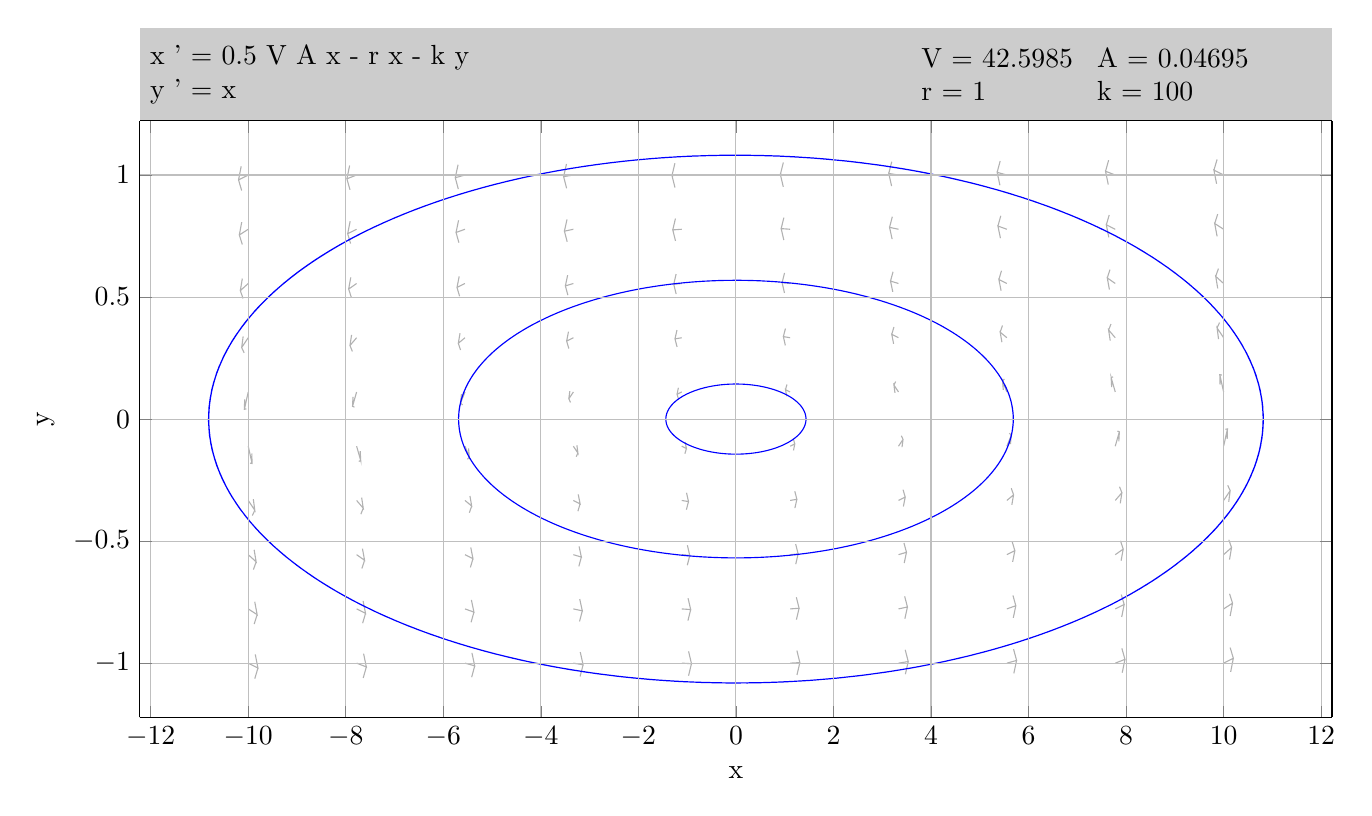
\begin{tikzpicture}

\begin{axis}[%
width=5.960653in,
height=0.465593in,
at={(0.602431in,3.953599in)},
scale only axis,
every outer x axis line/.append style={black},
every x tick label/.append style={font=\color{black}},
xmin=0,
xmax=1,
xtick={-1},
xticklabels={\empty},
every outer y axis line/.append style={black},
every y tick label/.append style={font=\color{black}},
ymin=0,
ymax=1,
ytick={-1},
yticklabels={\empty},
hide axis,
axis background/.style={fill=white!80!black},
axis x line*=bottom,
axis y line*=left
]
\node[right, align=left, inner sep=0mm, text=black]
at (axis cs:0.00806451612903225,0.495614035087719,0) {x ' = 0.5 V A x - r x - k y\\y ' = x};
\node[right, align=left, inner sep=0mm, text=black]
at (axis cs:0.80260034904014,0.5,0) {A = 0.04695\\k = 100};
\node[right, align=left, inner sep=0mm, text=black]
at (axis cs:0.655200698080279,0.5,0) {V = 42.5985\\r = 1};
\node[right, align=left, inner sep=0mm, text=black]
at (axis cs:0.624729493891798,0.5,0) { \\ };
\end{axis}

\begin{axis}[%
width=5.960653in,
height=2.982955in,
at={(0.602431in,0.970644in)},
scale only axis,
unbounded coords=jump,
separate axis lines,
every outer x axis line/.append style={black},
every x tick label/.append style={font=\color{black}},
xmin=-12.2222222222222,
xmax=12.2222222222222,
xlabel={x},
xmajorgrids,
every outer y axis line/.append style={black},
every y tick label/.append style={font=\color{black}},
ymin=-1.22222222222222,
ymax=1.22222222222222,
ylabel={y},
ymajorgrids,
every outer z axis line/.append style={black},
every z tick label/.append style={font=\color{black}},
zmin=-1,
zmax=1,
view={0}{90}
]
\addplot [color=white!70!black,solid,forget plot]
  table[row sep=crcr]{%
-10	-1\\
-9.80099256191613	-1.0199007433855\\
-9.85571960749492	-0.96417866084888\\
-9.80099256191613	-1.0199007433855\\
-9.86566997918767	-1.06368237989081\\
nan	0\\
-10	-0.777777777777778\\
-9.81737728682081	-0.801257840259308\\
-9.86629408515418	-0.748558143220051\\
-9.81737728682081	-0.801257840259308\\
-9.87803411639495	-0.839869499809646\\
nan	0\\
-10	-0.555555555555556\\
-9.83759367618969	-0.584788692723244\\
-9.87900728904086	-0.53541717062036\\
-9.83759367618969	-0.584788692723244\\
-9.89362385762471	-0.616620332525515\\
nan	0\\
-10	-0.333333333333333\\
-9.86547783233039	-0.37368998106148\\
-9.89574532069924	-0.327952444825634\\
-9.86547783233039	-0.37368998106148\\
-9.91592364456331	-0.395213528660438\\
nan	0\\
-10	-0.111111111111111\\
-9.92123448420009	-0.182000061773522\\
-9.92714190127446	-0.14104199762482\\
-9.92123448420009	-0.182000061773522\\
-9.96258637660566	-0.180424755524777\\
nan	0\\
-10	0.111111111111111\\
-10.0787654967689	0.0402221504615824\\
-10.0374136075759	0.0417974644642146\\
-10.0787654967689	0.0402221504615824\\
-10.0728580879006	0.0811802128486674\\
nan	0\\
-10	0.333333333333333\\
-10.1345221610083	0.292976682458109\\
-10.084076349987	0.271453137468603\\
-10.1345221610083	0.292976682458109\\
-10.1042546754246	0.338714217972749\\
nan	0\\
-10	0.555555555555555\\
-10.162406319409	0.526322416943766\\
-10.1063761389334	0.49449077867505\\
-10.162406319409	0.526322416943766\\
-10.1209927082393	0.575693938379555\\
nan	0\\
-10	0.777777777777778\\
-10.1826227097447	0.754297714454812\\
-10.1219658809905	0.715686056015536\\
-10.1826227097447	0.754297714454812\\
-10.133705912652	0.806997410887868\\
nan	0\\
-10	1\\
-10.1990074352088	0.980099256056232\\
-10.1343300186602	0.93631762043717\\
-10.1990074352088	0.980099256056232\\
-10.1442803906321	1.03582133804155\\
nan	0\\
-7.77777777777778	-1\\
-7.57851018865711	-1.01549859000878\\
-7.63441581789111	-0.961032115725981\\
-7.57851018865711	-1.01549859000878\\
-7.6421651128955	-1.06066591028632\\
nan	0\\
-7.77777777777778	-0.777777777777778\\
-7.59476230037469	-0.796079325129178\\
-7.64509155675777	-0.744834991572987\\
-7.59476230037469	-0.796079325129178\\
-7.65424233043347	-0.836342730274529\\
nan	0\\
-7.77777777777778	-0.555555555555556\\
-7.61469466554042	-0.578387190589545\\
-7.65791169045313	-0.530766922020008\\
-7.61469466554042	-0.578387190589545\\
-7.66932750797012	-0.612308478138688\\
nan	0\\
-7.77777777777778	-0.333333333333333\\
-7.64176027858743	-0.365070748237433\\
-7.67463117461851	-0.321545148968617\\
-7.64176027858743	-0.365070748237433\\
-7.69049988207056	-0.389553898563789\\
nan	0\\
-7.77777777777778	-0.111111111111111\\
-7.69373503706152	-0.169941020861541\\
-7.70424038183879	-0.131281362757348\\
-7.69373503706152	-0.169941020861541\\
-7.73365533671401	-0.173302733115476\\
nan	0\\
-7.77777777777778	0.111111111111111\\
-7.86182050467822	0.0522811935298542\\
-7.82190020721277	0.0489194870791218\\
-7.86182050467822	0.0522811935298542\\
-7.8513151660034	0.0909408505293409\\
nan	0\\
-7.77777777777778	0.333333333333333\\
-7.91379527200769	0.301595916439374\\
-7.86505566951522	0.277112767950085\\
-7.91379527200769	0.301595916439374\\
-7.8809243779622	0.345121515065039\\
nan	0\\
-7.77777777777778	0.555555555555555\\
-7.9408608866563	0.532723919633321\\
-7.88622804501219	0.49880263319036\\
-7.9408608866563	0.532723919633321\\
-7.8976438629733	0.580344187629622\\
nan	0\\
-7.77777777777778	0.777777777777778\\
-7.9607932525368	0.759476229912967\\
-7.90131322314289	0.719212825582654\\
-7.9607932525368	0.759476229912967\\
-7.9104639970753	0.810720562962167\\
nan	0\\
-7.77777777777778	1\\
-7.97704536467641	0.984501409651727\\
-7.91339044101975	0.939334090031551\\
-7.97704536467641	0.984501409651727\\
-7.92113973619389	1.03896788348087\\
nan	0\\
-5.55555555555556	-1\\
-5.35609195769038	-1.01108131086169\\
-5.41316070933451	-0.957891018136889\\
-5.35609195769038	-1.01108131086169\\
-5.41870136476536	-1.05762281706947\\
nan	0\\
-5.55555555555556	-0.777777777777778\\
-5.37224327611035	-0.79087151182512\\
-5.42396352643208	-0.741115321749616\\
-5.37224327611035	-0.79087151182512\\
-5.43051039345575	-0.832771461472218\\
nan	0\\
-5.55555555555556	-0.555555555555556\\
-5.39195737332755	-0.57191537343071\\
-5.43694687352717	-0.526107882511163\\
-5.39195737332755	-0.57191537343071\\
-5.44512678246474	-0.607906973625164\\
nan	0\\
-5.55555555555556	-0.333333333333333\\
-5.41837171942604	-0.35619730521182\\
-5.45381087729527	-0.315042154615895\\
-5.41837171942604	-0.35619730521182\\
-5.46524286323452	-0.383634072680653\\
nan	0\\
-5.55555555555556	-0.111111111111111\\
-5.46644572639698	-0.155666020956441\\
-5.48203994768322	-0.120022090713198\\
-5.46644572639698	-0.155666020956441\\
-5.50431740260588	-0.164577005292487\\
nan	0\\
-5.55555555555556	0.111111111111111\\
-5.64466537587741	0.0665561962162243\\
-5.60679370105713	0.0576452156042268\\
-5.64466537587741	0.0665561962162243\\
-5.62907115850458	0.102200125765154\\
nan	0\\
-5.55555555555556	0.333333333333333\\
-5.69273938827092	0.31046936040434\\
-5.64586824522406	0.283032594104196\\
-5.69273938827092	0.31046936040434\\
-5.65730023168856	0.35162451046188\\
nan	0\\
-5.55555555555556	0.555555555555555\\
-5.71915373542002	0.539195737221462\\
-5.66598432687716	0.503204137755573\\
-5.71915373542002	0.539195737221462\\
-5.67416423604421	0.585003227687807\\
nan	0\\
-5.55555555555556	0.777777777777778\\
-5.73886783312698	0.764684043466789\\
-5.68060071627781	0.722784094367228\\
-5.73886783312698	0.764684043466789\\
-5.6871475834333	0.814440233152942\\
nan	0\\
-5.55555555555556	1\\
-5.75501915184121	0.98891868896442\\
-5.69240974519662	0.942377183203679\\
-5.75501915184121	0.98891868896442\\
-5.69795040071441	1.04210898134651\\
nan	0\\
-3.33333333333333	-1\\
-3.13373863368348	-1.00665315660787\\
-3.19195375442647	-0.954758534713045\\
-3.13373863368348	-1.00665315660787\\
-3.1952803327304	-1.05455588453797\\
nan	0\\
-3.33333333333333	-0.777777777777778\\
-3.14982211247942	-0.785642544314177\\
-3.20290928710149	-0.737405309139779\\
-3.14982211247942	-0.785642544314177\\
-3.20684167036969	-0.829160919566735\\
nan	0\\
-3.33333333333333	-0.555555555555556\\
-3.16938813067322	-0.565392267589744\\
-3.2161125134627	-0.521454953314459\\
-3.16938813067322	-0.565392267589744\\
-3.2210308694798	-0.603427554644517\\
nan	0\\
-3.33333333333333	-0.333333333333333\\
-3.19534928245825	-0.347131738127626\\
-3.2332948965222	-0.308496203970567\\
-3.19534928245825	-0.347131738127626\\
-3.24019409891935	-0.37748822940811\\
nan	0\\
-3.33333333333333	-0.111111111111111\\
-3.24006087172952	-0.139092847808418\\
-3.26104717603634	-0.107380211398274\\
-3.24006087172952	-0.139092847808418\\
-3.27503804438499	-0.154016442200179\\
nan	0\\
-3.33333333333333	0.111111111111111\\
-3.42660579031844	0.0831293722317417\\
-3.39162861850307	0.0682057796492746\\
-3.42660579031844	0.0831293722317417\\
-3.40561948794275	0.114842008141831\\
nan	0\\
-3.33333333333333	0.333333333333333\\
-3.47131738221494	0.319534928151957\\
-3.42647256625511	0.289178437485969\\
-3.47131738221494	0.319534928151957\\
-3.4333717688458	0.358170461926771\\
nan	0\\
-3.33333333333333	0.555555555555555\\
-3.49727853458992	0.545718843354742\\
-3.44563579616274	0.50768355670084\\
-3.49727853458992	0.545718843354742\\
-3.45055415226315	0.589656157329132\\
nan	0\\
-3.33333333333333	0.777777777777778\\
-3.51684455306898	0.769913011146053\\
-3.45982499549036	0.726394636201657\\
-3.51684455306898	0.769913011146053\\
-3.46375737880622	0.818150246069483\\
nan	0\\
-3.33333333333333	1\\
-3.53292803203856	0.993346843329366\\
-3.47138633325934	0.945444115654249\\
-3.53292803203856	0.993346843329366\\
-3.47471291159465	1.04524146500686\\
nan	0\\
-1.11111111111111	-1\\
-0.911450731314515	-1.00221844865917\\
-0.970794233088701	-0.951637819112269\\
-0.911450731314515	-1.00221844865917\\
-0.971903457418286	-1.05146800901057\\
nan	0\\
-1.11111111111111	-0.777777777777778\\
-0.927500095235737	-0.78040079228232\\
-0.981927646372213	-0.733711133962114\\
-0.927500095235737	-0.78040079228232\\
-0.983239153624484	-0.825516641899801\\
nan	0\\
-1.11111111111111	-0.555555555555556\\
-0.946991290013525	-0.558837951963557\\
-0.9954066372408	-0.51682327776676\\
-0.946991290013525	-0.558837951963557\\
-0.997047835444801	-0.598883188315553\\
nan	0\\
-1.11111111111111	-0.333333333333333\\
-0.972719875808257	-0.337946374477419\\
-1.01308398611309	-0.30196465330848\\
-0.972719875808257	-0.337946374477419\\
-1.01539050668513	-0.371160270959907\\
nan	0\\
-1.11111111111111	-0.111111111111111\\
-1.0154383137563	-0.120678390643288\\
-1.0417483330797	-0.0938900074449316\\
-1.0154383137563	-0.120678390643288\\
-1.04653197284579	-0.141726406122338\\
nan	0\\
-1.11111111111111	0.111111111111111\\
-1.20678390708372	0.101543831310546\\
-1.1756902483418	0.080495816257563\\
-1.20678390708372	0.101543831310546\\
-1.18047388824208	0.128332214243867\\
nan	0\\
-1.11111111111111	0.333333333333333\\
-1.249502345759	0.328720292145728\\
-1.20683171506773	0.295506395840037\\
-1.249502345759	0.328720292145728\\
-1.20913823566153	0.364702013163982\\
nan	0\\
-1.11111111111111	0.555555555555555\\
-1.27523093174332	0.552273159128961\\
-1.22517438644701	0.512227922898887\\
-1.27523093174332	0.552273159128961\\
-1.2268155846603	0.594287833214991\\
nan	0\\
-1.11111111111111	0.777777777777778\\
-1.29472212661474	0.77515476326262\\
-1.23898306833486	0.73003891374126\\
-1.29472212661474	0.77515476326262\\
-1.24029457559244	0.821844421493075\\
nan	0\\
-1.11111111111111	1\\
-1.31077149059335	0.997781551333848\\
-1.25031876458214	0.948531991063134\\
-1.31077149059335	0.997781551333848\\
-1.25142798891522	1.04836218080425\\
nan	0\\
1.11111111111111	-1\\
1.31077149059335	-0.997781551333848\\
1.25031876458214	-0.948531991063134\\
1.31077149059335	-0.997781551333848\\
1.25142798891522	-1.04836218080425\\
nan	0\\
1.11111111111111	-0.777777777777778\\
1.29472212661474	-0.77515476326262\\
1.23898306833486	-0.73003891374126\\
1.29472212661474	-0.77515476326262\\
1.24029457559244	-0.821844421493075\\
nan	0\\
1.11111111111111	-0.555555555555556\\
1.27523093174332	-0.552273159128961\\
1.22517438644701	-0.512227922898888\\
1.27523093174332	-0.552273159128961\\
1.2268155846603	-0.594287833214991\\
nan	0\\
1.11111111111111	-0.333333333333333\\
1.249502345759	-0.328720292145728\\
1.20683171506773	-0.295506395840037\\
1.249502345759	-0.328720292145728\\
1.20913823566153	-0.364702013163982\\
nan	0\\
1.11111111111111	-0.111111111111111\\
1.20678390708372	-0.101543831310546\\
1.1756902483418	-0.080495816257563\\
1.20678390708372	-0.101543831310546\\
1.18047388824208	-0.128332214243867\\
nan	0\\
1.11111111111111	0.111111111111111\\
1.0154383137563	0.120678390643288\\
1.0417483330797	0.0938900074449316\\
1.0154383137563	0.120678390643288\\
1.04653197284579	0.141726406122338\\
nan	0\\
1.11111111111111	0.333333333333333\\
0.972719875808257	0.337946374477419\\
1.01308398611309	0.30196465330848\\
0.972719875808257	0.337946374477419\\
1.01539050668513	0.371160270959907\\
nan	0\\
1.11111111111111	0.555555555555555\\
0.946991290013525	0.558837951963557\\
0.9954066372408	0.51682327776676\\
0.946991290013525	0.558837951963557\\
0.997047835444801	0.598883188315553\\
nan	0\\
1.11111111111111	0.777777777777778\\
0.927500095235737	0.78040079228232\\
0.981927646372213	0.733711133962114\\
0.927500095235737	0.78040079228232\\
0.983239153624484	0.825516641899801\\
nan	0\\
1.11111111111111	1\\
0.911450731314515	1.00221844865917\\
0.970794233088701	0.951637819112269\\
0.911450731314515	1.00221844865917\\
0.971903457418286	1.05146800901057\\
nan	0\\
3.33333333333333	-1\\
3.53292803203856	-0.993346843329366\\
3.47138633325934	-0.945444115654249\\
3.53292803203856	-0.993346843329366\\
3.47471291159465	-1.04524146500686\\
nan	0\\
3.33333333333333	-0.777777777777778\\
3.51684455306899	-0.769913011146053\\
3.45982499549036	-0.726394636201657\\
3.51684455306899	-0.769913011146053\\
3.46375737880622	-0.818150246069483\\
nan	0\\
3.33333333333333	-0.555555555555556\\
3.49727853458992	-0.545718843354742\\
3.44563579616274	-0.50768355670084\\
3.49727853458992	-0.545718843354742\\
3.45055415226315	-0.589656157329132\\
nan	0\\
3.33333333333333	-0.333333333333333\\
3.47131738221494	-0.319534928151957\\
3.42647256625511	-0.289178437485969\\
3.47131738221494	-0.319534928151957\\
3.4333717688458	-0.358170461926771\\
nan	0\\
3.33333333333333	-0.111111111111111\\
3.42660579031845	-0.0831293722317417\\
3.39162861850307	-0.0682057796492746\\
3.42660579031845	-0.0831293722317417\\
3.40561948794275	-0.114842008141831\\
nan	0\\
3.33333333333333	0.111111111111111\\
3.24006087172952	0.139092847808418\\
3.26104717603634	0.107380211398274\\
3.24006087172952	0.139092847808418\\
3.27503804438499	0.154016442200179\\
nan	0\\
3.33333333333333	0.333333333333333\\
3.19534928245825	0.347131738127626\\
3.2332948965222	0.308496203970567\\
3.19534928245825	0.347131738127626\\
3.24019409891935	0.377488229408109\\
nan	0\\
3.33333333333333	0.555555555555555\\
3.16938813067322	0.565392267589744\\
3.21611251346271	0.521454953314459\\
3.16938813067322	0.565392267589744\\
3.2210308694798	0.603427554644517\\
nan	0\\
3.33333333333333	0.777777777777778\\
3.14982211247942	0.785642544314177\\
3.2029092871015	0.737405309139779\\
3.14982211247942	0.785642544314177\\
3.2068416703697	0.829160919566735\\
nan	0\\
3.33333333333333	1\\
3.13373863368348	1.00665315660787\\
3.19195375442647	0.954758534713045\\
3.13373863368348	1.00665315660787\\
3.1952803327304	1.05455588453797\\
nan	0\\
5.55555555555556	-1\\
5.75501915184122	-0.98891868896442\\
5.69240974519662	-0.942377183203679\\
5.75501915184122	-0.98891868896442\\
5.69795040071441	-1.04210898134651\\
nan	0\\
5.55555555555556	-0.777777777777778\\
5.73886783312699	-0.764684043466789\\
5.68060071627781	-0.722784094367228\\
5.73886783312699	-0.764684043466789\\
5.6871475834333	-0.814440233152942\\
nan	0\\
5.55555555555556	-0.555555555555556\\
5.71915373542003	-0.539195737221463\\
5.66598432687716	-0.503204137755573\\
5.71915373542003	-0.539195737221463\\
5.67416423604421	-0.585003227687808\\
nan	0\\
5.55555555555556	-0.333333333333333\\
5.69273938827093	-0.31046936040434\\
5.64586824522407	-0.283032594104196\\
5.69273938827093	-0.31046936040434\\
5.65730023168856	-0.35162451046188\\
nan	0\\
5.55555555555556	-0.111111111111111\\
5.64466537587741	-0.0665561962162243\\
5.60679370105713	-0.0576452156042268\\
5.64466537587741	-0.0665561962162243\\
5.62907115850458	-0.102200125765154\\
nan	0\\
5.55555555555556	0.111111111111111\\
5.46644572639698	0.155666020956441\\
5.48203994768322	0.120022090713198\\
5.46644572639698	0.155666020956441\\
5.50431740260589	0.164577005292487\\
nan	0\\
5.55555555555556	0.333333333333333\\
5.41837171942604	0.35619730521182\\
5.45381087729527	0.315042154615895\\
5.41837171942604	0.35619730521182\\
5.46524286323452	0.383634072680653\\
nan	0\\
5.55555555555556	0.555555555555555\\
5.39195737332755	0.57191537343071\\
5.43694687352717	0.526107882511162\\
5.39195737332755	0.57191537343071\\
5.44512678246474	0.607906973625164\\
nan	0\\
5.55555555555556	0.777777777777778\\
5.37224327611035	0.79087151182512\\
5.42396352643208	0.741115321749616\\
5.37224327611035	0.79087151182512\\
5.43051039345575	0.832771461472218\\
nan	0\\
5.55555555555556	1\\
5.35609195769039	1.01108131086169\\
5.41316070933452	0.957891018136889\\
5.35609195769039	1.01108131086169\\
5.41870136476536	1.05762281706947\\
nan	0\\
7.77777777777778	-1\\
7.97704536467641	-0.984501409651727\\
7.91339044101975	-0.939334090031551\\
7.97704536467641	-0.984501409651727\\
7.92113973619389	-1.03896788348087\\
nan	0\\
7.77777777777778	-0.777777777777778\\
7.9607932525368	-0.759476229912967\\
7.90131322314289	-0.719212825582655\\
7.9607932525368	-0.759476229912967\\
7.9104639970753	-0.810720562962167\\
nan	0\\
7.77777777777778	-0.555555555555556\\
7.9408608866563	-0.532723919633321\\
7.88622804501219	-0.49880263319036\\
7.9408608866563	-0.532723919633321\\
7.8976438629733	-0.580344187629622\\
nan	0\\
7.77777777777778	-0.333333333333333\\
7.91379527200769	-0.301595916439374\\
7.86505566951523	-0.277112767950085\\
7.91379527200769	-0.301595916439374\\
7.8809243779622	-0.345121515065039\\
nan	0\\
7.77777777777778	-0.111111111111111\\
7.86182050467822	-0.0522811935298542\\
7.82190020721277	-0.0489194870791218\\
7.86182050467822	-0.0522811935298542\\
7.8513151660034	-0.0909408505293408\\
nan	0\\
7.77777777777778	0.111111111111111\\
7.69373503706152	0.169941020861541\\
7.70424038183879	0.131281362757348\\
7.69373503706152	0.169941020861541\\
7.73365533671401	0.173302733115476\\
nan	0\\
7.77777777777778	0.333333333333333\\
7.64176027858744	0.365070748237433\\
7.67463117461851	0.321545148968617\\
7.64176027858744	0.365070748237433\\
7.69049988207056	0.389553898563789\\
nan	0\\
7.77777777777778	0.555555555555555\\
7.61469466554042	0.578387190589545\\
7.65791169045313	0.530766922020008\\
7.61469466554042	0.578387190589545\\
7.66932750797012	0.612308478138688\\
nan	0\\
7.77777777777778	0.777777777777778\\
7.59476230037469	0.796079325129178\\
7.64509155675777	0.744834991572987\\
7.59476230037469	0.796079325129178\\
7.65424233043347	0.836342730274529\\
nan	0\\
7.77777777777778	1\\
7.57851018865711	1.01549859000878\\
7.63441581789111	0.961032115725981\\
7.57851018865711	1.01549859000878\\
7.64216511289551	1.06066591028632\\
nan	0\\
10	-1\\
10.1990074352088	-0.980099256056232\\
10.1343300186602	-0.93631762043717\\
10.1990074352088	-0.980099256056232\\
10.1442803906321	-1.03582133804155\\
nan	0\\
10	-0.777777777777778\\
10.1826227097447	-0.754297714454812\\
10.1219658809905	-0.715686056015536\\
10.1826227097447	-0.754297714454812\\
10.133705912652	-0.806997410887868\\
nan	0\\
10	-0.555555555555556\\
10.162406319409	-0.526322416943766\\
10.1063761389334	-0.494490778675051\\
10.162406319409	-0.526322416943766\\
10.1209927082393	-0.575693938379556\\
nan	0\\
10	-0.333333333333333\\
10.1345221610083	-0.292976682458109\\
10.084076349987	-0.271453137468603\\
10.1345221610083	-0.292976682458109\\
10.1042546754246	-0.33871421797275\\
nan	0\\
10	-0.111111111111111\\
10.0787654967689	-0.0402221504615824\\
10.0374136075759	-0.0417974644642146\\
10.0787654967689	-0.0402221504615824\\
10.0728580879006	-0.0811802128486674\\
nan	0\\
10	0.111111111111111\\
9.92123448420009	0.182000061773522\\
9.92714190127446	0.14104199762482\\
9.92123448420009	0.182000061773522\\
9.96258637660566	0.180424755524777\\
nan	0\\
10	0.333333333333333\\
9.86547783233039	0.37368998106148\\
9.89574532069924	0.327952444825633\\
9.86547783233039	0.37368998106148\\
9.91592364456331	0.395213528660438\\
nan	0\\
10	0.555555555555555\\
9.83759367618969	0.584788692723244\\
9.87900728904086	0.53541717062036\\
9.83759367618969	0.584788692723244\\
9.89362385762471	0.616620332525514\\
nan	0\\
10	0.777777777777778\\
9.81737728682081	0.801257840259308\\
9.86629408515418	0.748558143220051\\
9.81737728682081	0.801257840259308\\
9.87803411639495	0.839869499809646\\
nan	0\\
10	1\\
9.80099256191613	1.0199007433855\\
9.85571960749492	0.96417866084888\\
9.80099256191613	1.0199007433855\\
9.86566997918767	1.06368237989081\\
nan	0\\
};
\addplot3 [color=blue,solid]
 table[row sep=crcr] {%
-1.08974358974359	0.0936895083236551	0\\
-1.11094845764074	0.0911650716500949	0.00229411764705883\\
-1.1315686834306	0.0885926553780006	0.00458823529411766\\
-1.151593377016	0.0859736167646501	0.00688235294117648\\
-1.17101198434257	0.0833093352465183	0.00917647058823531\\
-1.18981428739878	0.0806012124392779	0.0114705882352941\\
-1.20799040421588	0.0778506721377989	0.013764705882353\\
-1.22553078886793	0.0750591603161489	0.0160588235294118\\
-1.24242623147182	0.0722281451275926	0.0183529411764706\\
-1.28565917727259	0.0642184926821751	0.0246870334370418\\
-1.32373979303399	0.0559510217925656	0.0310211256976129\\
-1.35650902570524	0.0474594168439177	0.0373552179581841\\
-1.38383230745284	0.0387778713500216	0.0436893102187552\\
-1.40559955566063	0.0299410879533043	0.0500234024793264\\
-1.42172517292975	0.0209842784248295	0.0563574947398975\\
-1.43214804707867	0.0119431636642975	0.0626915870004687\\
-1.43683155114318	0.00285397370004542	0.0690256792610398\\
-1.43629846781184	-0.0048465587739312	0.074384586545643\\
-1.43164249215365	-0.0125333615410393	0.0797434938302461\\
-1.42287588717471	-0.0201840255456471	0.0851024011148492\\
-1.41002305224865	-0.0277764640362485	0.0904613083994524\\
-1.39312052311661	-0.0352889125654636	0.0958202156840555\\
-1.37221697188727	-0.0426999289900381	0.101179122968659\\
-1.34737320703685	-0.0499883934708437	0.106538030253262\\
-1.31866217340906	-0.0571335084728779	0.111896937537865\\
-1.28936693125971	-0.0634687454496803	0.116754105230072\\
-1.25703036769481	-0.0696543995675498	0.12161127292228\\
-1.22172906651389	-0.0756756641203108	0.126468440614487\\
-1.18354621552589	-0.081518250529489	0.131325608306695\\
-1.14257160654911	-0.0871683883443108	0.136182775998902\\
-1.09890163541126	-0.0926128252417039	0.141039943691109\\
-1.05263930194942	-0.0978388270262966	0.145897111383317\\
-1.00389421001005	-0.102834177630419	0.150754279075524\\
-0.94147449381256	-0.108578134752906	0.156657395237315\\
-0.875773872526712	-0.113944158661805	0.162560511399106\\
-0.807023853839124	-0.118913040603698	0.168463627560898\\
-0.735464411157682	-0.123467238527721	0.174366743722689\\
-0.661343983611549	-0.127590877085559	0.18026985988448\\
-0.584919476051158	-0.13126974763145	0.186172976046271\\
-0.506456259048213	-0.134491308222181	0.192076092208062\\
-0.426228168895693	-0.137244683617092	0.197979208369853\\
-0.337369120513804	-0.139695061085249	0.204393822948018\\
-0.247118750915005	-0.141571196495501	0.210808437526182\\
-0.155855227241736	-0.142864838401654	0.217223052104347\\
-0.0639560900455617	-0.143570369714398	0.223637666682511\\
0.0282017467128193	-0.143684807701311	0.230052281260676\\
0.120241995663581	-0.143207803986853	0.23646689583884\\
0.211788996027767	-0.142141644552375	0.242881510417005\\
0.302467713617294	-0.140491249736109	0.249296124995169\\
0.374530326706228	-0.13874419256146	0.25445623346762\\
0.445597564294319	-0.136627819072488	0.25961634194007\\
0.515477291178501	-0.134147742116582	0.26477645041252\\
0.583982361341667	-0.131310527114421	0.26993655888497\\
0.650930617952667	-0.128123692059972	0.27509666735742\\
0.716144893366311	-0.124595707520488	0.28025677582987\\
0.779453009123367	-0.120735996636512	0.28541688430232\\
0.840687775950561	-0.116554935121875	0.290576992774771\\
0.903379555984071	-0.111766265895621	0.296066885022694\\
0.963351601175839	-0.106640784375539	0.301556777270618\\
1.02041938835481	-0.101194062027148	0.307046669518541\\
1.07440934328257	-0.0954425211690875	0.312536561766465\\
1.12515884065335	-0.0894034349731199	0.318026454014388\\
1.17251620409404	-0.0830949274641299	0.323516346262312\\
1.21634070616417	-0.076535973520124	0.329006238510235\\
1.2565025683559	-0.0697463988722309	0.334496130758159\\
1.29802789404237	-0.0616754202262133	0.340812656561782\\
1.33437999599824	-0.0533581875589693	0.347129182365405\\
1.36540775771117	-0.0448284057808007	0.353445708169028\\
1.39098435966454	-0.0361202367221496	0.359762233972652\\
1.41100727933743	-0.0272682991335985	0.366078759776275\\
1.42539829120465	-0.01830766868587	0.372395285579898\\
1.4341034667367	-0.00927387796982706	0.378711811383521\\
1.43709317439981	-0.00020291649647268	0.385028337187144\\
1.43520807027592	0.00736288577610399	0.39029505708023\\
1.42934360734208	0.0149084407893252	0.395561776973316\\
1.41951510973289	0.02241250965937	0.400828496866402\\
1.40574915958086	0.0298541697603562	0.406095216759488\\
1.38808359701638	0.0372128147243405	0.411361936652573\\
1.3665675201677	0.0444681544413185	0.416628656545659\\
1.34126128516099	0.0516002150592245	0.421895376438745\\
1.31223650612028	0.0585893389839319	0.427162096331831\\
1.28238785646704	0.0648628242680889	0.431996779578547\\
1.24954226701308	0.0709848483804904	0.436831462825262\\
1.21377682569007	0.0769408934046716	0.441666146071978\\
1.17517504896837	0.0827169562748799	0.446500829318694\\
1.13382688185704	0.0882995487760752	0.451335512565409\\
1.08982869790384	0.0936756975439296	0.456170195812125\\
1.04328329919522	0.0988329440648275	0.461004879058841\\
0.994299916356322	0.103759344675866	0.465839562305556\\
0.931120998696761	0.109464662799147	0.471763693677255\\
0.864674068620264	0.1147862451048	0.477687825048954\\
0.795194973550117	0.119704898431482	0.483611956420652\\
0.722927978903567	0.124203129554983	0.489536087792351\\
0.64812576809182	0.128265145188226	0.49546021916405\\
0.571049442520045	0.131876851981267	0.501384350535749\\
0.491968521587372	0.135025856521297	0.507308481907447\\
0.41116094268689	0.137701465332639	0.513232613279146\\
0.322567563129985	0.140042162345764	0.519609570909251\\
0.232659333233192	0.141813914837976	0.525986528539356\\
0.141808551494208	0.143009010373195	0.532363486169462\\
0.0503866631003236	0.143622306718884	0.538740443799567\\
-0.0412357400715705	0.143651231846051	0.545117401429672\\
-0.132688919454988	0.143095783929243	0.551494359059777\\
-0.223603989793844	0.141958531346555	0.557871316689882\\
-0.313612919142459	0.140244612679621	0.564248274319987\\
-0.385364891133967	0.138445089858782	0.569396206724845\\
-0.456097462593577	0.136278782003085	0.574544139129703\\
-0.525620309522583	0.133751410474954	0.57969207153456\\
-0.593748118504736	0.130869636342539	0.584840003939418\\
-0.660300586706244	0.127641060379717	0.589987936344275\\
-0.725102421875775	0.124074223066093	0.595135868749133\\
-0.787983342344451	0.120178604587001	0.600283801153991\\
-0.848778077025857	0.115964624833499	0.605431733558848\\
-0.911339855068811	0.111115552194872	0.610940168310828\\
-0.97113937356	0.105929360950634	0.616448603062807\\
-1.02799135324381	0.100421915666135	0.621957037814786\\
-1.08172168333337	0.0946099349420716	0.627465472566766\\
-1.13216742151055	0.0885109914144883	0.632973907318745\\
-1.17917679392597	0.0821435117547767	0.638482342070725\\
-1.22260919519898	0.0755267766696751	0.643990776822704\\
-1.26233518841769	0.0686809209012689	0.649499211574683\\
-1.3032500180052	0.0605593868731712	0.655827903345154\\
-1.33895077902356	0.0521951134677012	0.662156595115625\\
-1.36928838676096	0.0436221317072693	0.668485286886096\\
-1.39413828761038	0.0348749112272457	0.674813978656566\\
-1.41340045906957	0.0259883602759602	0.681142670427037\\
-1.42699940974102	0.0169978257147023	0.687471362197508\\
-1.43488417933201	0.00793909301772117	0.693800053967979\\
-1.43702833865459	-0.00115161372777448	0.700128745738449\\
-1.43443802911668	-0.00870234848217766	0.705386509767322\\
-1.42788398673295	-0.016229202626841	0.710644273796195\\
-1.4173834251142	-0.0237110617989856	0.715902037825068\\
-1.40296470860763	-0.0311271357594244	0.72115980185394\\
-1.38466735229688	-0.0384569583925616	0.726417565882813\\
-1.36254202200201	-0.0456803877063936	0.731675329911686\\
-1.3366505342795	-0.0527776058325078	0.736933093940559\\
-1.30706585642227	-0.0597291190260841	0.742190857969431\\
-1.27646636037893	-0.0660161425862018	0.747056760397047\\
-1.24284511131204	-0.0721470152311426	0.751922662824663\\
-1.20628205352591	-0.0781070061233329	0.756788565252279\\
-1.16686367711774	-0.0838819196839832	0.761654467679895\\
-1.12468301797762	-0.0894580955930878	0.766520370107511\\
-1.07983965778855	-0.0948224087894251	0.771386272535127\\
-1.03243972402641	-0.0999622694705572	0.776252174962743\\
-0.982595889959974	-0.10486562309283	0.781118077390359\\
-0.918577208272306	-0.110516770303078	0.787060780029799\\
-0.851314241027918	-0.11577806023865	0.793003482669239\\
-0.781047276639191	-0.120630390005449	0.798946185308679\\
-0.708024923450605	-0.125056388819186	0.804888887948119\\
-0.632504109738742	-0.129040418005384	0.810831590587559\\
-0.554750083712288	-0.132568570999371	0.816774293226999\\
-0.475036413512028	-0.135628673346288	0.822716995866439\\
-0.393644987210847	-0.138210282701081	0.828659698505879\\
-0.305397606660973	-0.140424515450453	0.83499147290556\\
-0.215922774355375	-0.142076289205264	0.84132324730524\\
-0.125585729756837	-0.143158501934426	0.84765502170492\\
-0.0347506136207802	-0.143666546208342	0.8539867961046\\
0.0562195320047367	-0.143598309198906	0.86031857050428\\
0.146962763779018	-0.142954172679502	0.866650344903961\\
0.237118237068731	-0.141737013025003	0.872982119303641\\
0.326326205947906	-0.139952201211775	0.879313893703321\\
0.397714116954802	-0.138093312237628	0.884447580175744\\
0.468055710379168	-0.135870589994097	0.889581266648166\\
0.537162766425856	-0.13328987586796	0.894714953120589\\
0.6048520973308	-0.130357936120167	0.899848639593012\\
0.670945547361018	-0.127082461885839	0.904982326065435\\
0.73526999281461	-0.123472069174266	0.910116012537857\\
0.797657342020756	-0.11953629886891	0.91524969901028\\
0.857944535339721	-0.115285616727403	0.920383385482703\\
0.920349407317701	-0.11036786179846	0.925912728751504\\
0.979943501806053	-0.105112708138858	0.931442072020304\\
1.03654072331413	-0.0995363559159953	0.936971415289105\\
1.08996639641742	-0.0936558626319588	0.942500758557906\\
1.14005726575752	-0.0874891431235225	0.948030101826707\\
1.18666149604217	-0.0810549695621478	0.953559445095507\\
1.22963867204523	-0.0743729714539833	0.959088788364308\\
1.26885979860669	-0.067463635639865	0.964618131633109\\
1.30907354592403	-0.0592851986169733	0.970960624506594\\
1.34402705253966	-0.0508680813735757	0.97730311738008\\
1.37357359626878	-0.0422466849720895	0.983645610253566\\
1.39759125155419	-0.0334558278280605	0.989988103127051\\
1.41598288946628	-0.024530745710163	0.996330596000537\\
1.42867617770299	-0.0155070917401999	1.00267308887402\\
1.43562358058985	-0.00642093639310301	1.00901558174751\\
1.43680235907997	0.00269123250306778	1.01535807462099\\
1.43340667354476	0.0102338016842819	1.02061245485596\\
1.4260551809151	0.0177482942739739	1.02586683509092\\
1.41476730948986	0.0252136568360379	1.03112121532589\\
1.39957357398021	0.0326091709257238	1.03637559556085\\
1.38051557550961	0.0399144530896379	1.04162997579582\\
1.35764600161383	0.0471094548657424	1.04688435603078\\
1.33102862624092	0.0541744627833557	1.05213873626575\\
1.30073830975128	0.0610900983631523	1.05739311650071\\
1.26919838355199	0.0673986103091079	1.06230145733183\\
1.23460127133002	0.0735449097144884	1.06720979816295\\
1.19703069603582	0.079513965040977	1.07211813899406\\
1.15657709356454	0.0852913077387415	1.07702647982518\\
1.11333761275604	0.0908630322464345	1.0819348206563\\
1.0674161153949	0.0962157959911931	1.08684316148741\\
1.01892317621039	0.101336819388639	1.09175150231853\\
0.967976082876528	0.106213885842879	1.09665984314964\\
0.90293414753719	0.111795879131656	1.10262474931555\\
0.834679232109693	0.116980549938762	1.10858965548145\\
0.763457050821037	0.121748922619779	1.11455456164735\\
0.689521505621789	0.126083792768729	1.12051946781325\\
0.613134686186076	0.129969727218072	1.12648437397916\\
0.534566869911592	0.133393064038708	1.13244928014506\\
0.454096521919594	0.136341912539976	1.13841418631096\\
0.3720102950549	0.138806153269654	1.14437909247686\\
0.2842147741488	0.140866447489543	1.15065511635394\\
0.195296755640558	0.142372384886981	1.15693114023101\\
0.10561280040547	0.143317586555508	1.16320716410808\\
0.0155180902656005	0.143698076927377	1.16948318798515\\
-0.074633572010212	0.14351228377356	1.17575921186223\\
-0.164489762706356	0.142761038203745	1.1820352357393\\
-0.253699437160447	0.141447574666333	1.18831125961637\\
-0.34191292976333	0.139577530948445	1.19458728349344\\
-0.412848843698202	0.137646326040253	1.19970359417766\\
-0.4827058868163	0.135354913595005	1.20481990486187\\
-0.551298406393802	0.132709278888484	1.20993621554608\\
-0.618445806454726	0.129716314108008	1.2150525262303\\
-0.683972547770927	0.126383818352423	1.22016883691451\\
-0.747708147862096	0.122720497632109	1.22528514759872\\
-0.809487180995759	0.118735964868977	1.23040145828294\\
-0.869149278187285	0.114440739896469	1.23551776896715\\
-0.931347620488591	0.109438741797198	1.24107246193665\\
-0.990675464605378	0.104099108407628	1.24662715490614\\
-1.04694578362812	0.0984384545907662	1.25218184787564\\
-1.0999832817817	0.0924742560837746	1.25773654084514\\
-1.14962439442543	0.086224849497967	1.26329123381464\\
-1.19571728805306	0.0797094323188109	1.26884592678414\\
-1.23812186029274	0.0729480629059273	1.27440061975363\\
-1.27670973990704	0.06596166049309	1.27995531272313\\
-1.31605328725445	0.0577142371446977	1.28631470534074\\
-1.35008032079184	0.0492332048601571	1.29267409795834\\
-1.3786470928006	0.0405534177606518	1.29903349057595\\
-1.4016349771343	0.0317101205868326	1.30539288319355\\
-1.41895046921866	0.0227389486988172	1.31175227581116\\
-1.43052518605161	0.0136759280761904	1.31811166842877\\
-1.43631586620323	0.00455747531800394	1.32447106104637\\
-1.43630436981578	-0.00457960235722348	1.33083045366398\\
-1.43192255071888	-0.0121110630433026	1.33608072275805\\
-1.42359517631691	-0.019609318012753	1.34133099185212\\
-1.41134437761197	-0.0270533911134813	1.34658126094619\\
-1.39520329212904	-0.0344226543980808	1.35183153004026\\
-1.37521606391595	-0.0416968281238309	1.35708179913434\\
-1.35143784354343	-0.048855980752698	1.36233206822841\\
-1.32393478810506	-0.0558805289513347	1.36758233732248\\
-1.2927840612173	-0.0627512375910801	1.37283260641655\\
-1.26009354636234	-0.0690817204366282	1.37779092782749\\
-1.22430564475509	-0.0752425381573852	1.38274924923843\\
-1.18550875576729	-0.0812183092026787	1.38770757064938\\
-1.14379818609725	-0.0869942493575483	1.39266589206032\\
-1.09927614976993	-0.0925561717427457	1.39762421347126\\
-1.05205176813688	-0.0978904868147344	1.4025825348822\\
-1.00224106987626	-0.10298420236569	1.40754085629314\\
-0.94996699099285	-0.1078249235235	1.41249917770409\\
-0.883693485655228	-0.11332034001994	1.41849083205136\\
-0.814247113136128	-0.118409395289414	1.42448248639862\\
-0.741880194631829	-0.123073283729121	1.43047414074589\\
-0.666853066160304	-0.127295018633495	1.43646579509316\\
-0.58943407856122	-0.131059432194207	1.44245744944043\\
-0.509899597495934	-0.134353175500165	1.4484491037877\\
-0.428534003447498	-0.137164718537513	1.45444075813497\\
-0.345629691720655	-0.139484350189633	1.46043241248224\\
-0.258419442866626	-0.141360333260458	1.46664063550684\\
-0.170210241865776	-0.142691947645894	1.47284885853143\\
-0.0813481527446412	-0.143473651243035	1.47905708155603\\
0.00782244929957621	-0.14370219729201	1.48526530458062\\
0.0969588778990065	-0.143376634375979	1.49147352760522\\
0.185720135515114	-0.142498306421139	1.49768175062981\\
0.273766913438697	-0.141070852696722	1.50388997365441\\
0.360761591789887	-0.139100207814991	1.510098196679\\
0.431142724611694	-0.137082227745252	1.51519364585571\\
0.500406261248863	-0.134708432583606	1.52028909503242\\
0.568369632952556	-0.131984976974723	1.52538454420913\\
0.634855355438203	-0.128918901084517	1.53047999338583\\
0.699691028885505	-0.125518130600142	1.53557544256254\\
0.76270933793843	-0.121791476729996	1.54067089173925\\
0.823748051705218	-0.117748636203718	1.54576634091596\\
0.882650023758377	-0.113400191272191	1.55086179009266\\
0.944577757915556	-0.10829625219106	1.55644675094418\\
1.00356241354773	-0.102854548559415	1.5620317117957\\
1.05941593932094	-0.0970922016129841	1.56761667264722\\
1.11196239513418	-0.0910271969914383	1.57320163349874\\
1.16103795211938	-0.0846783847383916	1.57878659435026\\
1.2064908926414	-0.0780654793014008	1.58437155520178\\
1.24818161029807	-0.0712090595319657	1.5899565160533\\
1.28598260992011	-0.0641305686855286	1.59554147690482\\
1.32425773040761	-0.0558008616906357	1.60192129014242\\
1.35714877246703	-0.0472438206080031	1.60830110338002\\
1.38451570235251	-0.0384948466195547	1.61468091661762\\
1.40624400002294	-0.0295896981913909	1.62106072985522\\
1.422244659142	-0.0205644910737884	1.62744054309282\\
1.43245418707813	-0.011455698301201	1.63382035633042\\
1.43683460490452	-0.00230015019225881	1.64020016956802\\
1.43537344739917	0.00686496565023159	1.64657998280562\\
1.42980062089623	0.0143813549488566	1.65182533039143\\
1.42029543797715	0.0218583563420295	1.65707067797724\\
1.4068832806742	0.0292750910362237	1.66231602556305\\
1.38960043934961	0.0366110442637491	1.66756137314886\\
1.36849411269555	0.0438460652827515	1.67280672073467\\
1.34362240773418	0.0509603673772134	1.67805206832048\\
1.3150543398176	0.0579345278569529	1.68329741590629\\
1.28286983262785	0.0647494880576249	1.6885427634921\\
};
 \addplot3 [color=blue,solid]
 table[row sep=crcr] {%
-4.12393162393162	0.391792489353465	0\\
-4.14760685201134	0.389285305490401	0.000606217616580311\\
-4.17112965618823	0.386763815434625	0.00121243523316062\\
-4.19449917181499	0.384228111869034	0.00181865284974093\\
-4.21771453999482	0.381678287986887	0.00242487046632124\\
-4.24077490758141	0.379114437491805	0.00303108808290156\\
-4.263679427179	0.376536654597774	0.00363730569948187\\
-4.28642725714228	0.373945034029139	0.00424352331606218\\
-4.30901756157648	0.37133967102061	0.00484974093264249\\
-4.4839763779758	0.350013246366952	0.00969948186528498\\
-4.64839526558659	0.327863528241062	0.0145492227979275\\
-4.8018804705711	0.304943082609273	0.01939896373057\\
-4.94406789392686	0.281305927114267	0.0242487046632124\\
-5.07462309148671	0.257007531075073	0.0290984455958549\\
-5.19324127391879	0.232104815487075	0.0339481865284974\\
-5.29964730672651	0.206656153022002	0.0387979274611399\\
-5.39359571024861	0.180721368027933	0.0436476683937824\\
-5.49544142558261	0.146871552007563	0.0498625578677034\\
-5.57608038183022	0.11245342423787	0.0560774473416243\\
-5.63518290172286	0.0776022074394753	0.0622923368155453\\
-5.67251081515407	0.0424531855358263	0.0685072262894662\\
-5.6879174591795	0.00714170365319811	0.0747221157633872\\
-5.68134767801691	-0.0281968318793068	0.0809370052373081\\
-5.65283782304618	-0.0634269535297585	0.0871518947112291\\
-5.6025157528093	-0.0984131325634007	0.09336678418515\\
-5.54486488688091	-0.126933193710453	0.0984824162053475\\
-5.47270787437356	-0.155121769006015	0.103598048225545\\
-5.38623230854108	-0.182903991781043	0.108713680245742\\
-5.28566290964119	-0.210206753517353	0.11382931226594\\
-5.1712615249355	-0.236958703847625	0.118944944286137\\
-5.04332712868948	-0.263090250555403	0.124060576306335\\
-4.9021958221725	-0.288533559575092	0.129176208326532\\
-4.7482408336578	-0.313222554991965	0.13429184034673\\
-4.57318725984229	-0.338269573344897	0.139664382554174\\
-4.38493537384147	-0.362341247164947	0.145036924761619\\
-4.1840324781992	-0.385366739905088	0.150409466969063\\
-3.9710585217838	-0.407279031606665	0.155782009176508\\
-3.74662609978804	-0.428014918899393	0.161154551383953\\
-3.51138045372921	-0.447515015001359	0.166527093591397\\
-3.26599947144904	-0.465723749719018	0.171899635798842\\
-3.01119368711372	-0.482589369447198	0.177272178006286\\
-2.70471257549889	-0.500411580303659	0.183505484986426\\
-2.38771700524895	-0.516291632764548	0.189738791966565\\
-2.06145685175693	-0.530165488270088	0.195972098946705\\
-1.72720405175161	-0.541978105217375	0.202205405926844\\
-1.38625260329749	-0.551683438960373	0.208438712906984\\
-1.03991856579482	-0.559244441809921	0.214672019887123\\
-0.68954005997956	-0.564633063033727	0.220905326867263\\
-0.336477267923401	-0.567830248856369	0.227138633847402\\
-0.0241283246757024	-0.568821629021962	0.232632988550483\\
0.288301570527475	-0.568096716419708	0.238127343253565\\
0.599854524071113	-0.565657132595176	0.243621697956646\\
0.909584999019631	-0.561509865514773	0.249116052659727\\
1.21655981511688	-0.555667269565747	0.254610407362808\\
1.51985814878616	-0.548147065556185	0.260104762065889\\
1.81857153313019	-0.538972340715011	0.26559911676897\\
2.11180385793114	-0.528171548691993	0.271093471472052\\
2.36652657963847	-0.517260191875492	0.275965436048032\\
2.6156381889965	-0.50512130778331	0.280837400624013\\
2.85853878420244	-0.491783802705582	0.285709365199994\\
3.09464848454916	-0.477279286287024	0.290581329775974\\
3.32340743042513	-0.461642071526931	0.295453294351955\\
3.54427578331448	-0.444909174779177	0.300325258927936\\
3.75673372579693	-0.427120315752213	0.305197223503916\\
3.96028146154785	-0.408317917509072	0.310069188079897\\
4.19167400658945	-0.384527281039016	0.315904148794706\\
4.40881120732118	-0.359427433092027	0.321739109509515\\
4.61093451853802	-0.333104742820725	0.327574070224324\\
4.797347286729	-0.3056489623124	0.333409030939133\\
4.96741475007718	-0.277153226589014	0.339243991653942\\
5.1205640384597	-0.2477140536072	0.345078952368751\\
5.25628417344774	-0.217431344258262	0.35091391308356\\
5.37412606830651	-0.186408382368176	0.356748873798369\\
5.46334560147278	-0.15836444103369	0.36192294418943\\
5.53794702248696	-0.129896136363105	0.367097014580491\\
5.59772378725259	-0.101080630291524	0.372271084971552\\
5.64251230340643	-0.0719953549398522	0.377445155362612\\
5.67219193031841	-0.0427180126147977	0.382619225753673\\
5.68668497909165	-0.0133265758088727	0.387793296144734\\
5.68595671256243	0.0161007127996075	0.392967366535795\\
5.67001534530024	0.0454853403465254	0.398141436926856\\
5.64078285809793	0.0733185156134468	0.40306183865363\\
5.59789816368588	0.100974718880506	0.407982240380404\\
5.54146332408324	0.128386100896195	0.412902642107177\\
5.47161343219913	0.15548597862435	0.417823043833951\\
5.38851661183268	0.182208835244146	0.422743445560725\\
5.292374017673	0.208490320150103	0.427663847287498\\
5.18341983529918	0.23426724895208	0.432584249014272\\
5.0619212811803	0.259477603475279	0.437504650741046\\
4.92406251233087	0.284772701551832	0.44256951920658\\
4.77357432840155	0.309338036039669	0.447634387672115\\
4.61084476383835	0.333109557415416	0.45269925613765\\
4.43629098144472	0.356025874386576	0.457764124603185\\
4.25035927238155	0.378028253891523	0.46282899306872\\
4.05352505616721	0.399060621099506	0.467893861534255\\
3.84629288067752	0.419069559410648	0.47295872999979\\
3.62919642214573	0.438004310455945	0.478023598465324\\
3.35878260667914	0.459069838953887	0.484050341366114\\
3.07616689651793	0.478469811095947	0.490077084266904\\
2.78238867436753	0.496131614402168	0.496103827167694\\
2.47851746007726	0.511990111365226	0.502130570068484\\
2.16565291064033	0.525987639450428	0.508157312969274\\
1.84492482019383	0.538074011095716	0.514184055870064\\
1.51749312001873	0.548206513711663	0.520210798770854\\
1.18454787853987	0.556349909681473	0.526237541671644\\
0.844768217772451	0.562513418333195	0.53230901405864\\
0.501863496617625	0.566604948490485	0.538380486445636\\
0.157119896572411	0.568608056089397	0.544451958832632\\
-0.188184762729575	0.568514564300615	0.550523431219629\\
-0.532781023518129	0.566324563529453	0.556594903606625\\
-0.875407789886455	0.562046411415861	0.562666375993621\\
-1.21481232779117	0.555696732834419	0.568737848380617\\
-1.54975026505229	0.547300419894337	0.574809320767614\\
-1.82324828530566	0.538806983589037	0.579844401606813\\
-2.09213081923931	0.528947919482266	0.584879482446012\\
-2.35570598703432	0.51774821647082	0.589914563285211\\
-2.61330171973384	0.505236163822732	0.59494964412441\\
-2.86426575924312	0.491443351177273	0.599984724963609\\
-3.10796565832948	0.476404668544946	0.605019805802808\\
-3.34378878062231	0.460158306307494	0.610054886642008\\
-3.57114230061313	0.442745755217895	0.615089967481207\\
-3.81415779145957	0.421991657664949	0.620708736873085\\
-4.04514495534751	0.399905411307678	0.626327506264964\\
-4.26335805365764	0.376557371227669	0.631946275656843\\
-4.46810114484899	0.35202130688975	0.637565045048721\\
-4.65872808445894	0.326374402141983	0.6431838144406\\
-4.8346425251032	0.299697255215671	0.648802583832479\\
-4.99529791647582	0.272073878725352	0.654421353224357\\
-5.1401975053492	0.2435916996688	0.660040122616236\\
-5.28550287560917	0.210211977125492	0.666440928369601\\
-5.40917701232602	0.175970104149168	0.672841734122965\\
-5.51068886772566	0.141008719814198	0.67924253987633\\
-5.58961004534277	0.10547168238293	0.685643345629694\\
-5.64561480002086	0.0695040693056884	0.692044151383059\\
-5.67848003791218	0.0332521772207712	0.698444957136423\\
-5.68808531647779	-0.00313647804554534	0.704845762889788\\
-5.67441284448756	-0.0395131614790109	0.711246568643153\\
-5.64609928259908	-0.0690427418994322	0.716462220061253\\
-5.602432440909	-0.0983852126178723	0.721677871479354\\
-5.5435284203783	-0.127459566099091	0.726893522897454\\
-5.46954521113571	-0.15618628824955	0.732109174315555\\
-5.38068269247762	-0.184487358417413	0.737324825733656\\
-5.27718263286816	-0.212286249392543	0.742540477151756\\
-5.15932868993917	-0.239507927406507	0.747756128569857\\
-5.02744641049016	-0.266078852132574	0.752971779987957\\
-4.88619334767184	-0.291207120609591	0.758039957992285\\
-4.73239153571431	-0.315588148071319	0.763108135996613\\
-4.56643816519538	-0.33915827533358	0.768176314000941\\
-4.38875927711114	-0.361856546976272	0.773244492005268\\
-4.19980976287587	-0.38362471134337	0.778312670009596\\
-4.00007336432216	-0.404407220542926	0.783380848013924\\
-3.79006267370079	-0.424151230447069	0.788449026018252\\
-3.57031913368082	-0.442806600692004	0.793517204022579\\
-3.2959746911362	-0.463590210496098	0.799568639544987\\
-3.0095578868695	-0.482678054100228	0.805620075067395\\
-2.71213097773892	-0.499998054981727	0.811671510589803\\
-2.40478577190435	-0.515485782076448	0.817722946112212\\
-2.08864362882742	-0.529084449778774	0.82377438163462\\
-1.76485545927145	-0.540744917941607	0.829825817157028\\
-1.43460172530147	-0.550425691876374	0.835877252679436\\
-1.09909244028423	-0.558092922353029	0.841928688201844\\
-0.761516157928829	-0.563692784185175	0.847945116410049\\
-0.421172622735836	-0.567253738481377	0.853961544618254\\
-0.0793151826690086	-0.56876163394853	0.859977972826459\\
0.262811901477497	-0.568210270258581	0.865994401034665\\
0.60397345607912	-0.565601398048532	0.87201082924287\\
0.942943394680898	-0.560944718920441	0.878027257451075\\
1.27850471799746	-0.554257885441417	0.88404368565928\\
1.60944951391305	-0.545566501143626	0.890060113867485\\
1.88111327690057	-0.536805837610547	0.895078693133917\\
2.14804599031558	-0.52669351230353	0.900097272400348\\
2.40956531211415	-0.515255000443775	0.905115851666779\\
2.66500877638157	-0.502519013473205	0.91013443093321\\
2.91373379333236	-0.488517499054469	0.915153010199642\\
3.15511764931028	-0.473285641070941	0.920171589466073\\
3.3885575067883	-0.456861859626723	0.925190168732504\\
3.61347040436866	-0.439287811046638	0.930208747998936\\
3.85547012426775	-0.418209946301757	0.935851251725843\\
4.08520833081706	-0.395800683243594	0.94149375545275\\
4.30193679065849	-0.372132022881153	0.947136259179657\\
4.50495830517692	-0.347279386110693	0.952778762906564\\
4.69362671050019	-0.321321613715726	0.958421266633471\\
4.86734687749908	-0.29434096636702	0.964063770360378\\
5.02557471178736	-0.266423124622595	0.969706274087286\\
5.16781715372172	-0.237657188927728	0.975348777814193\\
5.30960498081552	-0.204025761674569	0.981765996666068\\
5.42955132166862	-0.169553198082989	0.988183215517944\\
5.52713781718929	-0.134383863691685	0.994600434369819\\
5.60194999464708	-0.0986632297361216	1.00101765322169\\
5.65367726767277	-0.0625378731485316	1.00743487207357\\
5.68211293625841	-0.026155476557915	1.01385209092545\\
5.68715418675728	0.0103351717099601	1.02026930977732\\
5.66880209188394	0.0467841776325585	1.0266865286292\\
5.6367338507535	0.0762536181760895	1.03189845427293\\
5.58935959460603	0.1055166343719	1.03711037991667\\
5.52680548965901	0.134492549371075	1.04232230556041\\
5.44923927642881	0.163102228094555	1.04753423120414\\
5.3568702697307	0.191268077233139	1.05274615684788\\
5.24994935867879	0.218914045247482	1.05795808249161\\
5.12876900668612	0.245965622368095	1.06317000813535\\
4.99366325146458	0.272349840595347	1.06838193377909\\
4.84800763208872	0.297505815353522	1.07349277737053\\
4.68969078952855	0.321885484504254	1.07860362096196\\
4.51912858683235	0.345424091700307	1.0837144645534\\
4.33676633664593	0.368059721739518	1.08882530814484\\
4.14307880121261	0.389733300564792	1.09393615173628\\
3.93857019237327	0.41038859526411	1.09904699532772\\
3.72377417156629	0.429972214070521	1.10415783891916\\
3.49925384982758	0.448433606362147	1.1092686825106\\
3.22047932225778	0.468856617819098	1.11534478886284\\
2.92981218446467	0.487550584018011	1.12142089521509\\
2.62833955013291	0.504444286909618	1.12749700156734\\
2.3171772597713	0.519474333209265	1.13357310791958\\
1.99746988071275	0.532585154396912	1.13964921427183\\
1.67039070711425	0.543729006717132	1.14572532062408\\
1.33714175995692	0.552865971179112	1.15180142697632\\
0.998953787045983	0.55996395355665	1.15787753332857\\
0.664154302083509	0.564914615380793	1.16382811536256\\
0.326992635306372	0.567866361453392	1.16977869739654\\
-0.0113168397472876	0.568807590017404	1.17572927943053\\
-0.349569579303937	0.567734283274137	1.18167986146452\\
-0.686570869354653	0.564650007383249	1.1876304434985\\
-1.02113582565512	0.559565912462752	1.19358102553249\\
-1.35208939372564	0.552500732589008	1.19953160756648\\
-1.67826634885111	0.543480785796731	1.20548218960046\\
-1.947762122793	0.534415249255258	1.21048140322677\\
-2.21239668590138	0.524014424878201	1.21548061685307\\
-2.47149881213941	0.512304326153761	1.22047983047938\\
-2.72441721199128	0.499314128725337	1.22547904410568\\
-2.97052053246219	0.485076170391531	1.23047825773199\\
-3.20919735707835	0.46962595110614	1.23547747135829\\
-3.43985620588697	0.453002132978162	1.2404766849846\\
-3.66192553545632	0.435246540271792	1.2454758986109\\
-3.90268983394023	0.413796167610811	1.25114547728277\\
-4.13092308533623	0.391015762635667	1.25681505595463\\
-4.34587451614463	0.36697923787879	1.2624846346265\\
-4.5468458266006	0.341763929555364	1.26815421329836\\
-4.73319119067417	0.315450597563326	1.27382379197022\\
-4.90431725607021	0.288123425483368	1.27949337064209\\
-5.05968314422846	0.259870020578933	1.28516294931395\\
-5.19880045032354	0.230781413796219	1.29083252798582\\
-5.33648698803291	0.196864654699475	1.29726862522747\\
-5.45209207408696	0.162131426911477	1.30370472246913\\
-5.5451123599022	0.126728077627029	1.31014081971078\\
-5.61514979973586	0.0908019255825211	1.31657691695244\\
-5.66191165068589	0.0545012610559315	1.3230130141941\\
-5.68521047269096	0.0179753458668268	1.32944911143575\\
-5.68496412853044	-0.0186255866236381	1.33588520867741\\
-5.66119578382444	-0.0551503315127219	1.34232130591907\\
-5.62481532375956	-0.084544831311092	1.34752897298579\\
-5.57318605498301	-0.11371076494548	1.35273664005251\\
-5.50644566097582	-0.142567849911616	1.35794430711924\\
-5.42477303147199	-0.171037400520831	1.36315197418596\\
-5.32838826245849	-0.199042327900062	1.36835964125269\\
-5.21755265617526	-0.22650713999185	1.37356730831941\\
-5.09256872111521	-0.253357941554338	1.37877497538614\\
-4.95378017202423	-0.279522434161275	1.38398264245286\\
-4.80306993093621	-0.304692812454344	1.3891408398319\\
-4.63958225849325	-0.329053335985954	1.39429903721094\\
-4.46375471566741	-0.352538066105382	1.39945723458997\\
-4.27605495304663	-0.375084065057495	1.40461543196901\\
-4.07698071083479	-0.396631395982753	1.40977362934805\\
-3.86705981885169	-0.417123122917207	1.41493182672708\\
-3.64685019653301	-0.4365053107925	1.42009002410612\\
-3.41693985293039	-0.454727025435866	1.42524822148516\\
-3.13316710638671	-0.474726275007043	1.43135230348606\\
-2.83771691445051	-0.492958671898547	1.43745638548697\\
-2.53170481300643	-0.50935405388088	1.44356046748787\\
-2.21627406197309	-0.52385028851146	1.44966454948878\\
-1.89259564530303	-0.536393273134627	1.45576863148968\\
-1.56186827098277	-0.546936934881638	1.46187271349059\\
-1.22531837103274	-0.555443230670672	1.4679767954915\\
-0.884200101507356	-0.561882147206826	1.4740808774924\\
-0.552770571742057	-0.566104979737516	1.47995538509891\\
-0.219423362663791	-0.568375499039163	1.48582989270542\\
0.114671660212348	-0.568684839513333	1.49170440031193\\
0.44835518761332	-0.5670313104566	1.49757890791844\\
0.780478466508141	-0.563420396060547	1.50345341552495\\
1.10990330010788	-0.557864755411762	1.50932792313146\\
1.43550204786567	-0.550384222491843	1.51520243073797\\
1.75615762547669	-0.541005806177395	1.52107693834447\\
2.0231470073539	-0.531598739944602	1.52605410210867\\
2.28513118216957	-0.520875102606823	1.53103126587287\\
2.5414515301551	-0.508861493161875	1.53600842963707\\
2.79146942302086	-0.495587589607777	1.54098559340127\\
3.03456622395623	-0.481086148942748	1.54596275716547\\
3.27014328762964	-0.465393007165207	1.55093992092967\\
3.49762196018847	-0.448547079273776	1.55591708469387\\
3.71644357925915	-0.430590359267275	1.56089424845807\\
3.95572209604738	-0.40871853847525	1.56659416011192\\
4.18216305605616	-0.38551889581919	1.57229407176577\\
4.39501325274619	-0.361067529108811	1.57799398341962\\
4.59357360018077	-0.33544396073329	1.58369389507347\\
4.77719913302581	-0.308731137661267	1.58939380672732\\
4.94529900654979	-0.281015431440842	1.59509371838117\\
5.09733649662376	-0.252386638199575	1.60079363003503\\
5.23282899972141	-0.222937978644488	1.60649354168888\\
5.365803922113	-0.188703864078648	1.61295101090277\\
5.47642834347123	-0.153681833082524	1.61940848011665\\
5.56421643872264	-0.118020469479449	1.62586594933054\\
5.62878928290309	-0.0818691721233782	1.63232341854443\\
5.66987485115774	-0.0453781548988914	1.63878088775832\\
5.68730801874112	-0.0086984467211928	1.64523835697221\\
5.68103056101705	0.0280181084638888	1.6516958261861\\
5.65109115345867	0.0646188516799018	1.65815329539999\\
5.60984051585395	0.0939210666178772	1.66335617634874\\
5.55340948715969	0.122969761129109	1.6685590572975\\
5.48194870374377	0.151685117060496	1.67376193824626\\
5.3956495841508	0.17998897465207	1.67896481919502\\
5.29474432910217	0.207804832536996	1.68416770014378\\
5.17950592149598	0.235057847741573	1.68937058109254\\
5.05024812640711	0.261674835685232	1.6945734620413\\
4.90732549108715	0.28758427018054	1.69977634299006\\
4.75090811922205	0.312749477013089	1.70498610572132\\
4.58159806340434	0.337066718018604	1.71019586845259\\
4.39985771657877	0.360468816210489	1.71540563118386\\
4.20618022294659	0.382891778456271	1.72061539391513\\
4.00108947796552	0.404274795477604	1.7258251566464\\
3.78514012834981	0.424560241850269	1.73103491937767\\
3.55891757207015	0.443693676004172	1.73624468210893\\
3.32303795835376	0.461623840223348	1.7414544448402\\
3.03373181974452	0.481132075996711	1.74758971389131\\
2.73300243682589	0.498831269315304	1.75372498294242\\
2.42199729725427	0.514652540187852	1.75986025199353\\
2.10189040781018	0.528535268871498	1.76599552104464\\
1.77388229439825	0.540427095871801	1.77213079009576\\
1.43920000204725	0.550283921942733	1.77826605914687\\
1.09909709491005	0.558069908086684	1.78440132819798\\
0.754853656263643	0.563757475554459	1.79053659724909\\
0.42747159313593	0.567180661876649	1.79632428465232\\
0.0986479750559741	0.568705135257793	1.80211197205555\\
-0.230497372952775	0.568324883926648	1.80789965945879\\
-0.558855848830459	0.566040623597267	1.81368734686202\\
-0.88533007348081	0.561859797469005	1.81947503426525\\
-1.20883389077115	0.555796576226512	1.82526272166849\\
-1.5282923675324	0.547871858039737	1.83105040907172\\
-1.84264179355906	0.538113268563928	1.83683809647495\\
-2.10677738675068	0.528331657052857	1.84179051279687\\
-2.36575226141067	0.517254532795723	1.84674292911878\\
-2.61892186039315	0.504909113795106	1.85169534544069\\
-2.865661660901	0.491325605346983	1.85664776176261\\
-3.10536717448585	0.476537200040731	1.86160017808452\\
-3.3374539470481	0.460580077759125	1.86655259440644\\
-3.56135755883692	0.44349340567834	1.87150501072835\\
-3.77653362445021	0.425319338267949	1.87645742705027\\
-4.01405539284043	0.402979959178709	1.88219066734327\\
-4.23839755310094	0.379316028171078	1.88792390763628\\
-4.44880474329365	0.354406096400013	1.89365714792928\\
-4.64457757343306	0.328332136347924	1.89939038822229\\
-4.82507262548625	0.30117954182467	1.9051236285153\\
-4.98970245337289	0.273037127967565	1.9108568688083\\
-5.13793558296523	0.243997131241372	1.91659010910131\\
-5.2692965120881	0.214155209438307	1.92232334939431\\
-5.39695446157621	0.179575877613058	1.92880456047717\\
-5.50196650125526	0.144241115912329	1.93528577156002\\
-5.58386693020405	0.108301982684098	1.94176698264287\\
-5.64229871279407	0.0719101716688943	1.94824819372573\\
-5.67701347868948	0.0352180119998019	1.95472940480858\\
-5.68787152284716	-0.00162153179754393	1.96121061589144\\
-5.67484180551664	-0.0384548598049544	1.96769182697429\\
-5.63800195224017	-0.075127736711689	1.97417303805714\\
};
 \addplot3 [color=blue,solid]
 table[row sep=crcr] {%
-7.54273504273504	0.775067750677507	0\\
-7.56769576209053	0.772630795293275	0.000322552454222795\\
-7.59257774714935	0.770185801457988	0.00064510490844559\\
-7.61738073902382	0.767732794610824	0.000967657362668385\\
-7.64210447965788	0.765271800273385	0.00129020981689118\\
-7.66674871182714	0.762802844049702	0.00161276227111398\\
-7.69131317913889	0.760325951626231	0.00193531472533677\\
-7.71579762603204	0.757841148771857	0.00225786717955957\\
-7.74020179777719	0.75534846133789	0.00258041963378236\\
-7.93251541473045	0.735126212144376	0.00516083926756472\\
-8.11954772211272	0.714414480378148	0.00774125890134708\\
-8.3011736374806	0.693227098971133	0.0103216785351294\\
-8.47727200573813	0.671578187889551	0.0129020981689118\\
-8.64772559913679	0.649482154133919	0.0154825178026942\\
-8.8124211172755	0.626953691739049	0.0180629374364765\\
-8.97124918710061	0.604007781774048	0.0206433570702589\\
-9.1241043629059	0.580659692342316	0.0232237767040413\\
-9.48239424294879	0.520101440856722	0.0297304898182618\\
-9.80058896427979	0.457339976742236	0.0362372029324823\\
-10.0772852458185	0.39264516811738	0.0427439160467028\\
-10.3112842390766	0.326291844628654	0.0492506291609233\\
-10.5015915281584	0.258559797450536	0.0557573422751438\\
-10.64741712976	0.18973377928548	0.0622640553893643\\
-10.74817549317	0.120103504363923	0.0687707685035849\\
-10.8034855002694	0.0499636484442753	0.0752774816178054\\
-10.8146246282523	-0.00949391802228541	0.08077660172155\\
-10.7930762439336	-0.0689243450508717	0.0862757218252947\\
-10.7388950448274	-0.128145086409034	0.0917748419290393\\
-10.6522378040543	-0.186976088409732	0.097273962032784\\
-10.533363370341	-0.245239789911337	0.102773082136529\\
-10.3826326680202	-0.302761122317632	0.108272202240273\\
-10.200508697031	-0.359367509577809	0.113771322344018\\
-9.98755653291856	-0.414888868186472	0.119270442447763\\
-9.77402175016019	-0.462959497849813	0.124134409276786\\
-9.53736785805994	-0.509936003433442	0.128998376105809\\
-9.27815672162229	-0.555705626150405	0.133862342934833\\
-8.99700076516954	-0.600159454260819	0.138726309763856\\
-8.69456297234184	-0.643192423071874	0.14359027659288\\
-8.3715568860972	-0.684703314937833	0.148454243421903\\
-8.02874660871147	-0.724594759260031	0.153318210250926\\
-7.66694680177833	-0.762773232486875	0.15818217707995\\
-7.20703364631127	-0.806370316610372	0.164042281671439\\
-6.72237015569744	-0.847201355860419	0.169902386262929\\
-6.2146388459802	-0.885122411275123	0.175762490854419\\
-5.68558604332708	-0.920001610894376	0.181622595445908\\
-5.13702188402978	-0.951719149759862	0.187482700037398\\
-4.57082031450417	-0.980167289915057	0.193342804628887\\
-3.98891909129031	-1.00525036040522	0.199202909220377\\
-3.39331978105239	-1.02688475727742	0.205063013811867\\
-2.8598488646616	-1.04300162409756	0.210216325106835\\
-2.31877538093744	-1.05635007659379	0.215369636401804\\
-1.77155413086745	-1.06689342160604	0.220522947696773\\
-1.2196438613802	-1.07460300506861	0.225676258991742\\
-0.664507265345307	-1.07945821201015	0.230829570286711\\
-0.107610981573429	-1.08144646655374	0.23598288158168\\
0.449574405183731	-1.08056323191681	0.241136192876648\\
1.00557436423345	-1.07681201041116	0.246289504171617\\
1.5324603541344	-1.07058511367003	0.251195599000547\\
2.05566787388522	-1.061782141686	0.256101693829476\\
2.57392080491125	-1.05042397583899	0.261007788658405\\
3.08596570689951	-1.03653767562398	0.265913883487335\\
3.5905718177987	-1.02015647865103	0.270819978316264\\
4.08653105381922	-1.00131980064525	0.275726073145193\\
4.57265800943316	-0.980073235446807	0.280632167974123\\
5.04778995737428	-0.956468555010944	0.285538262803052\\
5.5292406552756	-0.929467636059172	0.290642672233992\\
5.99629999953399	-0.900045411505421	0.295747081664933\\
6.44773070123604	-0.868278953702279	0.300851491095873\\
6.88234842867091	-0.834250980191301	0.305955900526814\\
7.29902180733041	-0.798049853703005	0.311060309957754\\
7.69667241990896	-0.759769582156872	0.316164719388694\\
8.07427480630358	-0.71950981866135	0.321269128819635\\
8.43085646361394	-0.677375861513851	0.326373538250575\\
8.82495479080009	-0.625169134146188	0.332422374371076\\
9.18679995251688	-0.57067452272954	0.338471210491577\\
9.5150267578328	-0.514093964898752	0.344520046612078\\
9.80841521295948	-0.455634983511248	0.350568882732579\\
10.0658905212517	-0.395510686647031	0.35661771885308\\
10.2865230832074	-0.333939767608681	0.362666554973581\\
10.4695284964676	-0.271146504921359	0.368715391094082\\
10.6142675558167	-0.2073607623328	0.374764227214583\\
10.7196324741269	-0.143259062223227	0.380771488485205\\
10.7863417938129	-0.0786383452514148	0.386778749755826\\
10.8141310582432	-0.0137358508444313	0.392786011026448\\
10.8028860159895	0.051212915432078	0.398793272297069\\
10.7526426208261	0.115974181873892	0.404800533567691\\
10.6635870317298	0.180315910638214	0.410807794838313\\
10.5360556128805	0.24400779774367	0.416815056108934\\
10.3705349336607	0.306821273070312	0.422822317379556\\
10.2037681229159	0.358401251964131	0.427835136697966\\
10.0113674286768	0.409081903697551	0.432847956016377\\
9.79381646027467	0.458733977817806	0.437860775334787\\
9.55166004965829	0.507231988400361	0.442873594653197\\
9.2855042513942	0.554454214048916	0.447886413971608\\
8.99601634266653	0.600282697895402	0.452899233290018\\
8.68392482327704	0.644603247599985	0.457912052608429\\
8.35001941564511	0.687305435351062	0.462924871926839\\
7.94916210872899	0.733298960083594	0.468566713775621\\
7.5230040602823	0.776960926791895	0.474208555624402\\
7.07291420044323	0.818149166586071	0.479850397473184\\
6.60032642219739	0.856731211125644	0.485492239321966\\
6.1067395813778	0.89258429261956	0.491134081170748\\
5.59371749666492	0.925595343826184	0.496775923019529\\
5.06288894958662	0.955660998053301	0.502417764868311\\
4.51594768451818	0.982687589158118	0.508059606717093\\
3.87651920494624	1.00962535196533	0.514475992324606\\
3.22111314434353	1.03241101558896	0.52089237793212\\
2.55247352379799	1.05094613448081	0.527308763539634\\
1.87336532908751	1.06515200504882	0.533725149147147\\
1.18657451067991	1.07496966565706	0.540141534754661\\
0.494907983732977	1.08035989662573	0.546557920362175\\
-0.198806371905566	1.0813032202312	0.552974305969688\\
-0.891719711698068	1.07779990070595	0.559390691577202\\
-1.45161008645378	1.071696727993	0.564598846459505\\
-2.00757648292814	1.06268767147356	0.569807001341809\\
-2.55808837319442	1.0507966912658	0.575015156224112\\
-3.10164445895375	1.03605562855384	0.580223311106415\\
-3.6367726715351	1.01850420558769	0.585431465988718\\
-4.16203017189526	0.998190025683313	0.590639620871022\\
-4.67600335061884	0.975168573222579	0.595847775753325\\
-5.17730782791832	0.949503213653286	0.601055930635628\\
-5.65536852441435	0.921830118355778	0.606163947342534\\
-6.11868851585183	0.891752201869077	0.611271964049439\\
-6.56603853498014	0.859348384537698	0.616379980756345\\
-6.99624319868737	0.824703174547734	0.621487997463251\\
-7.40818100800022	0.787906667926852	0.626596014170157\\
-7.80078434808407	0.749054548544299	0.631704030877062\\
-8.17303948824297	0.708248088110897	0.636812047583968\\
-8.5239865819196	0.665594146179042	0.641920064290874\\
-8.91234959473209	0.612619475230342	0.647994307675015\\
-9.26786585210105	0.557383907434051	0.654068551059155\\
-9.58918182355258	0.500093898764769	0.660142794443296\\
-9.87509254188115	0.44096136613719	0.666217037827437\\
-10.1245416031496	0.380203687406106	0.672291281211577\\
-10.3366211666892	0.318043701366404	0.678365524595718\\
-10.5105719550995	0.25470970775307	0.684439767979859\\
-10.6457832542486	0.19043546724118	0.690514011363999\\
-10.7401982326216	0.126795274117711	0.696463541602081\\
-10.7966231077151	0.0627042811175727	0.702413071840164\\
-10.8148362949805	-0.0016067554399026	0.708362602078246\\
-10.7947603093908	-0.065908939366591	0.714312132316328\\
-10.7364617654405	-0.129975234605577	0.720261662554411\\
-10.6401513771456	-0.193580465231152	0.726211192792493\\
-10.5061839580434	-0.256501315448817	0.732160723030575\\
-10.3350584211929	-0.318516329595282	0.738110253268657\\
-10.1631081291249	-0.369730094562941	0.743105977523049\\
-9.96579976476706	-0.42002237661872	0.748101701777441\\
-9.74362612056709	-0.469265794145421	0.753097426031833\\
-9.49713996703564	-0.517336740962748	0.758093150286224\\
-9.22695405274617	-0.564115386327301	0.763088874540616\\
-8.93374110433502	-0.609485674932581	0.768084598795008\\
-8.61823382650136	-0.653335326908985	0.7730803230494\\
-8.28122490200724	-0.695555837823814	0.778076047303792\\
-7.87402645477277	-0.741339365762143	0.783742143976085\\
-7.44155024196139	-0.784745466512364	0.789408240648378\\
-6.98519771330342	-0.825631537029678	0.795074337320671\\
-6.50643534750444	-0.863864919566652	0.800740433992964\\
-6.00679465224534	-0.899322901673223	0.806406530665257\\
-5.48787216418225	-0.931892716196698	0.81207262733755\\
-4.9513294489466	-0.961471541281749	0.817738724009843\\
-4.39889310114509	-0.98796650037042	0.823404820682136\\
-3.75460422208845	-1.01420638222816	0.829838121861186\\
-3.09475730457045	-1.03625329859316	0.836271423040235\\
-2.42213010783242	-1.05401135551604	0.842704724219285\\
-1.73951907553265	-1.06740464216829	0.849138025398334\\
-1.04973933574639	-1.07637723084225	0.855571326577384\\
-0.355624700965831	-1.08089317695112	0.862004627756433\\
0.33997233189988	-1.08093651902897	0.868437928935483\\
1.03418058152466	-1.0765112787307	0.874871230114533\\
1.59280128771206	-1.06967424553277	0.880075592704628\\
2.147121418221	-1.05994101661474	0.885279955294723\\
2.69561711952633	-1.04733750985776	0.890484317884818\\
3.23679470334754	-1.03189746188598	0.895688680474914\\
3.7691906466487	-1.0136624280665	0.900893043065009\\
4.29137159163851	-0.99268178250937	0.906097405655104\\
4.8019343457703	-0.96901271806763	0.911301768245199\\
5.299505881742	-0.942720246337272	0.916506130835294\\
5.77783914444505	-0.914186020236401	0.921656742895546\\
6.24086036650577	-0.883226966356291	0.926807354955797\\
6.68732001433887	-0.849925697826287	0.931957967016049\\
7.11602515678573	-0.814370525401344	0.9371085790763\\
7.52583946511439	-0.776655457462028	0.942259191136552\\
7.91568321301954	-0.736880200014519	0.947409803196803\\
8.28453327662256	-0.695150156690607	0.952560415257055\\
8.63142313447149	-0.651576428747694	0.957711027317306\\
9.01258008605246	-0.597749040481144	0.963810379721548\\
9.36024564829534	-0.541697279159367	0.96990973212579\\
9.67308416854513	-0.48363244391669	0.976009084530032\\
9.94991205079754	-0.423771124899859	0.982108436934274\\
10.189697755699	-0.36233520326805	0.988207789338516\\
10.3915618005468	-0.299551851192857	0.994307141742757\\
10.5547767592887	-0.235653531858302	1.000406494147\\
10.6787672625235	-0.170877999460827	1.00650584655124\\
10.7607604851451	-0.107810382781787	1.01238717264461\\
10.8055572657968	-0.0443679295635438	1.01826849873797\\
10.8129828426169	0.0192261915430702	1.02414982483133\\
10.7829995709342	0.0827507971397095	1.0300311509247\\
10.7157069232682	0.145986689080514	1.03591247701806\\
10.6113414893288	0.20871665447211	1.04179380311142\\
10.4702769760164	0.270725465673609	1.04767512920479\\
10.2930242074223	0.33179988029661	1.05355645529815\\
10.1152510522841	0.382586727954603	1.05853236615376\\
9.91243883399116	0.432427548205643	1.06350827700936\\
9.68509032331801	0.481197108242283	1.06848418786497\\
9.43376685186527	0.528773960063489	1.07346009872057\\
9.15908831205985	0.575040440474638	1.07843600957618\\
8.86173315715491	0.619882671087523	1.08341192043178\\
8.5424384012298	0.663190558320345	1.08838783128739\\
8.20199961919012	0.704857793397722	1.09336374214299\\
7.78761359314366	0.750390228368312	1.09905711434659\\
7.34798567461994	0.793492993521575	1.10475048655018\\
6.88455453297512	0.834023058474842	1.11044385875377\\
6.39882389120156	0.871847618602441	1.11613723095737\\
5.89236252592779	0.906844095035691	1.12183060316096\\
5.3668042674185	0.938900134662911	1.12752397536455\\
4.82384799957459	0.967913610129409	1.13321734756815\\
4.26525765993309	0.993792619837494	1.13891071977174\\
3.61554428896902	1.01923068193332	1.1453631964353\\
2.95075818269434	1.04042984303545	1.15181567309885\\
2.27371524815298	1.05729718358729	1.15826814976241\\
1.58724742043852	1.06976003960171	1.16472062642597\\
0.894202662694194	1.07776600266102	1.17117310308952\\
0.197444966112929	1.08128291991705	1.17762557975308\\
-0.500145650062696	1.08029889409104	1.18407805641663\\
-1.19567313854046	1.07482228347374	1.19053053308019\\
-1.7527405089334	1.06715491243371	1.19573062225651\\
-2.30508199662961	1.05660288954062	1.20093071143284\\
-2.85118159040646	1.0431943394992	1.20613080060916\\
-3.38955449388976	1.02696513395096	1.21133088978548\\
-3.91874712555365	1.00795889147431	1.2165309789618\\
-4.43733711872068	0.986226977584444	1.22173106813813\\
-4.94393332156174	0.961828504733424	1.22693115731445\\
-5.43717579709616	0.934830332310138	1.23213124649077\\
-5.91548728503787	0.905322025565293	1.23732848726841\\
-6.37783692190301	0.873368716826866	1.24252572804605\\
-6.82295373388577	0.839057247383176	1.24772296882368\\
-7.24962646407729	0.802480270986155	1.25292020960132\\
-7.65670357246562	0.763736253851339	1.25811745037896\\
-8.04309323593571	0.722929474657877	1.2633146911566\\
-8.40776334826944	0.680170024548526	1.26851193193423\\
-8.74974152014562	0.635573807129648	1.27370917271187\\
-9.12255527095112	0.580798757813434	1.27983659965724\\
-9.46115610202115	0.523842373950866	1.28596402660262\\
-9.76422996295927	0.464921411566918	1.292091453548\\
-10.0306187958057	0.404257714370169	1.29821888049337\\
-10.2593205350374	0.342078213752798	1.30434630743875\\
-10.4494891075677	0.278614928790587	1.31047373438412\\
-10.6004344327471	0.214104966242922	1.3166011613295\\
-10.7116224223622	0.148790520552788	1.32272858827487\\
-10.779904614064	0.0864075811927932	1.32853204522735\\
-10.8119030027222	0.0237317738915657	1.33433550217982\\
-10.8074921653935	-0.0390222813832355	1.34013895913229\\
-10.7666761218933	-0.101642067787377	1.34594241608476\\
-10.6895883347947	-0.163917171600052	1.35174587303723\\
-10.5764917094293	-0.22563928222388	1.3575493299897\\
-10.4277785938868	-0.286602192184908	1.36335278694217\\
-10.2439707790151	-0.346601797132609	1.36915624389464\\
-10.0597806815734	-0.396902113328279	1.37410986783187\\
-9.8509111822743	-0.446229722100633	1.3790634917691\\
-9.61787569421158	-0.494461794673164	1.38401711570633\\
-9.36124462193744	-0.541479294743866	1.38897073964356\\
-9.08164536146228	-0.587166978485236	1.39392436358078\\
-8.77976230025471	-0.631413394544273	1.39887798751801\\
-8.45633681724159	-0.674110884042476	1.40383161145524\\
-8.11216728280801	-0.715155580575852	1.40878523539247\\
-7.68977780840064	-0.760391736515589	1.41450871055522\\
-7.24219897606169	-0.803139742489178	1.42023218571796\\
-6.77091134357075	-0.843256175935345	1.42595566088071\\
-6.27746048461573	-0.880608156065607	1.43167913604345\\
-5.76345698879283	-0.91507334386428	1.4374026112062\\
-5.23057646160656	-0.946539942088472	1.44312608636894\\
-4.68055952446974	-0.974906695268086	1.44884956153169\\
-4.11521181470347	-1.00008288970582	1.45457303669443\\
-3.4595635443802	-1.02461434363366	1.46104688796592\\
-2.78939535308691	-1.04485621944683	1.46752073923742\\
-2.1075655209062	-1.06071901432787	1.47399459050891\\
-1.41694530617057	-1.07213378335376	1.4804684417804\\
-0.720418945462408	-1.07905213949587	1.48694229305189\\
-0.0208836536140229	-1.08144625362002	1.49341614432338\\
0.678750376292385	-1.07930885448642	1.49988999559488\\
1.37555997292473	-1.07265322874974	1.50636384686637\\
1.93075329059566	-1.06406288728491	1.51155920472352\\
2.4807489675941	-1.05260146102582	1.51675456258067\\
3.02404007705144	-1.03829951734837	1.52194992043781\\
3.55915206238523	-1.02119528911209	1.52714527829496\\
4.08464273729911	-1.00133467466009	1.53234063615211\\
4.59910228578286	-0.978771237819126	1.53753599400926\\
5.10115326211239	-0.953566207899546	1.54273135186641\\
5.58945059084973	-0.925788479695324	1.54792670972356\\
6.06734258971109	-0.895197640807009	1.55317401424266\\
6.52854617006732	-0.862142327679819	1.55842131876176\\
6.9717683313745	-0.826714143986753	1.56366862328086\\
7.39577930045413	-0.789010621934606	1.56891592779996\\
7.79941253149322	-0.749135222263974	1.57416323231907\\
8.18156470604426	-0.70719733424925	1.57941053683817\\
8.54119573302518	-0.663312275698626	1.58465784135727\\
8.87732874871943	-0.617601292954093	1.58990514587637\\
9.24063078652586	-0.561793610347695	1.59606341160027\\
9.56892729242725	-0.503854567636265	1.60222167732417\\
9.86092994308676	-0.444006960245388	1.60837994304807\\
10.1155107628489	-0.382478431364637	1.61453820877196\\
10.3317021237395	-0.319501471947572	1.62069647449586\\
10.508696745466	-0.255313420711742	1.62685474021976\\
10.6458476954168	-0.190156464138684	1.63301300594366\\
10.7426683886622	-0.124277636473923	1.63917127166756\\
10.7961323539327	-0.0627036631955158	1.64488695924784\\
10.814347298984	-0.000923082045074589	1.65060264682811\\
10.7972382782795	0.0608589623749476	1.65631833440839\\
10.7448515152929	0.122439531542586	1.66203402198867\\
10.657354402508	0.183617893016362	1.66774970956895\\
10.5350355014191	0.244195520435286	1.67346539714922\\
10.3783045425303	0.303976093518854	1.6791810847295\\
10.1876924253562	0.362765498067054	1.68489677230978\\
9.99658683872982	0.412520357134252	1.68982569413729\\
9.78120063030871	0.461274233320477	1.69475461596479\\
9.5420582247361	0.50890694169438	1.6996835377923\\
9.27973933195406	0.55530209451123	1.7046124596198\\
8.99487894720361	0.60034710121292	1.70954138144731\\
8.68816735102467	0.643933168427963	1.71447030327481\\
8.36035010925604	0.685955299971492	1.71939922510232\\
8.01222807303547	0.726312296845264	1.72432814692982\\
7.58110901088582	0.771205431462956	1.73008418054004\\
7.12487285991725	0.813546247903199	1.73584021415026\\
6.64504641826016	0.853190995630841	1.74159624776049\\
6.14322137998918	0.890006815231556	1.74735228137071\\
5.62105433512318	0.923871738411846	1.75310831498093\\
5.08026676962529	0.954674687999038	1.75886434859115\\
4.52264506540284	0.982315477941287	1.76462038220138\\
3.95004050030744	1.00670481330758	1.7703764158116\\
3.42243887998911	1.02584267948977	1.7755666402136\\
2.88561052055045	1.04221862497528	1.78075686461561\\
2.34101933113436	1.05578714296824	1.78594708901761\\
1.79013766919249	1.06651097069269	1.79113731341962\\
1.23444634048526	1.07436108939262	1.79632753782162\\
0.675434599081786	1.0793167243319	1.80151776222363\\
0.114600147359979	1.08136534479434	1.80670798662563\\
-0.446550863993537	1.08050266408365	1.81189821102764\\
-0.979204460181033	1.07698311700209	1.81683480490381\\
-1.50948174008811	1.07083984168536	1.82177139877998\\
-2.0360733182618	1.06208740033372	1.82670799265615\\
-2.55768984728155	1.05074680060095	1.83164458653233\\
-3.07306201775924	1.03684549559433	1.8365811804085\\
-3.58094055833917	1.02041738387466	1.84151777428467\\
-4.08009623569805	1.00150280945622	1.84645436816085\\
-4.56931985454504	0.980148561806834	1.85139096203702\\
-5.04598283469944	0.956482912051159	1.85631242316124\\
-5.51043646063658	0.93050100310834	1.86123388428545\\
-5.96153869718691	0.902266042923732	1.86615534540967\\
-6.39819022663223	0.871846356167785	1.87107680653389\\
-6.81933444870568	0.839315384236038	1.87599826765811\\
-7.22395748059174	0.804751685249125	1.88091972878232\\
-7.61108815692627	0.768238934052769	1.88584118990654\\
-7.97979802979644	0.729865922217788	1.89076265103076\\
-8.39956035198982	0.681140828825287	1.89671026576352\\
-8.78964323379372	0.630006019797737	1.90265788049628\\
-9.1486275733536	0.576644500053821	1.90860549522903\\
-9.47522581813458	0.521245396076393	1.91455310996179\\
-9.7682819649214	0.464003955912479	1.92050072469455\\
-10.0267715598184	0.405121549173278	1.92644833942731\\
-10.2498016982497	0.344805667034162	1.93239595416007\\
-10.4366110249589	0.283269922234671	1.93834356889283\\
-10.5935796430178	0.217336309559173	1.94461153067867\\
-10.7089659536968	0.150546594387809	1.95087949246452\\
-10.7822830653194	0.0831678970114235	1.95714745425036\\
-10.8132240208479	0.0154663687110653	1.96341541603621\\
-10.8016617978838	-0.0522928082420154	1.96968337782205\\
-10.747649308667	-0.119845420586366	1.9759513396079\\
-10.6514194000767	-0.186928224070331	1.98221930139374\\
-10.5133848536306	-0.253278943452056	1.98848726317959\\
-10.3708419554752	-0.306464294759418	1.9935793540399\\
-10.2014158143008	-0.358856344073098	1.9986714449002\\
-10.0055447459142	-0.410317191492039	2.00376353576051\\
-9.78373418334254	-0.460712636100894	2.00885562662082\\
-9.53655667683405	-0.509912175970029	2.01394771748113\\
-9.26465189385761	-0.557789008155521	2.01903980834144\\
-8.9687266191029	-0.604220028699159	2.02413189920175\\
-8.64955475448035	-0.649085832628443	2.02922399006206\\
-8.27771546873719	-0.69588544676067	2.03475179197859\\
-7.88058491428142	-0.740560976622546	2.04027959389512\\
-7.45938671993382	-0.782972986396864	2.04580739581165\\
-7.01540861854134	-0.822990649517331	2.05133519772818\\
-6.55000244697707	-0.860491748668571	2.05686299964471\\
-6.06458414614024	-0.895362675786122	2.06239080156123\\
-5.56063376095622	-0.927498432056438	2.06791860347776\\
-5.03969544037654	-0.956802627916887	2.07344640539429\\
-4.42342143714198	-0.986810165891762	2.07978547605736\\
-3.78935783042764	-1.01285666939167	2.08612454672043\\
-3.14009334410373	-1.0348329017445	2.09246361738349\\
-2.47824734263317	-1.05264825616392	2.09880268804656\\
-1.80646983107157	-1.06623075574932	2.10514175870963\\
-1.12744145506728	-1.07552705348586	2.1114808293727\\
-0.443873500861326	-1.08050243224445	2.11781990003576\\
0.241492104712557	-1.08114080478176	2.12415897069883\\
0.805907862878527	-1.07840396195589	2.12938478545988\\
1.36813579352082	-1.07272326959925	2.13461060022093\\
1.92661798256252	-1.06411361730036	2.13983641498198\\
2.47982135538027	-1.05259804721249	2.14506222974303\\
3.02623767680424	-1.03820775405361	2.15028804450409\\
3.56438355111812	-1.02098208510644	2.15551385926514\\
4.09280042205917	-1.00096854021839	2.16073967402619\\
4.61005457281819	-0.978222771801632	2.16596548878724\\
5.08291284169695	-0.954508620245393	2.17085753376201\\
5.54361869629316	-0.928510529107001	2.17574957873678\\
5.99105299870632	-0.900290996530223	2.18064162371155\\
6.42413843241894	-0.869917501682035	2.18553366868632\\
6.84183950229655	-0.837462504752625	2.19042571366109\\
7.2431625345877	-0.803003446955388	2.19531775863586\\
7.62715567692394	-0.766622750526929	2.20020980361064\\
7.99290889831984	-0.728407818727063	2.20510184858541\\
8.41225189893992	-0.679549127488166	2.21105638543185\\
8.80180144543484	-0.628280745147141	2.21701092227829\\
9.16013691538951	-0.574786589396902	2.22296545912472\\
9.48596999601663	-0.519256700950683	2.22891999597116\\
9.77814468415658	-0.461887243542043	2.2348745328176\\
10.0356372862775	-0.402880503924857	2.24082906966404\\
10.2575564184753	-0.342444891873327	2.24678360651048\\
10.4431430064735	-0.280794940181972	2.25273814335692\\
10.5983861075994	-0.214905256763212	2.25899855984296\\
10.7121279271734	-0.148171057809031	2.26525897632901\\
10.7838894431464	-0.0808585956409125	2.27151939281505\\
10.8133706514988	-0.0132331216468014	2.27777980930109\\
10.8004505662396	0.0544411137188978	2.28404022578714\\
10.7451872194072	0.121900860935321	2.29030064227318\\
10.6478176610686	0.188883871415143	2.29656105875922\\
10.5087579593203	0.255128897504581	2.30282147524527\\
10.365355984231	0.30826255241237	2.30791108242436\\
10.1951111610391	0.36059902020051	2.31300068960345\\
9.99846353925128	0.412000682268423	2.31809029678254\\
9.7759200896931	0.462333622606242	2.32317990396163\\
9.52805470450892	0.511467627794819	2.32826951114072\\
9.25550819716201	0.559276187005717	2.33335911831981\\
8.95898830243453	0.605636492001216	2.3384487254989\\
8.63926967642749	0.650429437134313	2.34353833267799\\
8.26641998714374	0.697203821419079	2.34907020396666\\
7.86827631377866	0.741846963880272	2.35460207525533\\
7.44606724893239	0.784219317381195	2.360133946544\\
7.00108553175807	0.824189981209988	2.36566581783267\\
6.53468804796187	0.861636701079622	2.37119768912134\\
6.04829582980298	0.896445869127897	2.37672956041001\\
5.5433940560936	0.92851252391745	2.38226143169868\\
5.02153205219893	0.957740350435748	2.38779330298735\\
4.4044316392313	0.987642929492525	2.39413509453278\\
3.76960262231813	1.01357772659001	2.40047688607821\\
3.11963915761687	1.0354358617952	2.40681867762363\\
2.45716572209367	1.05312712402193	2.41316046916906\\
1.78483711352337	1.06657997103086	2.41950226071448\\
1.10533845048948	1.07574152942947	2.42584405225991\\
0.421385172384221	1.08057759467207	2.43218584380534\\
-0.264276960591529	1.08107263105977	2.43852763535076\\
-0.828558138787439	1.07821738332441	2.44375282069939\\
-1.39059019538126	1.07241950137954	2.44897800604801\\
-1.94881612144784	1.06369419624475	2.45420319139664\\
-2.50170390427838	1.05206482218645	2.45942837674526\\
-3.04774652738043	1.03756287671793	2.46465356209389\\
-3.58546197047793	1.0202280005993	2.46987874744251\\
-4.11339320951113	1.00010797783753	2.47510393279114\\
-4.63010821663669	0.977258735686426	2.48032911813976\\
-5.1032610560741	0.953405394063712	2.4852294476965\\
-5.56417149202673	0.927263019222781	2.49012977725324\\
-6.011716021902	0.89889467170182	2.49503010680998\\
-6.44481337682819	0.868368417281751	2.49993043636673\\
-6.86242452165452	0.835757326986234	2.50483076592347\\
-7.26355265495109	0.801139477081667	2.50973109548021\\
-7.64724320900891	0.764597949077184	2.51463142503695\\
-8.0125838498399	0.726220829724658	2.51953175459369\\
-8.4308861686527	0.67721211588131	2.52549065621183\\
-8.81928523758936	0.625798465766544	2.53144955782998\\
-9.1763624028918	0.572164597046653	2.53740845944812\\
-9.50083189709532	0.516501330252382	2.54336736106626\\
-9.79154083902857	0.459005588778929	2.54932626268441\\
-10.0474692338136	0.399880398885945	2.55528516430255\\
-10.2677299728657	0.339334889697532	2.56124406592069\\
-10.4515688338938	0.277584293202244	2.56720296753884\\
-10.6045532535263	0.211764975792753	2.57345237312791\\
-10.7161578988077	0.145116375480836	2.57970177871698\\
-10.7859141257571	0.0779034620462177	2.58595118430605\\
-10.8135309811535	0.010390165215546	2.59220058989512\\
-10.7988952025351	-0.0571606253376077	2.5984499954842\\
-10.7420712181995	-0.124487059992748	2.60469940107327\\
-10.643301147204	-0.191328329182455	2.61094880666234\\
-10.5030047993653	-0.257424663392388	2.61719821225141\\
-10.3585486905451	-0.310490573525316	2.62228439250883\\
-10.1873034349801	-0.362754604986076	2.62737057276624\\
-9.98971112839903	-0.414079515743023	2.63245675302366\\
-9.76628052740522	-0.46433176964867	2.63754293328108\\
-9.51758704947685	-0.513381536439687	2.6426291135385\\
-9.24427277296683	-0.561102691736901	2.64771529379591\\
-8.94704643710283	-0.607372817045293	2.65280147405333\\
-8.62668344198728	-0.652073199754006	2.65788765431075\\
-8.25259400683501	-0.69881683318193	2.66342453532115\\
-7.85320710260954	-0.743420424521886	2.66896141633156\\
-7.42975743500134	-0.785744288765624	2.67449829734196\\
-6.98354390893686	-0.825657433184042	2.68003517835236\\
-6.51592962857847	-0.863037557327193	2.68557205936277\\
-6.02834189732447	-0.897771053024285	2.69110894037317\\
-5.52227221780913	-0.929753004383674	2.69664582138357\\
-4.99927629190262	-0.958887187792874	2.70218270239398\\
-4.38116476002765	-0.988660991796586	2.70852782046909\\
-3.74539957199553	-1.0144587548891	2.7148729385442\\
-3.09458153626063	-1.03617203618261	2.72121805661931\\
-2.43134138856323	-1.05371111132725	2.72756317469442\\
-1.7583397919295	-1.06700497251107	2.73390829276953\\
-1.07826733667147	-1.07600132846007	2.74025341084464\\
-0.393844540387103	-1.08066660443818	2.74659852891975\\
0.292178152039819	-1.08098594224727	2.75294364699486\\
0.856292908887387	-1.07798574490609	2.75816806179245\\
1.4180835311545	-1.07204440954206	2.76339247659003\\
1.97599412217592	-1.06317754042939	2.76861689138761\\
2.528493973186	-1.05140887366635	2.77384130618519\\
3.07407756331871	-1.03677027717532	2.77906572098278\\
3.61126455960761	-1.01930175070277	2.78429013578036\\
4.13859981698586	-0.999051425819236	2.78951455057794\\
4.65465337828623	-0.976075565919367	2.79473896537552\\
5.12815543606887	-0.952051806758658	2.79964935826732\\
5.58930481482358	-0.925732866083431	2.80455975115911\\
6.03697271910964	-0.897182494469782	2.80947014405091\\
6.47007309321504	-0.86646947709814	2.8143805369427\\
6.88756262115648	-0.833667633753271	2.81929092983449\\
7.28844072667935	-0.798855818824278	2.82420132272629\\
7.67174957325779	-0.762117921304599	2.82911171561808\\
8.03657406409462	-0.723542864792005	2.83402210850988\\
8.45359820971451	-0.674350995959999	2.83998633575327\\
8.84058492012653	-0.622760056038344	2.84595056299666\\
9.19611798875231	-0.568955741375238	2.85191479024004\\
9.51891480083222	-0.513129826207434	2.85787901748343\\
9.80782633342544	-0.455480162660238	2.86384324472682\\
10.0618371554099	-0.396210680747514	2.86980747197021\\
10.2800654274822	-0.335531388371675	2.8757716992136\\
10.4617629021578	-0.273658371323692	2.88173592645699\\
10.6119952840427	-0.207925938388234	2.88797187042852\\
10.7209967088056	-0.141382720570503	2.89420781440004\\
10.788311092881	-0.0742921222234066	2.90044375837157\\
10.813658430154	-0.00691646073149371	2.9066797023431\\
10.7969347919606	0.060483033489047	2.91291564631463\\
10.7382123270871	0.127646216990386	2.91915159028616\\
10.6377392617708	0.194314033293053	2.92538753425768\\
10.4959398996994	0.260228512885939	2.93162347822921\\
10.3501983150139	0.313211615248496	2.93670547908792\\
10.1777331045624	0.365387127456751	2.94178747994663\\
9.97898884996108	0.416618266328972	2.94686948080534\\
9.75447647682229	0.466771958533648	2.95195148166405\\
9.50477325475456	0.515718840589484	2.95703348252276\\
9.23052279736262	0.563333258865409	2.96211548338147\\
8.93243506224738	0.60949326958057	2.96719748424018\\
8.61128635100593	0.654080638804335	2.97227948509889\\
8.23568195145334	0.700786246764523	2.97782246716291\\
7.83477621717343	0.745341051023012	2.98336544922693\\
7.40981133567312	0.787605200827012	2.98890843129095\\
6.96209375601067	0.827447593830497	2.99445141335496\\
6.4929941887957	0.864745876094204	2.99999439541898\\
6.00394760618922	0.899386442085636	3.005537377483\\
5.49645324190358	0.931264434679061	3.01108035954702\\
4.97207459120251	0.96028374515551	3.01662334161104\\
4.35273008770122	0.989899935772597	3.02297252042475\\
3.71582380107948	1.0155300044315	3.02932169923846\\
3.06396466703992	1.0370660494052	3.03567087805217\\
2.39979106524868	1.05441894376339	3.04202005686588\\
1.7259708193354	1.06751833537246	3.0483692356796\\
1.04520119689319	1.07631264689552	3.05471841449331\\
0.36020890947866	1.08076907579237	3.06106759330702\\
-0.326249887388113	1.08087359431954	3.06741677212073\\
-0.890158276504739	1.07769645602941	3.07264024778766\\
-1.45165099560706	1.07158002157631	3.07786372345458\\
-2.00917351308852	1.06254037493178	3.0830871991215\\
-2.56119671889944	1.05060171792053	3.08831067478842\\
-3.10621692454697	1.03579637022044	3.09353415045534\\
-3.64275586309514	1.01816476936258	3.09875762612226\\
-4.16936068916479	0.997755470731189	3.10398110178918\\
-4.68460397893366	0.974625147563688	3.1092045774561\\
-5.15851484487406	0.950393348006794	3.11412714038466\\
-5.61993826173646	0.923858993550007	3.11904970331322\\
-6.06773904898179	0.895086679378507	3.12397226624178\\
-6.50082538528153	0.864146070690007	3.12889482917034\\
-6.91814880851774	0.831111902694763	3.13381739209891\\
-7.31870421578304	0.796063980615562	3.13873995502747\\
-7.70152986338059	0.759087179687734	3.14366251795603\\
-8.06570736682412	0.720271445159142	3.14858508088459\\
-8.48116425936286	0.670856798443229	3.15455578363881\\
-8.86642028327999	0.619050310470341	3.16052648639303\\
-9.2200622769656	0.565038871138212	3.16649718914725\\
-9.5408115311032	0.509015417284514	3.17246789190147\\
-9.82752378866964	0.451178932686853	3.17843859465569\\
-10.0791892449352	0.391734448062776	3.18440929740991\\
-10.2949325474634	0.330893041069768	3.19038000016413\\
-10.4740127961114	0.268871836305248	3.19635070291835\\
-10.6209045242489	0.203246685470593	3.20257023775106\\
-10.7267471492567	0.136833112316479	3.20878977258377\\
-10.7910997093393	0.0698926164905871	3.21500930741648\\
-10.8136953672476	0.0026855548324774	3.22122884224919\\
-10.7944414102786	-0.0645288586264094	3.22744837708191\\
-10.7334192502761	-0.131492552662753	3.23366791191462\\
-10.63088442363	-0.197948598861352	3.23988744674733\\
-10.4872665912766	-0.263641211615127	3.24610698158004\\
-10.339963338927	-0.316523322171909	3.25118390318301\\
-10.1660161686599	-0.368590918626273	3.25626082478598\\
-9.96587266783648	-0.419707775035175	3.26133774638895\\
-9.74004638373282	-0.469741380043396	3.26641466799192\\
-9.48911682353956	-0.518562936883533	3.27149158959489\\
-9.21372945436208	-0.566047363376011	3.27656851119786\\
-8.91459570322042	-0.612073291929072	3.28164543280083\\
-8.59249295704931	-0.656523069538781	3.28672235440379\\
-8.21504374234585	-0.703181625897585	3.29227273773705\\
-7.81228910303713	-0.747676261528225	3.29782312107031\\
-7.38548035572879	-0.789866928038856	3.30337350440356\\
-6.93593315132823	-0.829622393940381	3.30892388773682\\
-6.46502747504455	-0.866820244646451	3.31447427107007\\
-5.97420764638856	-0.901346882473463	3.32002465440333\\
-5.4649823191728	-0.933097526640563	3.32557503773658\\
-4.93892448151149	-0.961976213269643	3.33112542106984\\
-4.31808290376878	-0.991399996038467	3.33747954005221\\
-3.6797919074865	-1.01682539997948	3.34383365903459\\
-3.02667032154132	-1.03814518422425	3.35018777801696\\
-2.3613658263607	-1.05527095360873	3.35654189699933\\
-1.68655495392288	-1.06813315867325	3.36289601598171\\
-1.00494308775689	-1.07668109566255	3.36925013496408\\
-0.31926446294253	-1.08088290652573	3.37560425394646\\
0.367717833889619	-1.0807255789163	3.38195837292883\\
0.931369530730959	-1.0773331886044	3.38718070827192\\
1.49249425357007	-1.07100377028142	3.39240304361501\\
2.04953914470387	-1.06175399094898	3.39762537895811\\
2.60097705171107	-1.04960861841287	3.4028477143012\\
3.14530652745222	-1.03460052128307	3.40807004964429\\
3.68105183006969	-1.01677066897374	3.41329238498738\\
4.20676292298766	-0.99616813170323	3.41851472033047\\
4.72101547491214	-0.97285008049408	3.42373705567356\\
5.1953974700947	-0.94836520699251	3.42867425868729\\
5.65712784772835	-0.921569004575283	3.43361146170102\\
6.10506377245359	-0.892527099212866	3.43854866471475\\
6.53810652434296	-0.861310229317106	3.44348586772848\\
6.95520149890109	-0.827994245741234	3.44842307074221\\
7.35533820706466	-0.792660111779862	3.45336027375594\\
7.73755027520242	-0.755393903168987	3.45829747676967\\
8.1009154451152	-0.716286808085986	3.4632346797834\\
8.51445472988433	-0.66660238527442	3.46921322332402\\
8.8975949020136	-0.614535023956023	3.47519176686464\\
9.248926591625	-0.560273064131564	3.48117031040526\\
9.56717592664036	-0.504010854400302	3.48714885394589\\
9.8512045327813	-0.445948751959991	3.49312739748651\\
10.1000095335693	-0.386293122606875	3.49910594102713\\
10.3127235503255	-0.325256340735693	3.50508448456775\\
10.4886147021711	-0.263056789339673	3.51106302810837\\
10.6314696185653	-0.197564070247766	3.5172626316127\\
10.7334970357594	-0.131309816213556	3.52346223511702\\
10.7942740814739	-0.0645532182174745	3.52966183862134\\
10.813549655762	0.00244774141692428	3.53586144212566\\
10.7912444310097	0.0694362890229633	3.54206104562998\\
10.7274508519354	0.136156859590844	3.5482606491343\\
10.6224331355905	0.202355096767643	3.55446025263862\\
10.4766272713587	0.26777785285732	3.56065985614295\\
10.3274354688625	0.320537149744213	3.5657306307496\\
10.1516963636135	0.372473581256705	3.57080140535626\\
9.94986115654418	0.423451595409039	3.57587217996291\\
9.72244654510534	0.473339360406835	3.58094295456957\\
9.47003472326564	0.522008764647089	3.58601372917622\\
9.19327338151184	0.569335416718173	3.59108450378288\\
8.89287570684869	0.615198645399836	3.59615527838953\\
8.56962038279898	0.659481499663204	3.60122605299619\\
8.18993409100667	0.706081823124831	3.60678537284919\\
7.78493835555485	0.750502300789117	3.61234469270219\\
7.35589559120921	0.792602650897672	3.61790401255519\\
6.90413263057351	0.832251491881709	3.62346333240819\\
6.43104072408957	0.869326342362035	3.62902265226119\\
5.93807554003725	0.903713621149058	3.63458197211419\\
5.42675716453448	0.93530864724278	3.64014129196719\\
4.89867010153726	0.964015639832805	3.64570061182019\\
4.27601999275329	0.993205297402442	3.65206071613429\\
3.63605750161467	1.0183817434191	3.65842082044839\\
2.98141344759046	1.0394385451054	3.66478092476249\\
2.31474677740258	1.05628820131402	3.67114102907659\\
1.6387445650258	1.0688621425277	3.6775011333907\\
0.956122011687728	1.07711073085925	3.6838612377048\\
0.269622445868858	1.08100326005158	3.6902213420189\\
-0.417982676697502	1.0805279554776	3.696581446333\\
-0.981314249876507	1.07687479742377	3.70180240329062\\
-1.54198408488514	1.07028740404448	3.70702336024823\\
-2.09844137380547	1.06078314786524	3.71224431720585\\
-2.64916135692056	1.04838748147081	3.71746527416347\\
-3.19264532271456	1.03313393750513	3.72268623112108\\
-3.72742060787259	1.01506412867137	3.7279071880787\\
-4.25204059728085	0.994227747731935	3.73312814503632\\
-4.76508472402654	0.970682567508425	3.73834910199393\\
-5.23999900742503	0.945891145997361	3.74330380571813\\
-5.70206248104632	0.918778052414957	3.74825850944234\\
-6.1501232011642	0.889410166271531	3.75321321316654\\
-6.58307425940012	0.857859529969313	3.75816791689074\\
-6.99985378272326	0.82420334880245	3.76312262061494\\
-7.39944493345048	0.788523990957004	3.76807732433914\\
-7.78087590924638	0.750908987510952	3.77303202806334\\
-8.14321994312326	0.711451032434185	3.77798673178754\\
-8.55441929297076	0.661441643573699	3.78397472165997\\
-8.93498023597129	0.609060262752584	3.78996271153239\\
-9.28349812610378	0.554496983808777	3.79595070140482\\
-9.59870507973976	0.497947861703554	3.80193869127725\\
-9.87946997564336	0.439614912521534	3.80792668114967\\
-10.1247984549712	0.379706113470681	3.8139146710221\\
-10.3338329212727	0.318435402882298	3.81990266089453\\
-10.5058525404896	0.256022680211031	3.82589065076695\\
-10.6438560694411	0.190693334574461	3.83206614636428\\
-10.7413012198293	0.124634569634802	3.83824164196162\\
-10.7977865929758	0.0581027909411333	3.84441713755895\\
-10.8130797462608	-0.00864688139209679	3.85059263315628\\
-10.7871171931229	-0.0753606126850742	3.85676812875361\\
-10.7200044030588	-0.141785853692617	3.86294362435094\\
-10.6120158016237	-0.207671340604175	3.86911911994827\\
-10.4635947704313	-0.272767095043834	3.8752946155456\\
-10.3121316607148	-0.325377579542273	3.88035798800015\\
-10.1342378398212	-0.377155187337089	3.88542136045469\\
-9.93036882308172	-0.42796517753975	3.89048473290923\\
-9.70104506634505	-0.477676536000269	3.89554810536378\\
-9.44685196597696	-0.526161975307208	3.90061147781832\\
-9.16843985886056	-0.573297934787673	3.90567485027286\\
-8.86652402239617	-0.618964580507318	3.91073822272741\\
-8.54188467450143	-0.663045805270346	3.91580159518195\\
-8.15949927214658	-0.709574082445024	3.92137164460973\\
-7.75180097572138	-0.753903271082536	3.92694169403751\\
-7.32006563217836	-0.795892817147096	3.93251174346529\\
-6.86563360019891	-0.835411167621373	3.93808179289308\\
-6.38990975019331	-0.872335770506495	3.94365184232086\\
-5.8943634643007	-0.906553074822047	3.94922189174864\\
-5.38052863638912	-0.937958530606073	3.95479194117642\\
-4.85000367205545	-0.966456588915075	3.9603619906042\\
-4.22518196460984	-0.995362491241048	3.96672931053172\\
-3.58321441052515	-1.02023733214149	3.97309663045924\\
-2.92674628654414	-1.04097566399637	3.97946395038676\\
-2.25845011388408	-1.0574910743955	3.98583127031428\\
-1.58102565823679	-1.06971618613847	3.9921985902418\\
-0.89719992976861	-1.07760265723468	3.99856591016932\\
-0.209727183120412	-1.08112118090333	4.00493323009684\\
0.47861108259243	-1.08026148557342	4.01130055002436\\
1.04154262361825	-1.07629401098308	4.01651984984963\\
1.60165009906777	-1.06939573708464	4.0217391496749\\
2.15738520603495	-1.05958488564963	4.02695844950017\\
2.7072261019582	-1.0468877333587	4.03217774932544\\
3.24967740462039	-1.03133861180165	4.03739704915071\\
3.78327019214888	-1.01297990747743	4.04261634897598\\
4.30656200301546	-0.991862061794109	4.04783564880125\\
4.8181368360364	-0.968043571068903	4.05305494862652\\
5.29363727875241	-0.942882725831809	4.05803041706707\\
5.75604637194983	-0.915388152757443	4.06300588550762\\
6.20420143122786	-0.885628249233691	4.06798135394817\\
6.63698592182324	-0.853676634971591	4.07295682238872\\
7.05332945861029	-0.81961215200534	4.07793229082928\\
7.4522078061009	-0.783518864692289	4.08290775926983\\
7.83264287844452	-0.745486059712946	4.08788322771038\\
8.19370273942818	-0.705608246070973	4.09285869615093\\
8.60205650136652	-0.655209872605187	4.09885799863865\\
8.97948469774489	-0.602452939165166	4.10485730112637\\
9.32458856765781	-0.547529649299177	4.11085660361409\\
9.63610763391149	-0.490638108951704	4.11685590610181\\
9.9129197030238	-0.431982326463445	4.12285520858953\\
10.1540408652243	-0.371772212571311	4.12885451107725\\
10.3586254944541	-0.31022358040843	4.13485381356497\\
10.5259662483663	-0.247558145504141	4.1408531160527\\
10.6581776893677	-0.182430124648112	4.14699959621063\\
10.7501562283156	-0.116610743230442	4.15314607636856\\
10.8015257227097	-0.0503530646154209	4.15929255652649\\
10.8120756381107	0.0160912215598531	4.16543903668443\\
10.7817610481412	0.082471799385468	4.17158551684236\\
10.7107026344849	0.1485397266787	4.17773199700029\\
10.599186686887	0.214047434984012	4.18387847715822\\
10.447665103154	0.278748729573059	4.19002495731616\\
10.2934883823478	0.331179698389454	4.19507946849804\\
10.1130209001051	0.38276587718535	4.20013397967993\\
9.90672328020525	0.433373495450259	4.20518849086182\\
9.67512042422673	0.482872516945572	4.21024300204371\\
9.41880151154744	0.531136639704549	4.2152975132256\\
9.13841999934456	0.578043296032324	4.22035202440749\\
8.83469362259461	0.623473652505905	4.22540653558937\\
8.50840439407342	0.667312609974173	4.23046104677126\\
8.12278205226551	0.713751848950729	4.23604389220336\\
7.71184471602595	0.757968880047951	4.24162673763546\\
7.27688440267017	0.799822836165803	4.24720958306757\\
6.81925774382635	0.839181972645389	4.25279242849967\\
6.34038598543539	0.875923667268954	4.25837527393177\\
5.84175498775092	0.909934420259884	4.26395811936387\\
5.32491522533928	0.941109854282703	4.26954096479597\\
4.79148178707957	0.96935471444308	4.27512381022807\\
4.16407126898216	0.99791838394913	4.28149977705917\\
3.51971640931745	1.02242965418935	4.28787574389026\\
2.86107980802064	1.04278427405227	4.29425171072135\\
2.19085023772743	1.05889715171554	4.30062767755244\\
1.51174264377407	1.0707023546459	4.30700364438354\\
0.826498144197306	1.07815310959919	4.31337961121463\\
0.137884029734439	1.08122180262036	4.31975557804572\\
-0.551306236176733	1.07989997904347	4.32613154487681\\
-1.1137372926336	1.07555594242512	4.33134886533503\\
-1.67314996963309	1.06828532791847	4.33656618579324\\
-2.22799901710138	1.05810737304945	4.34178350625146\\
-2.77676613732471	1.04504933990071	4.34700082670967\\
-3.31795998494936	1.02914651511165	4.35221814716788\\
-3.85011616698168	1.0104422098784	4.3574354676261\\
-4.37179724278809	0.988987759953828	4.36265278808431\\
-4.88159272409507	0.964842525647543	4.36787010854252\\
-5.35771700250299	0.939239213211127	4.37286999960369\\
-5.82046112189338	0.911288310963836	4.37786989066486\\
-6.26864986809797	0.881060044684243	4.38286978172603\\
-6.7011555193684	0.848629931700348	4.3878696727872\\
-7.11689784637622	0.81407878088957	4.39286956384837\\
-7.51484411221291	0.777492692678752	4.39786945490954\\
-7.89400907238985	0.738963059044162	4.40286934597072\\
-8.25345497483835	0.698586563511487	4.40786923703188\\
-8.65836284352524	0.647726054927459	4.41388199118916\\
-9.03200294404884	0.594523422300175	4.41989474534644\\
-9.37298384220342	0.539173390582026	4.42590749950372\\
-9.68005420584241	0.481876514593195	4.431920253661\\
-9.95210280487843	0.422839179021652	4.43793300781828\\
-10.1881585112833	0.362273598423161	4.44394576197556\\
-10.3873902990878	0.30039781722127	4.44995851613284\\
-10.5491072443823	0.23743570970732	4.45597127029012\\
-10.6744576305002	0.172555363005749	4.4620830302181\\
-10.7599667989167	0.107028334380747	4.46819479014608\\
-10.8052879863201	0.041103703082048	4.47430655007406\\
-10.8102360905702	-0.024970925205019	4.48041831000204\\
-10.7747876706977	-0.0909494183595286	4.48653006993002\\
-10.6990809469045	-0.15658711782496	4.492641829858\\
-10.5834158005636	-0.221640838609197	4.49875358978598\\
-10.4282537742192	-0.285868869284529	4.50486534971396\\
};
 \end{axis}
\end{tikzpicture}%
\end{document}
%% This file was created by matlab2tikz.
% Minimal pgfplots version: 1.3
%
%The latest updates can be retrieved from
%  http://www.mathworks.com/matlabcentral/fileexchange/22022-matlab2tikz
%where you can also make suggestions and rate matlab2tikz.
%
\documentclass[tikz]{standalone}
\usepackage{pgfplots}
\usepackage{grffile}
\pgfplotsset{compat=newest}
\usetikzlibrary{plotmarks}
\usepackage{amsmath}

\begin{document}
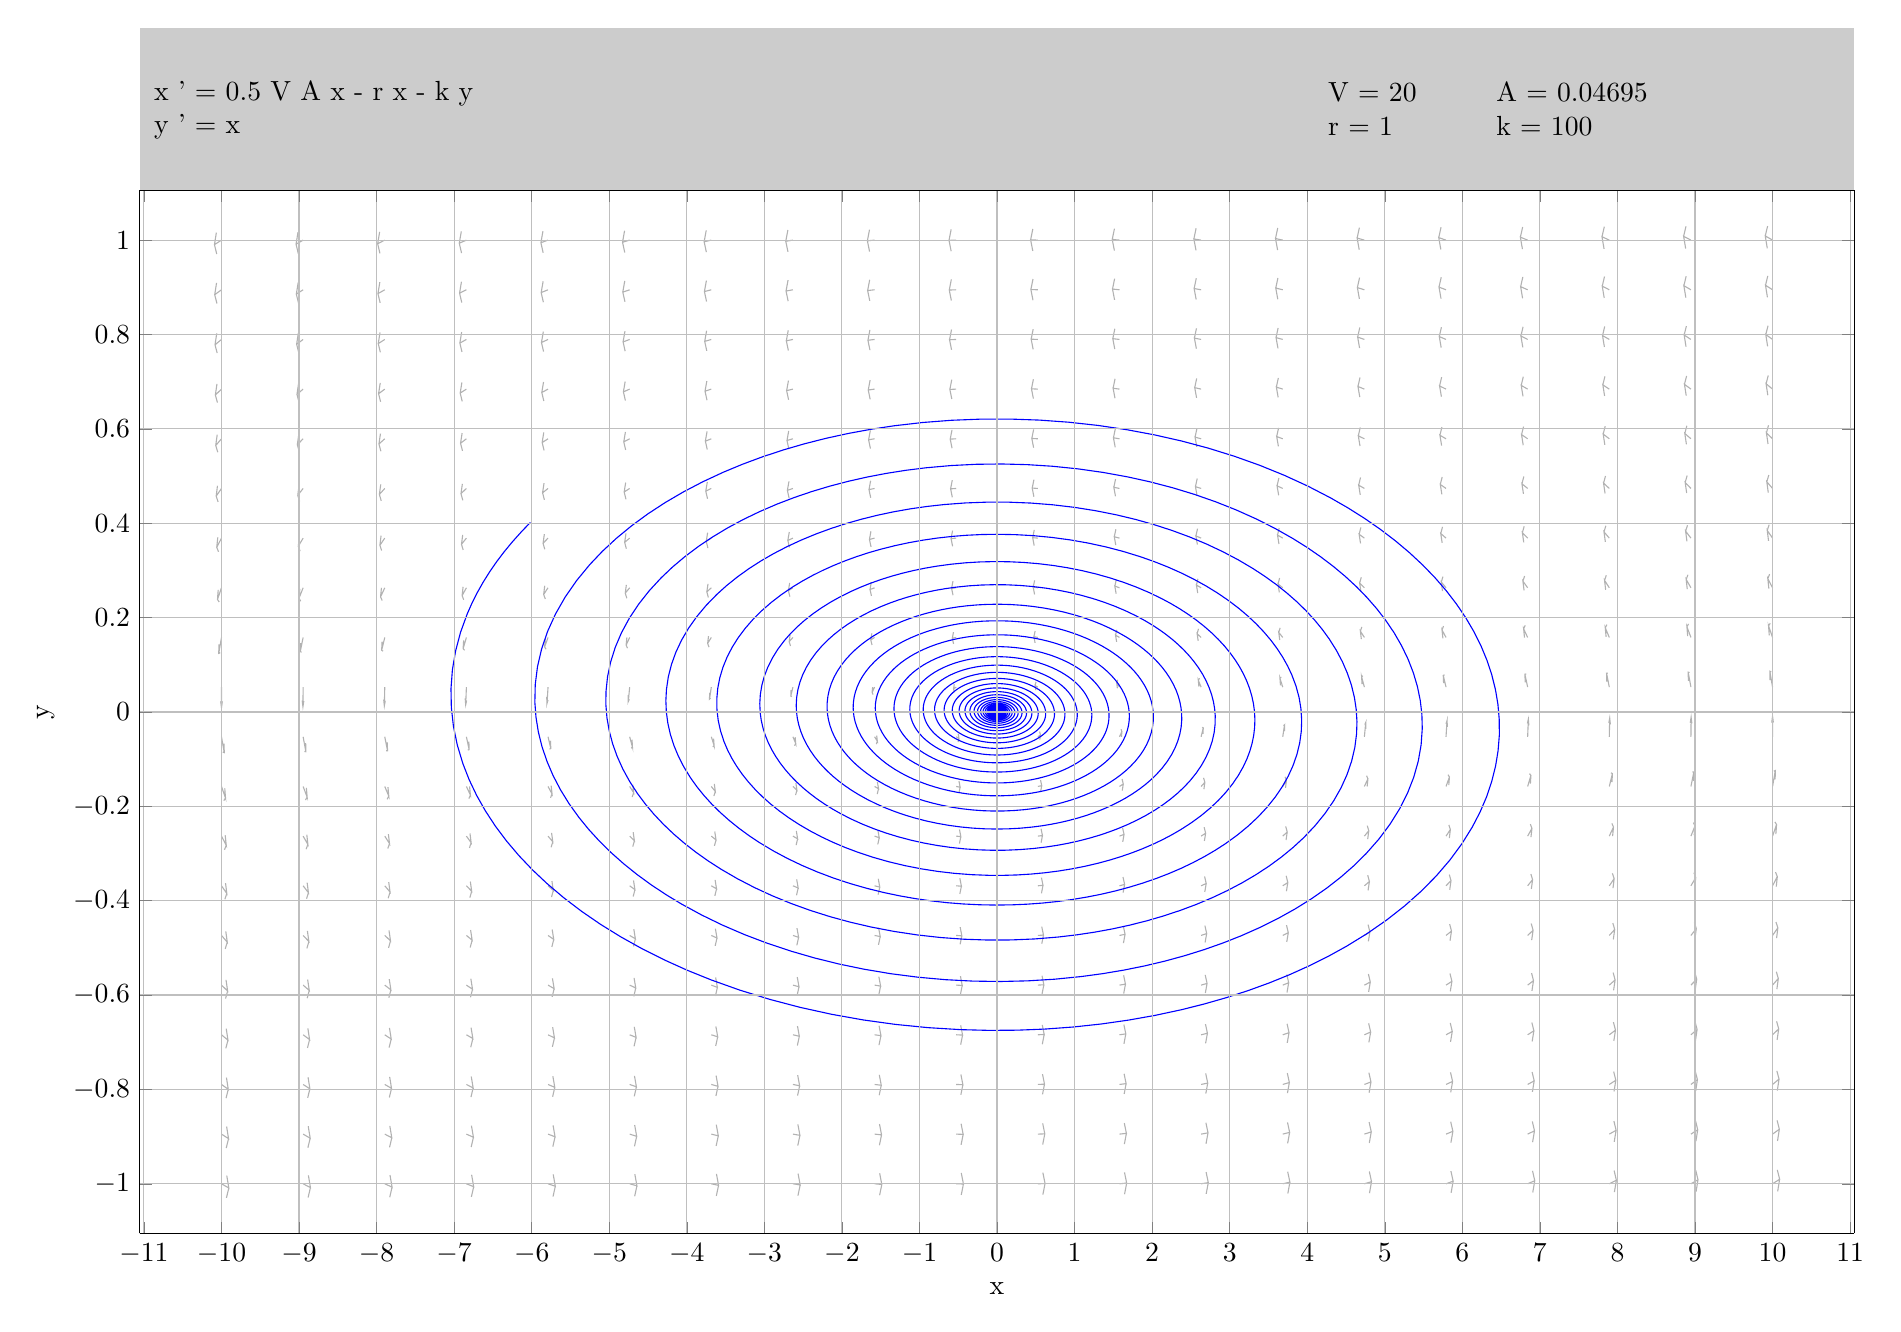
\begin{tikzpicture}

\begin{axis}[%
width=8.571659in,
height=0.813967in,
at={(0.866319in,6.91182in)},
scale only axis,
every outer x axis line/.append style={black},
every x tick label/.append style={font=\color{black}},
xmin=0,
xmax=1,
xtick={-1},
xticklabels={\empty},
every outer y axis line/.append style={black},
every y tick label/.append style={font=\color{black}},
ymin=0,
ymax=1,
ytick={-1},
yticklabels={\empty},
hide axis,
axis background/.style={fill=white!80!black},
axis x line*=bottom,
axis y line*=left
]
\node[right, align=left, inner sep=0mm, text=black]
at (axis cs:0.00806451612903225,0.495614035087719,0) {x ' = 0.5 V A x - r x - k y\\y ' = x};
\node[right, align=left, inner sep=0mm, text=black]
at (axis cs:0.790952380952381,0.5,0) {A = 0.04695\\k = 100};
\node[right, align=left, inner sep=0mm, text=black]
at (axis cs:0.692857142857143,0.5,0) {V = 20\\r = 1};
\node[right, align=left, inner sep=0mm, text=black]
at (axis cs:0.661428571428571,0.5,0) { \\ };
\end{axis}

\begin{axis}[%
width=8.571659in,
height=5.214906in,
at={(0.866319in,1.696914in)},
scale only axis,
unbounded coords=jump,
separate axis lines,
every outer x axis line/.append style={black},
every x tick label/.append style={font=\color{black}},
xmin=-11.0526315789474,
xmax=11.0526315789474,
xlabel={x},
xmajorgrids,
every outer y axis line/.append style={black},
every y tick label/.append style={font=\color{black}},
ymin=-1.10526315789474,
ymax=1.10526315789474,
ylabel={y},
ymajorgrids,
every outer z axis line/.append style={black},
every z tick label/.append style={font=\color{black}},
zmin=-1,
zmax=1,
view={0}{90}
]
\addplot [color=white!70!black,solid,forget plot]
  table[row sep=crcr]{%
-10	-1\\
-9.90568745073129	-1.00895613211801\\
-9.9317421824824	-0.98269115516543\\
-9.90568745073129	-1.00895613211801\\
-9.93622024854141	-1.02984742979978\\
nan	0\\
-10	-0.894736842105263\\
-9.90900440830407	-0.904337691964479\\
-9.93390287334804	-0.878708539082732\\
-9.90900440830407	-0.904337691964479\\
-9.93870329827765	-0.924206334930697\\
nan	0\\
-10	-0.789473684210526\\
-9.91259123428432	-0.799848320241985\\
-9.93622020499116	-0.774883738003628\\
-9.91259123428432	-0.799848320241985\\
-9.94140752300689	-0.818588120861466\\
nan	0\\
-10	-0.684210526315789\\
-9.916512653671	-0.695534521477473\\
-9.93872785877928	-0.671265486346717\\
-9.916512653671	-0.695534521477473\\
-9.94438985636012	-0.713009159511219\\
nan	0\\
-10	-0.578947368421053\\
-9.92086326766601	-0.591469055422963\\
-9.94147386561573	-0.567928366238891\\
-9.92086326766601	-0.591469055422963\\
-9.94773470911668	-0.607496732405888\\
nan	0\\
-10	-0.473684210526316\\
-9.92579086069872	-0.487772746607374\\
-9.94453146846884	-0.464993900957737\\
-9.92579086069872	-0.487772746607374\\
-9.95157573650937	-0.502098470608375\\
nan	0\\
-10	-0.368421052631579\\
-9.93154890962335	-0.384662047107772\\
-9.9480239881173	-0.362676976170752\\
-9.93154890962335	-0.384662047107772\\
-9.9561444853554	-0.396902521359076\\
nan	0\\
-10	-0.263157894736842\\
-9.93863635901856	-0.282564001289782\\
-9.95219392467476	-0.26140125907854\\
-9.93863635901856	-0.282564001289782\\
-9.96189697795123	-0.29208307956926\\
nan	0\\
-10	-0.157894736842105\\
-9.94826766072207	-0.182418856311678\\
-9.95765633263805	-0.162128535651323\\
-9.94826766072207	-0.182418856311678\\
-9.96991839237284	-0.18799470529029\\
nan	0\\
-10	-0.0526315789473685\\
-9.96447876631377	-0.0862431449743322\\
-9.9667322449129	-0.0672793667446849\\
-9.96447876631377	-0.0862431449743322\\
-9.98353802792638	-0.0850399835878012\\
nan	0\\
-10	0.0526315789473684\\
-9.99981942244857	0.00947467986285646\\
-9.98908437094287	0.0224668939760682\\
-9.99981942244857	0.00947467986285646\\
-10.0106628204851	0.0223766052003519\\
nan	0\\
-10	0.157894736842105\\
-10.0353382663378	0.124189405127673\\
-10.0163104535078	0.125466438057564\\
-10.0353382663378	0.124189405127673\\
-10.033163119365	0.143135571226442\\
nan	0\\
-10	0.263157894736842\\
-10.0516386416519	0.238580692763246\\
-10.030002748663	0.233044192942338\\
-10.0516386416519	0.238580692763246\\
-10.0422913496498	0.258863513768311\\
nan	0\\
-10	0.368421052631579\\
-10.0612995895681	0.348983761524292\\
-10.0380503899209	0.339490051464449\\
-10.0612995895681	0.348983761524292\\
-10.0477690354745	0.370139846248507\\
nan	0\\
-10	0.473684210526316\\
-10.0684009171473	0.457422832959875\\
-10.0438152976115	0.445201016942982\\
-10.0684009171473	0.457422832959875\\
-10.0519459863947	0.479401475516633\\
nan	0\\
-10	0.578947368421053\\
-10.0741670796235	0.564844411441787\\
-10.0483912164916	0.550533528629688\\
-10.0741670796235	0.564844411441787\\
-10.0554426949813	0.587617068441445\\
nan	0\\
-10	0.684210526315789\\
-10.0791000791629	0.671678044345698\\
-10.0522369349215	0.655662769146011\\
-10.0791000791629	0.671678044345698\\
-10.0585031759065	0.69521280872744\\
nan	0\\
-10	0.789473684210526\\
-10.0834546036201	0.778141267096646\\
-10.0555851182556	0.760677341325774\\
-10.0834546036201	0.778141267096646\\
-10.0612513268126	0.802404643135845\\
nan	0\\
-10	0.894736842105263\\
-10.0873790113822	0.884355426237614\\
-10.0585699540006	0.865625098152352\\
-10.0873790113822	0.884355426237614\\
-10.0637606619345	0.909314603843466\\
nan	0\\
-10	1\\
-10.0909682121894	0.990393556978788\\
-10.0612761377773	0.970533436837809\\
-10.0909682121894	0.990393556978788\\
-10.0660793592879	1.01601754293249\\
nan	0\\
-8.94736842105263	-1\\
-8.8531692784984	-1.00804641489822\\
-8.87941741754011	-0.982082704790198\\
-8.8531692784984	-1.00804641489822\\
-8.88344062498923	-1.02918227606731\\
nan	0\\
-8.94736842105263	-0.894736842105263\\
-8.8564885035489	-0.903367003778852\\
-8.88159493838162	-0.878057975900843\\
-8.8564885035489	-0.903367003778852\\
-8.88591001921842	-0.923497934652709\\
nan	0\\
-8.94736842105263	-0.789473684210526\\
-8.8600768443481	-0.798805660074825\\
-8.88393132339339	-0.774183173139403\\
-8.8600768443481	-0.798805660074825\\
-8.88859731132554	-0.817828961491667\\
nan	0\\
-8.94736842105263	-0.684210526315789\\
-8.86399831849292	-0.69440551290761\\
-8.88646060261288	-0.670504491290137\\
-8.86399831849292	-0.69440551290761\\
-8.89155809590879	-0.712189542569991\\
nan	0\\
-8.94736842105263	-0.578947368421053\\
-8.86834618478662	-0.590234504593347\\
-8.88923107162335	-0.567092804675155\\
-8.86834618478662	-0.590234504593347\\
-8.89487463970949	-0.606603922808163\\
nan	0\\
-8.94736842105263	-0.473684210526316\\
-8.87326556088808	-0.486406566679937\\
-8.89231582989904	-0.464064144792713\\
-8.87326556088808	-0.486406566679937\\
-8.89867700797585	-0.501115574874988\\
nan	0\\
-8.94736842105263	-0.368421052631579\\
-8.87900436417617	-0.383128861143508\\
-8.89583662911113	-0.361625504370814\\
-8.87900436417617	-0.383128861143508\\
-8.90319053336709	-0.395807532809045\\
nan	0\\
-8.94736842105263	-0.263157894736842\\
-8.88604983441457	-0.280820423822588\\
-8.90002977813455	-0.260192018437348\\
-8.88604983441457	-0.280820423822588\\
-8.90886104267742	-0.29085131175638\\
nan	0\\
-8.94736842105263	-0.157894736842105\\
-8.89560012334637	-0.180449705921042\\
-8.90549187038851	-0.160741140770795\\
-8.89560012334637	-0.180449705921042\\
-8.91676935492798	-0.186625289623927\\
nan	0\\
-8.94736842105263	-0.0526315789473685\\
-8.91187208875351	-0.0843605612059628\\
-8.9145887428786	-0.065967783453604\\
-8.91187208875351	-0.0843605612059628\\
-8.9304532340079	-0.0837159496031651\\
nan	0\\
-8.94736842105263	0.0526315789473684\\
-8.94976676153383	0.0110912955236224\\
-8.93866218853354	0.0229537954304461\\
-8.94976676153383	0.0110912955236224\\
-8.95943233024541	0.0241529656710463\\
nan	0\\
-8.94736842105263	0.157894736842105\\
-8.98506928006451	0.127348083685657\\
-8.96612235907184	0.127086864879621\\
-8.98506928006451	0.127348083685657\\
-8.98139568565006	0.145937294385562\\
nan	0\\
-8.94736842105263	0.263157894736842\\
-9.00025500329586	0.241219412784377\\
-8.97890440813478	0.234579311809308\\
-9.00025500329586	0.241219412784377\\
-8.98987364911101	0.261022602930925\\
nan	0\\
-8.94736842105263	0.368421052631579\\
-9.00946004739266	0.351111579303102\\
-8.98650519115853	0.340781514716638\\
-9.00946004739266	0.351111579303102\\
-8.99515992782277	0.371827327886652\\
nan	0\\
-8.94736842105263	0.473684210526316\\
-9.01634270541325	0.459204819132842\\
-8.9920305722567	0.446305065460728\\
-9.01634270541325	0.459204819132842\\
-8.99927026795344	0.48079220764104\\
nan	0\\
-8.94736842105263	0.578947368421053\\
-9.02198519420891	0.566385808693214\\
-8.99645977233007	0.551500083322496\\
-9.02198519420891	0.566385808693214\\
-9.00274055219399	0.588808469900635\\
nan	0\\
-8.94736842105263	0.684210526315789\\
-9.02683978653176	0.673043420492625\\
-9.00020660043223	0.656525710869793\\
-9.02683978653176	0.673043420492625\\
-9.00579015334381	0.696261393609356\\
nan	0\\
-8.94736842105263	0.789473684210526\\
-9.03114047683792	0.779372181897457\\
-9.00348348452407	0.761459618645054\\
-9.03114047683792	0.779372181897457\\
-9.0085342356806	0.803345646537701\\
nan	0\\
-8.94736842105263	0.894736842105263\\
-9.03502572311196	0.885480038466283\\
-9.00641433158441	0.866342754043146\\
-9.03502572311196	0.885480038466283\\
-9.0110427334039	0.910171405072808\\
nan	0\\
-8.94736842105263	1\\
-9.0385851716263	0.991431805130622\\
-9.00907809773685	0.971198075948019\\
-9.0385851716263	0.991431805130622\\
-9.01336219517154	1.01680645123485\\
nan	0\\
-7.89473684210526	-1\\
-7.80065696581268	-1.00712879352583\\
-7.827098730319	-0.981470186394933\\
-7.80065696581268	-1.00712879352583\\
-7.83066312708191	-1.02851012454122\\
nan	0\\
-7.89473684210526	-0.894736842105263\\
-7.80397942781037	-0.902386765342122\\
-7.82929417128962	-0.877402434797342\\
-7.80397942781037	-0.902386765342122\\
-7.83311913290805	-0.922781141944788\\
nan	0\\
-7.89473684210526	-0.789473684210526\\
-7.80757052369185	-0.7977511941496\\
-7.83165104173111	-0.773476361564524\\
-7.80757052369185	-0.7977511941496\\
-7.83578979670064	-0.817059520771231\\
nan	0\\
-7.89473684210526	-0.684210526315789\\
-7.81149366860865	-0.693261484780891\\
-7.83420388104136	-0.669735403867207\\
-7.81149366860865	-0.693261484780891\\
-7.83872936027391	-0.711356990615514\\
nan	0\\
-7.89473684210526	-0.578947368421053\\
-7.8158409272841	-0.588980123627948\\
-7.83700151292873	-0.566246318360589\\
-7.8158409272841	-0.588980123627948\\
-7.84201789053217	-0.60569427577117\\
nan	0\\
-7.89473684210526	-0.473684210526316\\
-7.82075493428576	-0.485012884872768\\
-7.840117338045	-0.463118805613956\\
-7.82075493428576	-0.485012884872768\\
-7.84578167521822	-0.500109759523709\\
nan	0\\
-7.89473684210526	-0.368421052631579\\
-7.82647812376933	-0.381554885489727\\
-7.84367228105557	-0.360550056048298\\
-7.82647812376933	-0.381554885489727\\
-7.85023919748464	-0.394679415216266\\
nan	0\\
-7.89473684210526	-0.263157894736842\\
-7.83348502513009	-0.279010498017308\\
-7.84789741940253	-0.258941762789375\\
-7.83348502513009	-0.279010498017308\\
-7.85582372104276	-0.289567671276961\\
nan	0\\
-7.89473684210526	-0.157894736842105\\
-7.84294905771168	-0.17836017228711\\
-7.8533690341685	-0.159273595555213\\
-7.84294905771168	-0.17836017228711\\
-7.86360175189101	-0.185167487752005\\
nan	0\\
-7.89473684210526	-0.0526315789473685\\
-7.85923423972591	-0.0822871009125809\\
-7.86247113994841	-0.0645147937281788\\
-7.85923423972591	-0.0822871009125809\\
-7.87729890093102	-0.0822660949178556\\
nan	0\\
-7.89473684210526	0.0526315789473684\\
-7.90013497081738	0.0129880388339239\\
-7.88860464717538	0.0235315686899288\\
-7.90013497081738	0.0129880388339239\\
-7.9084264172321	0.0262306330459858\\
nan	0\\
-7.89473684210526	0.157894736842105\\
-7.9346821082466	0.130711840522722\\
-7.91590280432435	0.128880392883203\\
-7.9346821082466	0.130711840522722\\
-7.92949425248404	0.14885302595387\\
nan	0\\
-7.89473684210526	0.263157894736842\\
-7.94877312153397	0.243878732188691\\
-7.92774244706832	0.23615341109596\\
-7.94877312153397	0.243878732188691\\
-7.9373820283424	0.263171550810314\\
nan	0\\
-7.89473684210526	0.368421052631579\\
-7.9575630513074	0.353231575450098\\
-7.93491781925139	0.342081866304008\\
-7.9575630513074	0.353231575450098\\
-7.94251255784213	0.373494970905076\\
nan	0\\
-7.89473684210526	0.473684210526316\\
-7.96424799862663	0.460975341978667\\
-7.94021743453331	0.44741021341262\\
-7.96424799862663	0.460975341978667\\
-7.94657186880713	0.482165791673303\\
nan	0\\
-7.89473684210526	0.578947368421053\\
-7.96977816138161	0.567916476497146\\
-7.94450804261773	0.552465414255231\\
-7.96977816138161	0.567916476497146\\
-7.95002348857968	0.589986073893405\\
nan	0\\
-7.89473684210526	0.684210526315789\\
-7.97456107359392	0.674399489403813\\
-7.94816104491933	0.657386742605242\\
-7.97456107359392	0.674399489403813\\
-7.95306656337532	0.69729885834957\\
nan	0\\
-7.89473684210526	0.789473684210526\\
-7.97881222985251	0.780595138590668\\
-7.95136997712337	0.762239855339815\\
-7.97881222985251	0.780595138590668\\
-7.9558092499333	0.804277549213437\\
nan	0\\
-7.89473684210526	0.894736842105263\\
-7.98266123030165	0.886597830284625\\
-7.95424916088757	0.86705843678172\\
-7.98266123030165	0.886597830284625\\
-7.95831866679789	0.911020630879912\\
nan	0\\
-7.89473684210526	1\\
-7.98619299722494	0.992464164539626\\
-7.95687219182394	0.971860876397819\\
-7.98619299722494	0.992464164539626\\
-7.96064010955413	1.01758895395766\\
nan	0\\
-6.84210526315789	-1\\
-6.74815070121638	-1.00620330633221\\
-6.77478624321578	-0.980853673947167\\
-6.74815070121638	-1.00620330633221\\
-6.77788789638188	-1.02783095491793\\
nan	0\\
-6.84210526315789	-0.894736842105263\\
-6.75147743165142	-0.901397018024991\\
-6.77700073712343	-0.876742007372454\\
-6.75147743165142	-0.901397018024991\\
-6.78033082508329	-0.922055923125692\\
nan	0\\
-6.84210526315789	-0.789473684210526\\
-6.75507261621714	-0.796684963048677\\
-6.77937959058983	-0.772763417662042\\
-6.75507261621714	-0.796684963048677\\
-6.7829852300089	-0.816279741132421\\
nan	0\\
-6.84210526315789	-0.684210526315789\\
-6.75899919526549	-0.692102465719655\\
-6.78195803078225	-0.668958366925395\\
-6.75899919526549	-0.692102465719655\\
-6.78590400048418	-0.710511400871596\\
nan	0\\
-6.84210526315789	-0.578947368421053\\
-6.76334823313135	-0.587705897464652\\
-6.78478570987841	-0.565389081244935\\
-6.76334823313135	-0.587705897464652\\
-6.78916497440021	-0.604767596258209\\
nan	0\\
-6.84210526315789	-0.473684210526316\\
-6.76826016331413	-0.483591547715677\\
-6.78793685896992	-0.462158071597927\\
-6.76826016331413	-0.483591547715677\\
-6.7928905275646	-0.49908062151981\\
nan	0\\
-6.84210526315789	-0.368421052631579\\
-6.77397224509471	-0.379939512312077\\
-6.79153253559354	-0.359450719892131\\
-6.77397224509471	-0.379939512312077\\
-6.79729176543379	-0.393517228923724\\
nan	0\\
-6.84210526315789	-0.263157894736842\\
-6.78094586001224	-0.277131904401646\\
-6.79580017853974	-0.257649850715791\\
-6.78094586001224	-0.277131904401646\\
-6.80278718337214	-0.288229552288618\\
nan	0\\
-6.84210526315789	-0.157894736842105\\
-6.79032197158219	-0.176139903469946\\
-6.80129566739794	-0.157720530587668\\
-6.79032197158219	-0.176139903469946\\
-6.81041825071186	-0.18361217637552\\
nan	0\\
-6.84210526315789	-0.0526315789473685\\
-6.80656207917971	-0.0799781531915263\\
-6.81038839081213	-0.0628883849237325\\
-6.80656207917971	-0.0799781531915263\\
-6.8240616779342	-0.0806599769128253\\
nan	0\\
-6.84210526315789	0.0526315789473684\\
-6.85101778202662	0.0152986499016179\\
-6.83901079410457	0.0242703988981606\\
-6.85101778202662	0.0152986499016179\\
-6.85767725862744	0.0287266583325255\\
nan	0\\
-6.84210526315789	0.157894736842105\\
-6.88413350790854	0.134246061024227\\
-6.86561286552887	0.13083360258193\\
-6.88413350790854	0.134246061024227\\
-6.87743720343781	0.151847724957251\\
nan	0\\
-6.84210526315789	0.263157894736842\\
-6.89719057662392	0.24654418413194\\
-6.87651155493289	0.237756968946903\\
-6.89719057662392	0.24654418413194\\
-6.88481841023534	0.265299625679918\\
nan	0\\
-6.84210526315789	0.368421052631579\\
-6.90560944125468	0.355338508632304\\
-6.88328755182583	0.343387227307889\\
-6.90560944125468	0.355338508632304\\
-6.88982882382547	0.375139316356283\\
nan	0\\
-6.84210526315789	0.473684210526316\\
-6.91211763820017	0.462732074027257\\
-6.88837589156272	0.448514621216406\\
-6.91211763820017	0.462732074027257\\
-6.89385195981225	0.483520808737543\\
nan	0\\
-6.84210526315789	0.578947368421053\\
-6.91754659512143	0.569435205249813\\
-6.89253615473956	0.553428521210301\\
-6.91754659512143	0.569435205249813\\
-6.89729223632518	0.591149187192068\\
nan	0\\
-6.84210526315789	0.684210526315789\\
-6.92226437747386	0.67574554777247\\
-6.89610039854324	0.658245262756475\\
-6.92226437747386	0.67574554777247\\
-6.9003328878149	0.698324819914457\\
nan	0\\
-6.84210526315789	0.789473684210526\\
-6.92647017957409	0.781809693368858\\
-6.89924470693882	0.763017661517309\\
-6.92647017957409	0.781809693368858\\
-6.90307670235965	0.805200119725409\\
nan	0\\
-6.84210526315789	0.894736842105263\\
-6.93028576863237	0.88770850383436\\
-6.9020745324223	0.867771878947013\\
-6.93028576863237	0.88770850383436\\
-6.90558870155775	0.91186213168425\\
nan	0\\
-6.84210526315789	1\\
-6.93379186865998	0.993490425516022\\
-6.90465849338836	0.972521646485693\\
-6.93379186865998	0.993490425516022\\
-6.90791328063035	1.01836494923674\\
nan	0\\
-5.78947368421053	-1\\
-5.69565067545287	-1.00527000005788\\
-5.7224800780657	-0.980233247851099\\
-5.69565067545287	-1.00527000005788\\
-5.72511507809464	-1.02714475222993\\
nan	0\\
-5.78947368421053	-0.894736842105263\\
-5.69898276925013	-0.900397815370413\\
-5.72471480042196	-0.87607679465077\\
-5.69898276925013	-0.900397815370413\\
-5.72754528705454	-0.921322252130966\\
nan	0\\
-5.78947368421053	-0.789473684210526\\
-5.7025834720997	-0.795607025671356\\
-5.72711720036774	-0.7720444702054\\
-5.7025834720997	-0.795607025671356\\
-5.73018387109815	-0.815489576260814\\
nan	0\\
-5.78947368421053	-0.684210526315789\\
-5.70651540137656	-0.690928513227706\\
-5.72972338949877	-0.668173546445639\\
-5.70651540137656	-0.690928513227706\\
-5.73308238295473	-0.709652687862624\\
nan	0\\
-5.78947368421053	-0.578947368421053\\
-5.71086886399356	-0.586411859206577\\
-5.73258418736227	-0.564521306916678\\
-5.71086886399356	-0.586411859206577\\
-5.73631643275503	-0.603823717025161\\
nan	0\\
-5.78947368421053	-0.473684210526316\\
-5.71578248444755	-0.482142487442414\\
-5.73577527514742	-0.46118220442684\\
-5.71578248444755	-0.482142487442414\\
-5.74000441360547	-0.498027804308329\\
nan	0\\
-5.78947368421053	-0.368421052631579\\
-5.72148892923341	-0.378282295779554\\
-5.73941904493955	-0.358327734090883\\
-5.72148892923341	-0.378282295779554\\
-5.74434966651354	-0.39232011157944\\
nan	0\\
-5.78947368421053	-0.263157894736842\\
-5.72843674667853	-0.275182615798746\\
-5.74374164767266	-0.256315965097176\\
-5.72843674667853	-0.275182615798746\\
-5.74975400820361	-0.286834433863173\\
nan	0\\
-5.78947368421053	-0.157894736842105\\
-5.73772840522271	-0.173778373706835\\
-5.74928107970287	-0.156076962900461\\
-5.73772840522271	-0.173778373706835\\
-5.75722289813523	-0.181949602394371\\
nan	0\\
-5.78947368421053	-0.0526315789473685\\
-5.75385499481212	-0.0773738089610982\\
-5.75835504412821	-0.0610464676073789\\
-5.75385499481212	-0.0773738089610982\\
-5.77072615913508	-0.0788558123065797\\
nan	0\\
-5.78947368421053	0.0526315789473684\\
-5.80249671217905	0.0182328977962719\\
-5.78999013350072	0.0252967451494703\\
-5.80249671217905	0.0182328977962719\\
-5.80718947407627	0.0318082591337313\\
nan	0\\
-5.78947368421053	0.157894736842105\\
-5.83338726048343	0.137904696121135\\
-5.81521567742131	0.132923314269202\\
-5.83338726048343	0.137904696121135\\
-5.8252106977818	0.154880102405651\\
nan	0\\
-5.78947368421053	0.263157894736842\\
-5.84550700453633	0.249201741636867\\
-5.8252079701636	0.239380257485408\\
-5.84550700453633	0.249201741636867\\
-5.83218604671358	0.267396917648311\\
nan	0\\
-5.78947368421053	0.368421052631579\\
-5.85360053205307	0.357427507505099\\
-5.83161409141869	0.344693859082407\\
-5.85360053205307	0.357427507505099\\
-5.83711086398193	0.376757283003679\\
nan	0\\
-5.78947368421053	0.473684210526316\\
-5.85995261209359	0.464472865996096\\
-5.83650609759611	0.449616537384397\\
-5.85995261209359	0.464472865996096\\
-5.84111176986122	0.484856001325927\\
nan	0\\
-5.78947368421053	0.578947368421053\\
-5.86529116576573	0.570940875833778\\
-5.84054429815235	0.55438845322116\\
-5.86529116576573	0.570940875833778\\
-5.84454754444599	0.59229719399876\\
nan	0\\
-5.78947368421053	0.684210526315789\\
-5.86995016065465	0.677080942248803\\
-5.84402482170466	0.659100698357869\\
-5.86995016065465	0.677080942248803\\
-5.84758961373816	0.699338936579929\\
nan	0\\
-5.78947368421053	0.789473684210526\\
-5.87411465571487	0.783015432098891\\
-5.84710780123566	0.763792664856297\\
-5.87411465571487	0.783015432098891\\
-5.85033692729147	0.806113150608467\\
nan	0\\
-5.78947368421053	0.894736842105263\\
-5.87789958083712	0.888811779970072\\
-5.84989054631534	0.868482824453981\\
-5.87789958083712	0.888811779970072\\
-5.85285307738294	0.912695772767278\\
nan	0\\
-5.78947368421053	1\\
-5.8813819697644	0.994510390758845\\
-5.85243708178795	0.973180202142723\\
-5.8813819697644	0.994510390758845\\
-5.85518188640853	1.01913434491966\\
nan	0\\
-4.73684210526316	-1\\
-4.64315708121373	-1.00432893020619\\
-4.67018035587701	-0.979608995131972\\
-4.64315708121373	-1.00432893020619\\
-4.6723448209801	-1.02645150715669\\
nan	0\\
-4.73684210526316	-0.894736842105263\\
-4.64649569800634	-0.89938922369017\\
-4.67243652478716	-0.875406907400493\\
-4.64649569800634	-0.89938922369017\\
-4.67476271557961	-0.920580111028904\\
nan	0\\
-4.73684210526316	-0.789473684210526\\
-4.65010344715354	-0.794517460304047\\
-4.67486410056305	-0.771319662948586\\
-4.65010344715354	-0.794517460304047\\
-4.67738598860981	-0.814688992003395\\
nan	0\\
-4.73684210526316	-0.684210526315789\\
-4.65404280045042	-0.689739715764199\\
-4.67750029453214	-0.667381132726492\\
-4.65404280045042	-0.689739715764199\\
-4.68026488925635	-0.70878078513286\\
nan	0\\
-4.73684210526316	-0.578947368421053\\
-4.65840360336421	-0.585098094558745\\
-4.68039747239947	-0.563643251242699\\
-4.65840360336421	-0.585098094558745\\
-4.68347283546832	-0.602862502192175\\
nan	0\\
-4.73684210526316	-0.473684210526316\\
-4.66332318499919	-0.48066573279629\\
-4.68363348051089	-0.460191546049307\\
-4.66332318499919	-0.48066573279629\\
-4.68712424164588	-0.496951006181289\\
nan	0\\
-4.73684210526316	-0.368421052631579\\
-4.66903051762849	-0.376582983352775\\
-4.68733351123859	-0.357181507227748\\
-4.66903051762849	-0.376582983352775\\
-4.69141447659919	-0.391087301045084\\
nan	0\\
-4.73684210526316	-0.263157894736842\\
-4.67596258741696	-0.273161010431477\\
-4.69172566384716	-0.254940196261537\\
-4.67596258741696	-0.273161010431477\\
-4.69672722169448	-0.285379955184636\\
nan	0\\
-4.73684210526316	-0.157894736842105\\
-4.68518032201721	-0.17126534027892\\
-4.69733620613179	-0.154338713436389\\
-4.68518032201721	-0.17126534027892\\
-4.7040215078502	-0.180169605059361\\
nan	0\\
-4.73684210526316	-0.0526315789473685\\
-4.70111874551426	-0.0743927375476681\\
-4.70639546378885	-0.0589335500303525\\
-4.70111874551426	-0.0743927375476681\\
-4.717276043089	-0.0767952299048039\\
nan	0\\
-4.73684210526316	0.0526315789473684\\
-4.75457224314528	0.0220945507320524\\
-4.74161894472682	0.0268231247261157\\
-4.75457224314528	0.0220945507320524\\
-4.75688745883448	0.0356881936671787\\
nan	0\\
-4.73684210526316	0.157894736842105\\
-4.7824180684447	0.141634061389333\\
-4.76468011062705	0.135118273229778\\
-4.7824180684447	0.141634061389333\\
-4.77281044835343	0.157906254820551\\
nan	0\\
-4.73684210526316	0.263157894736842\\
-4.79372394599214	0.251838250585625\\
-4.77382948273564	0.241013683648744\\
-4.79372394599214	0.251838250585625\\
-4.77948930481125	0.269454604013236\\
nan	0\\
-4.73684210526316	0.368421052631579\\
-4.80153805099484	0.359494122035645\\
-4.77989753462635	0.345998214781505\\
-4.80153805099484	0.359494122035645\\
-4.78436099992432	0.378346187647344\\
nan	0\\
-4.73684210526316	0.473684210526316\\
-4.80775403363709	0.466195755130156\\
-4.78460834127587	0.45071430965552\\
-4.80775403363709	0.466195755130156\\
-4.78835256897395	0.486170273842488\\
nan	0\\
-4.73684210526316	0.578947368421053\\
-4.81301259171371	0.572432461121444\\
-4.78853271895365	0.555344311698687\\
-4.81301259171371	0.572432461121444\\
-4.79179017260345	0.593429554923965\\
nan	0\\
-4.73684210526316	0.684210526315789\\
-4.81761890725869	0.678405069615998\\
-4.79193450248508	0.659952506127053\\
-4.81761890725869	0.678405069615998\\
-4.79483723083498	0.700340907124817\\
nan	0\\
-4.73684210526316	0.789473684210526\\
-4.82174599893253	0.784211970234507\\
-4.79495940233771	0.76456451100997\\
-4.82174599893253	0.784211970234507\\
-4.79759025932572	0.807016457844656\\
nan	0\\
-4.73684210526316	0.894736842105263\\
-4.82550291569255	0.889907398140109\\
-4.79769731157244	0.869191028722308\\
-4.82550291569255	0.889907398140109\\
-4.80011203355502	0.913521433937003\\
nan	0\\
-4.73684210526316	1\\
-4.82896348794376	0.99552387525408\\
-4.8002080419531	0.973836367007704\\
-4.82896348794376	0.99552387525408\\
-4.80244610432606	1.01989705834801\\
nan	0\\
-3.68421052631579	-1\\
-3.59067011286216	-1.00338016139389\\
-3.61788719654978	-0.978981009612316\\
-3.59067011286216	-1.00338016139389\\
-3.61957727724672	-1.02575121633913\\
nan	0\\
-3.68421052631579	-0.894736842105263\\
-3.5940164781049	-0.898371322657876\\
-3.62016607243001	-0.874732466439369\\
-3.5940164781049	-0.898371322657876\\
-3.62198331270632	-0.919829490544814\\
nan	0\\
-3.68421052631579	-0.789473684210526\\
-3.59763290210993	-0.793416365688998\\
-3.62262051900207	-0.770589155193992\\
-3.59763290210993	-0.793416365688998\\
-3.62459185974131	-0.81387796729692\\
nan	0\\
-3.68421052631579	-0.684210526315789\\
-3.60158191533818	-0.688536194829764\\
-3.62528908150297	-0.666581341531168\\
-3.60158191533818	-0.688536194829764\\
-3.62745191575995	-0.707895647019975\\
nan	0\\
-3.68421052631579	-0.578947368421053\\
-3.60595325426413	-0.583764746343301\\
-3.62822609139906	-0.562755214953712\\
-3.60595325426413	-0.583764746343301\\
-3.63063478036019	-0.601883850979542\\
nan	0\\
-3.68421052631579	-0.473684210526316\\
-3.61088359870783	-0.479161420248028\\
-3.63151237455979	-0.459186525429525\\
-3.61088359870783	-0.479161420248028\\
-3.63425097942065	-0.495849989233504\\
nan	0\\
-3.68421052631579	-0.368421052631579\\
-3.61659948413656	-0.374841549491104\\
-3.63527767257545	-0.356012639888439\\
-3.61659948413656	-0.374841549491104\\
-3.63848792100521	-0.389818160978054\\
nan	0\\
-3.68421052631579	-0.263157894736842\\
-3.6235287800207	-0.271066003947109\\
-3.63975627660666	-0.253523134610255\\
-3.6235287800207	-0.271066003947109\\
-3.64371033121179	-0.283864007757802\\
nan	0\\
-3.68421052631579	-0.157894736842105\\
-3.63269248604206	-0.168591528391962\\
-3.64547370023672	-0.152502980858573\\
-3.63269248604206	-0.168591528391962\\
-3.65082209601164	-0.178262000995437\\
nan	0\\
-3.68421052631579	-0.0526315789473685\\
-3.64837362917068	-0.0709243765567166\\
-3.65455149891187	-0.0564773129876337\\
-3.64837362917068	-0.0709243765567166\\
-3.66369789771655	-0.0743957615601905\\
nan	0\\
-3.68421052631579	0.0526315789473684\\
-3.70702426958202	0.0272285402352631\\
-3.69382938692413	0.0291460160323358\\
-3.70702426958202	0.0272285402352631\\
-3.70653090628018	0.0405528876654536\\
nan	0\\
-3.68421052631579	0.157894736842105\\
-3.7312137510015	0.145377947889601\\
-3.71398358635766	0.137382178403924\\
-3.7312137510015	0.145377947889601\\
-3.72024198083392	0.160883790746781\\
nan	0\\
-3.68421052631579	0.263157894736842\\
-3.74184460765643	0.254441777307689\\
-3.72237535389695	0.242648092201273\\
-3.74184460765643	0.254441777307689\\
-3.72673341261153	0.271465132871596\\
nan	0\\
-3.68421052631579	0.368421052631579\\
-3.74942407084401	0.361534359086173\\
-3.72813833409919	0.34729698101774\\
-3.74942407084401	0.361534359086173\\
-3.73158168087189	0.37990375328185\\
nan	0\\
-3.68421052631579	0.473684210526316\\
-3.75552312032281	0.467898969984062\\
-3.73268303198514	0.451806393644983\\
-3.75552312032281	0.467898969984062\\
-3.73557565225627	0.487462690648494\\
nan	0\\
-3.68421052631579	0.578947368421053\\
-3.76071163130459	0.573909026440447\\
-3.7365017143128	0.556295252787428\\
-3.76071163130459	0.573909026440447\\
-3.7390208853031	0.59454580528183\\
nan	0\\
-3.68421052631579	0.684210526315789\\
-3.76527111943753	0.679717376597869\\
-3.73982965407152	0.660800173232811\\
-3.76527111943753	0.679717376597869\\
-3.74207622893048	0.701330469793679\\
nan	0\\
-3.68421052631579	0.789473684210526\\
-3.76936455903393	0.785398952577553\\
-3.74279966631024	0.765332863887911\\
-3.76936455903393	0.785398952577553\\
-3.74483703212673	0.807909880246979\\
nan	0\\
-3.68421052631579	0.894736842105263\\
-3.77309602704402	0.890995116197883\\
-3.7454949453487	0.86989625878804\\
-3.77309602704402	0.890995116197883\\
-3.74736580830239	0.914339009152154\\
nan	0\\
-3.68421052631579	1\\
-3.77653661360967	0.996530706137819\\
-3.74797146395596	0.974489972473002\\
-3.77653661360967	0.996530706137819\\
-3.74970611088705	1.02065301611994\\
nan	0\\
-2.63157894736842	-1\\
-2.53818996613236	-1.00242376769666\\
-2.56560071857902	-0.978349392078646\\
-2.53818996613236	-1.00242376769666\\
-2.56681260242735	-1.02504388269667\\
nan	0\\
-2.63157894736842	-0.894736842105263\\
-2.5415453720344	-0.897344205894783\\
-2.56790360368723	-0.874053602924422\\
-2.5415453720344	-0.897344205894783\\
-2.56920728558199	-0.919070390591432\\
nan	0\\
-2.63157894736842	-0.789473684210526\\
-2.54517220180769	-0.792303862083824\\
-2.57038668100759	-0.769853122331653\\
-2.54517220180769	-0.792303862083824\\
-2.57180176994424	-0.813056495112017\\
nan	0\\
-2.63157894736842	-0.684210526315789\\
-2.54913327678768	-0.687318107046675\\
-2.57309008277918	-0.665774415182223\\
-2.54913327678768	-0.687318107046675\\
-2.57464387314462	-0.706997250472595\\
nan	0\\
-2.63157894736842	-0.578947368421053\\
-2.55351863647024	-0.582412019045681\\
-2.57607056708353	-0.561857546133746\\
-2.55351863647024	-0.582412019045681\\
-2.57780289239585	-0.600887701582839\\
nan	0\\
-2.63157894736842	-0.473684210526316\\
-2.55846509998769	-0.477629805484937\\
-2.57941285546225	-0.458167665152168\\
-2.55846509998769	-0.477629805484937\\
-2.58138565294157	-0.494724588842533\\
nan	0\\
-2.63157894736842	-0.368421052631579\\
-2.56419842242438	-0.373058231320822\\
-2.58325328523528	-0.354821946478038\\
-2.56419842242438	-0.373058231320822\\
-2.5855718745799	-0.38851220895006\\
nan	0\\
-2.63157894736842	-0.263157894736842\\
-2.57114119775284	-0.268897199576648\\
-2.58783769642757	-0.252065970720812\\
-2.57114119775284	-0.268897199576648\\
-2.59070734884747	-0.282284845528601\\
nan	0\\
-2.63157894736842	-0.157894736842105\\
-2.5802827574838	-0.165749600923665\\
-2.59370789842879	-0.150569094228041\\
-2.5802827574838	-0.165749600923665\\
-2.59763533046957	-0.176217189170353\\
nan	0\\
-2.63157894736842	-0.0526315789473685\\
-2.59567130318549	-0.0668215193476579\\
-2.6028961113403	-0.053587626181838\\
-2.59567130318549	-0.0668215193476579\\
-2.60999108154044	-0.0715414482733041\\
nan	0\\
-2.63157894736842	0.0526315789473684\\
-2.65927544800445	0.0337840113148193\\
-2.64625460590551	0.0325141564455763\\
-2.65927544800445	0.0337840113148193\\
-2.65567838972178	0.0463624067635917\\
nan	0\\
-2.63157894736842	0.157894736842105\\
-2.67977529143566	0.149082899550353\\
-2.66311342889255	0.139677364721068\\
-2.67977529143566	0.149082899550353\\
-2.66751934753843	0.163775536754689\\
nan	0\\
-2.63157894736842	0.263157894736842\\
-2.68987356535837	0.257001855031477\\
-2.67084617003505	0.244275012445598\\
-2.68987356535837	0.257001855031477\\
-2.67392418988773	0.273422321440575\\
nan	0\\
-2.63157894736842	0.368421052631579\\
-2.69726094137665	0.36354470280358\\
-2.67633725571718	0.348587109249922\\
-2.69726094137665	0.36354470280358\\
-2.67877543063118	0.381428106254037\\
nan	0\\
-2.63157894736842	0.473684210526316\\
-2.70326117305131	0.469580931916001\\
-2.68073068569386	0.452891359078374\\
-2.70326117305131	0.469580931916001\\
-2.68278232499902	0.488732471919818\\
nan	0\\
-2.63157894736842	0.578947368421053\\
-2.70838907497547	0.575369729090512\\
-2.68445162686072	0.557240488987911\\
-2.70838907497547	0.575369729090512\\
-2.68624044652599	0.595645552791436\\
nan	0\\
-2.63157894736842	0.684210526315789\\
-2.71290731390009	0.681017359330506\\
-2.68771051219427	0.661643217793175\\
-2.71290731390009	0.681017359330506\\
-2.68930709568691	0.702307401059008\\
nan	0\\
-2.63157894736842	0.789473684210526\\
-2.71697069324849	0.786576052900865\\
-2.69062876165706	0.766097405823745\\
-2.71697069324849	0.786576052900865\\
-2.69207757731189	0.808793278763781\\
nan	0\\
-2.63157894736842	0.894736842105263\\
-2.72067917286779	0.892074710149322\\
-2.69328357222899	0.870598293361263\\
-2.72067917286779	0.892074710149322\\
-2.69461463820696	0.915148406110945\\
nan	0\\
-2.63157894736842	1\\
-2.72410153963402	0.997530722527239\\
-2.69572744258615	0.975140857702667\\
-2.72410153963402	0.997530722527239\\
-2.69696208132253	1.02140215383547\\
nan	0\\
-1.57894736842105	-1\\
-1.48571683780412	-1.00145983298764\\
-1.51332103874229	-0.977714250437112\\
-1.48571683780412	-1.00145983298764\\
-1.51405095523611	-1.02432951574558\\
nan	0\\
-1.57894736842105	-0.894736842105263\\
-1.48908264405994	-0.896307981544474\\
-1.51564927650847	-0.873370458622433\\
-1.48908264405994	-0.896307981544474\\
-1.51643484622808	-0.918302820802988\\
nan	0\\
-1.57894736842105	-0.789473684210526\\
-1.49272171429173	-0.791180092303249\\
-1.51816280850735	-0.769111756343102\\
-1.49272171429173	-0.791180092303249\\
-1.51901601255371	-0.812224583407763\\
nan	0\\
-1.57894736842105	-0.684210526315789\\
-1.4966974217961	-0.6860856462124\\
-1.52090362580943	-0.664960623587179\\
-1.4966974217961	-0.6860856462124\\
-1.52184118575774	-0.706085596899655\\
nan	0\\
-1.57894736842105	-0.578947368421053\\
-1.50110058324326	-0.58104018333557\\
-1.52393141506797	-0.560950642566766\\
-1.50110058324326	-0.58104018333557\\
-1.52497782252522	-0.599874035155664\\
nan	0\\
-1.57894736842105	-0.473684210526316\\
-1.50606909671272	-0.47607127499327\\
-1.52733581210848	-0.4571355877261\\
-1.50606909671272	-0.47607127499327\\
-1.52852934434196	-0.493574723580267\\
nan	0\\
-1.57894736842105	-0.368421052631579\\
-1.51183002797592	-0.37123356558822\\
-1.5312621018703	-0.353610476589945\\
-1.51183002797592	-0.37123356558822\\
-1.53266835834862	-0.387169146812511\\
nan	0\\
-1.57894736842105	-0.263157894736842\\
-1.5188061418987	-0.266655053756585\\
-1.53597422010047	-0.250570599420075\\
-1.5188061418987	-0.266655053756585\\
-1.53772279961034	-0.280641212681249\\
nan	0\\
-1.57894736842105	-0.157894736842105\\
-1.52797219617795	-0.162735454020122\\
-1.54205456855637	-0.148539445805941\\
-1.52797219617795	-0.162735454020122\\
-1.54447492714538	-0.174027031927494\\
nan	0\\
-1.57894736842105	-0.0526315789473685\\
-1.54312708855442	-0.061902237585155\\
-1.55155550785496	-0.0501659700271605\\
-1.54312708855442	-0.061902237585155\\
-1.55619083717386	-0.0680761099604775\\
nan	0\\
-1.57894736842105	0.0526315789473684\\
-1.61054797633237	0.041357056293632\\
-1.59824916329554	0.0368392611119245\\
-1.61054797633237	0.041357056293632\\
-1.60388642462241	0.0526395650675814\\
nan	0\\
-1.57894736842105	0.157894736842105\\
-1.62811495344507	0.152702531865706\\
-1.61206662669376	0.141968297102623\\
-1.62811495344507	0.152702531865706\\
-1.61466272918196	0.166552089614629\\
nan	0\\
-1.57894736842105	0.263157894736842\\
-1.63781644033298	0.259509626029161\\
-1.61924365158248	0.245886838663484\\
-1.63781644033298	0.259509626029161\\
-1.62106778593632	0.275321374619447\\
nan	0\\
-1.57894736842105	0.368421052631579\\
-1.64505122221396	0.365522121045903\\
-1.62449533317967	0.349865837073378\\
-1.64505122221396	0.365522121045903\\
-1.62594479897251	0.382917763969833\\
nan	0\\
-1.57894736842105	0.473684210526316\\
-1.65096955624345	0.471240253627746\\
-1.62875191067209	0.453967893741717\\
-1.65096955624345	0.471240253627746\\
-1.62997388912137	0.489978987652917\\
nan	0\\
-1.57894736842105	0.578947368421053\\
-1.65604573778715	0.576813817010432\\
-1.63238283912467	0.558179290092094\\
-1.65604573778715	0.576813817010432\\
-1.63344961482998	0.596728474775142\\
nan	0\\
-1.57894736842105	0.684210526315789\\
-1.66052801860382	0.682304562531863\\
-1.63557733260301	0.66248118912135\\
-1.66052801860382	0.682304562531863\\
-1.63653031449497	0.703271514212732\\
nan	0\\
-1.57894736842105	0.789473684210526\\
-1.66456476457973	0.787742973446142\\
-1.63844686804103	0.766857837635788\\
-1.66456476457973	0.787742973446142\\
-1.63931222342322	0.809666535715127\\
nan	0\\
-1.57894736842105	0.894736842105263\\
-1.66825261437341	0.893145973842337\\
-1.64106332352197	0.871296922833126\\
-1.66825261437341	0.893145973842337\\
-1.64185875765343	0.915949545809303\\
nan	0\\
-1.57894736842105	1\\
-1.67165846082534	0.99852377532217\\
-1.64347607693459	0.975788869624448\\
-1.67165846082534	0.99852377532217\\
-1.64421418927351	1.02214441582659\\
nan	0\\
-0.526315789473685	-1\\
-0.433250925352403	-1.00048845126697\\
-0.461048271772046	-0.977075699856558\\
-0.433250925352403	-1.00048845126697\\
-0.46129249740553	-1.0236081319172\\
nan	0\\
-0.526315789473685	-0.894736842105263\\
-0.436628559649206	-0.895262772832168\\
-0.463403245914824	-0.872683186157977\\
-0.436628559649206	-0.895262772832168\\
-0.463666211278276	-0.917526801070216\\
nan	0\\
-0.526315789473685	-0.789473684210526\\
-0.440281809817367	-0.790045222733658\\
-0.465949119083479	-0.768365266262639\\
-0.440281809817367	-0.790045222733658\\
-0.466234888345045	-0.811382256090798\\
nan	0\\
-0.526315789473685	-0.684210526315789\\
-0.44427489175346	-0.684839045303461\\
-0.468730031322609	-0.664140265177103\\
-0.44427489175346	-0.684839045303461\\
-0.469044290816445	-0.705160714037216\\
nan	0\\
-0.526315789473685	-0.578947368421053\\
-0.448699937528756	-0.579649580497764\\
-0.471809140093057	-0.560034953888518\\
-0.448699937528756	-0.579649580497764\\
-0.472160246131413	-0.598842879860983\\
nan	0\\
-0.526315789473685	-0.473684210526316\\
-0.453697021421734	-0.474486357516026\\
-0.475282115089892	-0.456091021406125\\
-0.453697021421734	-0.474486357516026\\
-0.475683188584747	-0.492400405432101\\
nan	0\\
-0.526315789473685	-0.368421052631579\\
-0.459497074021505	-0.36936842597293\\
-0.479305845321821	-0.35237953510748\\
-0.459497074021505	-0.36936842597293\\
-0.479779531992497	-0.38578889283357\\
nan	0\\
-0.526315789473685	-0.263157894736842\\
-0.466530260044861	-0.264341052026575\\
-0.484170129551075	-0.249039722482449\\
-0.466530260044861	-0.264341052026575\\
-0.484761708195941	-0.278932487196861\\
nan	0\\
-0.526315789473685	-0.157894736842105\\
-0.475784818129523	-0.15954983490287\\
-0.49053033501758	-0.1464205626486\\
-0.475784818129523	-0.15954983490287\\
-0.491357884047962	-0.171686048320681\\
nan	0\\
-0.526315789473685	-0.0526315789473685\\
-0.490971579086962	-0.0559879447786892\\
-0.500735750745149	-0.0461449824326122\\
-0.490971579086962	-0.0559879447786892\\
-0.502413933660809	-0.0638170876259738\\
nan	0\\
-0.526315789473685	0.0526315789473684\\
-0.560406688882678	0.0490315050882424\\
-0.549279400595198	0.041588802393732\\
-0.560406688882678	0.0490315050882424\\
-0.551079437524761	0.0586342520982284\\
nan	0\\
-0.526315789473685	0.157894736842105\\
-0.576253185403744	0.156200191772455\\
-0.560848330357314	0.144224206310835\\
-0.576253185403744	0.156200191772455\\
-0.561695602892139	0.169192904275865\\
nan	0\\
-0.526315789473685	0.263157894736842\\
-0.585679576380848	0.261957886915717\\
-0.567570438353418	0.247476942535263\\
-0.585679576380848	0.261957886915717\\
-0.568170442263981	0.277158835988845\\
nan	0\\
-0.526315789473685	0.368421052631579\\
-0.592797619194604	0.367464059566695\\
-0.572613822012108	0.351130700055931\\
-0.592797619194604	0.367464059566695\\
-0.573092318544549	0.38437161491639\\
nan	0\\
-0.526315789473685	0.473684210526316\\
-0.598649679146077	0.472875735127745\\
-0.576747393394716	0.455034805329219\\
-0.598649679146077	0.472875735127745\\
-0.577151631094002	0.491201750165414\\
nan	0\\
-0.526315789473685	0.578947368421053\\
-0.603682452388288	0.578240626699252\\
-0.580295768083457	0.559110983487142\\
-0.603682452388288	0.578240626699252\\
-0.580649138944357	0.597794314944443\\
nan	0\\
-0.526315789473685	0.684210526315789\\
-0.608133769628331	0.683578578404083\\
-0.583430388604011	0.663313667738934\\
-0.608133769628331	0.683578578404083\\
-0.583746362559864	0.704222657816257\\
nan	0\\
-0.526315789473685	0.789473684210526\\
-0.612147140241273	0.788899444310295\\
-0.586254175035939	0.767613878588467\\
-0.612147140241273	0.788899444310295\\
-0.586541294986054	0.810529553972261\\
nan	0\\
-0.526315789473685	0.894736842105263\\
-0.615816615148923	0.89420871860413\\
-0.588834336571068	0.871991949235661\\
-0.615816615148923	0.89420871860413\\
-0.589098398321635	0.91674236207328\\
nan	0\\
-0.526315789473685	1\\
-0.619207573428338	0.999509726980043\\
-0.591217469986953	0.976433862897367\\
-0.619207573428338	0.999509726980043\\
-0.591462606496931	1.02287975487469\\
nan	0\\
0.526315789473683	-1\\
0.619207573428336	-0.999509726980043\\
0.591217469986951	-0.976433862897367\\
0.619207573428336	-0.999509726980043\\
0.59146260649693	-1.02287975487469\\
nan	0\\
0.526315789473683	-0.894736842105263\\
0.615816615148921	-0.89420871860413\\
0.588834336571066	-0.871991949235661\\
0.615816615148921	-0.89420871860413\\
0.589098398321633	-0.91674236207328\\
nan	0\\
0.526315789473683	-0.789473684210526\\
0.612147140241271	-0.788899444310295\\
0.586254175035937	-0.767613878588468\\
0.612147140241271	-0.788899444310295\\
0.586541294986053	-0.810529553972262\\
nan	0\\
0.526315789473683	-0.684210526315789\\
0.608133769628329	-0.683578578404083\\
0.583430388604009	-0.663313667738934\\
0.608133769628329	-0.683578578404083\\
0.583746362559862	-0.704222657816257\\
nan	0\\
0.526315789473683	-0.578947368421053\\
0.603682452388286	-0.578240626699252\\
0.580295768083455	-0.559110983487142\\
0.603682452388286	-0.578240626699252\\
0.580649138944355	-0.597794314944443\\
nan	0\\
0.526315789473683	-0.473684210526316\\
0.598649679146075	-0.472875735127745\\
0.576747393394715	-0.455034805329219\\
0.598649679146075	-0.472875735127745\\
0.577151631094	-0.491201750165414\\
nan	0\\
0.526315789473683	-0.368421052631579\\
0.592797619194602	-0.367464059566696\\
0.572613822012106	-0.351130700055931\\
0.592797619194602	-0.367464059566696\\
0.573092318544547	-0.38437161491639\\
nan	0\\
0.526315789473683	-0.263157894736842\\
0.585679576380846	-0.261957886915717\\
0.567570438353416	-0.247476942535264\\
0.585679576380846	-0.261957886915717\\
0.568170442263979	-0.277158835988845\\
nan	0\\
0.526315789473683	-0.157894736842105\\
0.576253185403742	-0.156200191772455\\
0.560848330357312	-0.144224206310835\\
0.576253185403742	-0.156200191772455\\
0.561695602892137	-0.169192904275865\\
nan	0\\
0.526315789473683	-0.0526315789473685\\
0.560406688882676	-0.0490315050882426\\
0.549279400595197	-0.0415888023937321\\
0.560406688882676	-0.0490315050882426\\
0.55107943752476	-0.0586342520982286\\
nan	0\\
0.526315789473683	0.0526315789473684\\
0.49097157908696	0.0559879447786891\\
0.500735750745147	0.0461449824326121\\
0.49097157908696	0.0559879447786891\\
0.502413933660807	0.0638170876259736\\
nan	0\\
0.526315789473683	0.157894736842105\\
0.475784818129521	0.15954983490287\\
0.490530335017579	0.1464205626486\\
0.475784818129521	0.15954983490287\\
0.491357884047961	0.171686048320681\\
nan	0\\
0.526315789473683	0.263157894736842\\
0.466530260044859	0.264341052026574\\
0.484170129551073	0.249039722482449\\
0.466530260044859	0.264341052026574\\
0.484761708195939	0.278932487196861\\
nan	0\\
0.526315789473683	0.368421052631579\\
0.459497074021503	0.36936842597293\\
0.479305845321819	0.35237953510748\\
0.459497074021503	0.36936842597293\\
0.479779531992495	0.38578889283357\\
nan	0\\
0.526315789473683	0.473684210526316\\
0.453697021421732	0.474486357516026\\
0.47528211508989	0.456091021406125\\
0.453697021421732	0.474486357516026\\
0.475683188584745	0.492400405432101\\
nan	0\\
0.526315789473683	0.578947368421053\\
0.448699937528755	0.579649580497764\\
0.471809140093055	0.560034953888518\\
0.448699937528755	0.579649580497764\\
0.472160246131411	0.598842879860983\\
nan	0\\
0.526315789473683	0.684210526315789\\
0.444274891753458	0.684839045303461\\
0.468730031322608	0.664140265177103\\
0.444274891753458	0.684839045303461\\
0.469044290816443	0.705160714037216\\
nan	0\\
0.526315789473683	0.789473684210526\\
0.440281809817365	0.790045222733658\\
0.465949119083477	0.768365266262639\\
0.440281809817365	0.790045222733658\\
0.466234888345043	0.811382256090798\\
nan	0\\
0.526315789473683	0.894736842105263\\
0.436628559649204	0.895262772832168\\
0.463403245914822	0.872683186157977\\
0.436628559649204	0.895262772832168\\
0.463666211278274	0.917526801070216\\
nan	0\\
0.526315789473683	1\\
0.433250925352402	1.00048845126697\\
0.461048271772044	0.977075699856558\\
0.433250925352402	1.00048845126697\\
0.461292497405528	1.0236081319172\\
nan	0\\
1.57894736842105	-1\\
1.67165846082534	-0.99852377532217\\
1.64347607693459	-0.975788869624448\\
1.67165846082534	-0.99852377532217\\
1.64421418927351	-1.02214441582659\\
nan	0\\
1.57894736842105	-0.894736842105263\\
1.66825261437341	-0.893145973842337\\
1.64106332352197	-0.871296922833126\\
1.66825261437341	-0.893145973842337\\
1.64185875765343	-0.915949545809303\\
nan	0\\
1.57894736842105	-0.789473684210526\\
1.66456476457973	-0.787742973446143\\
1.63844686804103	-0.766857837635789\\
1.66456476457973	-0.787742973446143\\
1.63931222342322	-0.809666535715127\\
nan	0\\
1.57894736842105	-0.684210526315789\\
1.66052801860382	-0.682304562531863\\
1.63557733260301	-0.66248118912135\\
1.66052801860382	-0.682304562531863\\
1.63653031449497	-0.703271514212732\\
nan	0\\
1.57894736842105	-0.578947368421053\\
1.65604573778715	-0.576813817010432\\
1.63238283912466	-0.558179290092094\\
1.65604573778715	-0.576813817010432\\
1.63344961482997	-0.596728474775142\\
nan	0\\
1.57894736842105	-0.473684210526316\\
1.65096955624345	-0.471240253627746\\
1.62875191067209	-0.453967893741717\\
1.65096955624345	-0.471240253627746\\
1.62997388912137	-0.489978987652917\\
nan	0\\
1.57894736842105	-0.368421052631579\\
1.64505122221396	-0.365522121045903\\
1.62449533317967	-0.349865837073378\\
1.64505122221396	-0.365522121045903\\
1.62594479897251	-0.382917763969833\\
nan	0\\
1.57894736842105	-0.263157894736842\\
1.63781644033298	-0.259509626029161\\
1.61924365158248	-0.245886838663484\\
1.63781644033298	-0.259509626029161\\
1.62106778593632	-0.275321374619447\\
nan	0\\
1.57894736842105	-0.157894736842105\\
1.62811495344506	-0.152702531865706\\
1.61206662669376	-0.141968297102623\\
1.62811495344506	-0.152702531865706\\
1.61466272918196	-0.166552089614629\\
nan	0\\
1.57894736842105	-0.0526315789473685\\
1.61054797633237	-0.0413570562936322\\
1.59824916329554	-0.0368392611119246\\
1.61054797633237	-0.0413570562936322\\
1.60388642462241	-0.0526395650675816\\
nan	0\\
1.57894736842105	0.0526315789473684\\
1.54312708855442	0.0619022375851549\\
1.55155550785496	0.0501659700271604\\
1.54312708855442	0.0619022375851549\\
1.55619083717385	0.0680761099604774\\
nan	0\\
1.57894736842105	0.157894736842105\\
1.52797219617795	0.162735454020122\\
1.54205456855637	0.148539445805941\\
1.52797219617795	0.162735454020122\\
1.54447492714538	0.174027031927494\\
nan	0\\
1.57894736842105	0.263157894736842\\
1.5188061418987	0.266655053756585\\
1.53597422010047	0.250570599420075\\
1.5188061418987	0.266655053756585\\
1.53772279961034	0.280641212681249\\
nan	0\\
1.57894736842105	0.368421052631579\\
1.51183002797592	0.37123356558822\\
1.5312621018703	0.353610476589945\\
1.51183002797592	0.37123356558822\\
1.53266835834862	0.387169146812511\\
nan	0\\
1.57894736842105	0.473684210526316\\
1.50606909671272	0.47607127499327\\
1.52733581210848	0.4571355877261\\
1.50606909671272	0.47607127499327\\
1.52852934434196	0.493574723580267\\
nan	0\\
1.57894736842105	0.578947368421053\\
1.50110058324325	0.58104018333557\\
1.52393141506796	0.560950642566766\\
1.50110058324325	0.58104018333557\\
1.52497782252522	0.599874035155664\\
nan	0\\
1.57894736842105	0.684210526315789\\
1.4966974217961	0.6860856462124\\
1.52090362580943	0.664960623587179\\
1.4966974217961	0.6860856462124\\
1.52184118575774	0.706085596899655\\
nan	0\\
1.57894736842105	0.789473684210526\\
1.49272171429173	0.791180092303249\\
1.51816280850735	0.769111756343101\\
1.49272171429173	0.791180092303249\\
1.51901601255371	0.812224583407763\\
nan	0\\
1.57894736842105	0.894736842105263\\
1.48908264405994	0.896307981544474\\
1.51564927650847	0.873370458622433\\
1.48908264405994	0.896307981544474\\
1.51643484622808	0.918302820802988\\
nan	0\\
1.57894736842105	1\\
1.48571683780412	1.00145983298764\\
1.51332103874229	0.977714250437112\\
1.48571683780412	1.00145983298764\\
1.51405095523611	1.02432951574558\\
nan	0\\
2.63157894736842	-1\\
2.72410153963402	-0.997530722527239\\
2.69572744258615	-0.975140857702667\\
2.72410153963402	-0.997530722527239\\
2.69696208132253	-1.02140215383547\\
nan	0\\
2.63157894736842	-0.894736842105263\\
2.72067917286779	-0.892074710149322\\
2.69328357222899	-0.870598293361264\\
2.72067917286779	-0.892074710149322\\
2.69461463820696	-0.915148406110946\\
nan	0\\
2.63157894736842	-0.789473684210526\\
2.71697069324849	-0.786576052900865\\
2.69062876165706	-0.766097405823745\\
2.71697069324849	-0.786576052900865\\
2.69207757731189	-0.808793278763781\\
nan	0\\
2.63157894736842	-0.684210526315789\\
2.71290731390009	-0.681017359330506\\
2.68771051219427	-0.661643217793175\\
2.71290731390009	-0.681017359330506\\
2.68930709568691	-0.702307401059008\\
nan	0\\
2.63157894736842	-0.578947368421053\\
2.70838907497547	-0.575369729090512\\
2.68445162686072	-0.557240488987911\\
2.70838907497547	-0.575369729090512\\
2.68624044652599	-0.595645552791436\\
nan	0\\
2.63157894736842	-0.473684210526316\\
2.70326117305131	-0.469580931916001\\
2.68073068569386	-0.452891359078374\\
2.70326117305131	-0.469580931916001\\
2.68278232499902	-0.488732471919818\\
nan	0\\
2.63157894736842	-0.368421052631579\\
2.69726094137665	-0.36354470280358\\
2.67633725571718	-0.348587109249922\\
2.69726094137665	-0.36354470280358\\
2.67877543063118	-0.381428106254037\\
nan	0\\
2.63157894736842	-0.263157894736842\\
2.68987356535837	-0.257001855031477\\
2.67084617003505	-0.244275012445599\\
2.68987356535837	-0.257001855031477\\
2.67392418988773	-0.273422321440575\\
nan	0\\
2.63157894736842	-0.157894736842105\\
2.67977529143566	-0.149082899550353\\
2.66311342889255	-0.139677364721068\\
2.67977529143566	-0.149082899550353\\
2.66751934753843	-0.163775536754689\\
nan	0\\
2.63157894736842	-0.0526315789473685\\
2.65927544800445	-0.0337840113148194\\
2.64625460590551	-0.0325141564455764\\
2.65927544800445	-0.0337840113148194\\
2.65567838972178	-0.0463624067635919\\
nan	0\\
2.63157894736842	0.0526315789473684\\
2.59567130318549	0.0668215193476578\\
2.6028961113403	0.0535876261818379\\
2.59567130318549	0.0668215193476578\\
2.60999108154044	0.071541448273304\\
nan	0\\
2.63157894736842	0.157894736842105\\
2.5802827574838	0.165749600923665\\
2.59370789842879	0.150569094228041\\
2.5802827574838	0.165749600923665\\
2.59763533046957	0.176217189170353\\
nan	0\\
2.63157894736842	0.263157894736842\\
2.57114119775284	0.268897199576648\\
2.58783769642757	0.252065970720812\\
2.57114119775284	0.268897199576648\\
2.59070734884747	0.282284845528601\\
nan	0\\
2.63157894736842	0.368421052631579\\
2.56419842242438	0.373058231320822\\
2.58325328523528	0.354821946478038\\
2.56419842242438	0.373058231320822\\
2.5855718745799	0.388512208950059\\
nan	0\\
2.63157894736842	0.473684210526316\\
2.55846509998769	0.477629805484937\\
2.57941285546225	0.458167665152168\\
2.55846509998769	0.477629805484937\\
2.58138565294157	0.494724588842533\\
nan	0\\
2.63157894736842	0.578947368421053\\
2.55351863647024	0.582412019045681\\
2.57607056708353	0.561857546133746\\
2.55351863647024	0.582412019045681\\
2.57780289239585	0.600887701582839\\
nan	0\\
2.63157894736842	0.684210526315789\\
2.54913327678768	0.687318107046674\\
2.57309008277918	0.665774415182223\\
2.54913327678768	0.687318107046674\\
2.57464387314462	0.706997250472595\\
nan	0\\
2.63157894736842	0.789473684210526\\
2.54517220180769	0.792303862083824\\
2.57038668100759	0.769853122331653\\
2.54517220180769	0.792303862083824\\
2.57180176994424	0.813056495112016\\
nan	0\\
2.63157894736842	0.894736842105263\\
2.5415453720344	0.897344205894783\\
2.56790360368723	0.874053602924422\\
2.5415453720344	0.897344205894783\\
2.56920728558199	0.919070390591432\\
nan	0\\
2.63157894736842	1\\
2.53818996613236	1.00242376769666\\
2.56560071857902	0.978349392078646\\
2.53818996613236	1.00242376769666\\
2.56681260242735	1.02504388269667\\
nan	0\\
3.68421052631579	-1\\
3.77653661360967	-0.996530706137819\\
3.74797146395596	-0.974489972473002\\
3.77653661360967	-0.996530706137819\\
3.74970611088705	-1.02065301611994\\
nan	0\\
3.68421052631579	-0.894736842105263\\
3.77309602704402	-0.890995116197883\\
3.7454949453487	-0.86989625878804\\
3.77309602704402	-0.890995116197883\\
3.74736580830239	-0.914339009152154\\
nan	0\\
3.68421052631579	-0.789473684210526\\
3.76936455903393	-0.785398952577553\\
3.74279966631024	-0.765332863887911\\
3.76936455903393	-0.785398952577553\\
3.74483703212673	-0.807909880246979\\
nan	0\\
3.68421052631579	-0.684210526315789\\
3.76527111943753	-0.679717376597869\\
3.73982965407152	-0.660800173232811\\
3.76527111943753	-0.679717376597869\\
3.74207622893048	-0.701330469793679\\
nan	0\\
3.68421052631579	-0.578947368421053\\
3.76071163130459	-0.573909026440447\\
3.7365017143128	-0.556295252787428\\
3.76071163130459	-0.573909026440447\\
3.7390208853031	-0.59454580528183\\
nan	0\\
3.68421052631579	-0.473684210526316\\
3.75552312032281	-0.467898969984062\\
3.73268303198514	-0.451806393644983\\
3.75552312032281	-0.467898969984062\\
3.73557565225627	-0.487462690648494\\
nan	0\\
3.68421052631579	-0.368421052631579\\
3.74942407084401	-0.361534359086173\\
3.72813833409919	-0.34729698101774\\
3.74942407084401	-0.361534359086173\\
3.73158168087189	-0.37990375328185\\
nan	0\\
3.68421052631579	-0.263157894736842\\
3.74184460765643	-0.254441777307689\\
3.72237535389695	-0.242648092201274\\
3.74184460765643	-0.254441777307689\\
3.72673341261153	-0.271465132871596\\
nan	0\\
3.68421052631579	-0.157894736842105\\
3.7312137510015	-0.145377947889601\\
3.71398358635766	-0.137382178403924\\
3.7312137510015	-0.145377947889601\\
3.72024198083392	-0.160883790746781\\
nan	0\\
3.68421052631579	-0.0526315789473685\\
3.70702426958203	-0.0272285402352632\\
3.69382938692413	-0.0291460160323359\\
3.70702426958203	-0.0272285402352632\\
3.70653090628018	-0.0405528876654537\\
nan	0\\
3.68421052631579	0.0526315789473684\\
3.64837362917068	0.0709243765567165\\
3.65455149891187	0.0564773129876336\\
3.64837362917068	0.0709243765567165\\
3.66369789771655	0.0743957615601904\\
nan	0\\
3.68421052631579	0.157894736842105\\
3.63269248604206	0.168591528391962\\
3.64547370023672	0.152502980858573\\
3.63269248604206	0.168591528391962\\
3.65082209601164	0.178262000995437\\
nan	0\\
3.68421052631579	0.263157894736842\\
3.6235287800207	0.271066003947109\\
3.63975627660666	0.253523134610255\\
3.6235287800207	0.271066003947109\\
3.64371033121179	0.283864007757802\\
nan	0\\
3.68421052631579	0.368421052631579\\
3.61659948413656	0.374841549491104\\
3.63527767257545	0.356012639888439\\
3.61659948413656	0.374841549491104\\
3.63848792100521	0.389818160978054\\
nan	0\\
3.68421052631579	0.473684210526316\\
3.61088359870783	0.479161420248028\\
3.63151237455979	0.459186525429525\\
3.61088359870783	0.479161420248028\\
3.63425097942065	0.495849989233503\\
nan	0\\
3.68421052631579	0.578947368421053\\
3.60595325426413	0.583764746343301\\
3.62822609139906	0.562755214953712\\
3.60595325426413	0.583764746343301\\
3.63063478036019	0.601883850979542\\
nan	0\\
3.68421052631579	0.684210526315789\\
3.60158191533818	0.688536194829764\\
3.62528908150297	0.666581341531168\\
3.60158191533818	0.688536194829764\\
3.62745191575995	0.707895647019975\\
nan	0\\
3.68421052631579	0.789473684210526\\
3.59763290210993	0.793416365688997\\
3.62262051900207	0.770589155193992\\
3.59763290210993	0.793416365688997\\
3.62459185974131	0.81387796729692\\
nan	0\\
3.68421052631579	0.894736842105263\\
3.5940164781049	0.898371322657875\\
3.62016607243001	0.874732466439369\\
3.5940164781049	0.898371322657875\\
3.62198331270632	0.919829490544814\\
nan	0\\
3.68421052631579	1\\
3.59067011286216	1.00338016139389\\
3.61788719654978	0.978981009612316\\
3.59067011286216	1.00338016139389\\
3.61957727724672	1.02575121633913\\
nan	0\\
4.73684210526316	-1\\
4.82896348794376	-0.99552387525408\\
4.8002080419531	-0.973836367007704\\
4.82896348794376	-0.99552387525408\\
4.80244610432606	-1.01989705834801\\
nan	0\\
4.73684210526316	-0.894736842105263\\
4.82550291569255	-0.889907398140109\\
4.79769731157244	-0.869191028722308\\
4.82550291569255	-0.889907398140109\\
4.80011203355502	-0.913521433937003\\
nan	0\\
4.73684210526316	-0.789473684210526\\
4.82174599893253	-0.784211970234507\\
4.79495940233771	-0.76456451100997\\
4.82174599893253	-0.784211970234507\\
4.79759025932572	-0.807016457844656\\
nan	0\\
4.73684210526316	-0.684210526315789\\
4.81761890725869	-0.678405069615998\\
4.79193450248508	-0.659952506127053\\
4.81761890725869	-0.678405069615998\\
4.79483723083498	-0.700340907124817\\
nan	0\\
4.73684210526316	-0.578947368421053\\
4.81301259171371	-0.572432461121444\\
4.78853271895364	-0.555344311698687\\
4.81301259171371	-0.572432461121444\\
4.79179017260345	-0.593429554923965\\
nan	0\\
4.73684210526316	-0.473684210526316\\
4.80775403363709	-0.466195755130156\\
4.78460834127587	-0.45071430965552\\
4.80775403363709	-0.466195755130156\\
4.78835256897395	-0.486170273842488\\
nan	0\\
4.73684210526316	-0.368421052631579\\
4.80153805099484	-0.359494122035645\\
4.77989753462635	-0.345998214781505\\
4.80153805099484	-0.359494122035645\\
4.78436099992432	-0.378346187647345\\
nan	0\\
4.73684210526316	-0.263157894736842\\
4.79372394599214	-0.251838250585625\\
4.77382948273564	-0.241013683648744\\
4.79372394599214	-0.251838250585625\\
4.77948930481125	-0.269454604013236\\
nan	0\\
4.73684210526316	-0.157894736842105\\
4.7824180684447	-0.141634061389333\\
4.76468011062705	-0.135118273229778\\
4.7824180684447	-0.141634061389333\\
4.77281044835343	-0.157906254820551\\
nan	0\\
4.73684210526316	-0.0526315789473685\\
4.75457224314528	-0.0220945507320525\\
4.74161894472682	-0.0268231247261158\\
4.75457224314528	-0.0220945507320525\\
4.75688745883447	-0.0356881936671788\\
nan	0\\
4.73684210526316	0.0526315789473684\\
4.70111874551425	0.074392737547668\\
4.70639546378885	0.0589335500303524\\
4.70111874551425	0.074392737547668\\
4.717276043089	0.0767952299048038\\
nan	0\\
4.73684210526316	0.157894736842105\\
4.68518032201721	0.17126534027892\\
4.69733620613179	0.154338713436389\\
4.68518032201721	0.17126534027892\\
4.7040215078502	0.180169605059361\\
nan	0\\
4.73684210526316	0.263157894736842\\
4.67596258741696	0.273161010431477\\
4.69172566384716	0.254940196261537\\
4.67596258741696	0.273161010431477\\
4.69672722169448	0.285379955184636\\
nan	0\\
4.73684210526316	0.368421052631579\\
4.66903051762848	0.376582983352775\\
4.68733351123859	0.357181507227748\\
4.66903051762848	0.376582983352775\\
4.69141447659919	0.391087301045084\\
nan	0\\
4.73684210526316	0.473684210526316\\
4.66332318499919	0.48066573279629\\
4.68363348051089	0.460191546049306\\
4.66332318499919	0.48066573279629\\
4.68712424164587	0.496951006181289\\
nan	0\\
4.73684210526316	0.578947368421053\\
4.65840360336421	0.585098094558745\\
4.68039747239947	0.563643251242699\\
4.65840360336421	0.585098094558745\\
4.68347283546831	0.602862502192175\\
nan	0\\
4.73684210526316	0.684210526315789\\
4.65404280045042	0.689739715764199\\
4.67750029453214	0.667381132726492\\
4.65404280045042	0.689739715764199\\
4.68026488925634	0.70878078513286\\
nan	0\\
4.73684210526316	0.789473684210526\\
4.65010344715354	0.794517460304046\\
4.67486410056305	0.771319662948586\\
4.65010344715354	0.794517460304046\\
4.67738598860981	0.814688992003395\\
nan	0\\
4.73684210526316	0.894736842105263\\
4.64649569800634	0.89938922369017\\
4.67243652478716	0.875406907400493\\
4.64649569800634	0.89938922369017\\
4.67476271557961	0.920580111028903\\
nan	0\\
4.73684210526316	1\\
4.64315708121373	1.00432893020619\\
4.67018035587701	0.979608995131972\\
4.64315708121373	1.00432893020619\\
4.6723448209801	1.02645150715669\\
nan	0\\
5.78947368421053	-1\\
5.8813819697644	-0.994510390758845\\
5.85243708178795	-0.973180202142723\\
5.8813819697644	-0.994510390758845\\
5.85518188640853	-1.01913434491966\\
nan	0\\
5.78947368421053	-0.894736842105263\\
5.87789958083712	-0.888811779970072\\
5.84989054631534	-0.868482824453981\\
5.87789958083712	-0.888811779970072\\
5.85285307738294	-0.912695772767278\\
nan	0\\
5.78947368421053	-0.789473684210526\\
5.87411465571487	-0.783015432098892\\
5.84710780123566	-0.763792664856297\\
5.87411465571487	-0.783015432098892\\
5.85033692729147	-0.806113150608467\\
nan	0\\
5.78947368421053	-0.684210526315789\\
5.86995016065464	-0.677080942248803\\
5.84402482170466	-0.659100698357869\\
5.86995016065464	-0.677080942248803\\
5.84758961373816	-0.699338936579929\\
nan	0\\
5.78947368421053	-0.578947368421053\\
5.86529116576573	-0.570940875833778\\
5.84054429815235	-0.55438845322116\\
5.86529116576573	-0.570940875833778\\
5.84454754444599	-0.59229719399876\\
nan	0\\
5.78947368421053	-0.473684210526316\\
5.85995261209359	-0.464472865996096\\
5.83650609759611	-0.449616537384397\\
5.85995261209359	-0.464472865996096\\
5.84111176986122	-0.484856001325927\\
nan	0\\
5.78947368421053	-0.368421052631579\\
5.85360053205307	-0.3574275075051\\
5.83161409141869	-0.344693859082407\\
5.85360053205307	-0.3574275075051\\
5.83711086398193	-0.376757283003679\\
nan	0\\
5.78947368421053	-0.263157894736842\\
5.84550700453633	-0.249201741636867\\
5.8252079701636	-0.239380257485408\\
5.84550700453633	-0.249201741636867\\
5.83218604671358	-0.267396917648311\\
nan	0\\
5.78947368421053	-0.157894736842105\\
5.83338726048342	-0.137904696121135\\
5.81521567742131	-0.132923314269202\\
5.83338726048342	-0.137904696121135\\
5.8252106977818	-0.154880102405651\\
nan	0\\
5.78947368421053	-0.0526315789473685\\
5.80249671217905	-0.018232897796272\\
5.78999013350072	-0.0252967451494705\\
5.80249671217905	-0.018232897796272\\
5.80718947407627	-0.0318082591337314\\
nan	0\\
5.78947368421053	0.0526315789473684\\
5.75385499481212	0.0773738089610981\\
5.75835504412821	0.0610464676073788\\
5.75385499481212	0.0773738089610981\\
5.77072615913508	0.0788558123065796\\
nan	0\\
5.78947368421053	0.157894736842105\\
5.7377284052227	0.173778373706835\\
5.74928107970287	0.156076962900461\\
5.7377284052227	0.173778373706835\\
5.75722289813523	0.181949602394371\\
nan	0\\
5.78947368421053	0.263157894736842\\
5.72843674667853	0.275182615798746\\
5.74374164767266	0.256315965097176\\
5.72843674667853	0.275182615798746\\
5.74975400820361	0.286834433863173\\
nan	0\\
5.78947368421053	0.368421052631579\\
5.72148892923341	0.378282295779554\\
5.73941904493955	0.358327734090883\\
5.72148892923341	0.378282295779554\\
5.74434966651354	0.39232011157944\\
nan	0\\
5.78947368421053	0.473684210526316\\
5.71578248444755	0.482142487442414\\
5.73577527514742	0.46118220442684\\
5.71578248444755	0.482142487442414\\
5.74000441360547	0.498027804308329\\
nan	0\\
5.78947368421053	0.578947368421053\\
5.71086886399356	0.586411859206577\\
5.73258418736227	0.564521306916678\\
5.71086886399356	0.586411859206577\\
5.73631643275503	0.603823717025161\\
nan	0\\
5.78947368421053	0.684210526315789\\
5.70651540137656	0.690928513227706\\
5.72972338949877	0.668173546445639\\
5.70651540137656	0.690928513227706\\
5.73308238295473	0.709652687862624\\
nan	0\\
5.78947368421053	0.789473684210526\\
5.7025834720997	0.795607025671356\\
5.72711720036774	0.7720444702054\\
5.7025834720997	0.795607025671356\\
5.73018387109815	0.815489576260814\\
nan	0\\
5.78947368421053	0.894736842105263\\
5.69898276925013	0.900397815370413\\
5.72471480042196	0.87607679465077\\
5.69898276925013	0.900397815370413\\
5.72754528705454	0.921322252130966\\
nan	0\\
5.78947368421053	1\\
5.69565067545287	1.00527000005788\\
5.7224800780657	0.980233247851099\\
5.69565067545287	1.00527000005788\\
5.72511507809464	1.02714475222993\\
nan	0\\
6.84210526315789	-1\\
6.93379186865998	-0.993490425516022\\
6.90465849338836	-0.972521646485693\\
6.93379186865998	-0.993490425516022\\
6.90791328063035	-1.01836494923674\\
nan	0\\
6.84210526315789	-0.894736842105263\\
6.93028576863237	-0.887708503834361\\
6.9020745324223	-0.867771878947013\\
6.93028576863237	-0.887708503834361\\
6.90558870155775	-0.91186213168425\\
nan	0\\
6.84210526315789	-0.789473684210526\\
6.92647017957409	-0.781809693368859\\
6.89924470693882	-0.763017661517309\\
6.92647017957409	-0.781809693368859\\
6.90307670235965	-0.805200119725409\\
nan	0\\
6.84210526315789	-0.684210526315789\\
6.92226437747386	-0.67574554777247\\
6.89610039854324	-0.658245262756475\\
6.92226437747386	-0.67574554777247\\
6.9003328878149	-0.698324819914457\\
nan	0\\
6.84210526315789	-0.578947368421053\\
6.91754659512143	-0.569435205249813\\
6.89253615473956	-0.553428521210301\\
6.91754659512143	-0.569435205249813\\
6.89729223632518	-0.591149187192068\\
nan	0\\
6.84210526315789	-0.473684210526316\\
6.91211763820017	-0.462732074027257\\
6.88837589156272	-0.448514621216406\\
6.91211763820017	-0.462732074027257\\
6.89385195981225	-0.483520808737543\\
nan	0\\
6.84210526315789	-0.368421052631579\\
6.90560944125468	-0.355338508632304\\
6.88328755182583	-0.343387227307889\\
6.90560944125468	-0.355338508632304\\
6.88982882382547	-0.375139316356284\\
nan	0\\
6.84210526315789	-0.263157894736842\\
6.89719057662392	-0.24654418413194\\
6.87651155493289	-0.237756968946903\\
6.89719057662392	-0.24654418413194\\
6.88481841023534	-0.265299625679918\\
nan	0\\
6.84210526315789	-0.157894736842105\\
6.88413350790854	-0.134246061024227\\
6.86561286552887	-0.13083360258193\\
6.88413350790854	-0.134246061024227\\
6.87743720343781	-0.151847724957251\\
nan	0\\
6.84210526315789	-0.0526315789473685\\
6.85101778202662	-0.0152986499016181\\
6.83901079410457	-0.0242703988981607\\
6.85101778202662	-0.0152986499016181\\
6.85767725862744	-0.0287266583325256\\
nan	0\\
6.84210526315789	0.0526315789473684\\
6.80656207917971	0.0799781531915262\\
6.81038839081212	0.0628883849237324\\
6.80656207917971	0.0799781531915262\\
6.8240616779342	0.0806599769128252\\
nan	0\\
6.84210526315789	0.157894736842105\\
6.79032197158219	0.176139903469946\\
6.80129566739794	0.157720530587668\\
6.79032197158219	0.176139903469946\\
6.81041825071186	0.18361217637552\\
nan	0\\
6.84210526315789	0.263157894736842\\
6.78094586001224	0.277131904401646\\
6.79580017853973	0.257649850715791\\
6.78094586001224	0.277131904401646\\
6.80278718337214	0.288229552288618\\
nan	0\\
6.84210526315789	0.368421052631579\\
6.77397224509471	0.379939512312077\\
6.79153253559354	0.359450719892131\\
6.77397224509471	0.379939512312077\\
6.79729176543379	0.393517228923724\\
nan	0\\
6.84210526315789	0.473684210526316\\
6.76826016331413	0.483591547715677\\
6.78793685896992	0.462158071597927\\
6.76826016331413	0.483591547715677\\
6.7928905275646	0.49908062151981\\
nan	0\\
6.84210526315789	0.578947368421053\\
6.76334823313135	0.587705897464652\\
6.78478570987841	0.565389081244935\\
6.76334823313135	0.587705897464652\\
6.78916497440021	0.604767596258209\\
nan	0\\
6.84210526315789	0.684210526315789\\
6.75899919526549	0.692102465719655\\
6.78195803078225	0.668958366925394\\
6.75899919526549	0.692102465719655\\
6.78590400048418	0.710511400871596\\
nan	0\\
6.84210526315789	0.789473684210526\\
6.75507261621714	0.796684963048676\\
6.77937959058983	0.772763417662042\\
6.75507261621714	0.796684963048676\\
6.7829852300089	0.81627974113242\\
nan	0\\
6.84210526315789	0.894736842105263\\
6.75147743165142	0.901397018024991\\
6.77700073712343	0.876742007372454\\
6.75147743165142	0.901397018024991\\
6.78033082508329	0.922055923125692\\
nan	0\\
6.84210526315789	1\\
6.74815070121638	1.00620330633221\\
6.77478624321578	0.980853673947167\\
6.74815070121638	1.00620330633221\\
6.77788789638188	1.02783095491793\\
nan	0\\
7.89473684210526	-1\\
7.98619299722494	-0.992464164539626\\
7.95687219182394	-0.971860876397819\\
7.98619299722494	-0.992464164539626\\
7.96064010955413	-1.01758895395766\\
nan	0\\
7.89473684210526	-0.894736842105263\\
7.98266123030165	-0.886597830284625\\
7.95424916088757	-0.86705843678172\\
7.98266123030165	-0.886597830284625\\
7.95831866679789	-0.911020630879912\\
nan	0\\
7.89473684210526	-0.789473684210526\\
7.97881222985251	-0.780595138590669\\
7.95136997712337	-0.762239855339815\\
7.97881222985251	-0.780595138590669\\
7.9558092499333	-0.804277549213437\\
nan	0\\
7.89473684210526	-0.684210526315789\\
7.97456107359392	-0.674399489403813\\
7.94816104491933	-0.657386742605242\\
7.97456107359392	-0.674399489403813\\
7.95306656337532	-0.697298858349571\\
nan	0\\
7.89473684210526	-0.578947368421053\\
7.96977816138161	-0.567916476497146\\
7.94450804261773	-0.552465414255231\\
7.96977816138161	-0.567916476497146\\
7.95002348857968	-0.589986073893405\\
nan	0\\
7.89473684210526	-0.473684210526316\\
7.96424799862663	-0.460975341978667\\
7.94021743453331	-0.44741021341262\\
7.96424799862663	-0.460975341978667\\
7.94657186880713	-0.482165791673303\\
nan	0\\
7.89473684210526	-0.368421052631579\\
7.9575630513074	-0.353231575450098\\
7.93491781925139	-0.342081866304008\\
7.9575630513074	-0.353231575450098\\
7.94251255784213	-0.373494970905076\\
nan	0\\
7.89473684210526	-0.263157894736842\\
7.94877312153397	-0.243878732188692\\
7.92774244706832	-0.23615341109596\\
7.94877312153397	-0.243878732188692\\
7.9373820283424	-0.263171550810314\\
nan	0\\
7.89473684210526	-0.157894736842105\\
7.9346821082466	-0.130711840522722\\
7.91590280432435	-0.128880392883203\\
7.9346821082466	-0.130711840522722\\
7.92949425248404	-0.14885302595387\\
nan	0\\
7.89473684210526	-0.0526315789473685\\
7.90013497081738	-0.0129880388339241\\
7.88860464717538	-0.0235315686899289\\
7.90013497081738	-0.0129880388339241\\
7.9084264172321	-0.0262306330459859\\
nan	0\\
7.89473684210526	0.0526315789473684\\
7.85923423972591	0.0822871009125808\\
7.86247113994841	0.0645147937281787\\
7.85923423972591	0.0822871009125808\\
7.87729890093102	0.0822660949178555\\
nan	0\\
7.89473684210526	0.157894736842105\\
7.84294905771168	0.17836017228711\\
7.8533690341685	0.159273595555213\\
7.84294905771168	0.17836017228711\\
7.86360175189101	0.185167487752005\\
nan	0\\
7.89473684210526	0.263157894736842\\
7.83348502513009	0.279010498017307\\
7.84789741940253	0.258941762789375\\
7.83348502513009	0.279010498017307\\
7.85582372104276	0.289567671276961\\
nan	0\\
7.89473684210526	0.368421052631579\\
7.82647812376933	0.381554885489726\\
7.84367228105557	0.360550056048298\\
7.82647812376933	0.381554885489726\\
7.85023919748464	0.394679415216266\\
nan	0\\
7.89473684210526	0.473684210526316\\
7.82075493428576	0.485012884872768\\
7.840117338045	0.463118805613956\\
7.82075493428576	0.485012884872768\\
7.84578167521822	0.500109759523709\\
nan	0\\
7.89473684210526	0.578947368421053\\
7.8158409272841	0.588980123627948\\
7.83700151292873	0.566246318360589\\
7.8158409272841	0.588980123627948\\
7.84201789053217	0.60569427577117\\
nan	0\\
7.89473684210526	0.684210526315789\\
7.81149366860865	0.693261484780891\\
7.83420388104136	0.669735403867207\\
7.81149366860865	0.693261484780891\\
7.83872936027391	0.711356990615514\\
nan	0\\
7.89473684210526	0.789473684210526\\
7.80757052369185	0.7977511941496\\
7.83165104173111	0.773476361564524\\
7.80757052369185	0.7977511941496\\
7.83578979670064	0.817059520771231\\
nan	0\\
7.89473684210526	0.894736842105263\\
7.80397942781037	0.902386765342122\\
7.82929417128962	0.877402434797342\\
7.80397942781037	0.902386765342122\\
7.83311913290805	0.922781141944787\\
nan	0\\
7.89473684210526	1\\
7.80065696581268	1.00712879352583\\
7.827098730319	0.981470186394933\\
7.80065696581268	1.00712879352583\\
7.83066312708191	1.02851012454122\\
nan	0\\
8.94736842105263	-1\\
9.03858517162629	-0.991431805130622\\
9.00907809773685	-0.971198075948019\\
9.03858517162629	-0.991431805130622\\
9.01336219517154	-1.01680645123485\\
nan	0\\
8.94736842105263	-0.894736842105263\\
9.03502572311196	-0.885480038466283\\
9.00641433158441	-0.866342754043146\\
9.03502572311196	-0.885480038466283\\
9.0110427334039	-0.910171405072808\\
nan	0\\
8.94736842105263	-0.789473684210526\\
9.03114047683792	-0.779372181897457\\
9.00348348452407	-0.761459618645055\\
9.03114047683792	-0.779372181897457\\
9.0085342356806	-0.803345646537701\\
nan	0\\
8.94736842105263	-0.684210526315789\\
9.02683978653176	-0.673043420492625\\
9.00020660043223	-0.656525710869793\\
9.02683978653176	-0.673043420492625\\
9.00579015334381	-0.696261393609356\\
nan	0\\
8.94736842105263	-0.578947368421053\\
9.02198519420891	-0.566385808693214\\
8.99645977233006	-0.551500083322496\\
9.02198519420891	-0.566385808693214\\
9.00274055219398	-0.588808469900635\\
nan	0\\
8.94736842105263	-0.473684210526316\\
9.01634270541325	-0.459204819132842\\
8.9920305722567	-0.446305065460728\\
9.01634270541325	-0.459204819132842\\
8.99927026795343	-0.48079220764104\\
nan	0\\
8.94736842105263	-0.368421052631579\\
9.00946004739266	-0.351111579303102\\
8.98650519115853	-0.340781514716638\\
9.00946004739266	-0.351111579303102\\
8.99515992782277	-0.371827327886653\\
nan	0\\
8.94736842105263	-0.263157894736842\\
9.00025500329586	-0.241219412784377\\
8.97890440813478	-0.234579311809308\\
9.00025500329586	-0.241219412784377\\
8.98987364911101	-0.261022602930925\\
nan	0\\
8.94736842105263	-0.157894736842105\\
8.98506928006451	-0.127348083685657\\
8.96612235907184	-0.127086864879621\\
8.98506928006451	-0.127348083685657\\
8.98139568565006	-0.145937294385562\\
nan	0\\
8.94736842105263	-0.0526315789473685\\
8.94976676153383	-0.0110912955236225\\
8.93866218853353	-0.0229537954304462\\
8.94976676153383	-0.0110912955236225\\
8.95943233024541	-0.0241529656710464\\
nan	0\\
8.94736842105263	0.0526315789473684\\
8.91187208875351	0.0843605612059627\\
8.9145887428786	0.0659677834536039\\
8.91187208875351	0.0843605612059627\\
8.93045323400789	0.0837159496031649\\
nan	0\\
8.94736842105263	0.157894736842105\\
8.89560012334637	0.180449705921042\\
8.90549187038851	0.160741140770795\\
8.89560012334637	0.180449705921042\\
8.91676935492798	0.186625289623927\\
nan	0\\
8.94736842105263	0.263157894736842\\
8.88604983441457	0.280820423822588\\
8.90002977813455	0.260192018437348\\
8.88604983441457	0.280820423822588\\
8.90886104267742	0.29085131175638\\
nan	0\\
8.94736842105263	0.368421052631579\\
8.87900436417617	0.383128861143508\\
8.89583662911112	0.361625504370813\\
8.87900436417617	0.383128861143508\\
8.90319053336709	0.395807532809045\\
nan	0\\
8.94736842105263	0.473684210526316\\
8.87326556088808	0.486406566679937\\
8.89231582989904	0.464064144792713\\
8.87326556088808	0.486406566679937\\
8.89867700797585	0.501115574874988\\
nan	0\\
8.94736842105263	0.578947368421053\\
8.86834618478662	0.590234504593347\\
8.88923107162335	0.567092804675155\\
8.86834618478662	0.590234504593347\\
8.89487463970949	0.606603922808163\\
nan	0\\
8.94736842105263	0.684210526315789\\
8.86399831849292	0.69440551290761\\
8.88646060261288	0.670504491290137\\
8.86399831849292	0.69440551290761\\
8.89155809590879	0.712189542569991\\
nan	0\\
8.94736842105263	0.789473684210526\\
8.8600768443481	0.798805660074825\\
8.88393132339339	0.774183173139403\\
8.8600768443481	0.798805660074825\\
8.88859731132554	0.817828961491667\\
nan	0\\
8.94736842105263	0.894736842105263\\
8.8564885035489	0.903367003778852\\
8.88159493838162	0.878057975900842\\
8.8564885035489	0.903367003778852\\
8.88591001921841	0.923497934652709\\
nan	0\\
8.94736842105263	1\\
8.8531692784984	1.00804641489822\\
8.87941741754011	0.982082704790198\\
8.8531692784984	1.00804641489822\\
8.88344062498923	1.02918227606731\\
nan	0\\
10	-1\\
10.0909682121894	-0.990393556978788\\
10.0612761377773	-0.970533436837809\\
10.0909682121894	-0.990393556978788\\
10.0660793592879	-1.01601754293249\\
nan	0\\
10	-0.894736842105263\\
10.0873790113822	-0.884355426237614\\
10.0585699540006	-0.865625098152352\\
10.0873790113822	-0.884355426237614\\
10.0637606619345	-0.909314603843466\\
nan	0\\
10	-0.789473684210526\\
10.0834546036201	-0.778141267096646\\
10.0555851182556	-0.760677341325774\\
10.0834546036201	-0.778141267096646\\
10.0612513268126	-0.802404643135846\\
nan	0\\
10	-0.684210526315789\\
10.0791000791629	-0.671678044345698\\
10.0522369349215	-0.655662769146011\\
10.0791000791629	-0.671678044345698\\
10.0585031759065	-0.69521280872744\\
nan	0\\
10	-0.578947368421053\\
10.0741670796235	-0.564844411441787\\
10.0483912164916	-0.550533528629688\\
10.0741670796235	-0.564844411441787\\
10.0554426949813	-0.587617068441445\\
nan	0\\
10	-0.473684210526316\\
10.0684009171473	-0.457422832959875\\
10.0438152976115	-0.445201016942982\\
10.0684009171473	-0.457422832959875\\
10.0519459863947	-0.479401475516633\\
nan	0\\
10	-0.368421052631579\\
10.0612995895681	-0.348983761524292\\
10.0380503899209	-0.33949005146445\\
10.0612995895681	-0.348983761524292\\
10.0477690354745	-0.370139846248507\\
nan	0\\
10	-0.263157894736842\\
10.0516386416519	-0.238580692763246\\
10.030002748663	-0.233044192942339\\
10.0516386416519	-0.238580692763246\\
10.0422913496498	-0.258863513768311\\
nan	0\\
10	-0.157894736842105\\
10.0353382663378	-0.124189405127673\\
10.0163104535078	-0.125466438057564\\
10.0353382663378	-0.124189405127673\\
10.033163119365	-0.143135571226442\\
nan	0\\
10	-0.0526315789473685\\
9.99981942244857	-0.00947467986285657\\
9.98908437094287	-0.0224668939760683\\
9.99981942244857	-0.00947467986285657\\
10.0106628204851	-0.022376605200352\\
nan	0\\
10	0.0526315789473684\\
9.96447876631377	0.0862431449743321\\
9.9667322449129	0.0672793667446848\\
9.96447876631377	0.0862431449743321\\
9.98353802792638	0.0850399835878011\\
nan	0\\
10	0.157894736842105\\
9.94826766072207	0.182418856311678\\
9.95765633263805	0.162128535651323\\
9.94826766072207	0.182418856311678\\
9.96991839237284	0.18799470529029\\
nan	0\\
10	0.263157894736842\\
9.93863635901856	0.282564001289782\\
9.95219392467476	0.26140125907854\\
9.93863635901856	0.282564001289782\\
9.96189697795123	0.292083079569259\\
nan	0\\
10	0.368421052631579\\
9.93154890962335	0.384662047107772\\
9.9480239881173	0.362676976170752\\
9.93154890962335	0.384662047107772\\
9.9561444853554	0.396902521359076\\
nan	0\\
10	0.473684210526316\\
9.92579086069872	0.487772746607374\\
9.94453146846884	0.464993900957737\\
9.92579086069872	0.487772746607374\\
9.95157573650937	0.502098470608375\\
nan	0\\
10	0.578947368421053\\
9.92086326766601	0.591469055422963\\
9.94147386561573	0.567928366238891\\
9.92086326766601	0.591469055422963\\
9.94773470911668	0.607496732405888\\
nan	0\\
10	0.684210526315789\\
9.916512653671	0.695534521477473\\
9.93872785877928	0.671265486346717\\
9.916512653671	0.695534521477473\\
9.94438985636012	0.713009159511219\\
nan	0\\
10	0.789473684210526\\
9.91259123428432	0.799848320241985\\
9.93622020499116	0.774883738003628\\
9.91259123428432	0.799848320241985\\
9.94140752300689	0.818588120861466\\
nan	0\\
10	0.894736842105263\\
9.90900440830407	0.904337691964479\\
9.93390287334804	0.878708539082732\\
9.90900440830407	0.904337691964479\\
9.93870329827765	0.924206334930697\\
nan	0\\
10	1\\
9.90568745073129	1.00895613211801\\
9.9317421824824	0.98269115516543\\
9.90568745073129	1.00895613211801\\
9.93622024854141	1.02984742979978\\
nan	0\\
};
\addplot3 [color=blue,solid]
 table[row sep=crcr] {%
-6.0164993285157	0.401512763945792	0\\
-6.03180322504041	0.399009580655476	0.000415524022108844\\
-6.04699961481177	0.396500060553703	0.000831048044217687\\
-6.06208825915137	0.393984248366192	0.00124657206632653\\
-6.07706892130731	0.391462188914595	0.00166209608843537\\
-6.09194136645421	0.388933927116497	0.00207762011054422\\
-6.1067053616932	0.386399507985418	0.00249314413265306\\
-6.12136067605194	0.383858976630811	0.00290866815476191\\
-6.13590708048457	0.381312378258066	0.00332419217687075\\
-6.24833143230956	0.360726527014336	0.0066483843537415\\
-6.35366041553921	0.339778652915891	0.00997257653061225\\
-6.45178934767709	0.318492653507215	0.013296768707483\\
-6.54262215877199	0.29689266771977	0.0166209608843538\\
-6.62607139141797	0.27500307587199	0.0199451530612245\\
-6.70205820075432	0.252848499669284	0.0232693452380952\\
-6.7705123544656	0.230453802204033	0.026593537414966\\
-6.83137223278159	0.207844087955593	0.0299177295918368\\
-6.91769833033434	0.16875745003331	0.0356016494478205\\
-6.98146275740345	0.129243115333672	0.0412855693038043\\
-7.02251742902218	0.0894319164965977	0.046969489159788\\
-7.0407919685609	0.0494538606575598	0.0526534090157718\\
-7.03629370772705	0.00943812944758823	0.0583373288717556\\
-7.00910768656515	-0.0304869210067312	0.0640212487277393\\
-6.95939665345681	-0.0701937600832558	0.0697051685837231\\
-6.8874010651207	-0.109555682664288	0.0753890884397068\\
-6.80702426195759	-0.143363906743627	0.0803254782563239\\
-6.71029586058107	-0.176735551556339	0.085261868072941\\
-6.5974945055572	-0.209589400423723	0.0901982578895581\\
-6.46893583214955	-0.241846416689476	0.0951346477061752\\
-6.32497246631913	-0.273429743719689	0.100071037522792\\
-6.16599402472441	-0.304264704902852	0.105007427339409\\
-5.99242711472135	-0.334278803649853	0.109943817156026\\
-5.80473533436334	-0.363401723393975	0.114880206972644\\
-5.5879319854984	-0.393616756190186	0.120183089288562\\
-5.35604705474382	-0.422642762821044	0.12548597160448\\
-5.10978061439969	-0.450400075585948	0.130788853920398\\
-4.84986560360848	-0.476813673286324	0.136091736236316\\
-4.57706782835513	-0.501813181225624	0.141394618552234\\
-4.29218596146697	-0.525332871209329	0.146697500868152\\
-3.99605154261377	-0.547311661544945	0.15200038318407\\
-3.68952897830773	-0.567693117042006	0.157303265499988\\
-3.3166497049893	-0.589565345075759	0.163544491922424\\
-2.9320959301604	-0.609075039020145	0.16978571834486\\
-2.53742731739266	-0.626151511401389	0.176026944767295\\
-2.13421919235317	-0.640735062111403	0.182268171189731\\
-1.72406254280452	-0.652776978407784	0.188509397612167\\
-1.30856401860479	-0.662239534913817	0.194750624034602\\
-0.889345931707543	-0.669095993618472	0.200991850457038\\
-0.468046256161823	-0.673330603876406	0.207233076879474\\
-0.10255174419864	-0.674873881719686	0.212641353241323\\
0.262204690066158	-0.674442458585442	0.218049629603173\\
0.625142834376217	-0.672042795855308	0.223457905965023\\
0.98520173277996	-0.667687189400781	0.228866182326873\\
1.34133968563058	-0.66139376958323	0.234274458688723\\
1.69253424958606	-0.653186501253887	0.239682735050573\\
2.03778223760913	-0.643095183753856	0.245091011412422\\
2.37609971896732	-0.631155450914104	0.250499287774272\\
2.67115239576653	-0.618982208962811	0.255321885636908\\
2.95925348393784	-0.605402541890941	0.260144483499543\\
3.23974207593545	-0.59045178063315	0.264967081362179\\
3.51198230878773	-0.574168140177359	0.269789679224814\\
3.77536336409716	-0.556592719564758	0.27461227708745\\
4.0292994680404	-0.537769501889796	0.279434874950085\\
4.27322989136822	-0.517745354300193	0.284257472812721\\
4.50661894940556	-0.49657002799693	0.289080070675356\\
4.77383850371802	-0.469521980644686	0.294907154337814\\
5.02406670843384	-0.440965488458089	0.300734238000272\\
5.25648660886895	-0.411003273631296	0.306561321662729\\
5.47035552058307	-0.37974150415575	0.312388405325187\\
5.66500502937976	-0.347289793820182	0.318215488987645\\
5.83984099130638	-0.313761202210608	0.324042572650102\\
5.9943435326541	-0.279272234710333	0.32986965631256\\
6.12806704995793	-0.243942842499948	0.335696739975018\\
6.22772087310189	-0.21243778493658	0.340795118981258\\
6.31094713117028	-0.180465905605852	0.345893497987498\\
6.37756805881179	-0.148112540750702	0.350991876993738\\
6.42745215438102	-0.115463055137919	0.356090255999979\\
6.46051417993846	-0.0826028420581407	0.361188635006219\\
6.4767151612505	-0.0496173233258571	0.366287014012459\\
6.47606238778944	-0.0165919492794082	0.371385393018699\\
6.45860941273348	0.0163878012190165	0.37648377202494\\
6.4264919827508	0.0476453873660155	0.381334445081352\\
6.37935965350256	0.0787112503100471	0.386185118137765\\
6.31736094782034	0.10951191918576	0.391035791194177\\
6.24067853875398	0.139975342326979	0.39588646425059\\
6.14952924957162	0.170030887266701	0.400737137307002\\
6.04416405375965	0.1996093407371	0.405587810363415\\
5.92486807502275	0.228642908669522	0.410438483419827\\
5.79196058728385	0.257065216194489	0.41528915647624\\
5.64662975791565	0.284660474905348	0.420113058954873\\
5.48854892526178	0.311524305842458	0.424936961433505\\
5.3181208574538	0.337595249411097	0.429760863912138\\
5.13577341746195	0.362814378148605	0.43458476639077\\
4.94195956309512	0.387125296724391	0.439408668869403\\
4.73715734700085	0.41047414193993	0.444232571348035\\
4.52186991666537	0.432809582728763	0.449056473826668\\
4.29662551441352	0.454082820156496	0.4538803763053\\
4.00641957039396	0.478749039889953	0.459819795064357\\
3.70301216542867	0.501653327300418	0.465759213823414\\
3.38752877357913	0.52271839767165	0.47169863258247\\
3.0611221451431	0.541874830855108	0.477638051341527\\
2.72497230665465	0.559061071269951	0.483577470100584\\
2.38028656088411	0.574223427903037	0.48951688885964\\
2.02829948683813	0.587316074308924	0.495456307618697\\
1.67027293975961	0.598301048609871	0.501395726377753\\
1.2987456290718	0.607332419783868	0.507477199607405\\
0.92360663864278	0.614093853553329	0.513558672837056\\
0.546278566281371	0.618566292374691	0.519640146066707\\
0.168170329962726	0.620739747473942	0.525721619296358\\
-0.209322832171695	0.620613298846622	0.531803092526009\\
-0.584819361814117	0.618195095257818	0.53788456575566\\
-0.956951380490453	0.613502354242167	0.543966038985312\\
-1.32436468956031	0.606561362103858	0.550047512214963\\
-1.62178254526117	0.599198676616947	0.555044412204695\\
-1.91437603096979	0.590361675876364	0.560041312194428\\
-2.20141760523858	0.580076346593472	0.56503821218416\\
-2.48220204590845	0.56837208460249	0.570035112173892\\
-2.75604645010887	0.555281694860488	0.575032012163625\\
-3.02229023425781	0.540841391447389	0.580028912153357\\
-3.28029513406177	0.525090797565968	0.585025812143089\\
-3.52944520451577	0.508072945541853	0.590022712132822\\
-3.79162596946625	0.488021281378958	0.595498898104133\\
-4.04170429171122	0.466566475009308	0.600975084075445\\
-4.27895125423456	0.443777522680324	0.606451270046757\\
-4.50268702139196	0.419726636659857	0.611927456018069\\
-4.7122808389109	0.394489245236184	0.61740364198938\\
-4.90715103389069	0.368143992718013	0.622879827960692\\
-5.08676501480242	0.340772739434476	0.628356013932004\\
-5.25063927148902	0.312460561735136	0.633832199903316\\
-5.42089144517791	0.278456954320925	0.640202374762658\\
-5.56863254074452	0.243439070381668	0.646572549622001\\
-5.69331612582846	0.207554733089718	0.652942724481344\\
-5.79450225100843	0.170952947704679	0.659312899340686\\
-5.87185744980214	0.133783901573404	0.665683074200029\\
-5.92515473866639	0.0961989641299992	0.672053249059372\\
-5.954273616997	0.0583506868958196	0.678423423918714\\
-5.95920006712887	0.0203928034794711	0.684793598778057\\
-5.94494659838175	-0.0111051334637085	0.690084109519801\\
-5.91412292798864	-0.0424845266894676	0.695374620261546\\
-5.86685932537054	-0.0736566511199219	0.70066513100329\\
-5.80333168626299	-0.104534468911502	0.705955641745035\\
-5.72376153271606	-0.135032629454953	0.711246152486779\\
-5.62841601309435	-0.165067469375335	0.716536663228524\\
-5.51760790207701	-0.194557012532025	0.721827173970268\\
-5.39169560065771	-0.223420970018713	0.727117684712012\\
-5.26487393638575	-0.248972098935195	0.731912042526433\\
-5.12628950621922	-0.273887351810673	0.736706400340854\\
-4.97629264946427	-0.298110341289087	0.741500758155274\\
-4.81525683006922	-0.32158689287693	0.746295115969695\\
-4.64357863662459	-0.344265044943245	0.751089473784116\\
-4.4616777823631	-0.366095048719632	0.755883831598536\\
-4.26999710515964	-0.387029368300242	0.760678189412957\\
-4.06900256753128	-0.40702268064178	0.765472547227377\\
-3.81029013621578	-0.430212530224798	0.771356821070228\\
-3.53920911349613	-0.451844482494	0.777241094913079\\
-3.25674820347603	-0.471846685394663	0.78312536875593\\
-2.96392231724754	-0.490154175593674	0.78900964259878\\
-2.66177257289115	-0.506708878479528	0.794893916441631\\
-2.35136629547575	-0.521459608162329	0.800778190284482\\
-2.03379701705864	-0.534362067473791	0.806662464127333\\
-1.71018447668553	-0.545378847967234	0.812546737970184\\
-1.36522657723056	-0.554880201360437	0.818723247950004\\
-1.0161852072104	-0.562238850895421	0.824899757929824\\
-0.664428254090849	-0.567432291697185	0.831076267909644\\
-0.311312583000266	-0.570446947729644	0.837252777889464\\
0.0418159632704467	-0.571278171795636	0.843429287869285\\
0.393622564267837	-0.569930245536916	0.849605797849105\\
0.742783421875901	-0.566416379434158	0.855782307828925\\
1.0879857603161	-0.560758712806957	0.861958817808745\\
1.36497551883346	-0.554594908937739	0.866983109615457\\
1.63779349498244	-0.547049731826727	0.872007401422169\\
1.90575288045987	-0.53814589949328	0.877031693228881\\
2.1681871703968	-0.527909383421447	0.882055985035593\\
2.42445016335853	-0.516369408559972	0.887080276842305\\
2.67391596134462	-0.503558453322289	0.892104568649016\\
2.91597896978885	-0.489512249586526	0.897128860455728\\
3.15005389755925	-0.474269782695502	0.90215315226244\\
3.3927168065158	-0.456552141155325	0.907567542120674\\
3.62476260058857	-0.437548914868375	0.912981931978907\\
3.84552915385571	-0.417319987267518	0.91839632183714\\
4.05439679620595	-0.395928169198945	0.923810711695374\\
4.25078831333864	-0.373439198922171	0.929225101553607\\
4.43416894676372	-0.349921742110035	0.934639491411841\\
4.60404639380169	-0.325447391848702	0.940053881270074\\
4.7599708075837	-0.30009066863766	0.945468271128308\\
4.92397816300372	-0.26943925787468	0.951796085603506\\
5.06777402318166	-0.237812722216156	0.958123900078703\\
5.19082951056057	-0.205342964236174	0.964451714553901\\
5.29271084916201	-0.17216321205776	0.970779529029099\\
5.37307936458612	-0.138408019352878	0.977107343504297\\
5.43169148401159	-0.104213265342431	0.983435157979495\\
5.46839873619566	-0.0697161547962596	0.989762972454692\\
5.48314775147412	-0.0350552180331438	0.99609078692989\\
5.47836760445897	-0.00541920218497742	1.00149655162392\\
5.45762154766034	0.0241485346069103	1.00690231631795\\
5.42101295174333	0.0535605333312359	1.01230808101197\\
5.36869150948928	0.0827309183586585	1.017713845706\\
5.3008532357958	0.11157539744178	1.02311961040003\\
5.21774046767675	0.140011261715147	1.02852537509406\\
5.11964186426224	0.167957385695244	1.03393113978809\\
5.00689240679862	0.195334227280504	1.03933690448212\\
4.89424876346057	0.219212451427355	1.04415919389964\\
4.77052765600771	0.242521103294539	1.04898148331717\\
4.63604675321212	0.265206736813025	1.05380377273469\\
4.4911459279408	0.287217948563174	1.05862606215222\\
4.33618725715575	0.308505377774741	1.06344835156974\\
4.17155502191387	0.329021706326872	1.06827064098727\\
3.99765570736703	0.348721658748105	1.07309293040479\\
3.81491800276204	0.367562002216375	1.07791521982232\\
3.58243462495916	0.389167747161574	1.08375474896022\\
3.33847115831401	0.409383119593535	1.08959427809812\\
3.08390500386632	0.428141869908875	1.09543380723602\\
2.81963818925478	0.445383841163621	1.10127333637393\\
2.54659736871704	0.461054969073213	1.10711286551183\\
2.26573382308972	0.475107282012506	1.11295239464973\\
1.97802345980839	0.487498901015764	1.11879192378763\\
1.68446681290756	0.498194039776666	1.12463145292553\\
1.36538174895108	0.507715438311262	1.13087280155516\\
1.0420299950441	0.515232571610422	1.13711415018478\\
0.71570719324985	0.520721327052916	1.14335549881441\\
0.387700024750938	0.524166187927581	1.14959684744403\\
0.0592862098492788	0.525560233433311	1.15583819607366\\
-0.268265492033881	0.524905138679068	1.16207954470328\\
-0.593695282357965	0.522211174683871	1.16832089333291\\
-0.915752323463075	0.517497208376807	1.17456224196253\\
-1.17270121564773	0.512229050678672	1.17960593987332\\
-1.42599042785865	0.505673994136108	1.18464963778411\\
-1.67497673839032	0.497852132107465	1.1896933356949\\
-1.91903543687823	0.488786628314476	1.19473703360569\\
-2.15756032429886	0.478503716842257	1.19978073151647\\
-2.38996371296971	0.467032702139305	1.20482442942726\\
-2.61567642654928	0.454405959017504	1.20986812733805\\
-2.83414780003708	0.440658932652117	1.21491182524884\\
-3.0581823703066	0.424834895958712	1.22028137169189\\
-3.27278419735062	0.407832820259702	1.22565091813495\\
-3.47735044648834	0.389705492767555	1.231020464578\\
-3.67131561246743	0.370508367837405	1.23639001102106\\
-3.85415151946407	0.350299566967052	1.24175955746411\\
-4.02536732108293	0.329139878796959	1.24712910390716\\
-4.18450950035717	0.307092759110256	1.25249865035022\\
-4.33116186974845	0.284224330832734	1.25786819679327\\
-4.48674516336768	0.256446874883862	1.2641659348831\\
-4.62406339186114	0.227745986111577	1.27046367297293\\
-4.74261382334872	0.198240338965702	1.27676141106276\\
-4.84197934574498	0.16804997466851	1.28305914915259\\
-4.92182846675919	0.137296301214721	1.28935688724242\\
-4.98191531389529	0.106102093371508	1.29565462533226\\
-5.02207963445191	0.0745914926784897	1.30195236342209\\
-5.04224679552238	0.0428900074477345	1.30825010151192\\
-5.04351025109928	0.015224229797178	1.31373461621116\\
-5.0296278590957	-0.0124076507608366	1.3192191309104\\
-5.00068211279611	-0.0399213855310013	1.32470364560964\\
-4.9568010385683	-0.0672341923426164	1.33018816030888\\
-4.89815819586338	-0.09426475554959	1.33567267500812\\
-4.82497267721581	-0.120933226030438	1.34115718970736\\
-4.73750910824335	-0.147161221188286	1.3466417044066\\
-4.63607764764712	-0.172871824950864	1.35212621910584\\
-4.53519529268606	-0.195080051024846	1.35696816407175\\
-4.42395436543114	-0.216775053099908	1.36181010903766\\
-4.30264369249389	-0.237906626793939	1.36665205400357\\
-4.17157314926563	-0.258426449532056	1.37149399896948\\
-4.03107365991753	-0.278288080546613	1.37633594393539\\
-3.88149719740052	-0.297446960877195	1.3811778889013\\
-3.72321678344538	-0.315860413370617	1.38601983386721\\
-3.55662648856265	-0.333487642680933	1.39086177883312\\
-3.34644709947082	-0.353537238833453	1.39666875424768\\
-3.12564545025471	-0.372336153613433	1.40247572966224\\
-2.89500753864305	-0.389823387594812	1.4082827050768\\
-2.65534232081046	-0.40594338582721	1.41408968049135\\
-2.40748171137744	-0.420646037835931	1.41989665590591\\
-2.15228058341036	-0.43388667762196	1.42570363132047\\
-1.8906167684215	-0.44562608366197	1.43151060673503\\
-1.62339105636899	-0.455830478908312	1.43731758214958\\
-1.32879440332516	-0.465116268812698	1.44360580124042\\
-1.02992262765891	-0.472536704652557	1.44989402033125\\
-0.727992481800099	-0.478067227518731	1.45618223942208\\
-0.424213338061217	-0.481691446506265	1.46247045851291\\
-0.119787188637422	-0.483401138714402	1.46875867760374\\
0.184091354393466	-0.483196249246587	1.47504689669458\\
0.486235059070968	-0.481084891210468	1.48133511578541\\
0.785464073551952	-0.477083345717892	1.48762333487624\\
1.0232520236782	-0.472507769646178	1.49268145604919\\
1.25779402921539	-0.466737504061923	1.49773957722213\\
1.48849063472498	-0.459790483624073	1.50279769839508\\
1.71475929920145	-0.451687520452494	1.50785581956803\\
1.93603439607227	-0.442452304127964	1.51291394074097\\
2.15176721319791	-0.432111401692175	1.51797206191392\\
2.36142595287187	-0.420694257647739	1.52303018308687\\
2.56449573182063	-0.408233193958178	1.52808830425981\\
2.77105145582039	-0.393992754613864	1.53342476522794\\
2.96915138246624	-0.378672245643254	1.53876122619606\\
3.15824549353283	-0.362318711828008	1.54409768716418\\
3.33781697486728	-0.344981631703775	1.54943414813231\\
3.50738221638921	-0.326712917560198	1.55477060910043\\
3.6664908120907	-0.307566915440911	1.56010707006855\\
3.81472556003634	-0.287600405143539	1.56544353103667\\
3.95170246236321	-0.2668726002197	1.5707799920048\\
4.09791908248631	-0.241603207605569	1.57705592555639\\
4.22755344588606	-0.215467194707695	1.58333185910798\\
4.3401326684967	-0.188571956712817	1.58960779265958\\
4.43526138584733	-0.161026240778809	1.59588372621117\\
4.51262175306192	-0.132940146034674	1.60215965976277\\
4.57197344485929	-0.104425123580553	1.60843559331436\\
4.61315365555313	-0.0755939764877165	1.61471152686596\\
4.63607709905198	-0.0465608597985687	1.62098746041755\\
4.64111928005763	-0.0208534455119662	1.62652787826874\\
4.6319275965638	0.00484315776320446	1.63206829611992\\
4.6085686475825	0.030448916662985	1.63760871397111\\
4.57115291307715	0.0558851485644847	1.6431491318223\\
4.5198347539626	0.0810745215858802	1.64868954967348\\
4.45481241210516	0.105941054586416	1.65422996752467\\
4.37632801032253	0.130410117166403	1.65977038537586\\
4.28466755238385	0.154408429667223	1.66531080322704\\
4.19373957704084	0.174999829525116	1.6701671147712\\
4.09316931338796	0.195126543810083	1.67502342631535\\
3.98322004117352	0.21474168536835	1.67987973785951\\
3.8641748288767	0.233800099428522	1.68473604940366\\
3.7363365337076	0.252258363601582	1.68959236094781\\
3.60002780160716	0.270074787880893	1.69444867249197\\
3.45559106724723	0.287209414642194	1.69930498403612\\
3.30338855403054	0.303624018643605	1.70416129558028\\
3.11253103094411	0.322181834666761	1.70994433609845\\
2.91186338818299	0.33960815168552	1.71572737661663\\
2.7020945671124	0.355846839005634	1.7215104171348\\
2.48395481465047	0.370846667687676	1.72729345765298\\
2.25819568326821	0.384561310547045	1.73307649817115\\
2.02559003098954	0.396949342153959	1.73885953868933\\
1.78693202139127	0.407974238833462	1.7446425792075\\
1.54303712360309	0.417604378665419	1.75042561972567\\
1.27135849852995	0.426505259772075	1.75674824886349\\
0.995505831491627	0.433675787465718	1.76307087800131\\
0.716615268994715	0.439091712490121	1.76939350713913\\
0.435816789482044	0.442736478586344	1.77571613627695\\
0.154234203332678	0.444601222492731	1.78203876541477\\
-0.127014847138081	0.444684773944916	1.78836139455259\\
-0.40681888767869	0.442993655675818	1.79468402369041\\
-0.684072612101381	0.439542083415643	1.80100665282823\\
-0.903775691773398	0.435516574325633	1.80607568052386\\
-1.12057490154165	0.430384619941756	1.81114470821949\\
-1.33391344961293	0.424162343362085	1.81621373591512\\
-1.54325002710177	0.416868551442732	1.82128276361075\\
-1.74805880803041	0.408524734797855	1.82635179130638\\
-1.94782944932888	0.399155067799649	1.83142081900201\\
-2.14206709083491	0.388786408578356	1.83648984669764\\
-2.330292355294	0.377448299022256	1.84155887439327\\
-2.52058534914392	0.364560847276838	1.84687085833769\\
-2.70324796351087	0.350682510118304	1.85218284228211\\
-2.87777743725586	0.335855556236081	1.85749482622653\\
-3.04370079889293	0.320124478725232	1.86280681017095\\
-3.20057486658914	0.303535995086453	1.86811879411537\\
-3.34798624816457	0.286139047226077	1.87343077805979\\
-3.48555134109233	0.267984801456072	1.87874276200421\\
-3.61291633249855	0.249126648494042	1.88405474594863\\
-3.74948386678683	0.226073227745163	1.89031476900163\\
-3.87094552852318	0.202211261047921	1.89657479205464\\
-3.97685947414828	0.177638352405558	1.90283481510764\\
-4.0668543382205	0.152453411513574	1.90909483816064\\
-4.14062923341596	0.126756653759719	1.91535486121365\\
-4.19795375052847	0.100649600224005	1.92161488426665\\
-4.2386679584696	0.0742350776786937	1.92787490731966\\
-4.26268240426862	0.047617218588306	1.93413493037266\\
-4.26998139593828	0.0238002575217234	1.93971578135723\\
-4.26398552090363	-2.09917182810854e-05	1.94529663234181\\
-4.24474936386663	-0.0237711950654342	1.95087748332638\\
-4.212369245534	-0.0473762597800805	1.95645833431096\\
-4.16698322261721	-0.0707633344491822	1.96203918529553\\
-4.10877108783245	-0.0938608089863198	1.96762003628011\\
-4.03795436990068	-0.116598314631691	1.97320088726468\\
-3.95479633354758	-0.138906723952112	1.97878173824926\\
-3.87242934217631	-0.157958651652882	1.98364878489352\\
-3.78111488969913	-0.176588204165393	1.98851583153778\\
-3.68109350490696	-0.194751766153291	1.99338287818204\\
-3.57262421443368	-0.212407316782313	1.9982499248263\\
-3.4559845427561	-0.229514429720285	2.00311697147056\\
-3.33147051219405	-0.246034273137126	2.00798401811482\\
-3.19939664291028	-0.26192960970484	2.01285106475908\\
-3.06009595291052	-0.277164796597528	2.01771811140334\\
-2.88620421234353	-0.294311927173873	2.02348357115049\\
-2.70326318590787	-0.310430954532102	2.02924903089765\\
-2.51191559840682	-0.325470240704811	2.0350144906448\\
-2.31282389076424	-0.339382585687282	2.04077995039195\\
-2.10667022002459	-0.35212522743749	2.0465454101391\\
-1.89415645935291	-0.3636598418761	2.05231086988625\\
-1.67600419803484	-0.373952542886464	2.05807632963341\\
-1.4529547414766	-0.382973882314628	2.06384178938056\\
-1.25306726476953	-0.389845186946617	2.06891914841058\\
-1.05048847211017	-0.395694844516614	2.0739965074406\\
-0.845753932931896	-0.400510146472932	2.07907386647063\\
-0.639398755020084	-0.404281260672833	2.08415122550065\\
-0.431957584512125	-0.407001231382533	2.08922858453067\\
-0.22396460589743	-0.408665979277198	2.0943059435607\\
-0.0159535420174244	-0.409274301440947	2.09938330259072\\
0.191542345934453	-0.408827871366848	2.10446066162074\\
0.388550585549459	-0.407422368994591	2.10930501989946\\
0.584146133977976	-0.405065835387732	2.11414937817817\\
0.777868126446953	-0.40176616425854	2.11899373645689\\
0.969265082630101	-0.397533426246173	2.1238380947356\\
1.15789490664789	-0.392379868916675	2.12868245301431\\
1.34332488706755	-0.386319916762974	2.13352681129303\\
1.52513169690308	-0.379370171204887	2.13837116957174\\
1.70290139361524	-0.371549410589113	2.14321552785046\\
1.87877193256294	-0.362742944214545	2.14813187447187\\
2.04965382034688	-0.353083909146034	2.15304822109327\\
2.21514135451075	-0.342598013261992	2.15796456771468\\
2.37484657588863	-0.331312727554017	2.16288091433609\\
2.52839926860503	-0.319257286126896	2.1677972609575\\
2.67544696007487	-0.306462686198602	2.1727136075789\\
2.81565492100347	-0.292961688100296	2.17762995420031\\
2.94870616538658	-0.278788815276326	2.18254630082172\\
3.10072615197953	-0.260662931247884	2.18853676366426\\
3.24116662157447	-0.241660447945804	2.19452722650681\\
3.36954716192158	-0.221853201136789	2.20051768934936\\
3.48543942737068	-0.201314928912656	2.2065081521919\\
3.58846713887115	-0.180121271690333	2.21249861503445\\
3.67830608397198	-0.158349772211864	2.21848907787699\\
3.75468411682178	-0.136079875544403	2.22447954071954\\
3.81738115816873	-0.11339292908022	2.23047000356208\\
3.86743832132734	-0.0896941711781578	2.2366353457955\\
3.90266666388456	-0.0657315723072627	2.24280068802892\\
3.92297190196725	-0.0415986516147549	2.24896603026234\\
3.92832009668355	-0.0173881158756032	2.25513137249575\\
3.91873765412288	0.00680814050747484	2.26129671472917\\
3.89431132535597	0.030899035504013	2.26746205696259\\
3.85518820643483	0.0547942994557963	2.27362739919601\\
3.80157573839278	0.0784044750768618	2.27979274142942\\
3.74737163105106	0.0973640085338692	2.28481464480371\\
3.68387572350545	0.116028333021874	2.289836548178\\
3.61127322945888	0.134350531871241	2.29485845155228\\
3.52977077631017	0.152285100505889	2.29988035492657\\
3.43959640515394	0.169787946443297	2.30490225830086\\
3.34099957078069	0.186816389294499	2.30992416167514\\
3.23425114167672	0.203329160764084	2.31494606504943\\
3.11964340002422	0.2192864046502	2.31996796842372\\
2.98690017182779	0.23591087532626	2.32541123410241\\
2.84570269361217	0.251790180515526	2.3308544997811\\
2.69649766222024	0.266878553620877	2.33629776545979\\
2.53975040516806	0.281133228197111	2.34174103113848\\
2.37594488064495	0.294514437950947	2.34718429681717\\
2.20558367751345	0.306985416741017	2.35262756249586\\
2.0291880153093	0.318512398577876	2.35807082817455\\
1.84729774424149	0.329064617623994	2.36351409385324\\
1.62895255437762	0.340103304448477	2.36986237499071\\
1.40478126506368	0.349738023562792	2.37621065612817\\
1.17572175377458	0.357933227989911	2.38255893726564\\
0.942716767789895	0.364659995801476	2.38890721840311\\
0.70671392419384	0.369896030117805	2.39525549954057\\
0.468665709875281	0.373625659107891	2.40160378067804\\
0.229529481527734	0.375839835989397	2.40795206181551\\
-0.00973253435064092	0.376536139028665	2.41430034295298\\
-0.20280586032824	0.37598992770929	2.41943809532831\\
-0.394823406092814	0.374454415561839	2.42457584770365\\
-0.585274441693691	0.371936210594463	2.42971360007899\\
-0.773658458282982	0.368444501277407	2.43485135245433\\
-0.959485168115577	0.363991056543021	2.43998910482966\\
-1.14227450454915	0.358590225785748	2.445126857205\\
-1.32155662204415	0.352258938862133	2.45026460958034\\
-1.49687189616381	0.345016706090819	2.45540236195568\\
-1.65589241979484	0.3374862424081	2.46017834396303\\
-1.81074189240525	0.329206104502507	2.46495432597038\\
-1.96107314342001	0.320197182486553	2.46973030797774\\
-2.10655312106142	0.310481846644539	2.47450628998509\\
-2.24686289234914	0.300083947432554	2.47928227199244\\
-2.38169764310019	0.289028815478479	2.4840582539998\\
-2.51076667792892	0.277343261581979	2.48883423600715\\
-2.63379342024704	0.265055576714511	2.4936102180145\\
-2.77799416698609	0.248975857545287	2.49955062640509\\
-2.91196444913869	0.232069385140608	2.50549103479568\\
-3.03525184811323	0.214399147619056	2.51143144318627\\
-3.14744969361009	0.196029981182157	2.51737185157685\\
-3.24819706362157	0.17702857011439	2.52331225996744\\
-3.33717878443197	0.157463446783178	2.52925266835803\\
-3.41412543061752	0.137404991638897	2.53519307674861\\
-3.47881332504644	0.116925433214867	2.5411334851392\\
-3.53365373492272	0.0949037167167383	2.54741173645645\\
-3.57441829132885	0.072580962469743	2.55368998777369\\
-3.60098355201572	0.0500477066403239	2.55996823909094\\
-3.61328624360407	0.0273938671504541	2.56624649040819\\
-3.61132326158455	0.0047087436776371	2.57252474172544\\
-3.59515167031767	-0.0179189823450931	2.57880299304268\\
-3.56488870303383	-0.040401247729172	2.58508124435993\\
-3.5207117618333	-0.062650607530505	2.59135949567718\\
-3.47518224171321	-0.0803359873493134	2.59641421085878\\
-3.4209095085068	-0.0977694489263686	2.60146892604039\\
-3.35805581099967	-0.114906522712739	2.60652364122199\\
-3.28680399239094	-0.131704021415981	2.61157835640359\\
-3.20735749029322	-0.148120040000133	2.61663307158519\\
-3.11994033673267	-0.164113955685723	2.6216877867668\\
-3.02479715814895	-0.179646427949761	2.6267425019484\\
-2.92219317539522	-0.194679398525747	2.63179721713\\
-2.80530103391294	-0.210065492169356	2.63716845771105\\
-2.68065994924634	-0.224803267390162	2.6425396982921\\
-2.54865482219971	-0.238851298700887	2.64791093887314\\
-2.40968752240338	-0.252170727773901	2.65328217945419\\
-2.26417688831373	-0.264725263441219	2.65865342003523\\
-2.11255872721318	-0.276481181694506	2.66402466061628\\
-1.95528581521022	-0.287407325685072	2.66939590119733\\
-1.79282789723938	-0.297475105723873	2.67476714177837\\
-1.59631925282719	-0.308154906640201	2.68106693632834\\
-1.39413612375912	-0.317579454810073	2.68736673087831\\
-1.18711267463079	-0.325714226272335	2.69366652542828\\
-0.976089318494915	-0.332530584611601	2.69996631997826\\
-0.761912716861407	-0.338005780958249	2.70626611452823\\
-0.545435779697308	-0.342122953988422	2.7125659090782\\
-0.327517665426814	-0.344871129924027	2.71886570362817\\
-0.10902378093127	-0.346245222532737	2.72516549817814\\
0.0735124456982979	-0.346338713454616	2.7304338333814\\
0.255339892368549	-0.345472381920555	2.73570216858466\\
0.435948867385427	-0.343651137713937	2.74097050378792\\
0.614839377381758	-0.340882550303099	2.74623883899118\\
0.791521127317249	-0.337176848841326	2.75150717419444\\
0.965513520478491	-0.332546922166855	2.75677550939771\\
1.13634565847895	-0.327008318802873	2.76204384460097\\
1.30355634125899	-0.32057924695752	2.76731217980423\\
1.45223186672661	-0.313970042659726	2.77210768837836\\
1.59719761118536	-0.306656618542057	2.7769031969525\\
1.73812535523117	-0.298657671628217	2.78169870552664\\
1.87469978601341	-0.289993313200944	2.78649421410077\\
2.00661849723486	-0.280685068802006	2.79128972267491\\
2.13359198915176	-0.2707558782322	2.79608523124905\\
2.25534366857376	-0.260230095551356	2.80088073982318\\
2.37160984886394	-0.249133489078334	2.80567624839732\\
2.50652567572678	-0.234764257917355	2.81156551276082\\
2.63235038899886	-0.219626781827691	2.81745477712431\\
2.74866538279001	-0.203776578885276	2.82334404148781\\
2.85509230635605	-0.187270905948846	2.8292333058513\\
2.95129306409885	-0.170168758659943	2.83512257021479\\
3.03696981556628	-0.152530871442911	2.84101183457829\\
3.1118649754522	-0.134419717504899	2.84690109894178\\
3.17576121359652	-0.115899508835858	2.85279036330528\\
3.22188846027072	-0.0996497494049604	2.85786903043542\\
3.25959642990006	-0.083186787243702	2.86294769756555\\
3.28880775096788	-0.0665541551563211	2.86802636469569\\
3.30946838188845	-0.0497953337777938	2.87310503182583\\
3.32154761100697	-0.0329537515738342	2.87818369895596\\
3.32503805659954	-0.016072784840895	2.8832623660861\\
3.31995566687321	0.000804242293833191	2.88834103321624\\
3.30633971996596	0.0176340578724217	2.89341970034637\\
3.28544677867452	0.0336082403664122	2.89826532981282\\
3.25690508751618	0.0494628970817932	2.90311095927926\\
3.22080093351811	0.0651606632792894	2.90795658874571\\
3.17723782442233	0.0806649474078622	2.91280221821215\\
3.12633648868569	0.0959399311047095	2.9176478476786\\
3.06823487547991	0.110950569195265	2.92249347714504\\
3.00308815469156	0.1256625896932	2.92733910661149\\
2.93106871692204	0.140042493800422	2.93218473607793\\
2.85069667882839	0.15433821973642	2.93712871975468\\
2.76357708743176	0.168220130632469	2.94207270343142\\
2.6699420121979	0.181654906481128	2.94701668710817\\
2.57003725694078	0.194610710854748	2.95196067078491\\
2.46412235982261	0.207057190905473	2.95690465446165\\
2.35247059335381	0.218965477365242	2.9618486381384\\
2.23536896439299	0.230308184545782	2.96679262181514\\
2.113118214147	0.241059410338618	2.97173660549188\\
1.95811332600383	0.253290519706117	2.97774300903176\\
1.7965463546785	0.264571390117485	2.98374941257164\\
1.62902880902077	0.274863269413831	2.98975581611152\\
1.4561851298477	0.284131688386796	2.99576221965139\\
1.27865268994369	0.29234646077856	3.00176862319127\\
1.09708179406044	0.299481683281835	3.00777502673115\\
0.912135678916989	0.305515735539874	3.01378143027102\\
0.724490513199697	0.31043128014646	3.0197878338109\\
0.536515676984617	0.314185990131885	3.02574084998104\\
0.347229000039502	0.316817955353993	3.03169386615117\\
0.157316529922729	0.318320816258116	3.03764688232131\\
-0.0325436652219807	0.318692448390941	3.04359989849144\\
-0.221681496665559	0.317934962400513	3.04955291466158\\
-0.40943485509359	0.316054704036236	3.05550593083171\\
-0.595149610606315	0.313062254148869	3.06145894700185\\
-0.778179612718632	0.308972428690527	3.06741196317199\\
-0.928398944376932	0.304732530117456	3.07237960585192\\
-1.07593845126205	0.299752941616704	3.07734724853185\\
-1.22043626111713	0.294047923970985	3.08231489121179\\
-1.36154218618891	0.287633410930221	3.08728253389172\\
-1.49891772322763	0.280527009211549	3.09225017657166\\
-1.63223605348714	0.272747998499313	3.09721781925159\\
-1.76118204272481	0.264317331445072	3.10218546193153\\
-1.88545224120159	0.255257633667593	3.10715310461146\\
-2.01869516864501	0.2443961342762	3.11271549929813\\
-2.14531556748769	0.232811606160026	3.11827789398479\\
-2.26493345569922	0.22054236734306	3.12384028867146\\
-2.37719624327928	0.207628404545612	3.12940268335812\\
-2.48177873225758	0.194111373184311	3.13496507804479\\
-2.57838311669388	0.180034597372107	3.14052747273145\\
-2.66673898267799	0.165443069918269	3.14608986741811\\
-2.74660330832978	0.150383452328387	3.15165226210478\\
-2.82808218599354	0.132448714926713	3.15808393238643\\
-2.89761725204228	0.114027551936972	3.16451560266809\\
-2.95494966790796	0.0951991023671139	3.17094727294974\\
-2.99987755220558	0.0760429129665077	3.17737894323139\\
-3.03225598073318	0.0566389382259415	3.18381061351305\\
-3.05199698647186	0.0370675403776227	3.1902422837947\\
-3.05906955958575	0.0174094893951772	3.19667395407636\\
-3.05349964742204	-0.00225403700635055	3.20310562435801\\
-3.03994799095533	-0.0179677842058119	3.20826191095486\\
-3.01836462201421	-0.0335912607871753	3.21341819755171\\
-2.98882804148574	-0.0490826171259062	3.21857448414856\\
-2.95143749587639	-0.0644008569101999	3.2237307707454\\
-2.90631297731202	-0.0795058371409814	3.22888705734225\\
-2.85359522353795	-0.0943582681319058	3.2340433439391\\
-2.79344571791889	-0.108919713509358	3.23919963053595\\
-2.726046689439	-0.123152590212453	3.2443559171328\\
-2.6569170134289	-0.136082691770054	3.24915897665823\\
-2.58184238561304	-0.14866665956851	3.25396203618367\\
-2.50101223040564	-0.160875967618776	3.2587650957091\\
-2.41462754578666	-0.172683270954487	3.26356815523454\\
-2.3229009033018	-0.184062405631954	3.26837121475997\\
-2.22605644806251	-0.194988388730167	3.2731742742854\\
-2.12432989874596	-0.205437418350794	3.27797733381084\\
-2.01796854759508	-0.215386873618182	3.28278039333627\\
-1.88000594581071	-0.227000226951305	3.28873696414099\\
-1.73581709857475	-0.237773695992933	3.29469353494571\\
-1.58593980513411	-0.247670735837013	3.30065010575043\\
-1.43092468552974	-0.256658566809775	3.30660667655515\\
-1.2713351805966	-0.264708174469728	3.31256324735987\\
-1.10774755196372	-0.271794309607667	3.31851981816459\\
-0.940750882054146	-0.277895488246665	3.32447638896931\\
-0.770947074084949	-0.28299399164208	3.33043295977403\\
-0.595691121416713	-0.287142213925806	3.33650140531667\\
-0.418802273384743	-0.29022216816936	3.34256985085931\\
-0.240948223866732	-0.292225317019416	3.34863829640195\\
-0.0627900277797064	-0.293147363858771	3.35470674194459\\
0.11501789891997	-0.292988252806342	3.36077518748723\\
0.291827779236599	-0.291752168717165	3.36684363302987\\
0.466998475135147	-0.289447537182394	3.37291207857251\\
0.639895487541247	-0.286087024529306	3.37898052411515\\
0.78020088233424	-0.282535870977389	3.38398053042418\\
0.918190041465369	-0.278288883703974	3.38898053673322\\
1.05351951658247	-0.273358534544459	3.39398054304225\\
1.18585650735064	-0.267758903582753	3.39898054935129\\
1.31487886145227	-0.261505679151281	3.40398055566032\\
1.44027507458703	-0.254616157830976	3.40898056196936\\
1.56174429047185	-0.247109244451285	3.41398056827839\\
1.67899630084095	-0.239005452090167	3.41898057458742\\
1.80266496186303	-0.229436511344282	3.42447571550201\\
1.92054397879275	-0.219203646734636	3.42997085641659\\
2.0322875002722	-0.208339975086393	3.43546599733117\\
2.1375732703683	-0.196880138808309	3.44096113824575\\
2.23610262857284	-0.18486030589273	3.44645627916033\\
2.32760050980243	-0.172318169915592	3.45195142007491\\
2.41181544439853	-0.159292950036423	3.45744656098949\\
2.48851955812745	-0.145825390998341	3.46294170190407\\
2.56793253397299	-0.129678371101176	3.46932578715909\\
2.63663997732846	-0.113057854838145	3.47570987241411\\
2.69438721359686	-0.096034288212617	3.48209395766913\\
2.74097032542201	-0.0786786424470181	3.48847804292415\\
2.77623615268856	-0.0610624139828268	3.49486212817917\\
2.800082292522	-0.0432576244805756	3.50124621343419\\
2.81245709928862	-0.0253368208198514	3.50763029868921\\
2.81335968459559	-0.00737307509929461	3.51401438394424\\
2.80549429086333	0.00742590165270863	3.51928060295126\\
2.78988400480132	0.0221633856294553	3.52454682195827\\
2.76659265160721	0.0367981094034585	3.52981304096529\\
2.73570513539642	0.0512896018907078	3.53507925997231\\
2.69732743920213	0.0655981883506693	3.54034547897933\\
2.65158662497533	0.0796849903862857	3.54561169798635\\
2.59863083358475	0.093511925943976	3.55087791699337\\
2.53862928481692	0.107041709313636	3.55614413600039\\
2.47799925594397	0.119076401273741	3.56094103654568\\
2.41182931106597	0.130807134738915	3.56573793709096\\
2.34028671401355	0.142207343128263	3.57053483763624\\
2.26354960285615	0.153251513780864	3.57533173818153\\
2.18180698990201	0.163915187955771	3.58012863872681\\
2.09525876169814	0.174174960832015	3.58492553927209\\
2.00411567903033	0.184008481508601	3.58972243981738\\
1.90859937692317	0.19339445300451	3.59451934036266\\
1.78541221405834	0.204299429041565	3.60042145360337\\
1.65639916454116	0.214460543529017	3.60632356684409\\
1.52203343702705	0.223843861820284	3.6122256800848\\
1.38280053279921	0.232418751705752	3.61812779332551\\
1.23919824576868	0.240157883412775	3.62402990656622\\
1.09173666247433	0.247037229605671	3.62993201980694\\
0.940938162082841	0.253036065385729	3.63583413304765\\
0.787337416388709	0.258136968291204	3.64173624628836\\
0.624645686088784	0.262486780977095	3.64789514701952\\
0.460113365606285	0.265829169128043	3.65405404775067\\
0.294381303292373	0.268154079059403	3.66021294848183\\
0.128084916434225	0.269455620029266	3.66637184921298\\
-0.038145808744965	0.26973206423846	3.67253074994414\\
-0.203686317085991	0.268985846830551	3.67868965067529\\
-0.36791748449363	0.267223565891841	3.68484855140645\\
-0.530225617936648	0.26445598245137	3.6910074521376\\
-0.660846457838567	0.261461704429477	3.69603401368014\\
-0.78945509456766	0.257815825339873	3.70106057522267\\
-0.915727575507025	0.253529292234834	3.70608713676521\\
-1.03934964796449	0.248614585084151	3.71111369830775\\
-1.16001675917263	0.243085716775118	3.71614025985028\\
-1.27743405628875	0.236958233112543	3.72116682139282\\
-1.39131638639488	0.230249212818741	3.72619338293535\\
-1.50138829649781	0.222977267533535	3.73121994447789\\
-1.61586602776892	0.214499598268144	3.73665755941743\\
-1.72524825908855	0.205413076668094	3.74209517435696\\
-1.82922031777691	0.195746561292637	3.7475327892965\\
-1.92748803149826	0.185530302112114	3.75297040423604\\
-2.01977772826092	0.174795940507955	3.75840801917558\\
-2.10583623641722	0.163576509272679	3.76384563411511\\
-2.18543088466359	0.151906432609896	3.76928324905465\\
-2.25834950204047	0.139821526134304	3.77472086399419\\
-2.334735520078	0.125245598946704	3.78106520371137\\
-2.40149337066643	0.110214987959322	3.78740954342856\\
-2.45837680489237	0.0947926834709201	3.79375388314574\\
-2.50518500110582	0.0790422674587752	3.80009822286293\\
-2.54176256492014	0.0630279135786733	3.80644256258011\\
-2.56799952921204	0.0468143871649115	3.8127869022973\\
-2.5838313541216	0.0304670452302982	3.81913124201448\\
-2.58923892705225	0.0140518364661516	3.82547558173167\\
-2.5856709259671	0.000135287791167647	3.83085255836384\\
-2.57465103998583	-0.0137423702412481	3.83622953499601\\
-2.55623105494295	-0.0275405491968452	3.84160651162818\\
-2.53048408360767	-0.0412194098906286	3.84698348826036\\
-2.49750456568399	-0.0547398623868588	3.85236046489253\\
-2.45740826781063	-0.0680635659990516	3.8577374415247\\
-2.41033228356104	-0.0811529292899782	3.86311441815687\\
-2.35643503344344	-0.0939711100716659	3.86849139478904\\
-2.3024169214675	-0.10521103851968	3.87331554781228\\
-2.24318613299779	-0.116177960757466	3.87813970083551\\
-2.17889464461319	-0.126846722072928	3.88296385385874\\
-2.10970485768496	-0.137193141587813	3.88778800688198\\
-2.03578959837669	-0.147194012257703	3.89261215990521\\
-1.95733211764433	-0.156827100872019	3.89743631292844\\
-1.87452609123618	-0.166071148054019	3.90226046595167\\
-1.78757561969289	-0.174905868260801	3.90708461897491\\
-1.67666641905113	-0.185061044499604	3.91294549921546\\
-1.56035014364547	-0.194550704757624	3.918806379456\\
-1.43904796934712	-0.203343544027195	3.92466725969655\\
-1.31319262449906	-0.21141118769543	3.9305281399371\\
-1.18322838991603	-0.218728191544221	3.93638902017765\\
-1.04961109888454	-0.225272041750241	3.94224990041819\\
-0.912808137162875	-0.231023154884943	3.94811078065874\\
-0.773298442981071	-0.23596487791456	3.95397166089929\\
-0.622819757458423	-0.240308416844937	3.9601914991408\\
-0.470425887531928	-0.243710303514121	3.96641133738231\\
-0.31672294321875	-0.246159814722268	3.97263117562382\\
-0.162312533450373	-0.247650225002625	3.97885101386533\\
-0.00779176607260634	-0.24817880662153	3.98507085210683\\
0.146246752154417	-0.247746829578412	3.99129069034834\\
0.299214915556238	-0.246359561605789	3.99751052858985\\
0.450529119544082	-0.244026268169273	4.00373036683136\\
0.571658418171115	-0.241446959155808	4.00877568118748\\
0.691013639490269	-0.238260915102373	4.0138209955436\\
0.808291609068202	-0.234477861162172	4.01886630989972\\
0.923198010907379	-0.23010896752417	4.02391162425584\\
1.03544738744607	-0.225166849413096	4.02895693861196\\
1.14476313955837	-0.219665567089441	4.03400225296808\\
1.25087752655416	-0.213620625849459	4.0390475673242\\
1.35353166617915	-0.207048976025166	4.04409288168032\\
1.45923428030984	-0.199456238287365	4.04949011147443\\
1.56039451732396	-0.191305063383454	4.05488734126855\\
1.65672540184671	-0.182620997150337	4.06028457106267\\
1.74795806661557	-0.173430855665735	4.06568180085679\\
1.83384175248029	-0.16376272524819	4.0710790306509\\
1.91414380840292	-0.153645962457061	4.07647626044502\\
1.98864969145774	-0.14311119409253	4.08187349023913\\
2.05716296683133	-0.132190317195593	4.08727072003325\\
2.12950392347041	-0.118961406762131	4.09358773800463\\
2.19312856378883	-0.105302506102337	4.09990475597602\\
2.24780310909544	-0.0912704123482251	4.1062217739474\\
2.29333476861404	-0.0769225325861173	4.11253879191878\\
2.32957173948332	-0.0623168838566458	4.11885580989016\\
2.35640320675695	-0.047512093154752	4.12517282786154\\
2.37375934340347	-0.0325673974296865	4.13148984583293\\
2.38161131030639	-0.017542643585009	4.13780686380431\\
2.38074876741169	-0.00455942095809977	4.14325773426113\\
2.37282823827649	0.00840018786548051	4.14870860471795\\
2.35789221722351	0.0212971803298065	4.15415947517477\\
2.33600408325296	0.0340932496614476	4.15961034563158\\
2.30724810004258	0.0467507848694686	4.1650612160884\\
2.27172941594761	0.0592328707454288	4.17051208654522\\
2.22957406400079	0.0715032878633826	4.17596295700204\\
2.18092896191236	0.0835265125798798	4.18141382745886\\
2.13239363097075	0.0939738167696677	4.18625697687941\\
2.07898818210053	0.104174414459782	4.19110012629996\\
2.02085109478262	0.114104701450152	4.19594327572052\\
1.95813071488395	0.123741971679835	4.20078642514107\\
1.8909852546575	0.133064417227019	4.20562957456162\\
1.81958279274225	0.142051128309023	4.21047272398217\\
1.74410127416319	0.150682093282296	4.21531587340272\\
1.66472851033137	0.158938198642417	4.22015902282328\\
1.56426064308485	0.168357055389636	4.22599101544176\\
1.45879015688628	0.177175717054613	4.23182300806025\\
1.34869551065802	0.185365344617184	4.23765500067874\\
1.23436593291098	0.192899726647508	4.24348699329722\\
1.11620142174467	0.199755279306076	4.24931898591571\\
0.994612744847191	0.205911046343699	4.2551509785342\\
0.87002143949523	0.21134869910152	4.26098297115268\\
0.742859812554053	0.216052536511003	4.26681496377117\\
0.603940788188834	0.220271511296698	4.27307761124338\\
0.463112729870109	0.223614764836712	4.27934025871558\\
0.320943967735756	0.226071439915282	4.28560290618779\\
0.177999039632973	0.227634468153911	4.29186555366\\
0.0348386911182785	0.228300570011368	4.29812820113221\\
-0.10798012454249	0.22807025478369	4.30439084860442\\
-0.249904246374174	0.226947820604179	4.31065349607662\\
-0.390384305692296	0.224941354443404	4.31691614354883\\
-0.502441814233015	0.222682305186476	4.32197524193062\\
-0.612917438488606	0.219860280267767	4.3270343403124\\
-0.72152883975987	0.216484000671576	4.33209343869419\\
-0.828001787894082	0.212563540093918	4.33715253707597\\
-0.932070161284989	0.208110324942526	4.34221163545776\\
-1.03347594687281	0.203137134336853	4.34727073383954\\
-1.13196924014425	0.197658100108066	4.35232983222133\\
-1.22730824513247	0.191688706799053	4.35738893060311\\
-1.32477477582686	0.184835968075234	4.36275772529689\\
-1.41815506231038	0.177470747548965	4.36812651999066\\
-1.50718682027231	0.169615911794892	4.37349531468444\\
-1.59162394965862	0.161295488839859	4.37886410937821\\
-1.67123653467196	0.152534668162904	4.38423290407199\\
-1.74581084377165	0.143359800695261	4.38960169876576\\
-1.81514932967369	0.13379839882036	4.39497049345954\\
-1.87907062935079	0.12387913637383	4.40033928815332\\
-1.94693132730619	0.11182607680914	4.40663739089308\\
-2.0068642253265	0.0993701009204354	4.41293549363284\\
-2.05864975050625	0.0865627246957276	4.4192335963726\\
-2.10210552498268	0.0734560660119999	4.42553169911236\\
-2.13708636593576	0.0601028446352059	4.43182980185212\\
-2.16348428558818	0.0465563822202692	4.43812790459189\\
-2.18122849120537	0.0328706023110843	4.44442600733165\\
-2.19028538509547	0.0191000303405153	4.45072411007141\\
-2.19108326840885	0.00704421198821222	4.45622572042836\\
-2.18525950687644	-0.00499809315279548	4.4617273307853\\
-2.17284956574828	-0.0169899324112706	4.46722894114225\\
-2.15390895564702	-0.0288949956822151	4.4727305514992\\
-2.12851323256792	-0.0406776154268702	4.47823216185615\\
-2.09675799787888	-0.0523027666727162	4.48373377221309\\
-2.05875889832039	-0.0637360670134727	4.48923538257004\\
-2.01465162600558	-0.0749437766090988	4.49473699292699\\
-1.97075696960333	-0.0846242134663566	4.49959386920782\\
-1.92233304105572	-0.0940806020892016	4.50445074548865\\
-1.86950636117797	-0.103290921493924	4.50930762176947\\
-1.8124127111547	-0.112233978497138	4.5141644980503\\
-1.75119713253993	-0.120889407715786	4.51902137433113\\
-1.68601392725702	-0.129237671567132	4.52387825061196\\
-1.61702665759877	-0.137260060268767	4.52873512689279\\
-1.54440814622733	-0.144938691838607	4.53359200317362\\
-1.45298835563621	-0.153651822697418	4.53940388275082\\
-1.35694897404605	-0.161820499510918	4.54521576232803\\
-1.25663244696385	-0.169418171675926	4.55102764190523\\
-1.15239121261289	-0.176420662655169	4.55683952148244\\
-1.04458770193265	-0.182806169977283	4.56265140105964\\
-0.933594338578894	-0.188555265236812	4.56846328063685\\
-0.819793538923615	-0.193650894094208	4.57427516021406\\
-0.703577712055054	-0.198078376275832	4.58008703979126\\
-0.57547773651021	-0.202104464832148	4.58637986996815\\
-0.445524940981946	-0.205318863281527	4.59267270014504\\
-0.314249149870442	-0.207710925054423	4.59896553032193\\
-0.182176935857586	-0.209273562361538	4.60525836049882\\
-0.0498316199069692	-0.210003246193824	4.61155119067571\\
0.0822667287361086	-0.209900006322483	4.6178440208526\\
0.213601292544642	-0.208967431298964	4.62413685102949\\
0.343658505709923	-0.207212668454966	4.63042968120638\\
0.447156000477618	-0.205207660277453	4.63549906286391\\
0.549230453687797	-0.202681530223023	4.64056844452144\\
0.649619816375913	-0.199642156774789	4.64563782617898\\
0.748069475732124	-0.196098678605002	4.65070720783651\\
0.844332255101292	-0.192061494575048	4.65577658949404\\
0.938168413982983	-0.187542263735452	4.66084597115158\\
1.02934564803147	-0.182553905325875	4.66591535280911\\
1.11763908905572	-0.177110598775115	4.67098473446664\\
1.20744003276273	-0.170890252263882	4.67633388924221\\
1.29354016041698	-0.164199288793796	4.68168304401777\\
1.37569930006432	-0.157058346852427	4.68703219879334\\
1.45369187204195	-0.149489128665867	4.6923813535689\\
1.52730688897846	-0.141514400198731	4.69773050834447\\
1.59634795579383	-0.133157991154154	4.70307966312004\\
1.66063326969943	-0.124444794973795	4.7084288178956\\
1.71999562019798	-0.115400768837836	4.71377797267117\\
1.78325143246326	-0.104387078498577	4.7200631932395\\
1.8392715155536	-0.0929981084031351	4.72634841380783\\
1.88785105402212	-0.081280788689234	4.73263363437616\\
1.92881912923466	-0.069282628564928	4.73891885494449\\
1.96203871936988	-0.0570517163086008	4.74520407551282\\
1.98740669941918	-0.0446367192689656	4.75148929608116\\
2.00485384118675	-0.0320868838650654	4.75777451664949\\
2.01434481328952	-0.0194520355862725	4.76405973721782\\
2.0161061223392	-0.00829125671079759	4.76959632188324\\
2.0116940108166	0.00286248009659437	4.77513290654866\\
2.0011386626926	0.0139744909908268	4.78066949121408\\
1.98448924506261	0.0250106842216116	4.7862060758795\\
1.96181390814658	0.0359375601334492	4.79174266054492\\
1.93319978528895	0.0467222111656283	4.79727924521034\\
1.89875299295872	0.0573323218522263	4.80281582987576\\
1.85859863074939	0.0677361688221093	4.80835241454118\\
1.81869675589671	0.0766868195273213	4.81321940578492\\
1.77459589842947	0.0854331824200552	4.81808639702867\\
1.72641192389332	0.0939547956082992	4.82295338827242\\
1.67426933934428	0.102231960077182	4.82782037951616\\
1.61830129334874	0.110245739688971	4.83268737075991\\
1.55864957598346	0.117977961183077	4.83755436200365\\
1.49546461883559	0.125411214176047	4.8424213532474\\
1.42890549500261	0.132528851161573	4.84728834449115\\
1.34543440145194	0.140574694717643	4.85308662595614\\
1.25770266674378	0.148124462622742	4.85888490742113\\
1.16602177912543	0.155153717489667	4.86468318888613\\
1.07071247156241	0.161640179286888	4.87048147035112\\
0.972104721738377	0.16756372533855	4.87627975181611\\
0.870537752055181	0.172906390324474	4.88207803328111\\
0.766360029632841	0.177652366280156	4.8878763147461\\
0.659929266309545	0.181788002596766	4.89367459621109\\
0.54189354695713	0.185583612278715	4.89998840718849\\
0.422091595076052	0.188628631117264	4.90630221816589\\
0.301015312825248	0.190912840692658	4.91261602914329\\
0.179153764965076	0.192429343856343	4.91892984012068\\
0.0569931788573192	0.193174564730972	4.92524365109808\\
-0.0649830555348161	0.193148248710397	4.93155746207548\\
-0.1862943856467	0.192353462459676	4.93787127305287\\
-0.306463096312281	0.190796593915068	4.94418508403027\\
-0.401945142135979	0.188997776106591	4.9492621922839\\
-0.496137978961965	0.186717403423185	4.95433930053752\\
-0.588798978387434	0.183962635464646	4.95941640879115\\
-0.679692342152726	0.180741801742647	4.96449351704478\\
-0.768589102141328	0.177064401680742	4.9695706252984\\
-0.855267120379871	0.172941104614364	4.97464773355203\\
-0.939511089038134	0.168383749790826	4.97972484180565\\
-1.02111253042904	0.163405346369321	4.98480195005928\\
-1.10381069725287	0.157734240729187	4.99013816612396\\
-1.18313973462009	0.151630687551363	4.99547438218863\\
-1.25887936480739	0.145113432987232	5.00081059825331\\
-1.3308225561112	0.138202198926399	5.00614681431799\\
-1.39877552284765	0.130917682996696	5.01148303038266\\
-1.46255772535264	0.123281558564176	5.01681924644734\\
-1.52200186998174	0.11531647473312	5.02215546251202\\
-1.5769539091103	0.10704605634603	5.02749167857669\\
-1.63565434224718	0.0969595549990981	5.03376852822278\\
-1.68773307827205	0.0865249787900997	5.04004537786887\\
-1.7329999674769	0.0757852228018767	5.04632222751496\\
-1.77129585171307	0.0647837302426497	5.05259907716105\\
-1.80249256439124	0.0535644924460174	5.05887592680713\\
-1.82649293048143	0.0421720488709569	5.06515277645322\\
-1.84323076651301	0.0306514871018237	5.07142962609931\\
-1.85267088057469	0.0190484428483513	5.0777064757454\\
-1.85492800335959	0.00873780397956545	5.08326670444161\\
-1.85145485881526	-0.00156973238253118	5.08882693313782\\
-1.84227766491847	-0.0118418261583743	5.09438716183402\\
-1.82744044632154	-0.0220466824716253	5.09994739053023\\
-1.80700503435232	-0.0321530516491715	5.10550761922644\\
-1.78105106701421	-0.042130229221126	5.11106784792265\\
-1.74967598898616	-0.0519480559208273	5.11662807661886\\
-1.71299505162265	-0.0615769176848404	5.12218830531507\\
-1.67657419736582	-0.0698400006396604	5.12706282388141\\
-1.63626944189504	-0.0779162066453128	5.13193734244774\\
-1.59218710368747	-0.0857865773042184	5.13681186101408\\
-1.54444153155597	-0.0934328573402651	5.14168637958042\\
-1.49315510464919	-0.100837494598808	5.14656089814675\\
-1.43845823245152	-0.107983640046669	5.15143541671309\\
-1.38048935478308	-0.114855147772138	5.15630993527943\\
-1.31939494179978	-0.12143657498497	5.16118445384576\\
-1.24297882509138	-0.128856660795496	5.16697413084438\\
-1.16263641311139	-0.135823198879498	5.172763807843\\
-1.07865218916531	-0.142313698736628	5.17855348484163\\
-0.991319172634784	-0.148307639041345	5.18434316184025\\
-0.900938918977624	-0.153786467642914	5.19013283883887\\
-0.807821519727817	-0.158733601565409	5.19592251583749\\
-0.712285602495514	-0.163134427007711	5.20171219283611\\
-0.614658330967031	-0.166976299343508	5.20750186983473\\
-0.505951244704668	-0.170523302618472	5.21382972700277\\
-0.395581948184911	-0.173377390596716	5.22015758417082\\
-0.284005753348464	-0.175528904499953	5.22648544133886\\
-0.171675454872957	-0.176971270370108	5.2328132985069\\
-0.0590413301729491	-0.177700999069317	5.23914115567495\\
0.0534488606000755	-0.177717686279933	5.24546901284299\\
0.165349874557704	-0.177024012504519	5.25179687001103\\
0.276218986074601	-0.175625743065852	5.25812472717907\\
0.364232370054006	-0.173997619999819	5.26320764968272\\
0.451071120792532	-0.171925066943337	5.26829057218636\\
0.536510994707695	-0.169414621473338	5.27337349469001\\
0.620334029877578	-0.166473904453763	5.27845641719365\\
0.702328546040834	-0.163111620035571	5.28353933969729\\
0.782289144596682	-0.15933755565673	5.28862226220094\\
0.86001670860491	-0.155162582042224	5.29370518470458\\
0.935318402785875	-0.150598653204047	5.29878810720823\\
1.01145186252846	-0.145410510970271	5.30411662513403\\
1.08450567993881	-0.139824766168524	5.30944514305983\\
1.15427755064714	-0.133858531190178	5.31477366098563\\
1.22057725825689	-0.127529814651587	5.32010217891143\\
1.28322667434475	-0.120857521394079	5.32543069683723\\
1.34205975846067	-0.113861452483964	5.33075921476304\\
1.39692255812783	-0.106562305212527	5.33608773268884\\
1.44767320884268	-0.0989816730960346	5.34141625061464\\
1.50196683906208	-0.0897280218843147	5.34768821167011\\
1.55018801246523	-0.0801525178743373	5.35396017272557\\
1.59216079639689	-0.0702944703103089	5.36023213378104\\
1.62773766576514	-0.0601937014592899	5.3665040948365\\
1.65679950304141	-0.0498905466111942	5.37277605589197\\
1.67925559826047	-0.0394258540787893	5.37904801694743\\
1.69504364902042	-0.0288409851976965	5.3853199780029\\
1.70412976048271	-0.0181778143263903	5.39159193905837\\
1.70656974814293	-0.00866694148696173	5.39716733772642\\
1.70370796807468	0.000843014859636209	5.40274273639446\\
1.69556764919132	0.010322046367459	5.40831813506251\\
1.68218860600993	0.0197406467189014	5.41389353373056\\
1.6636272386513	0.0290698116246973	5.41946893239861\\
1.63995653283996	0.0382810388239195	5.42504433106666\\
1.61126605990414	0.0473463280839802	5.43061972973471\\
1.5776619767758	0.0562381812006307	5.43619512840276\\
1.54430866017882	0.0638576896045748	5.44107526534379\\
1.50736900190816	0.0713057926425149	5.44595540228482\\
1.46694072372589	0.0785649626721121	5.45083553922585\\
1.42312898644441	0.0856183202357419	5.45571567616688\\
1.37604638992652	0.0924496340604948	5.4605958131079\\
1.32581297308537	0.0990433210581763	5.46547595004893\\
1.27255621388447	0.105384446325306	5.47035608698996\\
1.21641102933771	0.111458723143121	5.47523622393099\\
1.14630613284868	0.118295114696615	5.4810212238426\\
1.07258521084436	0.124715712919773	5.4868062237542\\
0.995508920361331	0.130699819068301	5.49259122366581\\
0.915345789431614	0.136228538158063	5.49837622357741\\
0.832372217082709	0.141284778965077	5.50416122348901\\
0.746872473337577	0.145853254025516	5.50994622340062\\
0.65913869921465	0.149920479635708	5.51573122331222\\
0.569470906727823	0.153474775852138	5.52151622322383\\
0.469391385164056	0.156767543328724	5.52785275804176\\
0.367762509242432	0.159421456481808	5.5341892928597\\
0.2650047498964	0.161427489109855	5.54052582767764\\
0.161536310844604	0.162779469716175	5.54686236249557\\
0.0577731285908855	0.16347408150892	5.55319889731351\\
-0.0458711275757183	0.163510862401082	5.55953543213145\\
-0.148985055580972	0.162892205010497	5.56587196694939\\
-0.251159520565447	0.161623356659843	5.57220850176732\\
-0.332236884389039	0.160139002590906	5.57729578449314\\
-0.41223902315479	0.158244874205725	5.58238306721895\\
-0.490958968030379	0.155946964584206	5.58747034994476\\
-0.568195533739682	0.153252267897792	5.59255763267057\\
-0.64375331856277	0.150168779409465	5.59764491539639\\
-0.717442704335914	0.146705495473739	5.6027321981222\\
-0.789079856451577	0.142872413536668	5.60781948084801\\
-0.858486723858427	0.138680532135842	5.61290676357382\\
-0.928561752104271	0.133921186871594	5.61823177197601\\
-0.995812600282995	0.128796092673509	5.6235567803782\\
-1.06005326078234	0.123320932989806	5.62888178878039\\
-1.12110880423618	0.117512215414532	5.63420679718258\\
-1.17881537952448	0.111387271687566	5.63953180558477\\
-1.23302021377334	0.104964257694616	5.64485681398696\\
-1.28358161235498	0.0982621534672232	5.65018182238915\\
-1.33036895888773	0.0913007631827558	5.65550683079134\\
-1.38045961207228	0.0827992011830985	5.66177666493109\\
-1.4249721629482	0.0740007280261598	5.66804649907084\\
-1.46374425201412	0.0649414419783868	5.67431633321059\\
-1.49663961193884	0.0556579175116705	5.68058616735034\\
-1.52354806756139	0.0461872053033454	5.68685600149008\\
-1.54438553589099	0.0365668322361894	5.69312583562983\\
-1.55909402610706	0.0268348013984243	5.69939566976958\\
-1.56764163955921	0.017029592083715	5.70566550390933\\
-1.57005737591726	0.00826644676723869	5.71124952796142\\
-1.56757987286407	-0.0004967664869239	5.71683355201352\\
-1.56023009037863	-0.00923230630974166	5.72241757606562\\
-1.5480443531886	-0.0179128937492098	5.72800160011771\\
-1.53107435077025	-0.0265117122703497	5.73358562416981\\
-1.50938713734852	-0.0350024077552091	5.7391696482219\\
-1.48306513189697	-0.0433590885028618	5.744753672274\\
-1.45220611813781	-0.0515563252294082	5.7503376963261\\
-1.42157962310755	-0.0585761242848884	5.75522201482633\\
-1.38764588105292	-0.0654383627013229	5.76010633332657\\
-1.35049483992685	-0.0721268622535791	5.76499065182681\\
-1.31022332242027	-0.0786260424137817	5.76987497032705\\
-1.26693502596208	-0.0849209203513124	5.77475928882728\\
-1.22074052271916	-0.0909971109328105	5.77964360732752\\
-1.17175725959637	-0.0968408267221724	5.78452792582776\\
-1.12010955823655	-0.102438877980552	5.78941224432799\\
-1.05568516624935	-0.108732767268469	5.79519572692074\\
-0.987931990603835	-0.114644638100365	5.80097920951349\\
-0.917089478807056	-0.12015544004129	5.80676269210624\\
-0.843404328753246	-0.125247779611955	5.81254617469898\\
-0.767130488723821	-0.129905920288724	5.81832965729173\\
-0.688529157387382	-0.134115782503622	5.82411313988448\\
-0.607868783799713	-0.13786494364433	5.82989662247723\\
-0.525425067403781	-0.141142638054185	5.83568010506997\\
-0.433313231627089	-0.144183569042473	5.84202106326435\\
-0.339767999881597	-0.146636074475851	5.84836202145873\\
-0.245176965384018	-0.148491793810767	5.8547029796531\\
-0.149925652052291	-0.149745000628502	5.86104393784748\\
-0.0543975145055822	-0.150392602635171	5.86738489604185\\
0.0410260619357151	-0.150434141661723	5.87372585423623\\
0.13596576124998	-0.149871793663936	5.88006681243061\\
0.230044336714365	-0.148710368722427	5.88640777062498\\
0.304695416558724	-0.147348945679321	5.89149829552793\\
0.378358489274195	-0.145609982092737	5.89658882043088\\
0.450842732313146	-0.143498989782713	5.90167934533383\\
0.521962653089828	-0.141022404276519	5.90676987023678\\
0.591538088980371	-0.138187584808654	5.91186039513973\\
0.659394207322786	-0.135002814320848	5.91695092004268\\
0.725361505416966	-0.13147729946206	5.92204144494563\\
0.789275810524686	-0.127621170588481	5.92713196984858\\
0.853764615452334	-0.123245431386262	5.93245688389526\\
0.915656657791504	-0.118533099922431	5.93778179794194\\
0.974780751870961	-0.113498596818918	5.94310671198863\\
1.03097590023111	-0.108157101308587	5.94843162603531\\
1.08409129362399	-0.10252455123524	5.95375654008199\\
1.13398631101328	-0.0966176430536153	5.95908145412868\\
1.18053051957429	-0.0904538318293858	5.96440636817536\\
1.22360367469399	-0.0840513312391609	5.96973128222205\\
1.26972384441859	-0.0762317375224028	5.97600123445932\\
1.31071302237156	-0.0681387472414183	5.98227118669659\\
1.34642167841706	-0.0598055663038085	5.98854113893387\\
1.37672428786727	-0.0512658398127985	5.99481109117114\\
1.40151933148237	-0.0425536520672372	6.00108104340841\\
1.42072929547058	-0.0337035265615972	6.00735099564569\\
1.43430067148809	-0.0247504259859755	6.01362094788296\\
1.44220395663913	-0.0157297522260921	6.01989090012023\\
1.4444614046213	-0.00766275567505518	6.02547835198781\\
1.442211426413	0.000404483567019387	6.03106580385539\\
1.43547324119336	0.00844639503709718	6.03665325572297\\
1.42428024093764	0.0164378343796905	6.04224070759055\\
1.40867999041724	0.0243540833468583	6.04782815945813\\
1.38873422719969	0.0321708497982062	6.05341561132571\\
1.36451886164864	0.0398642677008866	6.05900306319329\\
1.33612397692389	0.0474108971295986	6.06459051506087\\
1.30793868568487	0.0538736329184052	6.06947791862548\\
1.27670665901754	0.0601912681304993	6.07436532219009\\
1.24251079029531	0.0663488892720122	6.0792527257547\\
1.20544031412291	0.0723321341489245	6.08414012931931\\
1.16559080633639	0.0781271918670653	6.08902753288391\\
1.1230641840031	0.0837208028321126	6.09391493644852\\
1.07796870542169	0.0891002587495936	6.09880234001313\\
1.03041897012216	0.0942534026248842	6.10368974357774\\
0.971131990893819	0.100044341765725	6.10947430633905\\
0.908781732351332	0.105483660470993	6.11525886910036\\
0.843588628702398	0.110553824528934	6.12104343186167\\
0.775779787563907	0.115238825400839	6.12682799462298\\
0.70558898996193	0.119524180221039	6.13261255738429\\
0.633256690331722	0.123396931796908	6.1383971201456\\
0.55903001651772	0.126845648608863	6.14418168290691\\
0.483162769773546	0.129860424810361	6.14996624566822\\
0.398402097155178	0.132657008659164	6.15630818218257\\
0.312323295208731	0.134912046692796	6.16265011869692\\
0.225283129603685	0.136617850165767	6.16899205521127\\
0.137636455813726	0.137769155249471	6.17533399172563\\
0.0497362191167501	0.13836312303219	6.18167592823998\\
-0.0380665454051418	0.138399339519091	6.18801786475433\\
-0.12542271286564	0.137879815632231	6.19435980126868\\
-0.211985068574231	0.13680898721055	6.20070173778303\\
-0.280692236476198	0.13555406751566	6.2057946388514\\
-0.348488637932033	0.13395150944824	6.21088753991978\\
-0.415198484085918	0.132006396035455	6.21598044098816\\
-0.480650902070039	0.129724661568402	6.22107334205654\\
-0.544679935004577	0.127113091602117	6.22616624312492\\
-0.607124541997718	0.124179322955567	6.23125914419329\\
-0.667828598145644	0.120931843711657	6.23635204526167\\
-0.726640894532538	0.117379993217228	6.24144494633005\\
-0.785981688153699	0.113349504627171	6.2467726052106\\
-0.842929588180649	0.109009142565458	6.25210026409115\\
-0.897326924213431	0.104372202303169	6.2574279229717\\
-0.949025422617047	0.0994526779814901	6.26275558185225\\
-0.997886206521448	0.0942652626117045	6.2680832407328\\
-1.04377979582154	0.0888253480751988	6.27341089961334\\
-1.08658610717718	0.0831490251234607	6.27873855849389\\
-1.12619445401319	0.0772530833780788	6.28406621737444\\
-1.16858879638519	0.0700538825812518	6.29033815698525\\
-1.2062580652559	0.0626033182205796	6.29661009659606\\
-1.23906477390225	0.0549319787295537	6.30288203620687\\
-1.26689355187373	0.0470708554824282	6.30915397581768\\
-1.28965114499231	0.0390513427942205	6.31542591542849\\
-1.30726641535254	0.0309052379207103	6.32169785503929\\
-1.31969034132147	0.0226647410584407	6.3279697946501\\
-1.32689601753866	0.014362455344717	6.33424173426091\\
-1.32891183122369	0.00694168172208864	6.3398283775464\\
-1.32678216625344	-0.000478977814637028	6.3454150208319\\
-1.32052488679283	-0.00787601005751606	6.35100166411739\\
-1.31017088466865	-0.0152262946092702	6.35658830740289\\
-1.29576407936957	-0.0225071038832866	6.36217495068838\\
-1.27736141804615	-0.0296961031036184	6.36776159397388\\
-1.2550328755108	-0.0367713503049842	6.37334823725937\\
-1.22886145423782	-0.0437112963327683	6.37893488054487\\
-1.20287432935775	-0.049657779546111	6.3838245247304\\
-1.17408277928266	-0.0554704286460208	6.38871416891593\\
-1.14256327675794	-0.0611355101075502	6.39360381310146\\
-1.10839813479284	-0.0666397990612497	6.39849345728699\\
-1.07167550666042	-0.0719705792931677	6.40338310147252\\
-1.03248938589761	-0.0771156432448506	6.40827274565804\\
-0.99093960630513	-0.082063292013343	6.41316238984357\\
-0.947131841947565	-0.0868023353511873	6.4180520340291\\
-0.892508767613598	-0.0921278346938215	6.42383985838168\\
-0.835067563570536	-0.0971292038807951	6.42962768273425\\
-0.775011524051462	-0.101790303538432	6.43541550708682\\
-0.712550081585621	-0.106096401850333	6.44120333143939\\
-0.647898806998414	-0.110034174557372	6.44699115579196\\
-0.581279409411405	-0.1135917049577	6.45277898014453\\
-0.512919736242314	-0.116758483906743	6.45856680449711\\
-0.443053773205022	-0.119525409817204	6.46435462884968\\
-0.365070924146929	-0.122088262626254	6.47069469420528\\
-0.285882050459921	-0.124153041451916	6.47703475956089\\
-0.20581514697883	-0.125712717536939	6.48337482491649\\
-0.125196428490387	-0.126762490138059	6.48971489027209\\
-0.0443503297332292	-0.127299786525994	6.4960549556277\\
0.0364004946021019	-0.127324261985447	6.5023950209833\\
0.116735169873161	-0.126837799815101	6.5087350863389\\
0.196334601485601	-0.125844511327628	6.51507515169451\\
0.259550927555595	-0.124682917323482	6.52016975550142\\
0.321925426414698	-0.123201369752057	6.52526435930833\\
0.383296266996201	-0.121404567048198	6.53035896311525\\
0.443506155735265	-0.119297991377158	6.53545356692216\\
0.502402336568929	-0.11688790863459	6.54054817072908\\
0.559836590936103	-0.11418136844655	6.54564277453599\\
0.615665237777572	-0.111186204169497	6.5507373783429\\
0.669749133535998	-0.107911032890294	6.55583198214982\\
0.724347347919505	-0.104192771009323	6.56116479324412\\
0.776736452256162	-0.10018914489397	6.56649760433842\\
0.826771126333166	-0.0959124402226597	6.57183041543272\\
0.874314737907627	-0.091375586962148	6.57716322652702\\
0.919239342706572	-0.0865921593675172	6.58249603762132\\
0.96142568442694	-0.0815763759821779	6.58782884871562\\
1.00076319473558	-0.0763430996378689	6.59316165980992\\
1.03714999326927	-0.0709078374546565	6.59849447090422\\
1.07606497035007	-0.0642744640357199	6.60476999211281\\
1.11062450165489	-0.0574102806694366	6.6110455133214\\
1.14070235120573	-0.050343498368399	6.61732103452998\\
1.16619268282722	-0.0431026961645954	6.62359655573857\\
1.1870100601466	-0.0357168211094099	6.62987207694716\\
1.20308944659374	-0.0282151882736226	6.63614759815575\\
1.21438620540113	-0.0206274807474092	6.64242311936433\\
1.22087609960391	-0.0129837496403413	6.64869864057292\\
1.22260211226163	-0.00616158094931793	6.65428093355534\\
1.22052057527944	0.000659782339124598	6.65986322653775\\
1.21464827858591	0.00745876198135829	6.66544551952016\\
1.20501395210329	0.0142141419786402	6.67102781250258\\
1.19165826574746	0.0209050685771126	6.67661010548499\\
1.17463382942799	0.0275110502678026	6.68219239846741\\
1.1540051930481	0.0340119577866227	6.68777469144982\\
1.12984884650467	0.0403880241143706	6.69335698443224\\
1.10585038751603	0.0458569014903512	6.6982482155729\\
1.07927229272641	0.0512021709266665	6.70313944671357\\
1.05018517718844	0.0564111960624756	6.70803067785424\\
1.01866502816077	0.0614718099899833	6.71292190899491\\
0.984793205108071	0.06637231525444	6.71781314013558\\
0.948656439701025	0.0711014838541415	6.72270437127625\\
0.910346835816333	0.0756485572404293	6.72759560241691\\
0.869961869536707	0.0800032463176907	6.73248683355758\\
0.819585635470768	0.0848985892139022	6.73827979183847\\
0.76661745973912	0.0894947578887018	6.74407275011935\\
0.711245116223573	0.0937768963479017	6.74986570840024\\
0.653662021626842	0.0977314493679825	6.75565866668113\\
0.594067235472546	0.101346162496093	6.76145162496201\\
0.532665460105212	0.104610082050049	6.7672445832429\\
0.469667040690267	0.107513555118336	6.77303754152379\\
0.405287965214046	0.110048229560106	6.77883049980467\\
0.333551381369524	0.112389770589625	6.78516628607673\\
0.260716157366813	0.114273474458026	6.79150207234879\\
0.187083529964096	0.115692948925201	6.79783785862085\\
0.112953064352844	0.116643845499609	6.80417364489292\\
0.0386226541578144	0.117123859438272	6.81050943116498\\
-0.0356114785629499	0.117132729746779	6.81684521743704\\
-0.109454783318116	0.116672239179282	6.8231810037091\\
-0.182614381183068	0.115746214238497	6.82951678998116\\
-0.240763204261938	0.114667200852309	6.83461257260885\\
-0.298132129178207	0.113293827648572	6.83970835523654\\
-0.35457225567769	0.111630446216034	6.84480413786423\\
-0.409938874471324	0.109682129116923	6.84989992049193\\
-0.464091467235166	0.107454669886944	6.85499570311962\\
-0.516893706610394	0.10495458303528	6.86009148574731\\
-0.56821345620331	0.102189104044591	6.865187268375\\
-0.617922770585337	0.0991661893710148	6.87028305100269\\
-0.668152807025559	0.0957313787047952	6.87562309746069\\
-0.716340157078386	0.0920337054911436	6.88096314391868\\
-0.762350806156011	0.0880845447436379	6.88630319037668\\
-0.806058789201432	0.0838958658001291	6.89164323683467\\
-0.847346190688457	0.0794802323227409	6.89698328329267\\
-0.886103144621696	0.0748508022978696	6.90232332975067\\
-0.92222783453657	0.0700213280361844	6.90766337620866\\
-0.955626493499305	0.0650061561726272	6.91300342266666\\
-0.991303890462158	0.0588899005110448	6.91928391854108\\
-1.02296322765248	0.0525619461850914	6.92556441441551\\
-1.05048874223607	0.046048338510171	6.93184491028993\\
-1.07378350717419	0.039375457570961	6.93812540616436\\
-1.0927694312235	0.0325700182214116	6.94440590203878\\
-1.10738725893612	0.0256590700847461	6.95068639791321\\
-1.11759657065959	0.018669997553461	6.95696689378763\\
-1.12337578253691	0.0116305197893257	6.96324738966206\\
-1.12478815585288	0.00536197943449771	6.96882229489508\\
-1.12270736081468	-0.000904868590306354	6.9743972001281\\
-1.11714931668541	-0.00715025592441797	6.97997210536112\\
-1.10814085823798	-0.0133547483574461	6.98554701059414\\
-1.09571973575515	-0.0194992458292774	6.99112191582716\\
-1.0799346150295	-0.0255649824300758	6.99669682106019\\
-1.06084507736342	-0.031533526400283	7.00227172629321\\
-1.03852161956913	-0.0373867801306183	7.00784663152623\\
-1.01632921574094	-0.0424143842012345	7.01273894305944\\
-0.991765296394184	-0.0473276912454582	7.01763125459265\\
-0.964895121941074	-0.0521150824579777	7.02252356612586\\
-0.935788889342218	-0.0567653724406838	7.02741587765908\\
-0.904521732106628	-0.0612678092026706	7.03230818919229\\
-0.871173720291718	-0.0656120741602344	7.0372005007255\\
-0.835829860503306	-0.0697882821368749	7.04209281225871\\
-0.798580095895609	-0.0737869813632941	7.04698512379192\\
-0.752080288132075	-0.0782851691706204	7.05278485918804\\
-0.703197123857546	-0.0825069075480873	7.05858459458415\\
-0.652104272742369	-0.0864385215621421	7.06438432998026\\
-0.598980589013206	-0.0900675401283255	7.07018406537638\\
-0.544010111453029	-0.0933826960112728	7.07598380077249\\
-0.487382063401125	-0.0963739258247129	7.08178353616861\\
-0.429290852753094	-0.0990323700314686	7.08758327156472\\
-0.369936071960848	-0.101350372943457	7.09338300696084\\
-0.303953948732478	-0.103483929709557	7.09971243413486\\
-0.236974921171032	-0.105196839491435	7.10604186130888\\
-0.16927540568558	-0.106483315836389	7.11237128848289\\
-0.101130239323158	-0.10733944434822	7.11870071565691\\
-0.0328126797687646	-0.10776318268723	7.12503014283093\\
0.0354055946546339	-0.107754360570224	7.13135957000495\\
0.103254484986106	-0.107314679770507	7.13768899717897\\
0.170465471626758	-0.106447714117885	7.14401842435299\\
0.223940878182044	-0.105442384203998	7.14911497967999\\
0.276692317115323	-0.104166328055743	7.15421153500699\\
0.328582847597905	-0.102623583038777	7.15930809033399\\
0.379479402114195	-0.100818849316124	7.16440464566099\\
0.429252786461691	-0.0987574898481683	7.16950120098799\\
0.477777679750983	-0.0964455303926565	7.17459775631499\\
0.524932634405755	-0.0938896595046988	7.17969431164199\\
0.570600076162785	-0.0910972285367671	7.18479086696899\\
0.616807268086186	-0.0879205449783308	7.19013998929993\\
0.661123025252195	-0.0845016725786605	7.19548911163088\\
0.703423697824876	-0.0808511613072533	7.20083823396182\\
0.743593107738708	-0.0769801096460908	7.20618735629277\\
0.781522548698587	-0.0729001645896385	7.21153647862371\\
0.817110786179826	-0.0686235216448462	7.21688560095466\\
0.850264057428155	-0.0641629248311477	7.2222347232856\\
0.88089607145972	-0.0595316666804611	7.22758384561655\\
0.913569012361321	-0.0538887889390702	7.23387056349638\\
0.942532439702229	-0.0480519394425353	7.24015728137621\\
0.967680314425955	-0.0420451860611042	7.24644399925605\\
0.988924004926174	-0.0358929000342933	7.25273071713588\\
1.00619228704672	-0.0296197559708876	7.25901743501571\\
1.01943134408158	-0.0232507318489402	7.26530415289554\\
1.02860476677491	-0.0168111090157732	7.27159087077538\\
1.03369355332103	-0.0103264721879765	7.27787758865521\\
1.0347851393354	-0.00456936260092945	7.28344243304813\\
1.03267524401108	0.00118506943900049	7.28900727744106\\
1.02737906287876	0.00691874139192552	7.29457212183399\\
1.01892174805887	0.0126138790103885	7.30013696622691\\
1.00733840826157	0.0182530163393632	7.30570181061984\\
0.992674108786761	0.0238189957162539	7.31126665501276\\
0.97498387152406	0.0292949677708957	7.31683149940569\\
0.954332674952831	0.0346643914255546	7.32239634379861\\
0.933785640991833	0.0392847020550171	7.32728934455174\\
0.911059483224013	0.0437992148577611	7.33218234530486\\
0.886214559368457	0.0481972528899996	7.33707534605798\\
0.859315759368619	0.0524685394650874	7.3419683468111\\
0.830432505392318	0.0566031981535211	7.34686134756423\\
0.79963875183174	0.0605917527829389	7.35175434831735\\
0.767012985303436	0.064425127438121	7.35664734907047\\
0.732638224648324	0.0680946464609893	7.3615403498236\\
0.689683629912303	0.0722264222113366	7.36734833708261\\
0.644537961046656	0.076102492841842	7.37315632434163\\
0.597362033364562	0.0797102705471785	7.37896431160064\\
0.5483214232053	0.0830382831257548	7.38477229885966\\
0.497586467934243	0.0860761739797162	7.39058028611867\\
0.445332265942858	0.0888147021149435	7.39638827337769\\
0.391738676648711	0.0912457421410537	7.40219626063671\\
0.336990320495459	0.0933622842713999	7.40800424789572\\
0.276308289739467	0.0953014895116684	7.41432547845892\\
0.214724947810288	0.0968543848450539	7.42064670902211\\
0.152493735219541	0.0980157546927588	7.4269679395853\\
0.0898665930332529	0.0987820960920965	7.43328917014849\\
0.0270939628718533	0.0991516186964924	7.43961040071169\\
-0.0355752130898216	0.0991242447754828	7.44593163127488\\
-0.0978934921225306	0.0987016092147158	7.45225286183807\\
-0.159614930942629	0.0978870595159506	7.45857409240127\\
-0.208782774732203	0.096947940283863	7.46367110853104\\
-0.257277388489631	0.0957598989468193	7.46876812466082\\
-0.304972878025904	0.0943266871384152	7.47386514079059\\
-0.351746931016534	0.0926526654622056	7.47896215692036\\
-0.397480817001558	0.0907428034917039	7.48405917305014\\
-0.442059387385533	0.0886026797703826	7.48915618917991\\
-0.485371075437539	0.086238481811673	7.49425320530969\\
-0.527307896291177	0.0836570060989655	7.49935022143946\\
-0.569810518010449	0.0807159789465732	7.50471008012532\\
-0.610559572831764	0.0775517690994638	7.51006993881117\\
-0.649440924901144	0.0741741763854619	7.51542979749703\\
-0.686347385294806	0.0705935070815824	7.52078965618288\\
-0.721178712019156	0.0668205739140296	7.52614951486874\\
-0.753841610010796	0.0628666960581982	7.53150937355459\\
-0.784249731136518	0.0587436991386724	7.53686923224045\\
-0.81232367419331	0.0544639152292263	7.5422290909263\\
-0.842214275974333	0.0492549510885415	7.54852317474706\\
-0.868677971763685	0.0438684275835413	7.55481725856782\\
-0.891617732786797	0.0383266036246952	7.56111134238859\\
-0.910952630865182	0.032652012015504	7.56740542620935\\
-0.926617838416436	0.026867459452499	7.57369951003011\\
-0.938564628454234	0.0209960265252428	7.57999359385087\\
-0.946760374588334	0.0150610677163291	7.58628767767163\\
-0.951188551024574	0.00908621140138226	7.59258176149239\\
-0.951963496597008	0.00380113099360714	7.59813413099243\\
-0.949807031852295	-0.00148025585277653	7.60368650049246\\
-0.944733734039626	-0.00674143181733135	7.60923886999249\\
-0.936767243777626	-0.0119661640416333	7.61479123949252\\
-0.92594026505436	-0.0171385041292719	7.62034360899255\\
-0.912294565227332	-0.0222427881458499	7.62589597849259\\
-0.895880975023481	-0.0272636366189835	7.63144834799262\\
-0.876759388539188	-0.0321859545383026	7.63700071749265\\
-0.857715200714601	-0.0364306305499819	7.64189410839149\\
-0.836669527965142	-0.0405772832197389	7.64678749929033\\
-0.813678233160691	-0.0446161060601338	7.65168089018916\\
-0.788801336999291	-0.0485376623483082	7.656574281088\\
-0.762103018007154	-0.0523328851259844	7.66146767198684\\
-0.733651612538656	-0.0559930771994658	7.66636106288568\\
-0.703519614776341	-0.0595099111396367	7.67125445378452\\
-0.671783676730918	-0.0628754292819624	7.67614784468336\\
-0.632076504908077	-0.066669348420375	7.68196543680272\\
-0.590355468049814	-0.0702265368456425	7.68778302892208\\
-0.546769638758867	-0.0735354076331669	7.69360062104143\\
-0.501472459429613	-0.07658540891084	7.69941821316079\\
-0.45462174224806	-0.0793670238590428	7.70523580528015\\
-0.40637966919185	-0.0818717707106458	7.71105339739951\\
-0.356912792030261	-0.0840922027510092	7.71687098951887\\
-0.306392032324202	-0.0860219083179824	7.72268858163823\\
-0.250590745753876	-0.0877802979137777	7.72899995545571\\
-0.193977402196393	-0.0891840538161566	7.7353113292732\\
-0.136784207743161	-0.0902284943574468	7.74162270309068\\
-0.0792419396245284	-0.090910502813639	7.74793407690817\\
-0.0215799462097838	-0.0912285274043866	7.75424545072565\\
0.0359738529928431	-0.0911825812930064	7.76055682454314\\
0.0931929673361815	-0.0907742425864781	7.76686819836062\\
0.149852335034122	-0.0900066543354442	7.77317957217811\\
0.195051567082609	-0.0891273869649891	7.77827681386392\\
0.239623765344052	-0.0880192997099218	7.78337405554974\\
0.283453228701286	-0.0866858835785946	7.78847129723556\\
0.326427570290172	-0.0851311888199795	7.79356853892138\\
0.368437717499594	-0.0833598249236688	7.7986657806072\\
0.409377911971464	-0.0813769606198743	7.80376302229302\\
0.449145709600717	-0.0791883238794283	7.80886026397884\\
0.487641980535315	-0.0768002019137824	7.81395750566466\\
0.526733214235119	-0.0740747570397354	7.81932962960551\\
0.564196851123144	-0.0711436120469793	7.82470175354637\\
0.59992749757112	-0.0680158827408098	7.83007387748722\\
0.633826228632197	-0.0647011527076089	7.83544600142807\\
0.665800588040948	-0.0612094733148444	7.84081812536893\\
0.695764588213369	-0.0575513637110707	7.84619024930978\\
0.723638710246878	-0.0537378108259279	7.85156237325063\\
0.749349903920315	-0.0497802693701425	7.85693449719148\\
0.776668015161333	-0.0449694758804421	7.86323702028608\\
0.800818395376282	-0.0399962967563006	7.86953954338067\\
0.821712352481782	-0.034881333547575	7.87584206647526\\
0.839276097505313	-0.0296454341489019	7.88214458956986\\
0.85345074458521	-0.0243096927996974	7.88844711266445\\
0.864192310970667	-0.0188954500841569	7.89474963575904\\
0.871471717021735	-0.0134242929312552	7.90105215885364\\
0.875274786209323	-0.00791805461474648	7.90735468194823\\
0.875744717663279	-0.00306834057387315	7.91289234057368\\
0.87353289245443	0.00177667922187414	7.91842999919914\\
0.868653344652975	0.00660193704512714	7.9239676578246\\
0.861128342831744	0.011392627641122	7.92950531645005\\
0.850988390066199	0.016134208227699	7.93504297507551\\
0.838272223934432	0.020812398495303	7.94058063370096\\
0.823026816517168	0.0254131806069832	7.94611829232642\\
0.805307374397762	0.0299227991983929	7.95165595095187\\
0.787638774458038	0.0338212533274505	7.95654950784323\\
0.768132551729888	0.0376288079545032	7.96144306473459\\
0.746840443630082	0.0413364600781485	7.96633662162595\\
0.723817999338524	0.0449355484087694	7.97123017851731\\
0.699124579798245	0.0484177533685336	7.97612373540867\\
0.672823357715407	0.0517750970913946	7.98101729230003\\
0.644981317559302	0.0549999434230905	7.98591084919138\\
0.615669255562351	0.0580849979211452	7.99080440608274\\
0.578940577436196	0.0615675263453701	7.99663287054831\\
0.540361323850587	0.0648307080078025	8.00246133501389\\
0.500069819709442	0.0678638776572428	8.00828979947946\\
0.45820839841803	0.0706573314136835	8.01411826394503\\
0.41492340188297	0.0732023267683085	8.0199467284106\\
0.370365180512234	0.0754910825834938	8.02577519287617\\
0.324688093215148	0.077516779092807	8.03160365734174\\
0.278050507402384	0.0792735579010078	8.03743212180731\\
0.226743229415038	0.0808643081590585	8.04373210591588\\
0.174706814931446	0.0821296269459685	8.05003209002445\\
0.122153870130889	0.0830653289593267	8.05633207413302\\
0.0692956357808268	0.0836686573559335	8.06263205824159\\
0.0163419872369006	0.0839382837518012	8.06893204235016\\
-0.0364985655570681	0.0838743082221533	8.07523202645873\\
-0.0890188780690764	0.0834782593014252	8.0815320105673\\
-0.141013171178943	0.0827530939832638	8.08783199467586\\
-0.182557333123158	0.081928203762681	8.0929292902708\\
-0.223516651343588	0.0808930165088716	8.09802658586574\\
-0.263784822504762	0.0796507848989792	8.10312388146068\\
-0.303258611645751	0.0782052749622418	8.10822117705562\\
-0.341837852180172	0.0765607660799921	8.11331847265056\\
-0.379425445896186	0.0747220509856575	8.1184157682455\\
-0.415927362956499	0.0726944357647604	8.12351306384044\\
-0.451252641898363	0.0704837398549173	8.12861035943538\\
-0.487202458616079	0.0679558446530103	8.13399618362021\\
-0.521640004328946	0.0652383381260383	8.13938200780504\\
-0.554467925729797	0.062339710862915	8.14476783198988\\
-0.585594901289502	0.0592688856490983	8.15015365617471\\
-0.614935641256965	0.0560352174665896	8.15553948035954\\
-0.642410887659123	0.0526484934939345	8.16092530454437\\
-0.667947414300953	0.0491189331062224	8.16631112872921\\
-0.691478026765462	0.0454571878750866	8.17169695291404\\
-0.716420687173223	0.0410120933951232	8.17800894375296\\
-0.738433547613712	0.036418626342232	8.18432093459187\\
-0.75743562068705	0.0316958678987808	8.19063292543079\\
-0.773359723489817	0.0268631199306511	8.1969449162697\\
-0.786152477615054	0.0219399049872383	8.20325690710862\\
-0.79577430915226	0.0169459663014516	8.20956889794754\\
-0.802199448687395	0.0119012677897143	8.21588088878645\\
-0.805415931302877	0.00682599405196294	8.22219287962537\\
-0.805597260151428	0.00237762040043076	8.22771370599646\\
-0.803327318227051	-0.00206510451266828	8.23323453236754\\
-0.798619649336236	-0.00648845278330358	8.23875535873863\\
-0.791495264976885	-0.0108789386654732	8.24427618510972\\
-0.781982644338302	-0.0152233185712041	8.24979701148081\\
-0.770117734301202	-0.0195085910705517	8.2553178378519\\
-0.755943949437702	-0.0237219968916001	8.26083866422298\\
-0.739512172011331	-0.0278510189204625	8.26635949059407\\
-0.723104905958339	-0.0314305186225937	8.27125305162976\\
-0.705011056529244	-0.0349256558414813	8.27614661266544\\
-0.685278571264606	-0.0383281685217214	8.28104017370113\\
-0.66395889004732	-0.0416301105075702	8.28593373473682\\
-0.641106945102616	-0.0448238515429435	8.2908272957725\\
-0.616781160998059	-0.0479020772714171	8.29572085680819\\
-0.591043454643551	-0.0508577892362267	8.30061441784387\\
-0.563959235291326	-0.0536843048802677	8.30550797887956\\
-0.529965317564988	-0.0568799317216308	8.31134852597122\\
-0.494271271497434	-0.0598721601508469	8.31718907306289\\
-0.457005569527787	-0.062651173833895	8.32302962015455\\
-0.418300359012856	-0.0652080502951479	8.32887016724622\\
-0.378291462227131	-0.0675347609173716	8.33471071433788\\
-0.337118376362792	-0.0696241709417258	8.34055126142955\\
-0.2949242735297	-0.0714700394677635	8.34639180852121\\
-0.251856000755403	-0.0730670194534315	8.35223235561288\\
-0.204686272239642	-0.0745027813716394	8.35851950521262\\
-0.156864133101961	-0.0756400191013317	8.36480665481236\\
-0.108584116940157	-0.0764750065670887	8.37109380441211\\
-0.0600394498916068	-0.0770053202254246	8.37738095401185\\
-0.0114220506332667	-0.0772298390647868	8.3836681036116\\
0.0370774696183248	-0.077148744605556	8.38995525321134\\
0.0852698071070488	-0.0767635209000466	8.39624240281109\\
0.132966965537207	-0.0760769545325062	8.40252955241083\\
0.171145751778225	-0.0753016788706593	8.40762678430943\\
0.208778324147142	-0.0743331661236447	8.41272401620802\\
0.245767038146246	-0.0731744505610341	8.41782124810662\\
0.282017091624344	-0.0718290375008911	8.42291848000521\\
0.317436524776759	-0.070300903309772	8.42801571190381\\
0.351936220145336	-0.0685944954027254	8.4331129438024\\
0.385429902618435	-0.066714732243292	8.438210175701\\
0.417834139430938	-0.0646670033435051	8.4433074075996\\
0.450891073503946	-0.0623203861623571	8.44870830245682\\
0.482541489821465	-0.0597989700861983	8.45410919731405\\
0.512695435680574	-0.0571106731155105	8.45951009217128\\
0.541268590184766	-0.0542638126694881	8.46491098702851\\
0.568182264243948	-0.0512671055860381	8.47031188188573\\
0.593363400574436	-0.0481296681217797	8.47571277674296\\
0.616744573698963	-0.0448610159520449	8.48111367160019\\
0.638263989946675	-0.0414710641708779	8.48651456645742\\
0.661015366958103	-0.0373620968689378	8.49283702906474\\
0.681055560662546	-0.0331176869888281	8.49915949167205\\
0.698310698056591	-0.0287555195686701	8.50548195427937\\
0.712719701701886	-0.0242934764861339	8.51180441688669\\
0.724234289725145	-0.0197496364584383	8.51812687949401\\
0.732818975818146	-0.0151422750423508	8.52444934210133\\
0.738451069237733	-0.0104898646341878	8.53077180470864\\
0.741120674805811	-0.00581107446981415	8.53709426731596\\
0.741032702511229	-0.00173252431260683	8.54259620395236\\
0.73870603225482	0.00233948879309409	8.54809814058875\\
0.734153754279911	0.00639247330383704	8.55360007722515\\
0.727395718886522	0.0104141610459272	8.55910201386154\\
0.718458536431363	0.0143925072154263	8.56460395049794\\
0.707375577327841	0.018315690378153	8.57010588713434\\
0.694186972046054	0.0221721124696825	8.57560782377073\\
0.678939611112793	0.0259503987953468	8.58110976040713\\
0.663690637561979	0.0292361813821082	8.58600321691695\\
0.646894215247274	0.0324436072686648	8.59089667342677\\
0.628594807429232	0.0355650971332568	8.59579012993659\\
0.608840075225015	0.0385933638001298	8.60068358644642\\
0.587680877608396	0.0415214122395341	8.60557704295624\\
0.565171271409757	0.0443425395677249	8.61047049946606\\
0.541368511316088	0.0470503350469622	8.61536395597588\\
0.51633304987099	0.0496386800855112	8.6202574124857\\
0.484852362639457	0.0525700371784571	8.62611121746391\\
0.451810153482529	0.0553126437076936	8.63196502244211\\
0.417325851221726	0.0578574654142112	8.63781882742031\\
0.381522251609048	0.0601962999485453	8.64367263239851\\
0.344525517326983	0.0623217768707771	8.64952643737671\\
0.306465177988498	0.0642273576505327	8.65538024235491\\
0.267474130137046	0.0659073356669834	8.66123404733311\\
0.22768863724656	0.067356836208846	8.66708785231131\\
0.184328044148243	0.0686496372324577	8.67336078031976\\
0.140385796756425	0.0696686962371923	8.67963370832822\\
0.0960397785103444	0.0704107102966368	8.68590663633667\\
0.0514666190680386	0.0708735629955344	8.69217956434512\\
0.00684169430634884	0.0710563244297851	8.69845249235357\\
-0.0376608736790819	0.0709592512064452	8.70472542036202\\
-0.0818682165738083	0.0705837864437273	8.71099834837048\\
-0.125608719844584	0.0699325597710007	8.71727127637893\\
-0.160689547582585	0.0692027181665827	8.72236837421015\\
-0.19525960785015	0.0682953463549884	8.72746547204137\\
-0.229229229852421	0.0672132780985717	8.73256256987259\\
-0.262511377270289	0.0659597792401816	8.73765966770381\\
-0.295021648260394	0.0645385477031626	8.74275676553503\\
-0.326678275455129	0.0629537134913541	8.74785386336625\\
-0.357402125962636	0.0612098386890909	8.75295096119748\\
-0.387116701366807	0.0593119174612032	8.7580480590287\\
-0.417509510822439	0.0571318422998867	8.76346535326854\\
-0.446592910552146	0.0547906108696768	8.76888264750839\\
-0.474283764438108	0.0522956159218627	8.77429994174824\\
-0.500504201365271	0.0496546194078272	8.77971723598809\\
-0.525181615221344	0.0468757524790468	8.78513453022794\\
-0.548248664896804	0.0439675154870918	8.79055182446779\\
-0.56964327428489	0.0409387779836263	8.79596911870764\\
-0.589308632281606	0.0377987787204078	8.80138641294748\\
-0.610040269621101	0.0339989552843857	8.80772034324594\\
-0.628261740389569	0.0300756117823836	8.81405427354439\\
-0.643905736555175	0.0260451500644472	8.82038820384285\\
-0.656916818288988	0.0219241467064868	8.8267221341413\\
-0.667251413964987	0.0177293530102773	8.83305606443976\\
-0.674877820160052	0.0134776950034582	8.83938999473821\\
-0.679776201653975	0.00918627343953354	8.84572392503667\\
-0.681938591429449	0.00487236379787199	8.85205785533513\\
-0.681602185182116	0.00113448807237427	8.85753886735637\\
-0.679222970502034	-0.00259604076132466	8.86301987937761\\
-0.67481360892142	-0.00630787052208844	8.86850089139885\\
-0.66839287036849	-0.00998985500336344	8.87398190342009\\
-0.659985633167451	-0.0136310539731789	8.87946291544133\\
-0.649622884038508	-0.0172207331741466	8.88494392746257\\
-0.637341718097858	-0.0207483643234614	8.89042493948381\\
-0.623185338857695	-0.0242036251129008	8.89590595150505\\
-0.609001388418582	-0.0272190195666214	8.90079924160221\\
-0.593398092494212	-0.0301615807329305	8.90569253169938\\
-0.576416708905572	-0.0330243579744985	8.91058582179654\\
-0.558101422093485	-0.0358006709379403	8.9154791118937\\
-0.538499343118617	-0.038484109553816	8.92037240199087\\
-0.517660509661473	-0.0410685340366308	8.92526569208803\\
-0.495637886022398	-0.0435480748848346	8.9301589821852\\
-0.472487363121577	-0.0459171328808225	8.93505227228236\\
-0.443318098562379	-0.0486051157465047	8.94092049278704\\
-0.412715007016669	-0.0511178143785212	8.94678871329173\\
-0.380789206955935	-0.0534469151751241	8.95265693379641\\
-0.347654899413784	-0.055584879532399	8.95852515430109\\
-0.313429367985951	-0.0575249438442651	8.96439337480578\\
-0.278232978830291	-0.0592611195024755	8.97026159531046\\
-0.242189180666784	-0.0607881928966168	8.97612981581514\\
-0.205424504777533	-0.0621017254141093	8.98199803631983\\
-0.16557056858253	-0.063262917976392	8.98825538958811\\
-0.12520004231518	-0.0641731854756103	8.99451274285638\\
-0.0844754806193241	-0.0648296135298925	9.00077009612466\\
-0.0435582346865555	-0.0652303675047131	9.00702744939294\\
-0.00260845225622175	-0.0653746925128937	9.01328480266122\\
0.0382149223845766	-0.0652629134146024	9.0195421559295\\
0.0787541484009855	-0.0648964348173538	9.02579950919778\\
0.118852688410399	-0.0642777410760094	9.03205686246605\\
0.151082236651819	-0.0635896357347726	9.03715379849933\\
0.182833602710268	-0.0627384569793941	9.04225073453261\\
0.214024455288394	-0.0617268542182336	9.04734767056589\\
0.244574906321641	-0.0605578730683116	9.05244460659917\\
0.274407510978242	-0.0592349553553094	9.05754154263245\\
0.303447267659225	-0.0577619391135689	9.06263847866573\\
0.331621617998411	-0.0561430585860927	9.06773541469901\\
0.358860446862412	-0.0543829442245441	9.07283235073229\\
0.386799659319289	-0.05235602696576	9.07826734904197\\
0.413518735716657	-0.0501805232148579	9.08370234735165\\
0.438940822639031	-0.047863343232372	9.08913734566133\\
0.46299399478916	-0.0454117385970833	9.09457234397102\\
0.485611254988028	-0.0428333022060197	9.1000073422807\\
0.506730534174853	-0.040135968274456	9.10544234059038\\
0.526294691407087	-0.0373280123359137	9.11087733890006\\
0.544251513860418	-0.0344180512421612	9.11631233720974\\
0.563122779065646	-0.0309027124267244	9.12265873621669\\
0.579668827974698	-0.0272748411249657	9.12900513522365\\
0.593828407476999	-0.0235496589368602	9.1353515342306\\
0.60555127965214	-0.0197425417082958	9.14169793323755\\
0.614798221769871	-0.0158690195310727	9.1480443322445\\
0.621541026290105	-0.0119447767429037	9.15439073125145\\
0.625762500862917	-0.00798565192741428	9.1607371302584\\
0.627456468328545	-0.00400763791414236	9.16708352926536\\
0.626893145273873	-0.000583508691826806	9.17254157003257\\
0.624467405862238	0.00283254915353731	9.17799961079979\\
0.620191499109283	0.00623023223042865	9.183457651567\\
0.614083183392104	0.00959942699996947	9.18891569233421\\
0.606165726449241	0.0129302097759256	9.19437373310143\\
0.596467905380688	0.0162128467247066	9.19983177386865\\
0.585024006647887	0.0194377938653653	9.20528981463586\\
0.571873826073728	0.0225956970695986	9.21074785540307\\
0.558670225885723	0.0253622474747592	9.21564095977943\\
0.544165176664404	0.028061048940674	9.22053406415579\\
0.528396985619194	0.0306857294266482	9.22542716853215\\
0.511406636957973	0.0332301670525146	9.23032027290851\\
0.493237791887068	0.0356884900986327	9.23521337728487\\
0.47393678861126	0.0380550770058897	9.24010648166123\\
0.45355264233378	0.0403245563756998	9.24499958603759\\
0.432137045256312	0.0424918069700044	9.24989269041395\\
0.405095030476295	0.0449556940104983	9.25577648006735\\
0.376736832391864	0.0472566872608618	9.26166026972075\\
0.347165925669182	0.0493871373364361	9.26754405937415\\
0.316488604941974	0.0513401175123331	9.27342784902755\\
0.284813984811522	0.0531094237234361	9.27931163868095\\
0.252253999846669	0.0546895745643992	9.28519542833435\\
0.218923404583817	0.0560758112896479	9.29107921798775\\
0.184939773526928	0.0572640978133785	9.29696300764115\\
0.148313970768352	0.0583043400385104	9.30320344844391\\
0.111231256348041	0.0591146586775586	9.30944388924668\\
0.0738400812229282	0.0596924950068284	9.31568433004944\\
0.0362877405735898	0.0600362719086421	9.3219247708522\\
-0.00127962619575234	0.0601453938713387	9.32816521165497\\
-0.0387170354572318	0.0600202469892742	9.33440565245773\\
-0.0758806593593372	0.0596621989628214	9.3406460932605\\
-0.112627825826913	0.0590735990983698	9.34688653406326\\
-0.142233519068086	0.0584239380922701	9.35198332043237\\
-0.171391033238032	0.0576245065283825	9.35708010680148\\
-0.200024790219266	0.0566777840899977	9.36217689317059\\
-0.228061479125551	0.0555866136658003	9.3672736795397\\
-0.255430056301895	0.0543542013498686	9.37237046590881\\
-0.28206174532455	0.0529841164416743	9.37746725227792\\
-0.307890037001016	0.051480291446083	9.38256403864703\\
-0.33285068937004	0.0498470220733538	9.38766082501614\\
-0.358530036809159	0.0479610783401374	9.39311482164451\\
-0.383071402947215	0.0459381334423568	9.39856881827288\\
-0.406403728506009	0.0437846538993621	9.40402281490125\\
-0.428460572525474	0.0415074218028647	9.40947681152962\\
-0.449180112363682	0.0391135348169373	9.41493080815799\\
-0.468505143696835	0.0366104061780143	9.42038480478636\\
-0.486383080519271	0.0340057646948912	9.42583880141473\\
-0.502765955143462	0.0313076547487251	9.43129279804309\\
-0.519924608382518	0.0280542378999426	9.43765268260643\\
-0.534928308193903	0.0246984101266219	9.44401256716976\\
-0.547721383845192	0.0212543067512696	9.45037245173309\\
-0.558258394665575	0.0177361983953572	9.45673233629642\\
-0.566504130045853	0.014158490979321	9.46309222085975\\
-0.57243360943844	0.0105357257225619	9.46945210542309\\
-0.576032082357361	0.00688257914344571	9.47581198998642\\
-0.577295028378254	0.00321386305930304	9.48217187454975\\
-0.576526331794314	7.8626649070661e-05	9.48760485639522\\
-0.57406124374711	-0.00304790237170685	9.49303783824068\\
-0.569911610606181	-0.00615638508594214	9.49847082008615\\
-0.564094238322386	-0.00923765747230938	9.50390380193161\\
-0.556630892427909	-0.0122827304052443	9.50933678377708\\
-0.547548298036249	-0.0152827896549444	9.51476976562255\\
-0.536878139842233	-0.0182291958873683	9.52020274746801\\
-0.524657062122004	-0.0211134846642367	9.52563572931348\\
-0.512356762848795	-0.0236510719362393	9.53052866883138\\
-0.498863477829653	-0.0261255941944497	9.53542160834928\\
-0.484212796839047	-0.0285312116465832	9.54031454786718\\
-0.468442757081255	-0.0308623161358266	9.54520748738508\\
-0.451593843190365	-0.033113531140838	9.55010042690298\\
-0.433708987230274	-0.0352797117757469	9.55499336642088\\
-0.41483356869469	-0.0373559447901541	9.55988630593878\\
-0.39501541450713	-0.039337548569132	9.56477924545669\\
-0.369932332599622	-0.0415951164031419	9.57067976441604\\
-0.34364145491767	-0.0437011994189588	9.57658028337539\\
-0.316239219509102	-0.0456487605780364	9.58248080233474\\
-0.287824641853055	-0.0474314373260523	9.58838132129409\\
-0.25849931485997	-0.0490435415929074	9.59428184025344\\
-0.228367408871598	-0.0504800597927262	9.60018235921279\\
-0.197535671660997	-0.0517366528238568	9.60608287817214\\
-0.166113428432531	-0.0528096560688709	9.61198339713149\\
-0.132459340229697	-0.0537389142757399	9.61820558890982\\
-0.0984029518408751	-0.0544575745360838	9.62442778068816\\
-0.0640797447234449	-0.0549634027429813	9.63064997246649\\
-0.0296240901115108	-0.0552550562661547	9.63687216424482\\
0.00483075098409755	-0.0553320839519698	9.64309435602316\\
0.0391526277758259	-0.0551949261234362	9.64931654780149\\
0.0732104996993948	-0.054844914580207	9.65553873957982\\
0.106874436413801	-0.0542842725985788	9.66176093135815\\
0.134065858505315	-0.0536701097148384	9.66685761881155\\
0.160836766301304	-0.0529184146641036	9.67195430626494\\
0.187117793351893	-0.0520315106916262	9.67705099371833\\
0.21284167841801	-0.0510120538986552	9.68214768117172\\
0.237943265471388	-0.0498630332424368	9.68724436862512\\
0.262359503694566	-0.0485877705362146	9.69234105607851\\
0.286029447480887	-0.0471899204492292	9.6974377435319\\
0.308894256434499	-0.0456734705067185	9.70253443098529\\
0.332492004131626	-0.0439173879071372	9.70800872001571\\
0.355027442553294	-0.0420349857557896	9.71348300904613\\
0.376434859093534	-0.0400323220404677	9.71895729807654\\
0.396652874252198	-0.0379157465294594	9.72443158710696\\
0.415624441634959	-0.0356919007715484	9.72990587613737\\
0.433296847953307	-0.0333677180960142	9.73538016516779\\
0.449621713024554	-0.030950423612632	9.74085445419821\\
0.464554989771831	-0.0284475342116728	9.74632874322863\\
0.480137820501713	-0.0254353754172072	9.75270315482454\\
0.493722519018171	-0.0223301262036217	9.75907756642045\\
0.505258559853677	-0.019144921522228	9.76545197801636\\
0.514704924538011	-0.0158930141080895	9.77182638961227\\
0.522030101598256	-0.0125877744800223	9.77820080120818\\
0.527212086558801	-0.00924269094059458	9.78457521280409\\
0.530238381941339	-0.0058713695761268	9.7909496244\\
0.531105997264871	-0.00248753425669159	9.79732403599592\\
0.530153080930788	0.000381732506559014	9.80272980460221\\
0.527656499122878	0.00324174487314088	9.80813557320851\\
0.523627700820672	0.00608405009274227	9.8135413418148\\
0.51808259074501	0.008900356421124	9.8189471104211\\
0.511041529358045	0.0116825331201194	9.82435287902739\\
0.502529332863238	0.0144226104576345	9.82975864763369\\
0.492575273205359	0.0171127797076478	9.83516441623998\\
0.481213078070491	0.0197453931502102	9.84057018484628\\
0.46974583723418	0.0220723529317772	9.8454630196405\\
0.457185363467386	0.0243405658809131	9.85035585443473\\
0.443564742688549	0.0265446816147713	9.85524868922896\\
0.428919297249018	0.0286795643305593	9.86014152402318\\
0.413286585933047	0.0307402928055385	9.86503435881741\\
0.396706403957792	0.0327221603970248	9.86992719361164\\
0.379220782973318	0.0346206750423879	9.87482002840586\\
0.360873991062594	0.0364315592590518	9.87971286320009\\
0.337595846618266	0.0384991929529944	9.88563128622477\\
0.313209771783708	0.0404258541953905	9.89154970924945\\
0.28780572202703	0.042205070618193	9.89746813227413\\
0.261476006178967	0.0438309999573042	9.90338655529881\\
0.234315286432879	0.0452984300525758	9.90930497832349\\
0.206420578344749	0.0466027788478086	9.91522340134817\\
0.177891250833188	0.0477400943907527	9.92114182437285\\
0.148829026179427	0.0487070548331077	9.92706024739753\\
0.117910615132625	0.0495346204906681	9.93326284400539\\
0.0866397687886434	0.0501693678212252	9.93946544061326\\
0.0551400479391119	0.0506093581839448	9.94566803722113\\
0.0235339469880203	0.0508534617160654	9.95187063382899\\
-0.00805710604828036	0.0509013573328978	9.95807323043686\\
-0.0395127495410787	0.0507535327278255	9.96427582704472\\
-0.0707136882493022	0.0504112843723044	9.97047842365259\\
-0.101541693319519	0.0498767175158629	9.97668102026046\\
-0.12651192362346	0.049295404546641	9.98177769822395\\
-0.15108718111384	0.0485878163833962	9.98687437618745\\
-0.175203811260252	0.0477561319299233	9.99197105415094\\
-0.198800115555477	0.0468028350491063	9.99706773211444\\
-0.221816351515476	0.0457307145629182	10.0021644100779\\
-0.244194732679397	0.0445428642524208	10.0072610880414\\
-0.265879428609571	0.0432426828577651	10.0123577660049\\
-0.286816564891516	0.0418338740781907	10.0174544439684\\
-0.308496740689241	0.0401975035076638	10.0229503269005\\
-0.329184365884879	0.0384446651118934	10.0284462098325\\
-0.348818664454209	0.0365810404067496	10.0339420927645\\
-0.367342930637527	0.0346125806854304	10.0394379756966\\
-0.384704528939649	0.0325455070184616	10.0449338586286\\
-0.400854894129906	0.0303863102536967	10.0504297415607\\
-0.415749531242151	0.0281417510163171	10.0559256244927\\
-0.429348015574752	0.0258188597088321	10.0614215074247\\
-0.443481510397381	0.0230290200317786	10.0678115194166\\
-0.455761382006571	0.0201546702678564	10.0742015314084\\
-0.466141846344395	0.0172080236140426	10.0805915434002\\
-0.474585960088447	0.0142013948682163	10.086981555392\\
-0.481065620651843	0.0111472004291591	10.0933715673838\\
-0.485561566183223	0.00805795829655468	10.0997615793757\\
-0.488063375566747	0.00494628807098922	10.1061515913675\\
-0.488569468422098	0.00182491095395088	10.1125416033593\\
-0.487452828847495	-0.000799517201857635	10.1179179146349\\
-0.484932954265713	-0.00341423174939785	10.1232942259106\\
-0.481020898165312	-0.00601159350604041	10.1286705371862\\
-0.475731708672192	-0.00858411138404623	10.1340468484618\\
-0.469084428549588	-0.0111244423905664	10.1394231597375\\
-0.461102095198075	-0.0136253916276423	10.1447994710131\\
-0.451811740655563	-0.0160799122922055	10.1501757822888\\
-0.441244391597301	-0.0184811056760779	10.1555520935644\\
-0.430546079094632	-0.0206143410880353	10.1604449234462\\
-0.4188462487675	-0.0226928133744207	10.165337753328\\
-0.406175678463145	-0.0247116220012278	10.1702305832098\\
-0.392567188642482	-0.0266660653105605	10.1751234130916\\
-0.378055642380097	-0.0285516405206321	10.1800162429734\\
-0.362677945364247	-0.0303640437257655	10.1849090728551\\
-0.346473045896865	-0.0320991698963934	10.1898019027369\\
-0.329481934893554	-0.0337531128790583	10.1946947326187\\
-0.307867716195894	-0.0356459103800912	10.2006322550786\\
-0.285237587251439	-0.0374074278312541	10.2065697775384\\
-0.261675527140443	-0.0390317137119877	10.2125072999982\\
-0.23726766123286	-0.0405134056907193	10.218444822458\\
-0.212102261188345	-0.0418477306248627	10.2243823449178\\
-0.186269744956258	-0.0430305045608179	10.2303198673776\\
-0.159862676775658	-0.0440581327339715	10.2362573898375\\
-0.132975767175308	-0.0449276095686965	10.2421949122973\\
-0.104575776758075	-0.0456621254975055	10.2483765502102\\
-0.0758687837543627	-0.046220177086278	10.2545581881231\\
-0.0469673973717705	-0.0466000938912374	10.260739826036\\
-0.0179832028595532	-0.046800938430073	10.2669214639489\\
0.010973238491378	-0.0468225061819405	10.2731031018618\\
0.0397923893484557	-0.0466653255874619	10.2792847397747\\
0.0683657363374561	-0.0463306580487252	10.2854663776876\\
0.0965857900424998	-0.0458204979292846	10.2916480156005\\
0.119512658452389	-0.0452696463016312	10.2967448133972\\
0.14206816331432	-0.044602871969777	10.3018416111938\\
0.164193901086276	-0.0438222205296888	10.3069384089905\\
0.185833286846532	-0.0429300169039191	10.3120352067872\\
0.206931554293648	-0.0419288653416056	10.3171320045838\\
0.227435755746475	-0.040821649418472	10.3222288023805\\
0.247294762144151	-0.039611532036827	10.3273256001771\\
0.266459263046104	-0.0383019554255651	10.3324223979738\\
0.286372793443686	-0.0367760174652012	10.3379411890986\\
0.305358130943332	-0.0351427010981938	10.3434599802235\\
0.323359060069683	-0.0334073406067996	10.3489787713483\\
0.340323193159715	-0.0315755196855768	10.3544975624732\\
0.356201970362745	-0.0296530714413846	10.360016353598\\
0.370950659640425	-0.0276460783933832	10.3655351447229\\
0.384528356766745	-0.0255608724730341	10.3710539358477\\
0.396897985328036	-0.0234040350240998	10.3765727269725\\
0.409699002154611	-0.0208191465970999	10.3829794506375\\
0.420779619558369	-0.0181576450515321	10.3893861743025\\
0.430098422104958	-0.0154308938358977	10.3957928979675\\
0.437622220862519	-0.0126503430532308	10.4021996216324\\
0.443326053401688	-0.00982752946109803	10.4086063452974\\
0.447193183795592	-0.00697407647159885	10.4150130689624\\
0.449215102619853	-0.00410169415136535	10.4214197926274\\
0.449391526952586	-0.00122217922156225	10.4278265162923\\
0.448130839998889	0.00117688105836284	10.433171014785\\
0.445595990963182	0.00356585396018758	10.4385155132776\\
0.441797637315315	0.00593784665348417	10.4438600117702\\
0.436750009733303	0.00828610238958669	10.4492045102628\\
0.430470912103329	0.0106040005015911	10.4545490087554\\
0.42298172151974	0.0128850564043552	10.459893507248\\
0.414307388285051	0.0151229215944986	10.4652380057407\\
0.404476435909939	0.017311383650403	10.4705825042333\\
0.394488436242969	0.0192664721456839	10.4754754702474\\
0.383583220767446	0.0211704750527635	10.4803684362614\\
0.371789438847277	0.023018905178063	10.4852614022755\\
0.359137604512999	0.0248074597431362	10.4901543682896\\
0.345660096461778	0.0265320203846693	10.4950473343037\\
0.331391158057412	0.0281886531544809	10.4999403003178\\
0.316366897330327	0.0297736085195223	10.5048332663319\\
0.30062528697758	0.0312833213618771	10.5097262323459\\
0.280545788737229	0.0330151918114718	10.5156840744894\\
0.259535178842065	0.0346247241257724	10.5216419166329\\
0.237671922908222	0.036106447346547	10.5275997587763\\
0.215036441405208	0.0374554419569777	10.5335576009198\\
0.191711109655905	0.038667339881661	10.5395154430632\\
0.167780257836572	0.0397383244866076	10.5454732852067\\
0.143330170976845	0.0406651305792422	10.5514311273502\\
0.118449088959732	0.0414450444084039	10.5573889694936\\
0.0923675593129722	0.0420945365565946	10.5635482626042\\
0.0660203313021683	0.0425826041441076	10.5697075557147\\
0.0395099573822884	0.0429078194917613	10.5758668488253\\
0.0129380073119949	0.0430694184319231	10.5820261419359\\
-0.0135949318463558	0.0430673003085094	10.5881854350464\\
-0.0399892557267136	0.0429020279769852	10.594344728157\\
-0.0661463426593335	0.0425748278043647	10.6005040212675\\
-0.0919685536707779	0.0420875896692106	10.6066633143781\\
-0.113015814055138	0.0415650391442342	10.6117604034963\\
-0.133713558799722	0.0409360850842299	10.6168574926144\\
-0.154008210417255	0.0402026498567516	10.6219545817326\\
-0.1738478834646	0.0393669116127538	10.6270516708507\\
-0.193182384542753	0.038431304286592	10.6321487599689\\
-0.211963212296847	0.0373985175960221	10.637245849087\\
-0.230143557416149	0.0362714970422009	10.6423429382052\\
-0.247678302634065	0.0350534439096857	10.6474400273234\\
-0.265964062147704	0.0336294473509003	10.6529830572717\\
-0.283381048676592	0.0321064613960286	10.6585260872201\\
-0.299877262345165	0.0304894997911618	10.6640691171685\\
-0.315404307244885	0.0287838068304708	10.6696121471169\\
-0.329917391434245	0.0269948573562057	10.6751551770653\\
-0.343375326938764	0.0251283567586962	10.6806982070136\\
-0.355740529750991	0.0231902409763516	10.686241236962\\
-0.366979019830502	0.0211866764956605	10.6917842669104\\
-0.378555451732035	0.0187908052206223	10.6982088564702\\
-0.388534358857817	0.0163255872563056	10.7046334460301\\
-0.396878350526415	0.0138016022954161	10.7110580355899\\
-0.403557696011214	0.0112295028839147	10.7174826251497\\
-0.408550324540417	0.00862001442101763	10.7239072147095\\
-0.411841825297043	0.00598393515919588	10.7303318042693\\
-0.413425447418932	0.0033321362041757	10.7367563938292\\
-0.41330209999874	0.00067556151493833	10.743180983389\\
-0.411916130605409	-0.00151606585707589	10.7484911814053\\
-0.409374588193062	-0.00369731444637245	10.7538013794216\\
-0.405687731952961	-0.00586197560774996	10.7591115774379\\
-0.400869009630216	-0.00800396558968398	10.7644217754543\\
-0.394935057523791	-0.0101173255343271	10.7697319734706\\
-0.387905700486502	-0.0121962214775086	10.7750421714869\\
-0.379803951925017	-0.0142349443487352	10.7803523695032\\
-0.370656013799853	-0.0162279099711903	10.7856625675195\\
-0.361324705905307	-0.0180192039274469	10.7905558545506\\
-0.351153649846897	-0.0197628093651771	10.7954491415817\\
-0.340169531320659	-0.0214546187568805	10.8003424286128\\
-0.328400737396663	-0.0230906956725241	10.8052357156439\\
-0.315877356519012	-0.0246672747795426	10.8101290026749\\
-0.302631178505844	-0.026180761842838	10.815022289706\\
-0.288695694549331	-0.0276277337247797	10.8199155767371\\
-0.274106097215677	-0.0290049383852048	10.8248088637682\\
-0.255442876215725	-0.0305886942417986	10.830788273482\\
-0.23592669479498	-0.0320583665736437	10.8367676831957\\
-0.215630928755479	-0.0334089279480739	10.8427470929095\\
-0.194630731699972	-0.0346358675235655	10.8487265026233\\
-0.173003035031926	-0.0357351910497371	10.854705912337\\
-0.15082654795552	-0.0367034208673495	10.8606853220508\\
-0.12818175747565	-0.0375375959083058	10.8666647317646\\
-0.105150928397924	-0.0382352716956512	10.8726441414783\\
-0.0812038217901312	-0.0388071839181712	10.8787796782436\\
-0.0570284826069713	-0.0392315001193782	10.8849152150089\\
-0.0327182324473671	-0.0395070117210358	10.8910507517743\\
-0.00836545049191713	-0.0396331100915964	10.8971862885396\\
0.0159384264971053	-0.0396097865462011	10.9033218253049\\
0.0401029041757513	-0.0394376323466796	10.9094573620702\\
0.064038430618397	-0.0391178387015503	10.9155928988355\\
0.0876563963177438	-0.0386521967660204	10.9217284356008\\
0.106974819929842	-0.0381559895378863	10.9268260329385\\
0.125963968033202	-0.0375621303671534	10.9319236302763\\
0.144574697586134	-0.0368724276120338	10.937021227614\\
0.162759440965136	-0.0360889237976993	10.9421188249517\\
0.18047220596489	-0.0352138956162808	10.9472164222894\\
0.197668575798263	-0.034249853926869	10.9523140196271\\
0.214305709096308	-0.0331995437555134	10.9574116169649\\
0.230342339908264	-0.0320659442952234	10.9625092143026\\
0.24712811995414	-0.0307361145449181	10.9680778320595\\
0.263100029398112	-0.0293150407250921	10.9736464498163\\
0.278209967417274	-0.0278074404442943	10.9792150675732\\
0.292413230306711	-0.0262182443703163	10.9847836853301\\
0.305668511479506	-0.0245525962301923	10.990352303087\\
0.317937901466733	-0.0228158528101993	10.9959209208438\\
0.329186887917462	-0.0210135839558568	11.0014895386007\\
0.339384355598758	-0.019151572571927	11.0070581563576\\
0.349835773552425	-0.0169300948877474	11.0135018131915\\
0.358803047015492	-0.0146459553893333	11.0199454700255\\
0.366252493018189	-0.0123090105240477	11.0263891268595\\
0.372157565722363	-0.00992917685001893	11.0328327836935\\
0.376498856421474	-0.00751643103614065	11.0392764405275\\
0.3792640935406	-0.00508080986207179	11.0457200973614\\
0.380448142636433	-0.00263241021823663	11.0521637541954\\
0.380053006397281	-0.000181389105824638	11.0586074110294\\
0.378559568950479	0.00181932153897734	11.0638806677093\\
0.376019475200853	0.00380944085652106	11.0691539243891\\
0.372442582594492	0.00578338693386448	11.074427181069\\
0.367841586521839	0.00773569232246265	11.0797004377488\\
0.362232020317694	0.00966100403816772	11.0849736944287\\
0.355632255261211	0.0115540835612289	11.0902469511085\\
0.348063500575898	0.0134098068362926	11.0955202077884\\
0.339549803429622	0.0152231642724022	11.1007934644683\\
0.33082610365793	0.0168638852228203	11.1056873048293\\
0.321333824309113	0.0184600576532698	11.1105811451904\\
0.311097838732704	0.0200079226540596	11.1154749855514\\
0.300144571881636	0.0215038801470761	11.1203688259125\\
0.288502000312246	0.0229444888857829	11.1252626662735\\
0.276199652184271	0.0243264664552213	11.1301565066346\\
0.263268607260854	0.0256466892720097	11.1350503469956\\
0.249741496908537	0.0269021925843441	11.1399441873567\\
0.232385939219813	0.0283496356500607	11.145946441573\\
0.214249453206281	0.0296906201039931	11.1519486957894\\
0.195400712747443	0.0309205279841266	11.1579509500057\\
0.175910005701506	0.0320352257209218	11.1639532042221\\
0.155849233905388	0.033031064137315	11.1699554584384\\
0.135291913174713	0.0339048784487178	11.1759577126548\\
0.114313173303813	0.0346539882630172	11.1819599668712\\
0.0929897580657281	0.0352761975805758	11.1879622210875\\
0.0710076870246156	0.0357774276412942	11.194072563919\\
0.0488312855748635	0.0361437740090703	11.2001829067504\\
0.0265454064970684	0.0363742252307768	11.2062932495819\\
0.004233999586451	0.0364683116714912	11.2124035924133\\
-0.0180198883471433	0.0364261055144955	11.2185139352448\\
-0.0401341134792449	0.0362482207612764	11.2246242780763\\
-0.0620274349707595	0.0359358132315256	11.2307346209077\\
-0.0836195149679691	0.0354905805631391	11.2368449637392\\
-0.101347906646112	0.035018939526976	11.2419433357843\\
-0.118765793808571	0.0344576912432791	11.2470417078295\\
-0.135828107057835	0.0338085385015612	11.2521400798746\\
-0.152491244936186	0.0330733984179351	11.2572384519198\\
-0.168713073925695	0.0322544024351131	11.2623368239649\\
-0.184452928448226	0.0313538963224074	11.2674351960101\\
-0.199671610865434	0.03037444017573	11.2725335680552\\
-0.214331391478763	0.0293188084175925	11.2776319401004\\
-0.229734794742892	0.0280760240701807	11.2832275137104\\
-0.244375094747242	0.026749149289437	11.2888230873204\\
-0.258207799145543	0.0253426278571122	11.2944186609304\\
-0.271191621395278	0.0238611003861319	11.3000142345404\\
-0.28328848075768	0.0223094043205962	11.3056098081504\\
-0.29446350229773	0.0206925739357795	11.3112053817605\\
-0.304685016884161	0.0190158403381309	11.3168009553705\\
-0.313924561189455	0.017284631465274	11.3223965289805\\
-0.323342829046754	0.0152241231806428	11.3288605051529\\
-0.331381620048859	0.0131071017239108	11.3353244813254\\
-0.33801066672801	0.0109427558000095	11.3417884574978\\
-0.343206356030666	0.00874032246002071	11.3482524336703\\
-0.346951729317506	0.00650908710117609	11.3547164098427\\
-0.34923648236343	0.0042583834668574	11.3611803860152\\
-0.350056965357555	0.00199759364659643	11.3676443621876\\
-0.34941618290322	-0.000263851923925067	11.37410833836\\
-0.347820825538731	-0.00209884465224047	11.3793705601585\\
-0.34526844009928	-0.00392296382160032	11.3846327819569\\
-0.341768653458436	-0.00573111786356271	11.3898950037554\\
-0.337333666925653	-0.00751832266532587	11.3951572255538\\
-0.331978256246271	-0.0092797015697282	11.4004194473523\\
-0.325719771601517	-0.0110104853752482	11.4056816691507\\
-0.318578137608506	-0.0127060123360046	11.4109438909492\\
-0.310575853320236	-0.0143617281617562	11.4162061127476\\
-0.302318397401429	-0.0158730634182605	11.4211367961109\\
-0.293348569898353	-0.0173419508668731	11.4260674794742\\
-0.283690183756587	-0.0187648810620268	11.4309981628375\\
-0.273368502886904	-0.020138497167152	11.4359288462008\\
-0.262410242165275	-0.0214595949546768	11.4408595295641\\
-0.250843567432866	-0.0227251228060271	11.4457902129275\\
-0.23869809549604	-0.0239321817116265	11.4507208962908\\
-0.226004894126355	-0.0250780252708965	11.4556515796541\\
-0.209776940327545	-0.0263929182096037	11.4616840340515\\
-0.192838447252703	-0.0276078273854343	11.467716488449\\
-0.175254142425536	-0.028718533966362	11.4737489428464\\
-0.157090196490738	-0.0297212764219093	11.4797813972438\\
-0.138414223213993	-0.0306127505231463	11.4858138516413\\
-0.119295279481968	-0.0313901093426918	11.4918463060387\\
-0.0998038653023198	-0.0320509632547123	11.4978787604362\\
-0.0800119238036922	-0.0325933799349229	11.5039112148336\\
-0.0598802061975684	-0.0330178173918614	11.5099770328982\\
-0.0395924872123066	-0.033319689332212	11.5160428509628\\
-0.0192251907777622	-0.0334982102145295	11.5221086690273\\
0.00114613639756411	-0.0335530768785475	11.5281744870919\\
0.0214468248265268	-0.0334844685451784	11.5342403051565\\
0.041603082243335	-0.0332930468165129	11.540306123221\\
0.0615419936035529	-0.0329799556758209	11.5463719412856\\
0.0811915210840999	-0.0325468214875507	11.5524377593502\\
0.097420222437619	-0.0320917036661025	11.5575325877803\\
0.11335301106892	-0.0315546450099815	11.5626274162104\\
0.128948748842042	-0.0309372632543228	11.5677222446405\\
0.144167668939996	-0.0302413709776007	11.5728170730705\\
0.158971375864756	-0.0294689756016288	11.5779119015006\\
0.173322845437265	-0.0286222793915597	11.5830067299307\\
0.187186424797435	-0.0277036794558854	11.5881015583608\\
0.200527832404144	-0.0267157677464371	11.5931963867909\\
0.214633682553216	-0.025545906759416	11.5988303214629\\
0.228017937635963	-0.0242985739569503	11.6044642561349\\
0.240639401100522	-0.022977998788078	11.6100981908069\\
0.25245993453168	-0.0215885924807474	11.6157321254789\\
0.263444457650878	-0.0201349480418174	11.6213660601508\\
0.273560948316208	-0.0186218402570568	11.6269999948228\\
0.282780442522414	-0.0170542256911449	11.6326339294948\\
0.291077034400893	-0.0154372426876711	11.6382678641668\\
0.299464445143164	-0.0135192225753772	11.6447609017377\\
0.306564034226266	-0.0115508362541165	11.6512539393086\\
0.312349000812207	-0.00954069830643612	11.6577469768795\\
0.316798782278336	-0.00749745787527573	11.6642400144504\\
0.319899054217346	-0.00542979866396813	11.6707330520213\\
0.321641730437268	-0.00334643893623901	11.6772260895923\\
0.322024962961476	-0.00125613151620705	11.6837191271632\\
0.321053142028685	0.000832336211616214	11.6902121647341\\
0.319274665775899	0.00251965794662447	11.6954809497861\\
0.31661638010012	0.00419532806691843	11.7007497348381\\
0.313088031225753	0.00585466177351363	11.7060185198902\\
0.308701724724658	0.00749307805572146	11.7112873049422\\
0.303471925516146	0.00910609969114913	11.7165560899942\\
0.297415457866983	0.0106893532456997	11.7218248750463\\
0.290551505391391	0.012238569073572	11.7270936600983\\
0.282901611051041	0.0137495813172609	11.7323624451504\\
0.274917927838016	0.0151475452877721	11.7373735152217\\
0.266266089281935	0.0165038515513742	11.7423845852931\\
0.256969746307209	0.0178151559306451	11.7473956553644\\
0.247053940058876	0.0190782674556928	11.7524067254358\\
0.236545101902604	0.0202901483641549	11.7574177955071\\
0.225471053424686	0.0214479141011986	11.7624288655785\\
0.213861006432047	0.0225488333195211	11.7674399356498\\
0.201745562952236	0.0235903278793491	11.7724510057212\\
0.186413729131208	0.0247706509511231	11.7785304036747\\
0.170443167620988	0.0258558746976202	11.7846098016281\\
0.153895767005095	0.0268421841002461	11.7906891995816\\
0.136834665580754	0.0277262021364779	11.796768597535\\
0.119324251358893	0.0285049897798636	11.8028479954885\\
0.101430162064148	0.0291760460000228	11.8089273934419\\
0.0832192851348585	0.0297373077626461	11.8150067913954\\
0.0647597577230699	0.0301871500294956	11.8210861893488\\
0.0464150634523373	0.0305198706946907	11.8270695993779\\
0.0279619681072212	0.0307425200525837	11.8330530094069\\
0.00946799177048713	0.0308545946983388	11.839036419436\\
-0.00900021370003853	0.0308560085606971	11.8450198294651\\
-0.0273768646714685	0.0307470929019769	11.8510032394941\\
-0.0455970457358545	0.0305285963180738	11.8569866495232\\
-0.0635967097101873	0.0302016847384606	11.8629700595522\\
-0.0813126776363971	0.0297679414261871	11.8689534695813\\
-0.0960921502242353	0.0293169912844383	11.8740359995668\\
-0.110584325578902	0.0287916423565838	11.8791185295523\\
-0.124752015494767	0.0281934555573211	11.8842010595377\\
-0.138559318035348	0.0275241665153078	11.8892835895232\\
-0.151971617533313	0.0267856855731617	11.8943661195087\\
-0.164955584590477	0.0259800977874607	11.8994486494942\\
-0.177479176077806	0.0251096629287427	11.9045311794797\\
-0.189511635135414	0.0241768154815059	11.9096137094652\\
-0.202371020929308	0.0230608878739182	11.915307108435\\
-0.214537368021234	0.021873687101085	11.9210005074049\\
-0.22597249604731	0.0206193158082126	11.9266939063748\\
-0.236641199997319	0.0193020441273023	11.9323873053447\\
-0.24651125021471	0.0179263096771509	11.9380807043146\\
-0.255553392396596	0.0164967175633498	11.9437741032845\\
-0.263741347593754	0.0150180403782859	11.9494675022544\\
-0.271051812210625	0.013495218201141	11.9551609012243\\
-0.278338853051947	0.0116983021507834	11.9616995594731\\
-0.284414004552152	0.0098576164219187	11.968238217722\\
-0.289254286297479	0.00798132122560768	11.9747768759708\\
-0.292842624231605	0.0060775928810285	11.9813155342197\\
-0.295167850655645	0.004154623815477	11.9878541924686\\
-0.296224704228149	0.00222062256436658	11.9943928507174\\
-0.296013829965106	0.000283813771228257	12.0009315089663\\
-0.29454177923994	-0.00164756181228941	12.0074701672151\\
-0.292442850220791	-0.00319581968073192	12.0127440601895\\
-0.289537786759991	-0.00473091589097766	12.0180179531639\\
-0.285836857137916	-0.00624855659802106	12.0232918461383\\
-0.281352475571273	-0.00774455033956453	12.0285657391127\\
-0.276099202213099	-0.00921480803601848	12.0338396320871\\
-0.270093743152767	-0.0106553429905013	12.0391135250614\\
-0.26335495041598	-0.0120622708888393	12.0443874180358\\
-0.255903821964775	-0.0134318097995668	12.0496613110102\\
-0.247999647818448	-0.0147237523463184	12.054787784399\\
-0.239466127704431	-0.0159735848891507	12.0599142577879\\
-0.230327565874037	-0.0171780869183488	12.0650407311767\\
-0.220609611928792	-0.0183341975724619	12.0701672045656\\
-0.210339260820426	-0.0194390156383025	12.0752936779544\\
-0.199544852850879	-0.0204897995509472	12.0804201513433\\
-0.188256073672299	-0.0214839673937363	12.0855466247321\\
-0.17650395428704	-0.0224190968982738	12.090673098121\\
-0.161839247219917	-0.0234598607596614	12.0968228783733\\
-0.146610959819568	-0.0244087547738642	12.1029726586257\\
-0.130879343278646	-0.0252623846881957	12.109122438878\\
-0.114705671113401	-0.0260177835895078	12.1152722191303\\
-0.0981522391636783	-0.0266724119041907	12.1214219993827\\
-0.0812823655929169	-0.0272241573981729	12.127571779635\\
-0.064160390888153	-0.0276713351769214	12.1337215598873\\
-0.0468516778600176	-0.0280126876854414	12.1398713401397\\
-0.0302740685232984	-0.0282383403744103	12.1457209621347\\
-0.0136438483490299	-0.0283668764378611	12.1515705841296\\
0.0029809820186647	-0.0283981166448536	12.1574202061246\\
0.0195432847133178	-0.0283322283755235	12.1632698281196\\
0.0359867846461175	-0.0281697256210816	12.1691194501146\\
0.0522560695059076	-0.0279114689838145	12.1749690721096\\
0.0682965897591874	-0.0275586656770839	12.1808186941046\\
0.0840546586501126	-0.0271128695253274	12.1866683160996\\
0.0974148295336652	-0.0266537173228693	12.1917273978121\\
0.110490555283148	-0.0261276829007785	12.1967864795246\\
0.123248662046298	-0.0255362966995785	12.2018455612371\\
0.135657186992589	-0.0248812429223004	12.2069046429496\\
0.147685378313239	-0.024164359534483	12.2119637246621\\
0.1593036952212	-0.023387638264172	12.2170228063746\\
0.170483807951166	-0.0225532246019211	12.2220818880871\\
0.181198597759572	-0.0216634178007908	12.2271409697996\\
0.192835020889192	-0.0205823798760323	12.2329195020806\\
0.203793635272358	-0.0194360261829198	12.2386980343615\\
0.214039108519444	-0.0182284258482259	12.2444765666425\\
0.223539070218602	-0.0169638011244303	12.2502550989234\\
0.232264111935765	-0.0156465273897194	12.2560336312044\\
0.240187787214643	-0.0142811331479869	12.2618121634854\\
0.247286611576724	-0.0128723000288333	12.2675906957663\\
0.253540062521276	-0.0114248627875662	12.2733692280473\\
0.258496955431158	-0.0100734911032397	12.2786462285694\\
0.262721565004091	-0.00869786354571228	12.2839232290915\\
0.266203855564301	-0.00730192550643104	12.2892002296137\\
0.268936035762079	-0.00588963207709126	12.2944772301358\\
0.270912558573784	-0.00446494804963647	12.2997542306579\\
0.272130121301839	-0.00303184791625841	12.30503123118\\
0.272587665574732	-0.00159431586939706	12.3103082317022\\
0.27228637734702	-0.000156345801740582	12.3155852322243\\
0.271282633854279	0.00122428769668816	12.3206638757452\\
0.269583044974867	0.00259808243088517	12.3257425192661\\
0.267193794757534	0.00396146749545302	12.3308211627869\\
0.264122817651221	0.00531094051543225	12.3358998063078\\
0.260379798505067	0.00664306764630137	12.3409784498287\\
0.255976172568404	0.00795448357397686	12.3460570933496\\
0.250925125490759	0.00924189151481315	12.3511357368704\\
0.245241593321855	0.0105020632156027	12.3562143803913\\
0.239162120104007	0.0116912848396012	12.3611233244482\\
0.232522953323063	0.012849307011833	12.3660322685051\\
0.225341647934927	0.0139733825462903	12.3709412125621\\
0.217636903631287	0.0150608776936303	12.375850156619\\
0.209428564839614	0.0161092721411747	12.3807591006759\\
0.200737620723162	0.0171161590129101	12.3856680447328\\
0.191586205180966	0.0180792448694876	12.3905769887897\\
0.181997596847847	0.0189963497082233	12.3954859328466\\
0.169741791521755	0.0200500294857059	12.4014750558327\\
0.156916831689646	0.0210286446679037	12.4074641788187\\
0.14357111567348	0.0219288335259917	12.4134533018047\\
0.129754243186283	0.0227475763638148	12.4194424247907\\
0.115517015332152	0.0234821955178874	12.4254315477768\\
0.100911434606252	0.0241303553573934	12.4314206707628\\
0.0859907048948172	0.0246900622841865	12.4374097937488\\
0.0708092314751501	0.0251596647327901	12.4433989167348\\
0.0549058738476879	0.0255488222744356	12.449587587672\\
0.0388441139754991	0.0258390923906623	12.4557762586091\\
0.022687064591245	0.0260296239249077	12.4619649295462\\
0.00649720938515562	0.0261199757309694	12.4681536004834\\
-0.0096635969949707	0.0261101166730052	12.4743422714205\\
-0.0257341289437672	0.026000425625533	12.4805309423576\\
-0.0416537898982985	0.0257916914734307	12.4867196132948\\
-0.0573626123380614	0.0254851131119362	12.4929082842319\\
-0.070247169619114	0.0251560318515531	12.4980645060759\\
-0.0829103714307413	0.0247610764829493	12.5032207279199\\
-0.0953186743598998	0.024301477781892	12.5083769497639\\
-0.107439624916993	0.0237786281524764	12.5135331716078\\
-0.119241859535874	0.0231940816271257	12.5186893934518\\
-0.130695104573839	0.0225495538665911	12.5238456152958\\
-0.141770176311636	0.021846922159952	12.5290018371398\\
-0.152438980953458	0.0210882254246155	12.5341580589838\\
-0.163539072816121	0.0202028483221416	12.5397603743596\\
-0.174094277244418	0.0192567866265169	12.5453626897354\\
-0.184072421467274	0.018253218195047	12.5509650051112\\
-0.193443634052891	0.0171954637919845	12.556567320487\\
-0.202180344908749	0.0160869870885296	12.5621696358628\\
-0.210257285281605	0.0149313946628291	12.5677719512386\\
-0.217651487757494	0.0137324359999774	12.5733742666144\\
-0.224342286261729	0.0124940034920158	12.5789765819902\\
-0.231172159046898	0.0110193493919351	12.5854485236618\\
-0.237013059448345	0.00950362688785474	12.5919204653334\\
-0.241842895595867	0.00795343286854391	12.5983924070049\\
-0.245644366828105	0.00637540124676501	12.6048643486765\\
-0.248404963692545	0.00477620295927385	12.6113362903481\\
-0.250116967945514	0.00316254596681965	12.6178082320197\\
-0.250777452552186	0.001541175254145	12.6242801736913\\
-0.250388281686576	-8.11271700141541e-05	12.6307521153629\\
-0.249289321882797	-0.0014076055337881	12.6360600216821\\
-0.247492344770559	-0.00272642787493232	12.6413679280013\\
-0.245004290640997	-0.00403384720298608	12.6466758343205\\
-0.241834012741349	-0.00532619587009532	12.6519837406397\\
-0.237992277274954	-0.00659988557101262	12.6572916469589\\
-0.233491763401253	-0.00785140734309725	12.6625995532781\\
-0.228347063235786	-0.00907733156631511	12.6679074595973\\
-0.222574681850198	-0.0102743079632388	12.6732153659165\\
-0.216620530460438	-0.0113652786100669	12.6781822687868\\
-0.210148406441551	-0.0124254066293977	12.6831491716571\\
-0.20317574638157	-0.0134521211953285	12.6881160745275\\
-0.195721056722227	-0.014442964251802	12.6930829773978\\
-0.187803913758956	-0.0153955905126063	12.6980498802682\\
-0.179444963640896	-0.0163077674613749	12.7030167831385\\
-0.170665922370884	-0.0171773753515865	12.7079836860089\\
-0.161489575805463	-0.0180024072065657	12.7129505888792\\
-0.149799243063447	-0.0189451978504923	12.7190057128004\\
-0.13759788890585	-0.0198156942696635	12.7250608367217\\
-0.124932485406227	-0.020610851177276	12.7311159606429\\
-0.111851043732116	-0.0213279563553827	12.7371710845641\\
-0.0984026141450345	-0.0219646306548932	12.7432262084854\\
-0.0846372860004834	-0.0225188279955733	12.7492813324066\\
-0.0706061877479434	-0.0229888353660453	12.7553364563278\\
-0.0563614869308764	-0.0233732728237878	12.7613915802491\\
-0.041881366642595	-0.0236723422615434	12.7674776695305\\
-0.0272925227262977	-0.0238829702544275	12.7735637588119\\
-0.0126502743435597	-0.0240046119927293	12.7796498480933\\
0.00199071362711119	-0.0240370727285748	12.7857359373748\\
0.016576430590275	-0.0239805077759271	12.7918220266562\\
0.0310535202335591	-0.0238354225105863	12.7979081159376\\
0.0453692805276586	-0.0236026723701892	12.803994205219\\
0.0594716637263365	-0.0232834628542098	12.8100802945005\\
0.0711782295622285	-0.0229475916866635	12.8152204661188\\
0.0826654300468764	-0.0225521015227807	12.8203606377371\\
0.0939030774421369	-0.0220982016616913	12.8255008093554\\
0.104862013614583	-0.0215872453557771	12.8306409809738\\
0.115514110035506	-0.0210207298106711	12.8357811525921\\
0.125832267780913	-0.0204002961852582	12.8409213242104\\
0.135790417531527	-0.0197277295916747	12.8460614958288\\
0.145363519572791	-0.0190049590953086	12.8512016674471\\
0.155464786938415	-0.0181504017038796	12.8568812296695\\
0.165035495464811	-0.0172399555394661	12.8625607918919\\
0.174045723857414	-0.0162767551900707	12.8682403541144\\
0.182467829466027	-0.0152640672917536	12.8739199163368\\
0.190276448284828	-0.0142052905286324	12.8795994785592\\
0.197448494952364	-0.0131039556328827	12.8852790407816\\
0.203963162751558	-0.0119637253847374	12.890958603004\\
0.209801923609702	-0.0107883946124871	12.8966381652265\\
0.215659265206864	-0.00939852056082536	12.9031688420237\\
0.220579167631982	-0.00797339043967909	12.9096995188209\\
0.224542944345938	-0.00651931067121063	12.9162301956181\\
0.227536486039625	-0.00504260639089373	12.9227608724153\\
0.229550260633945	-0.0035496214475136	12.9292915492125\\
0.230579313279811	-0.00204671840316688	12.9358222260097\\
0.230623266358148	-0.000540278533261713	12.9423529028069\\
0.229686319479889	0.000963298173482386	12.9488835796041\\
0.228205393294055	0.00218012461236195	12.9541970541806\\
0.226085467871408	0.00338741178758458	12.9595105287571\\
0.223334267168827	0.00458172883397676	12.9648240033337\\
0.219961249217824	0.00575972500576993	12.9701374779102\\
0.215977606124541	0.00691812967660053	12.9754509524867\\
0.211396264069752	0.00805375233950999	12.9807644270632\\
0.206231883308861	0.00916348260694471	12.9860779016398\\
0.200500858171903	0.0102442902107561	12.9913913762163\\
0.194460568269754	0.0112553785065584	12.9965100517466\\
0.187927898432299	0.012234306795865	13.0016287272769\\
0.180921426131504	0.0131785584751696	13.0067474028072\\
0.173460784245959	0.0140857393197058	13.0118660783375\\
0.165566661060871	0.0149535774834471	13.0169847538678\\
0.157260800268065	0.0157799234991065	13.0221034293981\\
0.148566000965988	0.0165627502781372	13.0272221049284\\
0.139506117659707	0.017300153110732	13.0323407804587\\
0.128179396684292	0.018123100283016	13.0384870584865\\
0.116405915264683	0.0188750949103914	13.0446333365142\\
0.104232233943295	0.019553445102357	13.0507796145419\\
0.0917057462132451	0.0201557900172125	13.0569258925696\\
0.078874678518351	0.0206800998620575	13.0630721705974\\
0.0657880902531293	0.0211246758927923	13.0692184486251\\
0.0524958737627977	0.0214881504141177	13.0753647266528\\
0.0390487543432734	0.0217694867795347	13.0815110046805\\
0.0260064398434361	0.0219619854332752	13.0874269850125\\
0.0129136741343161	0.022077186107355	13.0933429653444\\
-0.000182797412267052	0.0221148933869423	13.0992589456764\\
-0.0132369088448102	0.0220751952276504	13.1051749260084\\
-0.0262032736321263	0.0219584629555377	13.1110909063403\\
-0.0390371846633444	0.0217653512671077	13.1170068866723\\
-0.0516946142479096	0.0214967982293087	13.1229228670042\\
-0.0641322141155834	0.0211540252795345	13.1288388473362\\
-0.0746651615543857	0.0207993251400554	13.1339485593415\\
-0.0849752059102903	0.0203913650694859	13.1390582713469\\
-0.0950356464754274	0.0199313579918489	13.1441679833522\\
-0.104820760086642	0.0194206419450453	13.1492776953576\\
-0.114305801125497	0.0188606800808541	13.1543874073629\\
-0.123467001518267	0.0182530606649323	13.1594971193682\\
-0.132281570735945	0.0175994970768148	13.1646068313736\\
-0.140727695794238	0.0169018278099148	13.1697165433789\\
-0.149826660713716	0.0160604279369903	13.1755063186434\\
-0.158396821433557	0.0151678523623126	13.1812960939079\\
-0.166410429469383	0.0142272824194537	13.1870858691723\\
-0.173842059439154	0.0132420200604319	13.1928756444368\\
-0.180668609063173	0.0122154878557116	13.1986654197013\\
-0.186869299164082	0.0111512289942034	13.2044551949658\\
-0.192425673666864	0.010052907283264	13.2102449702302\\
-0.197321599598841	0.00892430714869611	13.2160347454947\\
-0.202090938999754	0.00760216838128464	13.2226522179712\\
-0.205961105149925	0.00625137864319863	13.2292696904478\\
-0.20891742262682	0.00487806236737335	13.2358871629244\\
-0.21094965459124	0.0034883377865308	13.2425046354009\\
-0.212052002787318	0.00208831693317971	13.2491221078775\\
-0.212223107542525	0.000684105639615561	13.255739580354\\
-0.211466047767662	-0.000718196462079445	13.2623570528306\\
-0.209788340956868	-0.00211249594003639	13.2689745253072\\
-0.207780823231057	-0.00322271146531036	13.274290606457\\
-0.205192765111469	-0.00432073658395674	13.2796066876068\\
-0.20203308685686	-0.0054034569248485	13.2849227687566\\
-0.198312256641668	-0.00646784115713578	13.2902388499064\\
-0.194042290556018	-0.00751094099024589	13.2955549310562\\
-0.189236752605714	-0.00852989117388326	13.300871012206\\
-0.183910754712247	-0.00952190949802951	13.3061870933558\\
-0.178080956712789	-0.0104842967929434	13.3115031745056\\
-0.171768207022026	-0.0114140209067894	13.3168167514983\\
-0.164988973615069	-0.0123089824635103	13.322130328491\\
-0.157763870325534	-0.0131667098343584	13.3274439054837\\
-0.15011454792481	-0.0139848699575189	13.3327574824764\\
-0.142063694122061	-0.0147612683381095	13.3380710594691\\
-0.133635033564227	-0.0154938490481808	13.3433846364618\\
-0.124853327836023	-0.0161806947267163	13.3486982134545\\
-0.115744375459939	-0.0168200265796321	13.3540117904471\\
-0.104605025194655	-0.01751144566943	13.3602849371819\\
-0.0930914608823827	-0.0181318483381834	13.3665580839167\\
-0.0812509291436995	-0.0186789497810103	13.3728312306515\\
-0.0691312418920208	-0.0191508021838489	13.3791043773863\\
-0.0567807763335975	-0.0195457947234578	13.3853775241211\\
-0.0442484749675168	-0.0198626535674158	13.3916506708559\\
-0.0315838455857022	-0.0201004418741221	13.3979238175907\\
-0.0188369612729132	-0.020258559792796	13.4041969643255\\
-0.00731354619848669	-0.0203325430455739	13.4098536655656\\
0.00419906009888848	-0.0203413747555486	13.4155103668056\\
0.015663472690902	-0.0202852023254939	13.4211670680457\\
0.0270429799674119	-0.0201643855431682	13.4268237692857\\
0.0383015436364442	-0.0199794965813147	13.4324804705258\\
0.0494037987241934	-0.0197313199976612	13.4381371717658\\
0.0603150535750221	-0.0194208527349203	13.4437938730059\\
0.0710012898514615	-0.0190493041207892	13.4494505742459\\
0.0803481443564456	-0.0186660564740125	13.4545136933987\\
0.0894644898795461	-0.0182360588962617	13.4595768125514\\
0.0983272403995391	-0.0177605444815306	13.4646399317041\\
0.106914239416999	-0.0172408516860449	13.4697030508569\\
0.115204259954297	-0.0166784243282621	13.4747661700096\\
0.123177004555605	-0.0160748115888715	13.4798292891624\\
0.130813105286891	-0.0154316680107943	13.4848924083151\\
0.138094123735921	-0.0147507534991836	13.4899555274678\\
0.146153461240593	-0.0139069724782789	13.4958904062789\\
0.153674071404091	-0.0130169313565012	13.5018252850899\\
0.160630508327447	-0.012083947646919	13.5077601639009\\
0.166999760740183	-0.0111114458870249	13.5136950427119\\
0.172761252000309	-0.0101029576387357	13.5196299215229\\
0.177896840094326	-0.00906212148839227	13.5255648003339\\
0.182390817637224	-0.00799268304675952	13.5314996791449\\
0.186229911872484	-0.00689849494902653	13.5374345579559\\
0.189665895663967	-0.00567803464981843	13.5439254002162\\
0.192293128301065	-0.00443783951205984	13.5504162424766\\
0.194102664827344	-0.00318329865970367	13.5569070847369\\
0.195089304353369	-0.00191977112407028	13.5633979269973\\
0.195251590056703	-0.000652585843847492	13.5698887692577\\
0.19459180918191	0.000612958334909435	13.576379611518\\
0.193115993040551	0.00187159265877777	13.5828704537784\\
0.190833917011188	0.00311807846696735	13.5893612960387\\
0.188391465650591	0.00411947198432382	13.594641151376\\
0.185431548875626	0.00510662530372267	13.5999210067132\\
0.181963865612105	0.00607678578201448	13.6052008620505\\
0.177999448526109	0.00702728314947445	13.6104807173878\\
0.173550664023985	0.00795552950980247	13.615760572725\\
0.168631212252348	0.00885901934012305	13.6210404280623\\
0.163256127098082	0.00973532949098536	13.6263202833996\\
0.157441776188339	0.0105821191863632	13.6316001387368\\
0.150948090356266	0.0114289771571458	13.6370906788616\\
0.144018920407007	0.0122390070623999	13.6425812189864\\
0.136676617278439	0.0130098286306533	13.6480717591113\\
0.1289445205708	0.0137392143513915	13.6535622992361\\
0.120846958546685	0.0144250894750582	13.6590528393609\\
0.112409248131053	0.0150655320130552	13.6645433794857\\
0.103657694911221	0.0156587727377423	13.6700339196105\\
0.0946195931368667	0.0162031951824372	13.6755244597353\\
0.0837680567496317	0.0167738349691209	13.6819195050428\\
0.0726109500581157	0.0172741359103018	13.6883145503503\\
0.0611956899716144	0.0177022144607973	13.6947095956578\\
0.0495699928855001	0.0180565261792383	13.7011046409653\\
0.037781874681222	0.0183358657280694	13.7074996862728\\
0.0258796507263055	0.0185393668735489	13.7138947315803\\
0.0139119358743529	0.0186665024857488	13.7202897768878\\
0.00192764446504283	0.0187170845385546	13.7266848221953\\
-0.00813846705495973	0.0187003575785797	13.7320685037127\\
-0.0181525861658619	0.0186295762610908	13.7374521852302\\
-0.0280854126125391	0.0185050900348042	13.7428358667477\\
-0.037908259452579	0.0183274038596717	13.7482195482651\\
-0.0475930530562811	0.0180971782068806	13.7536032297826\\
-0.057112333106657	0.0178152290588537	13.7589869113001\\
-0.0664392525994304	0.0174825279092495	13.7643705928175\\
-0.0755475778430372	0.0171002017629618	13.769754274335\\
-0.0838227672354182	0.0167000054679991	13.7747752444754\\
-0.0918651399492629	0.0162588350191162	13.7797962146158\\
-0.0996547500755771	0.0157779181953515	13.7848171847562\\
-0.107172528673078	0.0152585714725742	13.7898381548967\\
-0.114400283768196	0.0147022000234842	13.7948591250371\\
-0.121320700355072	0.0141102977176122	13.7998800951775\\
-0.127917340395559	0.0134844471213196	13.8049010653179\\
-0.134174642819222	0.0128263194977986	13.8099220354583\\
-0.141263570712461	0.0119903006442151	13.8159902832082\\
-0.147810969184706	0.0111128782184372	13.8220585309581\\
-0.153793820884692	0.0101974577516095	13.8281267787079\\
-0.159191618257406	0.00924753711063121	13.8341950264578\\
-0.163986363544086	0.00826670649815649	13.8402632742077\\
-0.168162568782222	0.00725864845259423	13.8463315219575\\
-0.171707255805558	0.00622713784810817	13.8523997697074\\
-0.174609956244088	0.00517604189461682	13.8584680174573\\
-0.176937183618532	0.00406723269223007	13.8647736671344\\
-0.178554870286757	0.00294593847062256	13.8710793168116\\
-0.179458496184996	0.00181673959328471	13.8773849664888\\
-0.179646566639843	0.000684173660813689	13.883690616166\\
-0.179120612368257	-0.000447264489086635	13.8899962658432\\
-0.177885189477554	-0.00157312278160567	13.8963019155203\\
-0.175947879465418	-0.00268899190482608	13.9026075651975\\
-0.173319289219892	-0.00379050530972387	13.9089132148747\\
-0.170617295946697	-0.00469210833421103	13.9141546912537\\
-0.167454832891739	-0.00557836098150973	13.9193961676327\\
-0.163841886909938	-0.00644683513509465	13.9246376440117\\
-0.159789593445809	-0.00729518220017861	13.9298791203907\\
-0.155310236533458	-0.00812113310371262	13.9351205967697\\
-0.150417248796585	-0.0089224982943858	13.9403620731487\\
-0.145125211448484	-0.00969716774262545	13.9456035495277\\
-0.139449854292041	-0.010443110940597	13.9508450259067\\
-0.132944134823698	-0.0112103091145025	13.9564763039436\\
-0.126036863290222	-0.0119397629466376	13.9621075819805\\
-0.118751365164388	-0.0126292251393451	13.9677388600173\\
-0.111111883390242	-0.0132766097703757	13.9733701380542\\
-0.103143578383097	-0.0138799922928883	13.9790014160911\\
-0.0948725280295364	-0.0144376095354492	13.984632694128\\
-0.086325727687411	-0.0149478597020332	13.9902639721648\\
-0.077531090185842	-0.0154093023720226	13.9958952502017\\
-0.0671115897773385	-0.0158794563615734	14.0023932711926\\
-0.0564446959772468	-0.0162811326185184	14.0088912921835\\
-0.0455770899207793	-0.0166127994374418	14.0153893131743\\
-0.0345555282516568	-0.016873259656561	14.0218873341652\\
-0.0234268431221091	-0.0170616506577263	14.0283853551561\\
-0.0122379421928745	-0.0171774443664213	14.034883376147\\
-0.00103580863319985	-0.0172204472517626	14.0413813971379\\
0.0101324988791594	-0.0171908003264996	14.0478794181288\\
0.019269546366495	-0.0171121226805384	14.0532295559039\\
0.0283258718417087	-0.0169847734893807	14.058579693679\\
0.0372753999328622	-0.0168092491354475	14.0639298314541\\
0.0460926961768521	-0.0165861814109741	14.0692799692292\\
0.0547529670194097	-0.01631633751801	14.0746301070043\\
0.063232059815101	-0.0160006200684194	14.0799802447795\\
0.0715064628273267	-0.0156400670838805	14.0853303825546\\
0.0795533052283224	-0.0152358519958863	14.0906805203297\\
0.0871757613406251	-0.0147998849019746	14.095908764048\\
0.0945394100162165	-0.0143247317314815	14.1011370077664\\
0.101624517109726	-0.0138118090481681	14.1063652514847\\
0.108412367481174	-0.0132626222183266	14.111593495203\\
0.114885264995976	-0.0126787654107797	14.1168217389214\\
0.121026532524935	-0.0120619215968808	14.1220499826397\\
0.12682051194425	-0.0114138625505139	14.1272782263581\\
0.132252564135511	-0.0107364488480938	14.1325064700764\\
0.138221582764344	-0.00989545683433435	14.1387227255055\\
0.143638328663078	-0.00901904436252944	14.1449389809346\\
0.148483051505457	-0.00811076266869371	14.1511552363636\\
0.152738613353488	-0.00717423371051326	14.1573714917927\\
0.156390488657442	-0.00621315016734579	14.1635877472218\\
0.159426764255852	-0.0052312754402205	14.1698040026509\\
0.161838139375516	-0.00423244365183818	14.1760202580799\\
0.163617925631492	-0.00322055964657112	14.182236513509\\
0.164736902845104	-0.00222979225656227	14.1882690714586\\
0.165254148533815	-0.00123405318135291	14.1943016294081\\
0.165169436150524	-0.000237044297120272	14.2003341873577\\
0.164484811369717	0.000757584402858621	14.2063667453072\\
0.163204592087462	0.00174623480820695	14.2123993032568\\
0.161335368421412	0.00272536069144812	14.2184318612063\\
0.158886002710805	0.00369146770800572	14.2244644191559\\
0.15586762951646	0.0046411133962036	14.2304969771054\\
0.152827198920176	0.00544188373166685	14.2356837603614\\
0.149384624305956	0.00622585696134189	14.2408705436175\\
0.145550313324323	0.00699093902691925	14.2460573268735\\
0.141335630163352	0.00773511290205375	14.2512441101295\\
0.136752895548675	0.0084564385923645	14.2564308933855\\
0.131815386743479	0.00915305313543489	14.2616176766415\\
0.126537337548504	0.00982317060081258	14.2668044598975\\
0.120933938302049	0.0104650820900095	14.2719912431535\\
0.114293118601043	0.0111483741070492	14.2777989655373\\
0.10728777987731	0.0117920622479245	14.2836066879211\\
0.0999429412735321	0.0123940484345657	14.2894144103049\\
0.0922844449029125	0.0129524100102136	14.2952221326887\\
0.0843389558491739	0.0134653997394195	14.3010298550725\\
0.0761339621665591	0.0139314458080449	14.3068375774563\\
0.0676977748798307	0.0143491518232622	14.3126452998401\\
0.0590595279842715	0.014717296813554	14.3184530222239\\
0.0491073147233599	0.0150718483535523	14.3250056622986\\
0.0389787454008889	0.0153606362719975	14.3315583023733\\
0.0287187278572374	0.015582586590918	14.3381109424479\\
0.0183719708403319	0.0157369434453663	14.3446635825226\\
0.00798298400564634	0.0158232690834193	14.3512162225973\\
-0.00240392208379803	0.0158414438661777	14.357768862672\\
-0.0127446359574323	0.015791666267767	14.3643215027467\\
-0.0229952452371405	0.0156744528753363	14.3708741428214\\
-0.0312479689251663	0.0155296541726541	14.3762114337422\\
-0.0393887117948831	0.015341102672106	14.381548724663\\
-0.0473942517200974	0.0151094567305256	14.3868860155839\\
-0.0552420520896634	0.014835492553367	14.3922233065047\\
-0.0629102618074831	0.0145201041947051	14.3975605974256\\
-0.0703777152925064	0.0141643035572356	14.4028978883464\\
-0.0776239324787311	0.0137692203922749	14.4082351792672\\
-0.0846291188152028	0.0133361022997601	14.4135724701881\\
-0.0915612745135444	0.0128524584784419	14.419060861115\\
-0.0981981860118669	0.0123315656081782	14.4245492520419\\
-0.104520349431449	0.0117751145665782	14.4300376429687\\
-0.110509491424146	0.0111848842987728	14.4355260338956\\
-0.116148569172388	0.0105627418174145	14.4410144248225\\
-0.121421770389185	0.00991064220267738	14.4465028157494\\
-0.12631451331812	0.00923062860225702	14.4519912066763\\
-0.130813446733355	0.00852483223137069	14.4574795976032\\
-0.135543158397399	0.00767274371034884	14.4638750734455\\
-0.139704017003437	0.00679218925857769	14.4702705492878\\
-0.14328030872141	0.00588692423621548	14.4766660251301\\
-0.146259072695838	0.00496074588143239	14.4830615009724\\
-0.148630101045814	0.00401749331041049	14.4894569768147\\
-0.150385938865013	0.00306104751734377	14.495852452657\\
-0.151521884221683	0.00209533137443814	14.5022479284993\\
-0.152035988158653	0.00112430963191138	14.5086434043416\\
-0.151972171510958	0.000263216858169348	14.514306566765\\
-0.15142211180097	-0.000596162629812084	14.5199697291884\\
-0.150388916047012	-0.0014510341385251	14.5256328916119\\
-0.148877245807114	-0.00229865640233899	14.5312960540353\\
-0.146893317179017	-0.00313634158350014	14.5369592164588\\
-0.144444900800171	-0.00396145527213205	14.5426223788822\\
-0.141541321847734	-0.00477141648623534	14.5482855413056\\
-0.138193460038576	-0.00556369767168772	14.5539487037291\\
-0.134794120254522	-0.00626274959456592	14.5590689334377\\
-0.131051147483028	-0.00694352930886437	14.5641891631464\\
-0.126975347401909	-0.0076042752581249	14.569309392855\\
-0.122578293696413	-0.00824330021409309	14.5744296225637\\
-0.117872328059218	-0.0088589912767183	14.5795498522723\\
-0.112870560190435	-0.00944980987415364	14.584670081981\\
-0.107586867797607	-0.010014291762756	14.5897903116896\\
-0.102035896595708	-0.0105510470270861	14.5949105413983\\
-0.0951979763988304	-0.0111440919087147	14.6009220049456\\
-0.0880382742870976	-0.0116950873691461	14.6069334684929\\
-0.0805840210035271	-0.0122021249901146	14.6129449320402\\
-0.0728631349509878	-0.0126634898729776	14.6189563955874\\
-0.0649042221921999	-0.0130776606387163	14.6249678591347\\
-0.0567365764497343	-0.0134433094279349	14.630979322682\\
-0.0483901791060135	-0.0137593019008612	14.6369907862293\\
-0.0398956992033105	-0.0140246972373463	14.6430022497766\\
-0.0309074099141133	-0.0142468511777033	14.6492749439464\\
-0.0218272241238601	-0.014412350752452	14.6555476381162\\
-0.0126918157233948	-0.0145206945211708	14.661820332286\\
-0.00353748557666438	-0.0145716228696795	14.6680930264558\\
0.00559983847928084	-0.0145651180100404	14.6743657206256\\
0.0146846016342873	-0.0145014039805573	14.6806384147955\\
0.023681622105098	-0.0143809466457761	14.6869111089653\\
0.0325560911353529	-0.0142044536964848	14.6931838031351\\
0.0398986122038447	-0.0140133130067255	14.6984584581072\\
0.0471099837699272	-0.0137837835731217	14.7037331130794\\
0.054170207570383	-0.0135166116582088	14.7090077680515\\
0.0610599617412084	-0.0132126418618085	14.7142824230236\\
0.0677606008176139	-0.012872817121029	14.7195570779957\\
0.0742541557340237	-0.0124981787102652	14.7248317329679\\
0.0805233338240761	-0.0120898662411982	14.73010638794\\
0.0865515188206233	-0.0116491176627957	14.7353810429121\\
0.0927706287771382	-0.0111383930372784	14.7410753960969\\
0.0986709664755239	-0.0105931473737988	14.7467697492817\\
0.104233961946194	-0.0100152703660906	14.7524641024665\\
0.109442431630761	-0.00940673454076325	14.7581584556513\\
0.114280578382043	-0.00876959525730232	14.763852808836\\
0.118733991464055	-0.00810599070806915	14.7695471620208\\
0.122789646552013	-0.00741814191830098	14.7752415152056\\
0.126435905732338	-0.00670835274611096	14.7809358683904\\
0.130109486562284	-0.00586806367543075	14.7874838298777\\
0.133214065535705	-0.00500554369347755	14.794031791365\\
0.135737713958887	-0.00412463253916579	14.8005797528523\\
0.137671309446636	-0.00322918490850946	14.8071277143396\\
0.139008535922275	-0.00232307045462214	14.8136756758269\\
0.139745883617649	-0.00141017378771695	14.8202236373142\\
0.139882649073121	-0.000494394475106596	14.8267715988015\\
0.139420935137573	0.000420352958796669	14.8333195602888\\
0.138589026638164	0.00117390136161678	14.8387390470017\\
0.137353191443348	0.00192186500736319	14.8441585337146\\
0.135718172799461	0.00266203019525609	14.8495780204274\\
0.133689858363855	0.0033922351270007	14.8549975071403\\
0.131275280204897	0.00411036990678727	14.8604169938532\\
0.128482614801974	0.00481437654129104	14.8658364805661\\
0.125321183045486	0.0055022489396723	14.871255967279\\
0.12180145023685	0.00617203291357636	14.8766754539918\\
0.11810486823765	0.00679482228412796	14.8818660737069\\
0.114100718776373	0.00739763799998455	14.887056693422\\
0.109800716040017	0.00797888543239404	14.8922473131371\\
0.105217251817184	0.008537048536838	14.8974379328521\\
0.100363395498076	0.00907068985303174	14.9026285525672\\
0.0952528940744933	0.00957845050492426	14.9078191722823\\
0.0899001721398385	0.0100590502006983	14.9130097919973\\
0.0843203318891133	0.0105112872327702	14.9182004117124\\
0.0773854914231893	0.0110123311056968	14.9243949920074\\
0.0701768125818992	0.0114695922708323	14.9305895723023\\
0.0627232527488832	0.0118814079312862	14.9367841525973\\
0.0550542814253107	0.012246322869393	14.9429787328923\\
0.0471998802298804	0.0125630894467123	14.9491733131873\\
0.0391905428988206	0.0128306676040286	14.9553678934822\\
0.0310572752858887	0.0130482248613511	14.9615624737772\\
0.0228315953623714	0.0132151363179143	14.9677570540722\\
0.0148329551307312	0.0133277896067405	14.9737368538061\\
0.00680640787954623	0.0133925353262521	14.97971665354\\
-0.001218766834065	0.0134092717660506	14.9856964532739\\
-0.00921373627936364	0.0133780764243161	14.9916762530078\\
-0.0171501145519902	0.0132992060078076	14.9976560527417\\
-0.0249999625739646	0.0131730964318625	15.0036358524756\\
-0.0327357880936861	0.0130003628203969	15.0096156522095\\
-0.0403305456859338	0.0127817995059057	15.0155954519435\\
-0.0468237270550245	0.0125542837404975	15.0208150197319\\
-0.0531717608005973	0.0122932492327964	15.0260345875203\\
-0.0593574934508362	0.0119995023883692	15.0312541553088\\
-0.0653644313822444	0.0116739313117686	15.0364737230972\\
-0.0711767408196439	0.0113175058065332	15.0416932908856\\
-0.0767792478361754	0.0109312773751873	15.0469128586741\\
-0.0821574383532988	0.0105163792192411	15.0521324264625\\
-0.0872974581407927	0.0100740262391905	15.057351994251\\
-0.0927909051305423	0.00954392430892021	15.0632371141527\\
-0.0979467263828006	0.00898246942759639	15.0691222340544\\
-0.102747697982832	0.00839172583283557	15.0750073539561\\
-0.107178119555582	0.00777383229319115	15.0808924738578\\
-0.111223814265675	0.00713100210815339	15.0867775937595\\
-0.11487212881742	0.00646552310814941	15.0926627136612\\
-0.118111933454802	0.00577975765454323	15.0985478335629\\
-0.120933621961489	0.00507614263963572	15.1044329534646\\
-0.123619378787383	0.00425901820143929	15.111112511387\\
-0.125745668079254	0.00342578076280962	15.1177920693093\\
-0.127304440972826	0.00258027543288817	15.1244716272317\\
-0.1282904394504	0.00172633491170974	15.1311511851541\\
-0.128701196340856	0.000867779490202435	15.1378307430765\\
-0.128537035319652	8.41705018769182e-06	15.1445103009989\\
-0.127801070908825	-0.000847956935619731	15.1511898589213\\
-0.126499208476989	-0.00169755940361177	15.1578694168437\\
-0.125034279909502	-0.00237858714251649	15.1632829003736\\
-0.123207768800784	-0.00305072219264998	15.1686963839035\\
-0.12102605396706	-0.00371198993647982	15.1741098674335\\
-0.118496502606223	-0.00436047373970254	15.1795233509634\\
-0.115627470297835	-0.00499431495124365	15.1849368344933\\
-0.112428301003121	-0.00561171290325762	15.1903503180232\\
-0.108909327064976	-0.00621092491112784	15.1957638015532\\
-0.10508186920796	-0.00679026627346671	15.2011772850831\\
-0.10088955406814	-0.00735686870958607	15.2066774473256\\
-0.0964047043935863	-0.00789962261918311	15.2121776095681\\
-0.0916418646702725	-0.00841692509187708	15.2176777718106\\
-0.0866162536847988	-0.00890727348341579	15.2231779340531\\
-0.0813437645243915	-0.00936926541567568	15.2286780962956\\
-0.0758409645769043	-0.00980159877666177	15.234178258538\\
-0.0701250955308174	-0.0102030717205077	15.2396784207805\\
-0.0642140733752375	-0.0105725826674755	15.245178583023\\
-0.0571065500152927	-0.0109613983725857	15.2515855837162\\
-0.0497889165610094	-0.0113040264850072	15.2579925844095\\
-0.0422924172793089	-0.0115991659996418	15.2643995851027\\
-0.0346485324184137	-0.0118457407932284	15.2708065857959\\
-0.0268889782078476	-0.0120428996243424	15.2772135864891\\
-0.0190457068584352	-0.0121900161333962	15.2836205871823\\
-0.0111509065623023	-0.0122866888426388	15.2900275878755\\
-0.00323700149287572	-0.0123327411561559	15.2964345885688\\
0.00359376937603683	-0.0123317509936185	15.3019723211254\\
0.0103937009468355	-0.0122930189111812	15.3075100536821\\
0.0171417099129612	-0.0122167660895762	15.3130477862387\\
0.0238171568527873	-0.0121033292126162	15.3185855187954\\
0.0303998462296195	-0.0119531604671946	15.324123251352\\
0.0368700263916961	-0.0117668275432856	15.3296609839087\\
0.0432083895721877	-0.011545013633944	15.3351987164654\\
0.0493960718891975	-0.0112885174353054	15.340736449022\\
0.054995059048959	-0.0110198420234878	15.3458825799012\\
0.0604335123534962	-0.010722760082563	15.3510287107804\\
0.0656972494103603	-0.0103981404937628	15.3561748416596\\
0.0707727285954502	-0.0100469166610122	15.3613209725388\\
0.075647049053012	-0.00967008651092935	15.366467103418\\
0.0803079506956394	-0.00926871249282549	15.3716132342972\\
0.0847438142042735	-0.00884392157870513	15.3767593651764\\
0.0889436610282028	-0.00839690526326592	15.3819054960556\\
0.0936158338801099	-0.00783820533669569	15.3880239647327\\
0.0979233902986342	-0.00725201427529759	15.3941424334098\\
0.101850941970018	-0.00664064426685557	15.4002609020869\\
0.105384816654573	-0.00600646899568948	15.406379370764\\
0.108513058186681	-0.0053519236426551	15.4124978394412\\
0.111225426474791	-0.00467950488514412	15.4186163081183\\
0.113513397501426	-0.00399177089708413	15.4247347767954\\
0.115370163323173	-0.00329134134893862	15.4308532454725\\
0.11683482878339	-0.00255419885618128	15.437199739532\\
0.117825166874138	-0.0018092337261012	15.4435462335914\\
0.118338475930912	-0.00105952773615288	15.4498927276509\\
0.118374097353402	-0.000308131228686782	15.4562392217103\\
0.117933415605487	0.000441936889050653	15.4625857157698\\
0.117019858215238	0.00118768914491701	15.4689322098292\\
0.115638895774917	0.00192616950187388	15.4752787038887\\
0.11379804194098	0.00265445335798692	15.4816251979481\\
0.111900080624959	0.00325703016033191	15.4869634159302\\
0.109689140676484	0.00384865345296376	15.4923016339122\\
0.107172424129235	0.00442764230417775	15.4976398518943\\
0.10435793790413	0.00499237375355514	15.5029780698763\\
0.101254493809325	0.0055412828119632	15.5083162878584\\
0.0978717085402106	0.00607286246155517	15.5136545058404\\
0.0942200036794189	0.00658566365577029	15.5189927238225\\
0.0903106056968173	0.00707829531933378	15.5243309418045\\
0.0858341568437382	0.00758385453475633	15.530069372133\\
0.0810890866585605	0.00806297099250025	15.5358078024615\\
0.0760920043003187	0.0085141137324389	15.54154623279\\
0.0708601411929833	0.00893586841646766	15.5472846631185\\
0.0654113510254611	0.00932693732850396	15.553023093447\\
0.0597641097515947	0.00968613937448729	15.5587615237754\\
0.0539375155901632	0.0100124100823792	15.5644999541039\\
0.0479512890248814	0.0103048016021632	15.5702383844324\\
0.0409104683475798	0.010597531387045	15.5768237758968\\
0.0337168224811758	0.0108434136066247	15.5834091673611\\
0.0264026498578764	0.0110414964142416	15.5899945588255\\
0.0190002230963681	0.0111910610666853	15.5965799502899\\
0.011541789001817	0.0112916219241963	15.6031653417542\\
0.00405956856586882	0.0113429264504655	15.6097507332186\\
-0.00341424303335119	0.0113449552126343	15.616336124683\\
-0.0108474764312385	0.0112979218812949	15.6229215161473\\
-0.0169422859302692	0.011222214429563	15.6283683930128\\
-0.0229695037748944	0.0111134909571025	15.6338152698784\\
-0.0289111670054266	0.010972165761374	15.6392621467439\\
-0.0347498057155361	0.0107987472446707	15.6447090236094\\
-0.0404684430522506	0.0105938379141194	15.6501559004749\\
-0.0460505952159555	0.0103581343816797	15.6556027773404\\
-0.0514802714603941	0.0100924273641446	15.6610496542059\\
-0.0567419740926669	0.00979760168314003	15.6664965310715\\
-0.0618098808803238	0.009475345981192	15.6719314899795\\
-0.0666810942494061	0.00912607249662735	15.6773664488874\\
-0.071341535297278	0.00875089897056176	15.6828014077954\\
-0.0757779464323997	0.00835100741324805	15.6882363667034\\
-0.0799778913743281	0.00792764410407615	15.6936713256114\\
-0.0839297551537164	0.00748211959157315	15.6991062845194\\
-0.0876227441123141	0.00701580869340327	15.7045412434274\\
-0.0910468859029671	0.00653015049636784	15.7099762023354\\
-0.0946998881819461	0.00593930921539488	15.7163354177852\\
-0.09795871442764	0.00532646660985456	15.722694633235\\
-0.100811062847021	0.00469421303765114	15.7290538486847\\
-0.103246546780626	0.00404517724642203	15.7354130641345\\
-0.105256694702561	0.00338202637353786	15.7417722795843\\
-0.106834950220494	0.00270746594610241	15.748131495034\\
-0.107976672075661	0.00202423988095268	15.7544907104838\\
-0.108679134142865	0.00133513048465883	15.7608499259336\\
-0.108936902423316	0.000693271755092651	15.7667469066129\\
-0.108815849888304	5.0988189755428e-05	15.7726438872922\\
-0.108317454677493	-0.000589447649064533	15.7785408679715\\
-0.107444529783795	-0.00122580334561987	15.7844378486508\\
-0.106201223053376	-0.00185588663070415	15.7903348293301\\
-0.104593017185653	-0.0024775453816519	15.7962318100093\\
-0.102626729733294	-0.00308866762233856	15.8021287906886\\
-0.100310513102219	-0.00368718152318053	15.8080257713679\\
-0.097960314654122	-0.00420799353447398	15.8132779389281\\
-0.0953468531286993	-0.00471578139779844	15.8185301064883\\
-0.0924781117749093	-0.0052091589512936	15.8237822740485\\
-0.0893626992654562	-0.00568679766695235	15.8290344416087\\
-0.0860098496967903	-0.00614742665062075	15.8342866091689\\
-0.0824294225891078	-0.00658983264199805	15.8395387767291\\
-0.0786319028863512	-0.00701286001463666	15.8447909442892\\
-0.0746284009562089	-0.00741541077594222	15.8500431118494\\
-0.0698113293695356	-0.00784942813502955	15.8560506267043\\
-0.0647579861524397	-0.00825381437793542	15.8620581415592\\
-0.0594875914634675	-0.00862716739001892	15.868065656414\\
-0.0540198842743379	-0.0089682223298079	15.8740731712689\\
-0.0483751223699431	-0.00927585162899896	15.8800806861237\\
-0.0425740823483478	-0.00954906499245746	15.8860882009786\\
-0.0366380596207897	-0.00978700939821751	15.8920957158335\\
-0.0305888684116791	-0.00998896909748201	15.8981032306883\\
-0.0240493520282022	-0.0101637584273479	15.9044985281995\\
-0.0174335220637749	-0.0102964943896664	15.9108938257107\\
-0.0107691946664337	-0.0103867447659418	15.9172891232219\\
-0.00408392356050319	-0.0104342654448174	15.923684420733\\
0.00259499995340411	-0.0104390004220753	15.9300797182442\\
0.00924054699838773	-0.0104010818006366	15.9364750157554\\
0.0158259511212592	-0.0103208297905611	15.9428703132666\\
0.0223247082925422	-0.0101987527090479	15.9492656107778\\
0.0277109434817443	-0.0100639804224602	15.954651079333\\
0.0330017289455974	-0.00990045392343426	15.9600365478883\\
0.0381817518067463	-0.00970872944664783	15.9654220164435\\
0.043236223387345	-0.00948944020960025	15.9708074849988\\
0.0481508792090564	-0.00924329641261269	15.9761929535541\\
0.0529119789930526	-0.00897108523882809	15.9815784221093\\
0.0575063066600145	-0.0086736708542112	15.9869638906646\\
0.0619211703301324	-0.0083519944075485	15.9923493592199\\
0.0664172874167051	-0.00798339445373441	15.9980916808216\\
0.0706813155384249	-0.00758963178978922	16.0038340024233\\
0.0746996012507633	-0.00717209437777319	16.009576324025\\
0.0784595198743597	-0.00673223149679226	16.0153186456267\\
0.0819494754950217	-0.00627155374299799	16.0210609672284\\
0.0851589009637255	-0.00579163302958762	16.0268032888301\\
0.0880782578966151	-0.005294102586804	16.0325456104318\\
0.090699036675003	-0.00478065696193566	16.0382879320335\\
0.0933289866638947	-0.00417405505653784	16.0448775267021\\
0.0955456673170137	-0.00355145546696346	16.0514671213707\\
0.0973404585299313	-0.00291566527088871	16.0580567160393\\
0.098706804204712	-0.00226950161706475	16.0646463107079\\
0.0996402122499135	-0.00161579172531775	16.0712359053765\\
0.100138254580587	-0.000957372886548868	16.0778255000451\\
0.100200567118276	-0.000297092462734252	16.0844150947136\\
0.0998288497910187	0.00036219211307497	16.0910046893822\\
0.0991864164084384	0.00091112176372655	16.0965195266415\\
0.0982447551562602	0.00145569770449448	16.1020343639008\\
0.0970075680985516	0.00199425064912344	16.10754920116\\
0.0954794334014786	0.00252515217721483	16.1130640384193\\
0.0936658053333058	0.00304681473422682	16.1185788756786\\
0.0915730142643964	0.00355769163147433	16.1240937129378\\
0.0892082666672121	0.004056277046129	16.1296085501971\\
0.0865796451163131	0.00454110602121926	16.1351233874564\\
0.0838069660329977	0.00499367577665363	16.1404342346696\\
0.0808060669639421	0.00543092402752274	16.1457450818829\\
0.0775861199917448	0.00585164019902836	16.1510559290961\\
0.0741568178923618	0.00625467657955328	16.1563667763093\\
0.0705283741351061	0.00663894832066125	16.1616776235226\\
0.0667115228826483	0.00700343343709704	16.1669884707358\\
0.0627175189910161	0.00734717280678638	16.172299317949\\
0.0585581380095943	0.00766927017083602	16.1776101651623\\
0.0534469589821803	0.00802082521727591	16.1838851344458\\
0.0481425611452741	0.00833971962676599	16.1901601037293\\
0.0426667836793296	0.00862476723644424	16.1964350730128\\
0.0370418100786641	0.00887493972338924	16.2027100422963\\
0.0312901681514592	0.00908936660462016	16.2089850115798\\
0.0254347300197597	0.00926733523709676	16.2152599808633\\
0.0194987121194748	0.0094082908177194	16.2215349501468\\
0.0135056752003767	0.00951183638332903	16.2278099194302\\
0.00777139401514849	0.00957538236579298	16.2337809936405\\
0.00202737526333128	0.00960466318370541	16.2397520678508\\
-0.00370551836445563	0.00959966827713842	16.2457231420611\\
-0.00940677922487769	0.00956051370969285	16.2516942162714\\
-0.0150562547218851	0.00948744216849822	16.2576652904817\\
-0.0206341473067128	0.00938082296421273	16.263636364692\\
-0.0261210144778804	0.00924115203102331	16.2696074389023\\
-0.0314977687811926	0.00906905192664554	16.2755785131126\\
-0.0361675523748928	0.00888951014759785	16.280883786122\\
-0.0407227119767108	0.00868549322708317	16.2861890591315\\
-0.0451505469831726	0.00845764665703187	16.2914943321409\\
-0.0494388816935481	0.00820667680231362	16.2967996051503\\
-0.0535760653098511	0.00793335090073742	16.3021048781598\\
-0.0575509719368392	0.00763849706305157	16.3074101511692\\
-0.061353000582014	0.00732300427294369	16.3127154241786\\
-0.0649720751556212	0.00698782238704073	16.3180206971881\\
-0.0688387625289122	0.00658559750983235	16.3240303916497\\
-0.0724452141404405	0.00616090341854764	16.3300400861114\\
-0.0757789045612032	0.00571536389817742	16.336049780573\\
-0.0788285188510515	0.00525065598058376	16.3420594750347\\
-0.0815839525586909	0.00476850994449994	16.3480691694963\\
-0.084036311721681	0.0042707093155305	16.354078863958\\
-0.0861779128664357	0.0037590908661512	16.3600885584196\\
-0.0880022830082229	0.00323554461570903	16.3660982528813\\
-0.0896380430436358	0.00264742085494761	16.3727168141227\\
-0.0908764954604746	0.00204975602648799	16.3793353753642\\
-0.0917132630107138	0.00144525164302488	16.3859539366056\\
-0.0921458831348947	0.000836592324444551	16.3925724978471\\
-0.0921738079621258	0.000226445797824854	16.3991910590886\\
-0.0917984043100827	-0.000382537102564805	16.40580962033\\
-0.0910229536850082	-0.000987722435263445	16.4124281815715\\
-0.0898526522817121	-0.00158649315161853	16.419046742813\\
-0.0885898708101047	-0.00207543271086472	16.4245252386239\\
-0.0870653268405168	-0.00255674944589418	16.4300037344348\\
-0.0852843561524525	-0.00302899772051262	16.4354822302457\\
-0.0832530166001893	-0.00349077875252187	16.4409607260566\\
-0.0809780881127781	-0.00394074061371988	16.4464392218675\\
-0.0784670726940429	-0.00437757822990077	16.4519177176784\\
-0.0757281944225816	-0.00480003338085476	16.4573962134893\\
-0.072770399451765	-0.00520689470036824	16.4628747093002\\
-0.0694816041800869	-0.00561115298587716	16.4685566220246\\
-0.0659787319166493	-0.00599612843532965	16.4742385347489\\
-0.0622738499714271	-0.00636061085925752	16.4799204474732\\
-0.058379530873115	-0.00670347506198198	16.4856023601976\\
-0.0543088523691284	-0.00702368084161366	16.4912842729219\\
-0.0500753974256025	-0.00732027299005259	16.4969661856463\\
-0.0456932542273929	-0.00759238129298822	16.5026480983706\\
-0.0411770161780754	-0.00783922052989942	16.5083300110949\\
-0.0358279976658249	-0.00809132124776073	16.5148746996379\\
-0.0303441360246784	-0.00830799082200324	16.5214193881809\\
-0.0247498006579693	-0.00848838521485183	16.5279640767239\\
-0.0190694277938017	-0.00863183717945568	16.5345087652668\\
-0.01332752048505	-0.00873785625988826	16.5410534538098\\
-0.00754864860935961	-0.00880612879114735	16.5475981423528\\
-0.00175744886914625	-0.008836517899155	16.5541428308958\\
0.00402137520840379	-0.00882906350075757	16.5606875194387\\
0.00888697580529334	-0.00879328254323606	16.5662294952311\\
0.0137111913400167	-0.00873065006599762	16.5717714710235\\
0.0184790929511102	-0.00864143294712225	16.5773134468159\\
0.0231761283286751	-0.008525978567706	16.5828554226083\\
0.027788121714378	-0.00838471481186091	16.5883973984007\\
0.0323012739014506	-0.00821815006671511	16.593939374193\\
0.0367021622346899	-0.00802687322241272	16.5994813499854\\
0.0409777406104579	-0.00781155367211391	16.6050233257778\\
0.0449962331911559	-0.00758023616464373	16.6104028998952\\
0.0488733983893084	-0.00732767506094122	16.6157824740126\\
0.0525982264721271	-0.00705466714695132	16.62116204813\\
0.0561602999768214	-0.00676205992357124	16.6265416222473\\
0.0595497937105985	-0.00645075160665044	16.6319211963647\\
0.0627574747506635	-0.00612169112699069	16.6373007704821\\
0.0657747024442193	-0.005775878130346	16.6426803445995\\
0.0685934284084666	-0.00541436297742265	16.6480599187169\\
0.0716418511522192	-0.00497096950729321	16.6543809574159\\
0.0743946401443124	-0.00450922339154684	16.6607019961148\\
0.0768414323681134	-0.00403105809941382	16.6670230348138\\
0.0789733071658401	-0.00353844333166894	16.6733440735127\\
0.0807827862385602	-0.0030333850206315	16.6796651122117\\
0.0822638336461921	-0.00251792533016529	16.6859861509106\\
0.0834118558075039	-0.0019941426556786	16.6923071896096\\
0.0842237015001143	-0.00146415162412422	16.6986282283085\\
0.0846874508692884	-0.000947215308014243	16.7047467533818\\
0.0848333838684644	-0.000428393751219158	16.7108652784552\\
0.0846618430619919	9.03300375572332e-05	16.7169838035285\\
0.0841743979020206	0.000607004503491246	16.7231023286018\\
0.0833738447285	0.00111970954563931	16.7292208536751\\
0.0822642067691798	0.00162655651693797	16.7353393787484\\
0.0808507341396094	0.00212568822420388	16.7414579038217\\
0.0791399038431384	0.00261527892813384	16.7475764288951\\
0.0773972607663037	0.00303612519164521	16.7529518949001\\
0.0754363006740914	0.00344702689167312	16.7583273609051\\
0.0732633403794996	0.00384680591189371	16.7637028269102\\
0.0708852462417861	0.0042343320442259	16.7690782929152\\
0.0683094341664686	0.00460852298883142	16.7744537589203\\
0.0655438696053245	0.00496834435411481	16.7798292249253\\
0.0625970675563911	0.0053128096567234	16.7852046909304\\
0.0594780925639654	0.00564098032154735	16.7905801569354\\
0.0558055520337537	0.00598689777407404	16.7965791692246\\
0.0519441336879467	0.00631023064630915	16.8025781815137\\
0.0479085064035201	0.00660985812180408	16.8085771938029\\
0.0437137655922518	0.0068847646999589	16.8145762060921\\
0.0393754332007217	0.00713404019602241	16.8205752183812\\
0.0349094577103119	0.00735687974109208	16.8265742306704\\
0.0303322141372065	0.00755258378211407	16.8325732429596\\
0.0256605040323917	0.00772055808188323	16.8385722552487\\
0.020491873203005	0.00787119064771466	16.8450968938648\\
0.0152537937025109	0.00798788540409324	16.8516215324808\\
0.0099692266707573	0.00807023413309068	16.8581461710968\\
0.00466093962861781	0.00811798814637427	16.8646708097128\\
-0.000648493522008266	0.00813105828520687	16.8711954483288\\
-0.00593669249819587	0.00810951492044694	16.8777200869448\\
-0.0111814706359942	0.0080535879525485	16.8842447255609\\
-0.0163608348904268	0.00796366681156117	16.8907693641769\\
-0.0206541981706013	0.00786198508836793	16.8962617658584\\
-0.0248730019135421	0.00773692434277426	16.90175416754\\
-0.0290045295183629	0.00758892939228556	16.9072465692216\\
-0.0330365018245233	0.00741851040469836	16.9127389709031\\
-0.0369570771118293	0.00722624289810034	16.9182313725847\\
-0.0407548511004326	0.0070127677408703	16.9237237742663\\
-0.0444188569508313	0.00677879115167819	16.9292161759478\\
-0.0479385652638693	0.00652508469948506	16.9347085776294\\
-0.0514768542681888	0.0062375868044851	16.9404904420404\\
-0.0548326929400729	0.00593014979344605	16.9462723064514\\
-0.0579951795438979	0.00560387282872913	16.9520541708624\\
-0.0609542352090954	0.00525990441224582	16.9578360352735\\
-0.0637006039301518	0.00489944238545782	16.9636178996845\\
-0.0662258525666092	0.00452373392937713	16.9693997640955\\
-0.0685223708430646	0.00413407556456594	16.9751816285065\\
-0.0705833713491703	0.00373181315113674	16.9809634929175\\
-0.0726474254666395	0.00325722709020453	16.9875874149342\\
-0.0743864171769161	0.00277002240622423	16.9942113369509\\
-0.0757935060904541	0.00227241910019698	17.0008352589675\\
-0.0768634940871888	0.00176664516678734	17.0074591809842\\
-0.0775928253165369	0.00125493659432333	17.0140831030009\\
-0.0779795861973965	0.000739537364796414	17.0207070250175\\
-0.0780235054181472	0.000222699453861502	17.0273309470342\\
-0.0777259539366499	-0.00029331716916306	17.0339548690509\\
-0.0772092773095363	-0.000727678669295939	17.0395601671367\\
-0.0764520048176398	-0.00115848182519142	17.0451654652225\\
-0.0754571988332785	-0.00158436186415902	17.0507707633083\\
-0.0742286490725262	-0.00200398844232123	17.0563760613941\\
-0.0727708725952119	-0.00241606564461349	17.0619813594799\\
-0.0710891138049202	-0.00281933198478421	17.0675866575657\\
-0.0691893444489912	-0.00321256040539474	17.0731919556515\\
-0.0670782636185207	-0.00359455827781943	17.0787972537373\\
-0.0648478727801809	-0.00395139888572018	17.0842054466667\\
-0.0624344929384439	-0.00429569068633735	17.0896136395962\\
-0.0598457639578138	-0.00462644520326193	17.0950218325256\\
-0.0570897552966193	-0.00494272727362436	17.1004300254551\\
-0.0541749660070135	-0.00524365504809451	17.1058382183845\\
-0.0511103247349744	-0.00552839999088176	17.111246411314\\
-0.0479051897203041	-0.0057961868797349	17.1166546042434\\
-0.0445693487966295	-0.00604629380594223	17.1220627971728\\
-0.0405043388184673	-0.00631618153275389	17.128404983379\\
-0.0362902424598357	-0.00655983022269752	17.1347471695852\\
-0.0319447703238828	-0.00677631619509293	17.1410893557914\\
-0.0274858880750317	-0.00696484473937657	17.1474315419976\\
-0.022931816438981	-0.00712475011510155	17.1537737282038\\
-0.0183010312027046	-0.00725549555193766	17.1601159144099\\
-0.0136122632144516	-0.00735667324967135	17.1664581006161\\
-0.00888449838374657	-0.00742800437820571	17.1728002868223\\
-0.00440359377477365	-0.00746778904703506	17.1787861611081\\
7.90258667458625e-05	-0.00748074908306486	17.184772035394\\
0.00454701370581797	-0.00746691222245317	17.1907579096798\\
0.00898432421453079	-0.00742640516214692	17.1967437839657\\
0.0133752131720546	-0.00735945355988198	17.2027296582515\\
0.0177042376646418	-0.00726638203418315	17.2087155325374\\
0.0219562560856268	-0.00714761416436412	17.2147014068232\\
0.0261164281354264	-0.0070036724905275	17.2206872811091\\
0.0297721169351098	-0.0068530010070614	17.2260775823466\\
0.0333311175184085	-0.00668288083357907	17.2314678835841\\
0.0367831953115007	-0.00649386419647103	17.2368581848217\\
0.0401185649068471	-0.00628655272974394	17.2422484860592\\
0.0433278900631905	-0.00606159747502056	17.2476387872968\\
0.046402283705556	-0.00581969888153978	17.2530290885343\\
0.0493333079252509	-0.00556160680615663	17.2584193897718\\
0.0521129739798649	-0.00528812051334225	17.2638096910094\\
0.0550735703174332	-0.00496028771083375	17.2699244725567\\
0.0578192403106389	-0.00461499696927511	17.2760392541041\\
0.0603401385241565	-0.00425361221037259	17.2821540356515\\
0.0626274449768969	-0.00387753839285683	17.2882688171989\\
0.064673365142008	-0.00348822151248293	17.2943835987462\\
0.0664711299468737	-0.00308714860203035	17.3004983802936\\
0.0680149957731149	-0.00267584773130299	17.306613161841\\
0.0693002444565889	-0.00225588800712914	17.3127279433884\\
0.0703900909607359	-0.00179608907115044	17.3193081639599\\
0.0711721807608598	-0.00133010847696956	17.3258883845314\\
0.0716439553439595	-0.000860024240853215	17.3324686051029\\
0.071804303119832	-0.000387896216653347	17.3390488256745\\
0.0716535594210732	8.42339041929158e-05	17.345629046246\\
0.0711935065030776	0.000554342592663248	17.3522092668175\\
0.0704273735440382	0.00102042448215012	17.358789487389\\
0.0693598366449466	0.00148049236846082	17.3653697079606\\
0.0682303388599139	0.00186209130995509	17.3709149531772\\
0.0668947215611017	0.00223686555667264	17.3764601983939\\
0.0653577034776322	0.00260366358077983	17.3820054436106\\
0.0636245780703641	0.00296137442998747	17.3875506888273\\
0.0617012135318921	0.00330892772755075	17.393095934044\\
0.0595940527865476	0.00364529367226932	17.3986411792607\\
0.0573101134903982	0.00396948303848723	17.4041864244773\\
0.0548569880312477	0.00428054717609297	17.409731669694\\
0.0521029071372389	0.00459257947871866	17.4155642916555\\
0.0491803514708596	0.00488806748194413	17.4213969136169\\
0.0460998924793082	0.0051660348296824	17.4272295355783\\
0.0428725035030945	0.00542558087451693	17.4330621575398\\
0.0395095597760401	0.0056658806777016	17.4388947795012\\
0.0360228384252783	0.00588618500916072	17.4447274014626\\
0.0324245184712537	0.00608582034748903	17.4505600234241\\
0.0287271808277227	0.00626418887995173	17.4563926453855\\
0.0243960984724516	0.00644135128494892	17.4630593173384\\
0.0199718943631175	0.00658934389841315	17.4697259892913\\
0.0154749274673983	0.00670758042295171	17.4763926612442\\
0.0109255272293854	0.00679562327152964	17.4830593331971\\
0.00634399356958478	0.0068531835674698	17.48972600515\\
0.00175059688491622	0.00688012114445277	17.4963926771029\\
-0.00283442195128626	0.00687644454651696	17.5030593490558\\
-0.00739085158927469	0.00684231102805853	17.5097260210087\\
-0.011197037306109	0.00679003406525669	17.515349032276\\
-0.014956669616599	0.00671648430106847	17.5209720435433\\
-0.0186578029496386	0.00662195516108218	17.5265950548106\\
-0.0222888450461079	0.00650680442361566	17.532218066078\\
-0.0258385569588734	0.00637145421971626	17.5378410773453\\
-0.0292960530527877	0.0062163910331609	17.5434640886126\\
-0.0326508010046898	0.006042165700456	17.5490870998799\\
-0.0358926218034051	0.00584939341083751	17.5547101111472\\
-0.0390150012745635	0.00563850021507108	17.5603391098528\\
-0.0420047881159493	0.00541039838345676	17.5659681085584\\
-0.0448527196357537	0.00516586822865878	17.571597107264\\
-0.0475501227204024	0.00490573305554036	17.5772261059695\\
-0.0500889138345552	0.00463085916116368	17.5828551046751\\
-0.0524615990211063	0.00434215583478992	17.5884841033807\\
-0.0546612739011844	0.00404057535787923	17.5941131020862\\
-0.0566816236741524	0.00372711300409072	17.5997421007918\\
-0.0587851276867047	0.00335148802699944	17.6062455291644\\
-0.0606334833838231	0.00296299593020114	17.6127489575369\\
-0.0622194548945959	0.00256335092195135	17.6192523859095\\
-0.0635370882124102	0.0021542866709832	17.625755814282\\
-0.0645817111949518	0.00173755630650744	17.6322592426546\\
-0.065349933564205	0.00131493241821245	17.6387626710272\\
-0.0658396469064531	0.000888207056264225	17.6452660993997\\
-0.066050024672278	0.000459191731306352	17.6517695277723\\
-0.0659992682429963	6.93921231386342e-05	17.6576713510014\\
-0.0657192667984639	-0.00031944472730712	17.6635731742304\\
-0.0652116479349728	-0.000705944103109235	17.6694749974595\\
-0.0644788349593209	-0.00108875999999953	17.6753768206886\\
-0.063524046888812	-0.00146657512636333	17.6812786439176\\
-0.0623512984512557	-0.00183810090323943	17.6871804671467\\
-0.0609654000849678	-0.00220207746432016	17.6930822903758\\
-0.0593719579387697	-0.00255727365595132	17.6989841136048\\
-0.0577311010370968	-0.00287470476138997	17.7044039878711\\
-0.0559256406444658	-0.0031828041431528	17.7098238621373\\
-0.0539613890114974	-0.00348067828269041	17.7152437364036\\
-0.0518445634000613	-0.00376747598461647	17.7206636106698\\
-0.0495817860832766	-0.00404238837670774	17.7260834849361\\
-0.0471800843455117	-0.00430464890990408	17.7315033592023\\
-0.044646890482384	-0.0045535333583084	17.7369232334686\\
-0.0419900418007603	-0.00478835981918674	17.7423431077349\\
-0.0387948208846332	-0.00504002049816699	17.7485710558164\\
-0.0354598610058147	-0.00527135855499341	17.7547990038979\\
-0.0319987402810502	-0.00548151775180768	17.7610269519794\\
-0.0284253258236128	-0.00566974095939904	17.7672549000609\\
-0.0247537737433029	-0.00583537015720428	17.7734828481424\\
-0.0209985291464485	-0.00597784643330771	17.779710796224\\
-0.0171743261359053	-0.00609670998444119	17.7859387443055\\
-0.0132961878110562	-0.00619160011598413	17.792166692387\\
-0.00932935198411299	-0.00626297709566232	17.7984734513173\\
-0.00533855199852163	-0.00630926616980524	17.8047802102476\\
-0.00134003688296407	-0.00633035167030742	17.811086969178\\
0.00265018010671096	-0.00632622402983964	17.8173937281083\\
0.0066163214874879	-0.00629697978184886	17.8237004870386\\
0.0105428455491844	-0.00624282156055828	17.8300072459689\\
0.0144144463544513	-0.00616405810096729	17.8363140048992\\
0.0182160537387729	-0.00606110423885152	17.8426207638296\\
0.0214761051910527	-0.00595146196286612	17.8481437150146\\
0.024661328802767	-0.00582401816790605	17.8536666661997\\
0.0277620629887852	-0.00567921476741831	17.8591896173848\\
0.030769039134183	-0.00551754232912253	17.8647125685698\\
0.0336733815942432	-0.00533954007501098	17.8702355197549\\
0.0364666076944552	-0.00514579588134853	17.87575847094\\
0.0391406277305152	-0.0049369462786727	17.8812814221251\\
0.0416877449683261	-0.00471367645179364	17.8868043733101\\
0.0443190396724228	-0.00445388877085566	17.8928432892384\\
0.0467807532599123	-0.00417871412812707	17.8988822051667\\
0.0490642250410234	-0.00388921709274435	17.904921121095\\
0.0511616003932536	-0.00358650000760256	17.9109600370233\\
0.0530658307613687	-0.00327170298935521	17.9169989529516\\
0.0547706736574032	-0.00294600392841438	17.9230378688798\\
0.05627069266066	-0.00261061848895063	17.9290767848081\\
0.0575612574177106	-0.00226680010889304	17.9351157007364\\
0.0587603786455373	-0.00187059074378223	17.9419247699875\\
0.059683544000377	-0.0014671341929179	17.9487338392386\\
0.0603271924960335	-0.00105836426314894	17.9555429084897\\
0.0606891859376675	-0.000646204433267706	17.9623519777408\\
0.0607688089217968	-0.000232567854010012	17.9691610469919\\
0.0605667688362958	0.000180642651944865	17.9759701162429\\
0.0600851958603957	0.000591534589974185	17.982779185494\\
0.0593276429646846	0.000998225793511755	17.9895882547451\\
0.0584896647676661	0.00133227034613791	17.995257033884\\
0.0574665914469392	0.00166104969719262	18.0009258130229\\
0.0562622632448975	0.0019835049797428	18.0065945921617\\
0.0548810678849021	0.0022986128987393	18.0122633713006\\
0.0533279405712822	0.00260538573101699	18.0179321504395\\
0.0516083639893348	0.00290287132529468	18.0236009295783\\
0.0497283683053251	0.00319015310217516	18.0292697087172\\
0.0476945311664859	0.00346635005414522	18.0349384878561\\
0.045459839213466	0.00373679555694019	18.0407429692304\\
0.0430790906382779	0.00399385484164218	18.0465474506048\\
0.0405608396753787	0.00423668434458007	18.0523519319791\\
0.0379139961297253	0.00446450212663105	18.0581564133535\\
0.0351478253767742	0.00467658787322062	18.0639608947278\\
0.0322719483624813	0.00487228289432263	18.0697653761021\\
0.0292963416033025	0.00505099012445922	18.0755698574765\\
0.0262313371861931	0.00521217412270088	18.0813743388508\\
0.0226262497278069	0.00537457583114775	18.0880191668672\\
0.0189339833208913	0.00551274536809838	18.0946639948836\\
0.0151714443919433	0.0056261306529041	18.1013088228999\\
0.0113555599684841	0.00571430377719866	18.1079536509163\\
0.0075032776790602	0.00577696100489825	18.1145984789327\\
0.00363156575324245	0.00581392277220151	18.121243306949\\
-0.000242586978373323	0.00582513368758947	18.1278881349654\\
-0.0041021710841667	0.00581066253182562	18.1345329629817\\
-0.00739463010936577	0.00577782497803246	18.1402435031818\\
-0.0106531720609367	0.00572628175231807	18.1459540433819\\
-0.013867093748559	0.00565625447796983	18.151664583582\\
-0.0170259916692664	0.00556802385619625	18.157375123782\\
-0.0201197620074465	0.00546192966612695	18.1630856639821\\
-0.0231386006348406	0.00533837076481269	18.1687962041822\\
-0.0260730031105442	0.00519780508722533	18.1745067443822\\
-0.0289137646810067	0.00504074964625787	18.1802172845823\\
-0.0316067516067389	0.00487080861636107	18.1858315228943\\
-0.0341923833462688	0.00468604510923691	18.1914457612062\\
-0.036662673357475	0.00448709033448378	18.1970599995182\\
-0.0390101181769359	0.0042746130110265	18.2026742378302\\
-0.0412276974199289	0.0040493193671163	18.2082884761421\\
-0.0433088737804312	0.00381195314033078	18.2139027144541\\
-0.0452475930311192	0.00356329557757396	18.2195169527661\\
-0.0470382840233689	0.00330416543507626	18.225131191078\\
-0.0489174163597842	0.00299262654937358	18.2316218271383\\
-0.050584614880233	0.00266956495582403	18.2381124631985\\
-0.0520333283023077	0.002336402934033	18.2446030992588\\
-0.0532580775368529	0.00199458253927494	18.251093735319\\
-0.0542544556879659	0.00164556560249335	18.2575843713793\\
-0.0550191280529964	0.00129083373030078	18.2640750074396\\
-0.0555498321225463	0.00093188830497884	18.2705656434998\\
-0.0558453775804704	0.000570250484478195	18.2770562795601\\
-0.0559086467455918	0.000231026164789606	18.2831249675857\\
-0.0557662616597423	-0.00010797093829993	18.2891936556114\\
-0.0554193352717297	-0.000445470577729812	18.295262343637\\
-0.0548697438554984	-0.000780227858804846	18.3013310316626\\
-0.0541201270101299	-0.00111102323919524	18.3073997196883\\
-0.0531738876598426	-0.00143666252893663	18.3134684077139\\
-0.0520351920539919	-0.00175597689043003	18.3195370957395\\
-0.05070896976707	-0.00206782283844189	18.3256057837652\\
-0.0493441110393842	-0.0023441031732662	18.331126838885\\
-0.0478330804074422	-0.00261245171265566	18.3366478940048\\
-0.0461809413496727	-0.00287205939363769	18.3421689491246\\
-0.0443931331048669	-0.00312215526416405	18.3476900042445\\
-0.042475470672178	-0.00336200648311081	18.3532110593643\\
-0.0404341448111215	-0.00359091832027835	18.3587321144841\\
-0.0382757220415751	-0.00380823415639137	18.3642531696039\\
-0.0360071446437789	-0.00401333548309891	18.3697742247237\\
-0.0333180085032721	-0.00422983437980411	18.3760176572158\\
-0.0305080620241437	-0.00442917729358436	18.3822610897079\\
-0.0275888112089646	-0.00461062145837763	18.3885045221999\\
-0.0245720181261753	-0.00477350859878181	18.394747954692\\
-0.021469700910086	-0.0049172649300547	18.400991387184\\
-0.018294133760877	-0.00504140115811402	18.4072348196761\\
-0.0150578469445982	-0.00514551247953738	18.4134782521682\\
-0.0117736267931694	-0.00522927858156233	18.4197216846602\\
-0.00837101179313612	-0.00529376296229964	18.4261210033746\\
-0.00494555481693585	-0.00533640529909239	18.432520322089\\
-0.00151162832659115	-0.00535709059011765	18.4389196408034\\
0.00191660161531656	-0.00535579934753174	18.4453189595178\\
0.005325175345647	-0.00533260759747033	18.4517182782322\\
0.00870033960070105	-0.00528768688004836	18.4581175969466\\
0.0120285475162208	-0.00522130424936006	18.464516915661\\
0.0152964586273894	-0.00513382227347897	18.4709162343753\\
0.0181022846846291	-0.00504007967246341	18.4765280147295\\
0.0208429592662653	-0.00493077156889253	18.4821397950836\\
0.023509893829903	-0.00480628935299566	18.4877515754377\\
0.0260948556897901	-0.00466706833374088	18.4933633557918\\
0.0285899680168172	-0.004513587738835	18.498975136146\\
0.0309877098385179	-0.00434637071472361	18.5045869165001\\
0.0332809160390683	-0.00416598432659103	18.5101986968542\\
0.0354627773592876	-0.00397303955836032	18.5158104772083\\
0.0376977762372556	-0.00375011879634288	18.5219022502159\\
0.0397860724911677	-0.00351402200578203	18.5279940232235\\
0.0417201904356385	-0.00326567834711359	18.5340857962311\\
0.0434933636938242	-0.00300604962993711	18.5401775692387\\
0.0450995351974224	-0.00273613031301582	18.5462693422462\\
0.0465333571866724	-0.00245694750427668	18.5523611152538\\
0.0477901912103549	-0.00216956096081034	18.5584528882614\\
0.0488661081257924	-0.00187506308887117	18.564544661269\\
0.0498554669759762	-0.00153691295825599	18.5713919442137\\
0.0506081818522754	-0.00119277958899165	18.5782392271584\\
0.051121343676172	-0.00084433063101094	18.5850865101031\\
0.0513932742886958	-0.000493223497304879	18.5919337930479\\
0.0514235264504233	-0.000141105363922715	18.5987810759926\\
0.0512128838414788	0.000210386830028067	18.6056283589373\\
0.0507633610615338	0.000559626382381751	18.612475641882\\
0.050078203629807	0.000904996827914394	18.6193229248267\\
0.0493245739723329	0.00119060244158315	18.6250675040999\\
0.0484107689265979	0.00147142751101399	18.630812083373\\
0.0473402897882159	0.00174654342297732	18.6365566626462\\
0.0461171219644559	0.00201505411398554	18.6423012419194\\
0.044745734974242	0.00227609607029314	18.6480458211925\\
0.0432310824481535	0.00252883832789658	18.6537904004657\\
0.0415786021284252	0.00277248247253438	18.6595349797389\\
0.0397942158689467	0.00300626263968709	18.665279559012\\
0.0378320330346382	0.00323519788101548	18.6711759384775\\
0.0357446499305976	0.00345220237638924	18.677072317943\\
0.0335397939114778	0.00365654193440724	18.6829686974085\\
0.0312255006861844	0.0038475387098411	18.688865076874\\
0.0288101143178757	0.00402457120363527	18.6947614563395\\
0.0263022872239625	0.00418707426290699	18.700657835805\\
0.0237109801761084	0.00433453908094629	18.7065542152705\\
0.0210454623002297	0.00446651319721602	18.712450594736\\
0.017928625599399	0.00459754718991186	18.7191714707021\\
0.0147419130860484	0.00470740965298923	18.7258923466683\\
0.011500238894247	0.00479565578456463	18.7326132226344\\
0.00821850401609573	0.00486195097651979	18.7393340986005\\
0.00491159630172712	0.00490607081450175	18.7460549745666\\
0.00159439045930559	0.00492790107792281	18.7527758505327\\
-0.0017182519449727	0.00492743773996057	18.7594967264988\\
-0.00501148248687996	0.00490478696755787	18.7662176024649\\
-0.00781948794141766	0.0048676595837727	18.772002795879\\
-0.0105928684610671	0.00481438663537011	18.7777879892931\\
-0.0133222852273581	0.0047451935834319	18.7835731827072\\
-0.0159986847101025	0.00466035767982141	18.7893583761213\\
-0.0186132986673936	0.00456020796718351	18.7951435695353\\
-0.0211576441456067	0.0044451252789446	18.8009287629494\\
-0.0236235234793986	0.00431554223931264	18.8067139563635\\
-0.0260030242917079	0.0041719432632771	18.8124991497776\\
-0.0282796026293026	0.0040155037159722	18.8182611538866\\
-0.0304556102997364	0.00384623161781433	18.8240231579957\\
-0.0325239806838867	0.00366473315905501	18.8297851621047\\
-0.0344781162668715	0.00347164782736532	18.8355471662137\\
-0.0363118886380505	0.00326764840783595	18.8413091703228\\
-0.0380196384910242	0.00305344098297719	18.8470711744318\\
-0.0395961756236342	0.00282976493271887	18.8528331785408\\
-0.0410367789379637	0.00259739293441046	18.8585951826499\\
-0.0425155497955965	0.00232132776752786	18.8652004633097\\
-0.0438042071711366	0.00203610975947286	18.8718057439696\\
-0.0448975659910652	0.00174303635525406	18.8784110246294\\
-0.0457914225554321	0.00144341771041709	18.8850163052892\\
-0.0464825545378553	0.00113857669104458	18.8916215859491\\
-0.0469687209855215	0.000829848873756179	18.8982268666089\\
-0.0472486623191859	0.000518582545708563	18.9048321472688\\
-0.0473221003331719	0.000206138704595408	18.9114374279286\\
-0.0472106997532249	-7.6819858773195e-05	18.917421769253\\
-0.0469309387056229	-0.00035861819668537	18.9234061105774\\
-0.0464843071263817	-0.000638232750065339	18.9293904519018\\
-0.0458728909774385	-0.000914663516468257	18.9353747932261\\
-0.0450993722466519	-0.00118693405008021	18.9413591345505\\
-0.044167028947802	-0.00145409146171823	18.9473434758749\\
-0.0430797351205905	-0.00171520641883027	18.9533278171993\\
-0.0418419608306404	-0.00196937314549522	18.9593121585237\\
-0.0405559442798105	-0.00219943407450162	18.9648946236851\\
-0.0391475485452077	-0.00242198054941247	18.9704770888465\\
-0.0376215575731653	-0.00263632860713244	18.976059554008\\
-0.0359830683536396	-0.00284182980349844	18.9816420191694\\
-0.0342374909202096	-0.00303787121327963	18.9872244843308\\
-0.0323905483500769	-0.0032238754301774	18.9928069494922\\
-0.0304482767640661	-0.00339930056682539	18.9983894146536\\
-0.0284170253266242	-0.00356364025478948	19.0039718798151\\
-0.0259907752481026	-0.00373756781527111	19.0103626764766\\
-0.0234667135753544	-0.00389568694360628	19.016753473138\\
-0.0208556358972181	-0.00403738468253058	19.0231442697995\\
-0.0181685258602761	-0.00416212818229929	19.029535066461\\
-0.0154165551688547	-0.00426946470068729	19.0359258631225\\
-0.0126110835850244	-0.00435902160298918	19.042316659784\\
-0.00976365892859968	-0.00443050636201918	19.0487074564455\\
-0.00688601707713894	-0.00448370655811117	19.055098253107\\
-0.00403500338274761	-0.00451807508661789	19.061389574964\\
-0.00117741821513789	-0.00453448946710767	19.0676808968211\\
0.00167519150706591	-0.00453293495352615	19.0739722186781\\
0.00451148877526632	-0.00451347094949247	19.0802635405351\\
0.00732034649089273	-0.00447623100829924	19.0865548623922\\
0.0100908474654014	-0.00442142283291255	19.0928461842492\\
0.0128122844202754	-0.00434932827597199	19.0991375061063\\
0.0154741599870247	-0.00426030333979061	19.1054288279633\\
0.0178104371062041	-0.00416604309393122	19.1110909240311\\
0.0200827950298402	-0.00405873291345089	19.1167530200988\\
0.0222840075258975	-0.003938757510269	19.1224151161666\\
0.0244071830738469	-0.00380653815299336	19.1280772122344\\
0.0264457648646661	-0.00366253266692018	19.1337393083022\\
0.028393530800839	-0.00350723543403406	19.1394014043699\\
0.0302445934963561	-0.00334117739300799	19.1450635004377\\
0.0319934002767142	-0.00316492603920339	19.1507255965055\\
0.033801858275836	-0.002958879139497	19.1569864251025\\
0.0354722143871072	-0.00274193428241396	19.1632472536995\\
0.036998191422416	-0.00251498922422826	19.1695080822965\\
0.0383742022247722	-0.00227896782698143	19.1757689108936\\
0.0395953496683067	-0.00203482005848259	19.1820297394906\\
0.040657426658272	-0.00178352199230842	19.1882905680876\\
0.0415569161310421	-0.00152607580780317	19.1945513966847\\
0.0422909910541122	-0.00126350979007868	19.2008122252817\\
0.0428913214434204	-0.000977736192549168	19.2075188322357\\
0.0432971362384107	-0.000688573450407943	19.2142254391896\\
0.0435071422811795	-0.000397360410282626	19.2209320461436\\
0.0435209903853944	-0.000105421165517947	19.2276386530976\\
0.0433392753362945	0.000185934943824251	19.2343452600515\\
0.0429635358906899	0.000475413330965011	19.2410518670055\\
0.0423962547769621	0.000761734162408261	19.2477584739595\\
0.0416408586950638	0.00104363235794082	19.2544650809134\\
0.040842305289313	0.00128200341854686	19.2602430654002\\
0.0399100937871551	0.00151538186584571	19.266021049887\\
0.0388477531613001	0.00174298953939711	19.2717990343738\\
0.0376592105806984	0.00196407925832089	19.2775770188605\\
0.0363487914105408	0.00217793482129699	19.2833550033473\\
0.0349212192122586	0.00238387100656545	19.2891329878341\\
0.0333816157435233	0.00258123357192641	19.2949109723209\\
0.0317355009582471	0.00276939925474013	19.3006889568077\\
0.0298913506321845	0.00295714189095396	19.3067795841831\\
0.0279424319374826	0.00313334134085082	19.3128702115585\\
0.025896400733415	0.00329736474127156	19.3189608389339\\
0.0237611671837508	0.00344863588536523	19.3250514663093\\
0.0215448957567538	0.00358663522258907	19.3311420936847\\
0.019256005225183	0.00371089985870847	19.3372327210602\\
0.0169031686662924	0.00382102355579702	19.3433233484356\\
0.0144953134618312	0.00391665673223648	19.349413975811\\
0.0117256283797558	0.00400673662902395	19.3562811835059\\
0.00891067886001448	0.00407765072142582	19.3631483912007\\
0.00606417551439947	0.00412911370834001	19.3700155988956\\
0.00319972523767413	0.00416094177053821	19.3768828065904\\
0.00033083120757293	0.00417305257066584	19.3837500142853\\
-0.0025291071151985	0.00416546525324204	19.3906172219802\\
-0.00536679398696337	0.0041383004446597	19.397484429675\\
-0.00816903738107385	0.00409178025318544	19.4043516373699\\
-0.0105161922608931	0.00403716218330307	19.4101957744744\\
-0.0128203233717706	0.00396895130273195	19.416039911579\\
-0.0150735486865428	0.00388742194185474	19.4218840486836\\
-0.0172682802929357	0.00379289144461478	19.4277281857881\\
-0.0193972243935652	0.00368572016851612	19.4335723228927\\
-0.021453381305937	0.00356631148462346	19.4394164599972\\
-0.0234300454624467	0.00343511177756222	19.4452605971018\\
-0.0253208054103794	0.00329261044551847	19.4511047342064\\
-0.0271745984070794	0.00313433418486841	19.4571326656213\\
-0.0289240212587303	0.00296519267289328	19.4631605970363\\
-0.0305628975950898	0.00278584187062225	19.4691885284513\\
-0.032085561456087	0.00259696612738378	19.4752164598663\\
-0.033486857291822	0.0023992781808056	19.4812443912813\\
-0.0347621399625665	0.00219351915681471	19.4872723226963\\
-0.0359072747387633	0.00198045856963739	19.4933002541112\\
-0.0369186373010265	0.0017608943217992	19.4993281855262\\
-0.0378993973809326	0.00150515255615399	19.5061612832219\\
-0.0387001890888868	0.00124331009182442	19.5129943809175\\
-0.0393177211656614	0.000976635066444397	19.5198274786132\\
-0.0397496599837924	0.000706395424487896	19.5266605763089\\
-0.0399946295475793	0.000433858917268946	19.5334936740045\\
-0.0400522114930853	0.000160293102941644	19.5403267717002\\
-0.0399229450881369	-0.000113034653499844	19.5471598693958\\
-0.0396083272323243	-0.000384857180221298	19.5539929670915\\
-0.0391876973257653	-0.00061810483884776	19.5599112119862\\
-0.0386314027456607	-0.000848469773248364	19.565829456881\\
-0.0379418020521133	-0.00107513934065601	19.5717477017757\\
-0.0371217016877833	-0.00129732633584212	19.5776659466705\\
-0.0361743559778887	-0.00151426899111664	19.5835841915652\\
-0.0351034671302047	-0.00172523097632801	19.58950243646\\
-0.0339131852350645	-0.00192950139886322	19.5954206813548\\
-0.0326081082653584	-0.00212639480364776	19.6013389262495\\
-0.0312073065120739	-0.00231347098062389	19.6071999890158\\
-0.0297038222344396	-0.00249204248534587	19.6130610517821\\
-0.0281031903888637	-0.00266150909767303	19.6189221145484\\
-0.0264112100283642	-0.00282131167942067	19.6247831773148\\
-0.0246339443025691	-0.00297093217436011	19.6306442400811\\
-0.0227777204577166	-0.00310989360821859	19.6365053028474\\
-0.0208491298366547	-0.00323776008867937	19.6423663656137\\
-0.0188550278788416	-0.00335413680538168	19.64822742838\\
-0.0165101223409828	-0.00347236953429553	19.6549106371339\\
-0.0140998188418831	-0.00357472144110116	19.6615938458878\\
-0.0116353075641786	-0.00366077212924214	19.6682770546417\\
-0.00912782893825404	-0.00373018488379354	19.6749602633955\\
-0.00658867364224295	-0.00378270667146201	19.6816434721494\\
-0.00402918260202746	-0.00381816814058574	19.6883266809033\\
-0.00146074699123849	-0.00383648362113445	19.6950098896572\\
0.00110519176874441	-0.00383765112470942	19.7016930984111\\
0.00338223901871123	-0.00382427338004179	19.7076533295396\\
0.00564019681768082	-0.0037973808822079	19.7136135606681\\
0.00787095823285627	-0.00375710850801387	19.7195737917966\\
0.0100666379470039	-0.00370363829120141	19.7255340229251\\
0.0122195722584531	-0.00363719942244786	19.7314942540536\\
0.0143223190810968	-0.00355806824936614	19.7374544851821\\
0.0163676579443909	-0.00346656827650479	19.7434147163106\\
0.0183485899933546	-0.00336307016534796	19.7493749474391\\
0.020192427654004	-0.00325222080938706	19.755125350873\\
0.0219640757324056	-0.00313097294721895	19.7608757543068\\
0.0236577784502225	-0.0029997623797681	19.7666261577407\\
0.0252681274030396	-0.00285905274404557	19.7723765611745\\
0.0267900615603646	-0.00270933551314904	19.7781269646084\\
0.0282188672656274	-0.00255112999626276	19.7838773680422\\
0.0295501782361805	-0.00238498333865763	19.7896277714761\\
0.0307799755632984	-0.0022114705216911	19.7953781749099\\
0.0320595522879207	-0.00200436929604232	19.8019667172934\\
0.0331959203689847	-0.00178929977069297	19.8085552596769\\
0.0341844617626618	-0.00156723844133236	19.8151438020603\\
0.0350213096724754	-0.00133917618895167	19.8217323444438\\
0.0357033485493004	-0.00110611827984389	19.8283208868273\\
0.0362282140913639	-0.000869084365603837	19.8349094292107\\
0.0365942932442446	-0.000629108483128183	19.8414979715942\\
0.036800724200873	-0.000387239054615415	19.8480865139777\\
0.0368485496719373	-0.000155320459886708	19.8543819241451\\
0.0367505190680247	7.64502185089615e-05	19.8606773343126\\
0.0365074466692333	0.00030713715704093	19.8669727444801\\
0.0361207307603157	0.000535824365834728	19.8732681546475\\
0.0355923536306788	0.00076161568867208	19.879563564815\\
0.0349248815743839	0.000983634802990901	19.8858589749825\\
0.0341214648901467	0.0012010252198853	19.8921543851499\\
0.033185837881337	0.00141295028410559	19.8984497953174\\
0.0322160831462438	0.0016016249306715	19.9042176178904\\
0.0311423001130271	0.00178441216137357	19.9099854404634\\
0.029968403638018	0.00196071011482978	19.9157532630364\\
0.0286985967318482	0.00212994776646186	19.9215210856094\\
0.0273373705594498	0.00229158492849527	19.9272889081825\\
0.0258895044400551	0.00244511224995922	19.9330567307555\\
0.0243600658471971	0.00259005121668667	19.9388245533285\\
0.022754410408709	0.00272595415131429	19.9445923759015\\
0.020882443298489	0.00286622248051868	19.9510185351124\\
0.018930721336192	0.00299421305258241	19.9574446943234\\
0.0169076965290987	0.00310942226365018	19.9638708535343\\
0.0148219838327227	0.0032114100130084	19.9702970127453\\
0.012682361150811	0.00329979970308522	19.9767231719562\\
0.0104977693353433	0.0033742782394505	19.9831493311671\\
0.00827731218653274	0.00343459603081586	19.9895754903781\\
0.0060302564528254	0.00348056698903462	19.996001649589\\
0.00374793075662596	0.00351224760059654	20.002478459307\\
0.00145762634947812	0.00352912362110516	20.008955269025\\
-0.000830830586951273	0.00353116579654527	20.0154320787431\\
-0.00310779103916609	0.00351841020151936	20.0219088884611\\
-0.00536378316184094	0.00349095823924757	20.0283856981791\\
-0.00758951227782117	0.00344897664156776	20.0348625078971\\
-0.00977586087812283	0.00339269746893542	20.0413393176151\\
-0.0119138886219328	0.00332241811042378	20.0478161273331\\
-0.0137894267902748	0.0032474863708964	20.0536446786694\\
-0.0156124926239166	0.00316177371198492	20.0594732300056\\
-0.01737693458823	0.00306560582466488	20.0653017813419\\
-0.0190768958280107	0.00295934038099485	20.0711303326782\\
-0.0207068141674788	0.00284336703411642	20.0769588840145\\
-0.0222614221102783	0.00271810741825418	20.0827874353507\\
-0.0237357468394775	0.00258401514871572	20.088615986687\\
-0.0251251102175686	0.00244157582189165	20.0944445380233\\
-0.026539151331325	0.00227721252451946	20.1008047123521\\
-0.0278413988653306	0.00210420466263315	20.1071648866809\\
-0.0290268036015919	0.00192329073566105	20.1135250610097\\
-0.0300908922722047	0.00173523017253228	20.1198852353385\\
-0.0310297675593545	0.00154080333167673	20.1262454096673\\
-0.0318401080953161	0.00134081150102507	20.1326055839961\\
-0.032519168462454	0.00113607689800876	20.1389657583249\\
-0.0330647791932223	0.000927442669559996	20.1453259326537\\
-0.0334981963532942	0.000701296252001615	20.1521176742882\\
-0.033775971080595	0.000472722053929374	20.1589094159227\\
-0.0338972528078336	0.000242805073097667	20.1657011575572\\
-0.0338619620891789	1.26166116564159e-05	20.1724928991917\\
-0.0336707906002596	-0.000216785723848935	20.1792846408262\\
-0.0333252011381645	-0.000444358022477415	20.1860763824607\\
-0.0328274276214421	-0.000669070068892525	20.1928681240952\\
-0.0321804750901011	-0.000889905343362251	20.1996598657297\\
-0.0314972192865055	-0.00107855662502497	20.2055830072311\\
-0.0307058113386351	-0.00126284724483	20.2115061487324\\
-0.0298093758386783	-0.0014421317008285	20.2174292902337\\
-0.0288113720595178	-0.0016157922420172	20.2233524317351\\
-0.0277155939547311	-0.00178323886833844	20.2292755732364\\
-0.0265261701585903	-0.00194390933068017	20.2351987147377\\
-0.025247563986062	-0.00209726913087591	20.2411218562391\\
-0.0238845734328071	-0.00224281152170479	20.2470449977404\\
-0.0223601767068441	-0.00238740215688724	20.2532958040041\\
-0.0207535891222719	-0.00252221417555829	20.2595466102678\\
-0.0190714421963276	-0.0026467387761935	20.2657974165315\\
-0.0173205664249278	-0.00276051716411086	20.2720482227952\\
-0.0155079912826679	-0.0028631405514707	20.2782990290589\\
-0.013640945222823	-0.00295425015727578	20.2845498353226\\
-0.0117268556773472	-0.00303353720737121	20.2908006415863\\
-0.00977334905687378	-0.00310074293444448	20.29705144785\\
-0.0075895731351156	-0.00316042649216872	20.303922587884\\
-0.00537785803031811	-0.00320501594839245	20.310793727918\\
-0.00314896613666856	-0.00323434067176061	20.3176648679521\\
-0.00091354084521098	-0.00324830875645729	20.3245360079861\\
0.00131789345615386	-0.00324690702220572	20.3314071480202\\
0.00353493138266841	-0.00323020101426824	20.3382782880542\\
0.00572728655271837	-0.00319833500344635	20.3451494280883\\
0.00788479158783272	-0.00315153198608067	20.3520205681223\\
0.00972290740839712	-0.00309896661252486	20.3579891937203\\
0.0115207209301598	-0.00303554908370424	20.3639578193182\\
0.013271828787566	-0.00296153953177701	20.3699264449162\\
0.0149700961050245	-0.00287723322370853	20.3758950705142\\
0.0166096564969083	-0.00278296056127126	20.3818636961121\\
0.0181849120675539	-0.00267908708104485	20.3878323217101\\
0.0196905334112619	-0.00256601345441606	20.3938009473081\\
0.0211214596122968	-0.00244417548757879	20.3997695729061\\
0.0225318948052268	-0.00230797619018747	20.4060071961067\\
0.0238502702679492	-0.00216326123565742	20.4122448193072\\
0.0250716222951608	-0.00201062864767392	20.4184824425078\\
0.0261914594821084	-0.00185069876558037	20.4247200657084\\
0.0272057627245887	-0.0016841142443783	20.430957688909\\
0.0281109852189483	-0.00151154005472741	20.4371953121096\\
0.0289040524620836	-0.0013336634829455	20.4434329353102\\
0.0295823622514412	-0.00115119413100853	20.4496705585108\\
0.0302061458123415	-0.000941108334790279	20.4566946012101\\
0.0306790439958262	-0.000727158106479356	20.4637186439094\\
0.0309991170591248	-0.000510435544140061	20.4707426866088\\
0.0311652549014677	-0.00029202565830458	20.4777667293081\\
0.0311771770640864	-7.3006371972982e-05	20.4847907720074\\
0.0310354327302135	0.000145551479386777	20.4918148147067\\
0.0307414007250822	0.000362584147838857	20.498838857406\\
0.0302972895159271	0.000577034972979539	20.5058629001053\\
0.0297968633838196	0.000758785401070106	20.5119095586145\\
0.0291893137503036	0.000937193014478891	20.5179562171237\\
0.0284772026015107	0.00111160329519617	20.5240028756328\\
0.0276634485565051	0.00128138692243371	20.530049534142\\
0.0267513268672827	0.0014459397726248	20.5360961926512\\
0.0257444694187719	0.00160468291942421	20.5421428511603\\
0.024646864728833	0.00175706263370821	20.5481895096695\\
0.0234628579482585	0.0019025503835746	20.5542361681787\\
0.0221715792174832	0.00204325821151107	20.5604005546482\\
0.0208003973901183	0.00217576606455421	20.5665649411178\\
0.0193548460949424	0.00229958438566732	20.5727293275873\\
0.0178406643506499	0.0024142656403388	20.5788937140568\\
0.0162637965658505	0.00251940431658212	20.5850581005264\\
0.0146303925390694	0.00261463692493583	20.5912224869959\\
0.0129468074587478	0.00269964199846356	20.5973868734655\\
0.0112196019032418	0.00277414009275399	20.603551259935\\
0.00922828691159195	0.00284523142004281	20.6105008966746\\
0.00719970995118844	0.00290236219061129	20.6174505334143\\
0.00514400688797734	0.00294529149415059	20.6244001701539\\
0.00307125532894181	0.00297385499883949	20.6313498068935\\
0.000991474622102036	0.00298796495134442	20.6382994436331\\
-0.00108537414348471	0.00298761017681946	20.6452490803728\\
-0.00314938813772407	0.00297285607890631	20.6521987171124\\
-0.00519072278948472	0.00294384463973433	20.659148353852\\
-0.00694754888818363	0.00290699175189717	20.6652183427135\\
-0.00867325845417989	0.00285956859618864	20.671288331575\\
-0.0103614666867973	0.00280178280850612	20.6773583204365\\
-0.0120060306985742	0.0027338783750653	20.683428309298\\
-0.013601049515263	0.00265613563240007	20.6894982981595\\
-0.0151408640758308	0.00256887126736261	20.6955682870209\\
-0.0166200572324588	0.00247243831712333	20.7016382758824\\
-0.018033453750543	0.00236722616917092	20.7077082647439\\
-0.0193973407081382	0.00225173608467793	20.7138767941994\\
-0.0206831905007689	0.00212806945116392	20.7200453236549\\
-0.0218862413979751	0.00199672876230807	20.7262138531104\\
-0.0230021341626716	0.0018582388260097	20.7323823825659\\
-0.0240269120511484	0.00171314676438832	20.7385509120214\\
-0.0249570208130703	0.00156202201378355	20.7447194414768\\
-0.0257893086914772	0.0014054563247552	20.7508879709323\\
-0.0265210264227842	0.00124406376208321	20.7570565003878\\
-0.0272219948721532	0.00105722297910302	20.7640061617314\\
-0.027789318521346	0.000865964304733692	20.7709558230751\\
-0.0282205902465283	0.000671246062518597	20.7779054844187\\
-0.0285141384755146	0.000474025600077272	20.7848551457623\\
-0.0286690271877689	0.000275259289105445	20.7918048071059\\
-0.0286850559144039	7.59025253750229e-05	20.7987544684495\\
-0.0285627597381817	-0.000123090271265899	20.8057041297932\\
-0.0283034092935133	-0.000320765656893051	20.8126537911368\\
-0.0279619067944738	-0.000493452214707817	20.8187897792023\\
-0.0275164569524446	-0.000663731386334406	20.8249257672678\\
-0.0269690620476203	-0.000830957134094772	20.8310617553333\\
-0.0263220908817871	-0.000994505513823473	20.8371977433988\\
-0.0255782787783222	-0.00115377467486768	20.8433337314643\\
-0.024740727582194	-0.00130818486008717	20.8494697195298\\
-0.0238129056599624	-0.00145717840585432	20.8556057075953\\
-0.0227986478997783	-0.00160021974205413	20.8617416956608\\
-0.0217101122266699	-0.00173584950143839	20.867833957945\\
-0.0205446423679561	-0.00186461888853556	20.8739262202293\\
-0.0193068593226715	-0.00198606068841671	20.8800184825135\\
-0.0180015903703508	-0.00209974314410024	20.8861107447977\\
-0.0166338690710285	-0.00220526995655189	20.892203007082\\
-0.0152089352652392	-0.00230228028468474	20.8982952693662\\
-0.0137322350740172	-0.00239044874535922	20.9043875316504\\
-0.0122094208988968	-0.0024694854133831	20.9104797939347\\
-0.0104432970822165	-0.00254736875613624	20.9173525170476\\
-0.00863428481907293	-0.00261297405499756	20.9242252401605\\
-0.0067912503408088	-0.00266602071722659	20.9310979632735\\
-0.00492306013646493	-0.00270629560839559	20.9379706863864\\
-0.00303858095278025	-0.00273365305238955	20.9448434094993\\
-0.00114667979419177	-0.00274801483140618	20.9517161326123\\
0.000743776077165388	-0.00274937018595592	20.9585888557252\\
0.00262391914145806	-0.00273777581486192	20.9654615788381\\
0.00429420264886995	-0.00271644682010784	20.9716254636529\\
0.005942829076153	-0.00268488901355339	20.9777893484676\\
0.00756348039438899	-0.00264325354850018	20.9839532332823\\
0.00915004905948657	-0.00259172890197416	20.990117118097\\
0.0106966380121813	-0.00253054087472558	20.9962810029117\\
0.0121975606780355	-0.00245995259122905	21.0024448877265\\
0.0136473409674386	-0.00238026449968348	21.0086087725412\\
0.0150407132756066	-0.00229181437201212	21.0147726573559\\
0.0163574361922845	-0.00219614486696705	21.0208643764793\\
0.0176093998309208	-0.00209264830352267	21.0269560956027\\
0.018792057055145	-0.0019817377737941	21.033047814726\\
0.019901198033065	-0.00186384845876261	21.0391395338494\\
0.0209329502372665	-0.00173943762827563	21.0452312529728\\
0.0218837784448138	-0.00160898464104677	21.0513229720962\\
0.022750484737249	-0.00147299094465577	21.0574146912196\\
0.0235302085005926	-0.00133198007554857	21.0635064103429\\
0.0243018194483219	-0.00116765060132798	21.0703742003391\\
0.0249563618455465	-0.000998414968839649	21.0772419903354\\
0.0254910247254366	-0.000825104071997637	21.0841097803316\\
0.025903642607934	-0.000648553205118798	21.0909775703278\\
0.0261926954997521	-0.000469602062922764	21.097845360324\\
0.0263573088943758	-0.000289094740531948	21.1047131503203\\
0.0263972537720616	-0.000107879733471541	21.1115809403165\\
0.0263129465998379	7.31900623304861e-05	21.1184487303127\\
0.0261293249703529	0.000236884012156767	21.1246891152251\\
0.0258447813410326	0.000399124212784938	21.1309295001374\\
0.0254607330056107	0.000559271050800799	21.1371698850498\\
0.0249789767143588	0.000716703732761008	21.1434102699621\\
0.0244016886740863	0.000870820285193091	21.1496506548745\\
0.0237314245481402	0.00102103755459543	21.1558910397868\\
0.0229711194564056	0.00116679120743728	21.1621314246992\\
0.0221240879753051	0.00130753573015875	21.1683718096115\\
0.0212296367578657	0.00143786424317933	21.1743819881474\\
0.0202614766436473	0.00156260046414192	21.1803921666832\\
0.0192233729044812	0.00168130155345598	21.186402345219\\
0.0181192951135581	0.00179355398024629	21.1924125237548\\
0.0169534171454279	0.00189897352235289	21.1984227022907\\
0.0157301171759995	0.00199720526633114	21.2044328808265\\
0.0144539776825412	0.00208792360745166	21.2104430593623\\
0.0131297854436802	0.00217083224970038	21.2164532378981\\
0.0115823664869127	0.00225475523087369	21.2232419081599\\
0.00998717190507528	0.00232801810275426	21.2300305784216\\
0.00835185780060706	0.00239030716742446	21.2368192486833\\
0.00668413145990757	0.00244136747041793	21.243607918945\\
0.00499175135333702	0.00248100280071953	21.2503965892068\\
0.00328252713521625	0.00250907569076544	21.2571852594685\\
0.00156431964382669	0.00252550741644308	21.2639739297302\\
-0.000154959098589619	0.00253027799709112	21.2707625999919\\
-0.00173815041683194	0.00252433719045943	21.2770369271711\\
-0.00330932946095787	0.00250850124629467	21.2833112543502\\
-0.00486222698740919	0.00248286203192346	21.2895855815293\\
-0.00639075092363473	0.00244755000931645	21.2958599087085\\
-0.00788898636809032	0.00240273423508831	21.3021342358876\\
-0.00935119559023883	0.00234862236049774	21.3084085630668\\
-0.0107718180305501	0.00228546063144744	21.3146828902459\\
-0.0121454703005012	0.00221353388848416	21.320957217425\\
-0.0134114400508805	0.00213676909277536	21.3269624370632\\
-0.0146251731175739	0.0020525562823821	21.3329676567014\\
-0.015782361808925	0.00196122534500356	21.3389728763396\\
-0.0168789749944951	0.00186312773219253	21.3449780959778\\
-0.0179112581050636	0.00175863645935545	21.350983315616\\
-0.0188757331326275	0.00164814610575242	21.3569885352542\\
-0.0197691986304018	0.00153207281449713	21.3629937548923\\
-0.0205887297128196	0.00141085429255695	21.3689989745305\\
-0.0214217719393708	0.00126838575577227	21.375778324301\\
-0.022153682900104	0.00112060534831462	21.3825576740716\\
-0.0227813223979613	0.000968222997087207	21.3893370238421\\
-0.0233021097950387	0.000811957592619838	21.3961163736126\\
-0.023714024012586	0.000652536989068918	21.4028957233831\\
-0.0240156035310072	0.000490698004217458	21.4096750731536\\
-0.0242059463898599	0.000327186419475073	21.4164544229241\\
-0.0242847101878561	0.000162756979877977	21.4232337726947\\
-0.0242556677214534	5.22860704606096e-06	21.4297216091382\\
-0.024124876012578	-0.000151789039938706	21.4362094455817\\
-0.0238931924116608	-0.000307623039685751	21.4426972820252\\
-0.0235619019495223	-0.000461617274197498	21.4491851184687\\
-0.0231327173373727	-0.000613132428869368	21.4556729549122\\
-0.0226077789668117	-0.000761545992489776	21.4621607913558\\
-0.0219896549098288	-0.000906252257240132	21.4686486277993\\
-0.021281340918803	-0.00104666231869485	21.4751364642428\\
-0.0205417519435334	-0.00117333561668545	21.4811918314497\\
-0.0197293478521049	-0.00129531498134899	21.4872471986567\\
-0.0188473655514243	-0.00141215835976058	21.4933025658637\\
-0.0178992563886416	-0.00152345001803334	21.4993579330706\\
-0.0168886861511503	-0.0016288005413183	21.5054133002776\\
-0.0158195350665875	-0.00172784683380449	21.5114686674845\\
-0.0146958978028337	-0.00182025211871887	21.5175240346915\\
-0.0135220834680128	-0.00190570593832638	21.5235794018984\\
-0.0121670723860139	-0.00199199739552636	21.5302943068233\\
-0.0107620759231235	-0.00206902872818571	21.5370092117482\\
-0.00931371422627977	-0.00213647226731907	21.543724116673\\
-0.00782869096438146	-0.00219405151034642	21.5504390215979\\
-0.00631379332828775	-0.00224154112109308	21.5571539265228\\
-0.0047758920308184	-0.00227876692978971	21.5638688314476\\
-0.00322194130675374	-0.00230560593307232	21.5705837363725\\
-0.00165897891283455	-0.00232198629398225	21.5772986412974\\
-0.000139875869384618	-0.00232785213976891	21.5838164443051\\
0.00137466055209111	-0.00232383329496826	21.5903342473129\\
0.0028780771765162	-0.00230997595128888	21.5968520503207\\
0.00436398401039033	-0.00228636906271377	21.6033698533285\\
0.00582615424178934	-0.00225314434550026	21.6098876563363\\
0.00725852424036521	-0.00221047627818007	21.6164054593441\\
0.00865519355734606	-0.0021585821015593	21.6229232623519\\
0.0100104249255362	-0.0020977218187184	21.6294410653596\\
0.0112342910315729	-0.0020330119996694	21.6355306835132\\
0.0124126929414769	-0.00196098569196434	21.6416203016667\\
0.0135413100864706	-0.00188193545896929	21.6477099198202\\
0.0146160804183837	-0.00179617631105793	21.6537995379737\\
0.0156332004096536	-0.0017040457056115	21.6598891561272\\
0.0165891250533251	-0.00160590354701889	21.6659787742807\\
0.0174805678630507	-0.00150213218667654	21.6720683924342\\
0.0183045008730906	-0.00139313642298851	21.6781580105877\\
0.0191338246009311	-0.00126700442726582	21.6848930334738\\
0.0198736765458477	-0.0011355820876995	21.69162805636\\
0.020520890529222	-0.000999494177695455	21.6983630792461\\
0.0210727977761546	-0.000859376135862743	21.7050981021323\\
0.021527226915465	-0.000715874066013609	21.7118331250184\\
0.021882503979692	-0.000569644737163468	21.7185681479045\\
0.0221374524050934	-0.00042135558353091	21.7253031707907\\
0.0222913930316459	-0.000271684704537694	21.7320381936768\\
0.0223440149180472	-0.000122388063944568	21.7387247324222\\
0.0222968108064789	2.69348655946889e-05	21.7454112711676\\
0.0221502894829659	0.00017560195766088	21.752097809913\\
0.0219054144375755	0.000322946515644625	21.7587843486583\\
0.0215636038644172	0.000468317272746359	21.7654708874037\\
0.0211267306616433	0.000611078391976333	21.7721574261491\\
0.0205971224314482	0.000750609466154613	21.7788439648945\\
0.0199775614800689	0.000886305517911085	21.7855305036399\\
0.0193311764548943	0.00100718295395187	21.7916783336873\\
0.0186139677473195	0.00112387391555381	21.7978261637346\\
0.0178288967604073	0.00123594111574905	21.803973993782\\
0.0169791441575297	0.00134297230035676	21.8101218238294\\
0.0160681098623681	0.00144458024798317	21.8162696538768\\
0.0150994130589129	0.00154040277002154	21.8224174839242\\
0.0140768921914635	0.0016301027106522	21.8285653139716\\
0.0130046049646288	0.00171336794684251	21.834713144019\\
0.0117834192407692	0.00179649988924098	21.8414173789854\\
0.0105136675160483	0.00187128799709477	21.8481216139518\\
0.00920132363623255	0.00193741334577441	21.8548258489182\\
0.00785245273867334	0.00199460350718122	21.8615300838847\\
0.00647321125230679	0.00204263254974739	21.8682343188511\\
0.00506984689765394	0.00208132103843592	21.8749385538175\\
0.00364869868682069	0.00211053603474065	21.8816427887839\\
0.00221619692349776	0.00213019109668625	21.8883470237503\\
0.000787556849139842	0.00214020394846462	21.8950100210224\\
-0.000639616100533223	0.0021407048013413	21.9016730182944\\
-0.00205885419244043	0.00213171928719468	21.9083360155664\\
-0.00346384306691637	0.0021133165624355	21.9149990128385\\
-0.00484842173771117	0.00208560930800694	21.9216620101105\\
-0.00620658259199056	0.00204875372938456	21.9283250073825\\
-0.00753247139033582	0.00200294955657632	21.9349880046546\\
-0.00882038726674384	0.00194844004412258	21.9416510019266\\
-0.00997492082904459	0.00189040608599405	21.9478240442202\\
-0.0110878061574085	0.00182537185992147	21.9539970865138\\
-0.0121548421289307	0.00175360967030041	21.9601701288074\\
-0.013172075700369	0.00167541409200265	21.9663431711011\\
-0.0141358019081435	0.00159110197037619	21.9725162133947\\
-0.0150425638683369	0.00150101242124524	21.9786892556883\\
-0.0158891527766944	0.00140550683091023	21.9848622979819\\
-0.0166726079086237	0.0013049688561478	21.9910353402755\\
-0.0174541643431388	0.00118968878537447	21.9977882067699\\
-0.0181535906495262	0.00106940266292603	22.0045410732643\\
-0.0187678690688954	0.00094468583461216	22.0112939397587\\
-0.0192944434860608	0.000816124175526594	22.0180468062531\\
-0.0197312194295415	0.000684314090047073	22.0247996727475\\
-0.0200765640715618	0.000549862511835371	22.0315525392419\\
-0.0203293062280502	0.00041338690383729	22.0383054057363\\
-0.0204887363586405	0.000275515258282658	22.0450582722306\\
-0.0205545947932718	0.00013620729842119	22.0518433879978\\
-0.0205258413581713	-3.23458404375841e-06	22.058628503765\\
-0.0204028904729857	-0.000142153769274019	22.0654136195322\\
-0.020186602572553	-0.000279908346084964	22.0721987352994\\
-0.0198782841069023	-0.000415871111945505	22.0789838510666\\
-0.0194796875412541	-0.000549429572978091	22.0857689668338\\
-0.0189930113560199	-0.00067998594395871	22.092554082601\\
-0.0184209000468026	-0.000806957148316892	22.0993391983682\\
-0.0178234321631878	-0.000919800236953606	22.1055635714873\\
-0.0171590111510763	-0.00102872111825149	22.1117879446064\\
-0.0164304506453326	-0.0011333010392745	22.1180123177256\\
-0.0156407769232947	-0.00123314545873833	22.1242366908447\\
-0.0147932289047738	-0.00132788404701039	22.1304610639638\\
-0.0138912581520544	-0.00141717068610978	22.1366854370829\\
-0.0129385288698942	-0.00150068346970735	22.142909810202\\
-0.0119389179055244	-0.00157812470312565	22.1491341833211\\
-0.0108068143472459	-0.00165490884785699	22.1558824337862\\
-0.00962959991084368	-0.00172390688179052	22.1626306842513\\
-0.00841288626725522	-0.00178482061751105	22.1693789347164\\
-0.00716236991043532	-0.00183739585166958	22.1761271851815\\
-0.00588383215735626	-0.00188142236498326	22.1828754356466\\
-0.00458313914800775	-0.00191673392223539	22.1896236861117\\
-0.00326624184539698	-0.00194320827227544	22.1963719365768\\
-0.00193917603554854	-0.00196076714801904	22.2031201870419\\
-0.000613039641696832	-0.00196935084170124	22.2098424768435\\
0.000711222026998908	-0.00196902826006947	22.2165647666452\\
0.00202749960199388	-0.00195982709346748	22.2232870564468\\
0.0033298331523455	-0.00194181646490464	22.2300093462485\\
0.00461241218471346	-0.00191510693005591	22.2367316360501\\
0.00586957564335965	-0.00187985047726183	22.2434539258518\\
0.00709581191014821	-0.00183624052752859	22.2501762156534\\
0.00828575880454555	-0.00178451193452792	22.2568985054551\\
0.00935382202885419	-0.0017294299436667	22.2631413732427\\
0.0103820324387935	-0.00166780280562844	22.2693842410303\\
0.0113664206546191	-0.00159989394993288	22.2756271088179\\
0.0123032589620335	-0.0015259879633161	22.2818699766055\\
0.013189061312186	-0.00144639058973062	22.2881128443932\\
0.0140205833216732	-0.00136142873034531	22.2943557121808\\
0.0147948222725384	-0.00127145044354545	22.3005985799684\\
0.0155090171122719	-0.00117682494493271	22.306841447756\\
0.0162175066331489	-0.00106861148610859	22.3136598634124\\
0.0168482887871582	-0.000955826723293897	22.3204782790687\\
0.0173985947952647	-0.000839020265324814	22.327296694725\\
0.0178660993136235	-0.000718751005874747	22.3341151103814\\
0.0182489204335794	-0.000595587123454329	22.3409335260377\\
0.0185456196816676	-0.000470106081411421	22.3477519416941\\
0.018755202019613	-0.000342894627931114	22.3545703573504\\
0.0188771158443307	-0.000214548796035722	22.3613887730067\\
0.0189111659419458	-8.585434885541e-05	22.3681968560719\\
0.0188576745465629	4.2781480409706e-05	22.3750049391371\\
0.0187171536261531	0.000170749304068443	22.3818130222023\\
0.0184905277551936	0.000297454351262193	22.3886211052675\\
0.0181791341146678	0.000422316467964919	22.3954291883327\\
0.0177847224920657	0.000544770116983159	22.4022372713979\\
0.0173094552813834	0.000664264377956025	22.4090453544631\\
0.0167559074831234	0.000780262947355202	22.4158534375282\\
0.0161775633323088	0.000883845827512825	22.4221413573045\\
0.0155373032417107	0.000983602310372932	22.4284292770807\\
0.0148378847699631	0.00107914136824817	22.434717196857\\
0.0140822633237079	0.00117009571029821	22.4410051166332\\
0.0132735921575941	0.00125612178252973	22.4472930364095\\
0.0124152223742781	0.0013368997677964	22.4535809561858\\
0.011510702924424	0.00141213358579894	22.459868875962\\
0.0105637806067031	0.00148155089308504	22.4661567957383\\
0.00949107719762603	0.00155010773749734	22.4729902951429\\
0.00837798183940271	0.00161120188893573	22.4798237945475\\
0.00722992877260964	0.00166456369050414	22.4866572939521\\
0.00605242107499346	0.00170996635243022	22.4934907933567\\
0.00485103066147093	0.00174722595206528	22.5003242927613\\
0.00363139828412898	0.0017762014338844	22.5071577921659\\
0.0023992335322247	0.00179679460948631	22.5139912915705\\
0.00116031483218527	0.00180895015759349	22.5208247909751\\
-5.87163893766489e-05	0.00181265338390409	22.5275428229812\\
-0.00127322260766836	0.00180818400094242	22.5342608549873\\
-0.00247761629836184	0.00179558665751674	22.5409788869933\\
-0.00366645971674901	0.00177494352924759	22.5476969189994\\
-0.00483446489774179	0.00174637431856776	22.5544149510055\\
-0.00597649365587204	0.00171003625472233	22.5611329830116\\
-0.00708755758529158	0.00166612409376865	22.5678510150177\\
-0.00816281805977224	0.00161487011857634	22.5745690470237\\
-0.00913502905616624	0.00156033028175318	22.5808725369805\\
-0.0100678291408154	0.00149978452213411	22.5871760269373\\
-0.0109575534600054	0.00143349529035155	22.5934795168941\\
-0.01180077536869	0.00136174443614878	22.5997830068508\\
-0.0125943064304905	0.00128483320837997	22.6060864968076\\
-0.0133351964176959	0.00120308225501015	22.6123899867644\\
-0.014020733311263	0.00111683162311521	22.6186934767212\\
-0.0146484433008164	0.00102644075888193	22.624996966678\\
-0.0152683817986489	0.000922866503177055	22.631917726214\\
-0.0158131604083602	0.000815256351842937	22.6388384857501\\
-0.0162803324706068	0.000704149579777581	22.6457592452861\\
-0.0166678878795433	0.000590092678164858	22.6526800048222\\
-0.0169742530828224	0.0004736393544745	22.6596007643582\\
-0.0171982910815949	0.000355350532462102	22.6665215238943\\
-0.0173393014305097	0.00023579435216912	22.6734422834303\\
-0.0173970202377138	0.000115546169922872	22.6803630429663\\
-0.0173728977059313	-2.30159327658485e-06	22.6871385526218\\
-0.0172693150993118	-0.000119723594168169	22.6939140622773\\
-0.0170869927892594	-0.000236170086462405	22.7006895719328\\
-0.016827015934924	-0.000351106191842675	22.7074650815882\\
-0.0164908344832016	-0.000464011899965223	22.7142405912437\\
-0.0160802631687345	-0.00057438206845915	22.7210161008992\\
-0.0155974815139108	-0.000681726422926416	22.7277916105546\\
-0.0150450338288648	-0.000785569556941846	22.7345671202101\\
-0.0144670631905057	-0.000879221304331452	22.7409111971005\\
-0.0138329168770273	-0.000969032765618906	22.7472552739909\\
-0.0131453587049136	-0.00105464646008054	22.7535993508813\\
-0.0124073300636281	-0.00113572842207457	22.7599434277717\\
-0.011621949915613	-0.00121196820104104	22.7662875046621\\
-0.0107925147962902	-0.00128307886150189	22.7726315815525\\
-0.00992249881406051	-0.00134879698306089	22.7789756584429\\
-0.00901555365030386	-0.00140888266040369	22.7853197353333\\
-0.00798375329343358	-0.00146799992817076	22.792271316453\\
-0.00691720221464156	-0.00151982926017329	22.7992228975727\\
-0.00582127748848956	-0.00156413599815156	22.8061744786923\\
-0.00470140121149789	-0.00160072813860811	22.813126059812\\
-0.00356304050214546	-0.00162945633280772	22.8200776409317\\
-0.00241170750086976	-0.00165021388677746	22.8270292220514\\
-0.00125295937006686	-0.00166293676130661	22.833980803171\\
-9.23982940913559e-05	-0.00166760357194674	22.8409323842907\\
0.00101728722454635	-0.00166451992046724	22.8475996922615\\
0.00211861136317514	-0.00165406660516178	22.8542670002323\\
0.00320659770480044	-0.00163631271633117	22.8609343082031\\
0.00427642155577763	-0.00161135999488051	22.8676016161739\\
0.00532340994581212	-0.0015793428323192	22.8742689241447\\
0.00634304162795934	-0.00154042827076091	22.8809362321155\\
0.0073309470786247	-0.00149481600292362	22.8876035400863\\
0.00828290849756364	-0.0014427383721296	22.8942708480571\\
0.00915389413725726	-0.00138726049367441	22.9006316041562\\
0.0099850412175682	-0.0013263672495052	22.9069923602553\\
0.0107730357008599	-0.0012603254512022	22.9133531163544\\
0.0115148005101102	-0.00118941911970361	22.9197138724536\\
0.0122074955289113	-0.00111394948530551	22.9260746285527\\
0.0128485176014698	-0.00103423498766194	22.9324353846518\\
0.0134355005326067	-0.000950611275784828	22.9387961407509\\
0.0139663150877572	-0.000863431208044048	22.94515689685\\
0.0144870333272235	-0.000763021336712632	22.9522111430859\\
0.0149339581775369	-0.0006591926500463	22.9592653893218\\
0.0153050320904315	-0.000552484352632356	22.9663196355578\\
0.0155986346303964	-0.000443440036402295	22.9733738817937\\
0.0158135824746763	-0.000332607680631798	22.9804281280296\\
0.0159491294132712	-0.000220539651940736	22.9874823742655\\
0.0160049663489364	-0.000107792704293171	22.9945366205015\\
0.0159812212971825	5.07202100265237e-06	23.0015908667374\\
0.015885244140329	0.000111982865787014	23.0082976882801\\
0.0157183323528527	0.000218018217329035	23.0150045098228\\
0.0154814615765297	0.000322693318774998	23.0217113313656\\
0.0151759185474202	0.000425538639322115	23.0284181529083\\
0.0148033010958695	0.000526099874218531	23.035124974451\\
0.014365518146507	0.000623937944763321	23.0418317959937\\
0.0138647897182469	0.000718628998306493	23.0485386175364\\
0.0133036469242878	0.000809764408248987	23.0552454390791\\
0.0127139553050906	0.000893107149283555	23.0616494021347\\
0.012074217075176	0.000972517601792282	23.0680533651902\\
0.0113872526776251	0.00104767497869666	23.0744573282457\\
0.0106560364791273	0.00111828206437654	23.0808612913012\\
0.00988369676997955	0.00118406521467016	23.0872652543567\\
0.00907351576408718	0.00124477435687412	23.0936692174122\\
0.00822892959896336	0.00130018298974341	23.1000731804677\\
0.00735352833572933	0.00135008818349138	23.1064771435232\\
0.00635136316322295	0.00139876756088728	23.1135770665744\\
0.00532096249718521	0.00144023677597435	23.1206769896255\\
0.0042677302872054	0.0014743032096151	23.1277769126766\\
0.00319708345992251	0.00150081731000518	23.1348768357277\\
0.00211445191902526	0.00151967259267327	23.1419767587788\\
0.0010252785452521	0.00153080564048114	23.14907668183\\
-6.49808036087812e-05	0.00153419610362363	23.1561766048811\\
-0.00115085729271952	0.00152986669962866	23.1632765279322\\
-0.00216540685575812	0.00151876749343591	23.169967836888\\
-0.00316675340202019	0.00150092436130001	23.1766591458439\\
-0.00415035529388146	0.00147643873298611	23.1833504547997\\
-0.00511183633712073	0.00144544127190019	23.1900417637555\\
-0.00604698578091979	0.00140809187508905	23.1967330727114\\
-0.0069517583178635	0.00136457967324032	23.2034243816672\\
-0.00782227408393975	0.00131512303068248	23.210115690623\\
-0.0086548186585395	0.0012599695453848	23.2168069995788\\
-0.00942725390933524	0.00120091124144074	23.2233364734804\\
-0.0101569683546588	0.00113694653916613	23.2298659473819\\
-0.0108409110811053	0.00106836806790241	23.2363954212834\\
-0.0114762878169762	0.000995483860544379	23.2429248951849\\
-0.0120605609322793	0.000918617353540219	23.2494543690864\\
-0.0125914494387289	0.000838107386891476	23.255983842988\\
-0.0130669289897455	0.00075430820415307	23.2625133168895\\
-0.0134852318804559	0.000667589452433287	23.269042790791\\
-0.0138799593981549	0.00056858794250349	23.27627443397\\
-0.0142008346950064	0.000466992485431847	23.2835060771491\\
-0.0144463581689785	0.000363355440556669	23.2907377203281\\
-0.0146154760344001	0.000258229041482818	23.2979693635072\\
-0.0147075803219606	0.000152165396081707	23.3052010066862\\
-0.01472250887871	4.57164864912991e-05	23.3124326498652\\
-0.0146605453680588	-6.05658308838929e-05	23.3196642930443\\
-0.014522419269778	-0.000166129825372809	23.3268959362233\\
-0.0143266869630155	-0.000263109830149338	23.3336160601965\\
-0.014067107252934	-0.000358565649918465	23.3403361841698\\
-0.0137450657914157	-0.000452061283014496	23.347056308143\\
-0.0133622177502652	-0.000543177949802503	23.3537764321162\\
-0.0129204878212091	-0.000631514092678325	23.3604965560894\\
-0.0124220702158963	-0.000716685376068565	23.3672166800626\\
-0.0118694286658981	-0.000798324686430594	23.3739368040358\\
-0.0112652964227077	-0.000876082132252551	23.3806569280091\\
-0.0106232344650718	-0.000948499398065779	23.3872708349723\\
-0.00993703090279744	-0.00101652864727546	23.3938847419355\\
-0.00920988015237302	-0.00107987883440472	23.4004986488987\\
-0.00844510669178491	-0.0011382854599902	23.4071125558619\\
-0.00764616506051775	-0.00119151057058206	23.4137264628251\\
-0.00681663985955432	-0.00123934275874396	23.4203403697883\\
-0.0059602457513756	-0.00128159716305308	23.4269542767515\\
-0.00508082745996073	-0.00131811546810011	23.4335681837147\\
-0.00408509188443662	-0.0013516919276416	23.4408898703908\\
-0.00307129614381399	-0.00137791696567777	23.4482115570669\\
-0.0020450681078027	-0.00139666835908668	23.4555332437431\\
-0.00101198776574191	-0.00140786869489129	23.4628549304192\\
2.24127733999104e-05	-0.00141148537025942	23.4701766170953\\
0.00105264928102501	-0.00140753059250377	23.4774983037714\\
0.00207328540890634	-0.00139606137908191	23.4848199904476\\
0.00307893268918754	-0.0013771795575963	23.4921416771237\\
0.00398100798090078	-0.00135353407500776	23.4988373331907\\
0.00486213871757522	-0.00132391846974714	23.5055329892577\\
0.00571835057005168	-0.00128848593216064	23.5122286453247\\
0.00654585815303071	-0.00124741411874059	23.5189243013918\\
0.00734106502507262	-0.00120090515212538	23.5256199574588\\
0.00810056368859745	-0.00114918562109951	23.5323156135258\\
0.00882113558988501	-0.00109250658059358	23.5390112695928\\
0.00949975111907486	-0.00103114355168428	23.5457069256598\\
0.0101409827946661	-0.000964562018066962	23.5524837311627\\
0.0107335046379117	-0.000893797006084468	23.5592605366657\\
0.0112746788023487	-0.000819193046478659	23.5660373421686\\
0.0117621630049375	-0.000741106729215843	23.5728141476715\\
0.0121939105260622	-0.000659906703486775	23.5795909531745\\
0.0125681702095307	-0.000575973677706655	23.5863677586774\\
0.0128834864625742	-0.000489700419515125	23.5931445641803\\
0.0131386992558477	-0.000401491755776272	23.5999213696833\\
0.013350406393029	-0.000301869371094393	23.6074386189782\\
0.0134860882135314	-0.00020093336040784	23.6149558682731\\
0.0135451843895257	-9.92733670783117e-05	23.622473117568\\
0.0135276045388001	2.52955023349031e-06	23.6299903668629\\
0.0134337282247598	0.000103902917567859	23.6375076161578\\
0.0132644049564276	0.000204282845666081	23.6450248654527\\
0.0130209541884434	0.00030311402997044	23.6525421147476\\
0.0127051653210643	0.000399849750624216	23.6600593640425\\
0.0123638828910232	0.0004839920164571	23.6667690729836\\
0.011968273349342	0.000565667228807344	23.6734787819246\\
0.0115203162133764	0.000644506938111093	23.6801884908657\\
0.0110222012127986	0.000720162753607023	23.6868981998067\\
0.0104763282895964	0.000792306343336338	23.6936079087478\\
0.00988530759807418	0.000860629434142777	23.7003176176888\\
0.00925195950485224	0.000924843811672608	23.7070273266299\\
0.00857931458886703	0.000984681320374631	23.713737035571\\
0.00784881157829451	0.00104146981952863	23.7206470555204\\
0.00708355563189465	0.00109309515762947	23.7275570754698\\
0.00628738776767413	0.00113932046606148	23.7344670954192\\
0.0054642302419823	0.00117994043026437	23.7413771153687\\
0.00461808654951121	0.00121478128973327	23.7482871353181\\
0.00375304142329558	0.0012437008380187	23.7551971552675\\
0.00287326083471282	0.00126658842272659	23.762107175217\\
0.00198299199348298	0.00128336494551826	23.7690171951664\\
0.0010417833846311	0.00129434316732732	23.7762706658844\\
9.86451927403314e-05	0.00129849041612011	23.7835241366025\\
-0.000841329748171626	0.00129580472144934	23.7907776073205\\
-0.00177317146212137	0.00128632202143805	23.7980310780385\\
-0.00269203283115981	0.0012701161627796	23.8052845487566\\
-0.00359318959537211	0.0012472989007377	23.8125380194746\\
-0.00447204035287776	0.00121801989914641	23.8197914901927\\
-0.00532410655983054	0.00118246673041009	23.8270449609107\\
-0.00607984391224356	0.00114444098722	23.8337109160715\\
-0.00680601254291604	0.00110147485801557	23.8403768712324\\
-0.0074994031439424	0.00105377785950972	23.8470428263932\\
-0.00815701642408135	0.00100157768569854	23.8537087815541\\
-0.00877606310875586	0.00094512020786133	23.8603747367149\\
-0.00935396394005319	0.000884669474560552	23.8670406918758\\
-0.00988834967672486	0.00082050771164186	23.8737066470366\\
-0.0103770610941867	0.000752935322234091	23.8803726021975\\
-0.010845098066768	0.00067757170170312	23.8874712789284\\
-0.0112569180790861	0.000599080873142238	23.8945699556594\\
-0.0116105632017914	0.000517877245961094	23.9016686323903\\
-0.0119044227024887	0.000434381317884561	23.9087673091213\\
-0.0121372330457365	0.000349019674952733	23.9158659858522\\
-0.0123080778930478	0.000262224991520927	23.9229646625832\\
-0.0124163881028894	0.000174436030259682	23.9300633393141\\
-0.0124619417306824	8.60976421547587e-05	23.9371620160451\\
-0.0124446009405446	-2.66973930870173e-06	23.944286250578\\
-0.0123643431247672	-9.10957388098291e-05	23.951410485111\\
-0.0122217730879474	-0.000178721640332364	23.958534719644\\
-0.0120178159836789	-0.000265102213781033	23.965658954177\\
-0.0117537173145522	-0.000349805714981545	23.9727831887099\\
-0.0114310429321543	-0.000432413885680595	23.9799074232429\\
-0.0110516790370686	-0.000512521953545863	23.9870316577759\\
-0.0106178321788754	-0.000589738632166014	23.9941558923089\\
-0.0101640805475986	-0.000659122412848689	24.0008301254054\\
-0.00966674477475693	-0.00072533661950437	24.0075043585019\\
-0.0091282159004588	-0.00078808924880727	24.0141785915985\\
-0.00855103342724672	-0.000847109682681728	24.020852824695\\
-0.00793788532009725	-0.000902148688302204	24.0275270577915\\
-0.007291608006421	-0.00095297841809328	24.0342012908881\\
-0.00661518637606262	-0.000999392409729663	24.0408755239846\\
-0.00591175378130082	-0.00104120558613618	24.0475497570811\\
-0.00512311122817422	-0.00108111196011741	24.0547782425196\\
-0.00431073142409515	-0.00111523663084731	24.062006727958\\
-0.00347903620893606	-0.00114341409311062	24.0692352133964\\
-0.00263246274702018	-0.0011655149660043	24.0764636988349\\
-0.00177546352712146	-0.00118144599293754	24.0836921842733\\
-0.000912506362464637	-0.00119115004163175	24.0909206697117\\
-4.80743907251757e-05	-0.00119460610412057	24.0981491551502\\
0.000813333925970713	-0.00119182929674986	24.1053776405886\\
0.00163618917516693	-0.00118329755796975	24.1123411614185\\
0.00244815733861227	-0.00116907458989461	24.1193046822484\\
0.00324524157840038	-0.00114924786728847	24.1262682030784\\
0.00402359815719025	-0.00112393167234429	24.1332317239083\\
0.00477953643820616	-0.00109326709468399	24.1401952447382\\
0.00550951888523769	-0.00105742203135846	24.1471587655681\\
0.00621016106263976	-0.00101659118684756	24.154122286398\\
0.0068782316353326	-0.000970996073060069	24.1610858072279\\
0.00749299448010423	-0.000922377236638243	24.1678488475018\\
0.00807141283914296	-0.000869721624451793	24.1746118877757\\
0.00861088978895978	-0.000813287292540757	24.1813749280496\\
0.00910906265435993	-0.000753345607758525	24.1881379683234\\
0.00956380300844296	-0.000690181247771838	24.1949010085973\\
0.00997321667260268	-0.000624092201060789	24.2016640488712\\
0.0103356437165272	-0.000555389766918823	24.2084270891451\\
0.0106496584581988	-0.000484398555452733	24.215190129419\\
0.0109375566360833	-0.000404107934409454	24.2226245293511\\
0.0111640834440511	-0.000321899285679357	24.2300589292833\\
0.0113281372328283	-0.00023824468431392	24.2374933292154\\
0.0114290047499886	-0.00015361449044343	24.2449277291476\\
0.0114663611399539	-6.84773492769834e-05	24.2523621290797\\
0.011440269943994	1.66998088975133e-05	24.2597965290119\\
0.0113511831002265	0.000101451768713345	24.267230928944\\
0.0111999409436173	0.00018531502972499	24.2746653288762\\
0.0110030357606069	0.000262601903771807	24.2816236413988\\
0.0107537139335561	0.000338341579841384	24.2885819539215\\
0.0104533663628503	0.000412163388206591	24.2955402664442\\
0.0101036161622894	0.000483713567694796	24.3024985789669\\
0.00970631865908854	0.000552655265687865	24.3094568914895\\
0.00926356139387755	0.000618668538122164	24.3164152040122\\
0.00877766412070129	0.000681450349488555	24.3233735165349\\
0.00825117880701945	0.000740714572832399	24.3303318290575\\
0.00769139723787013	0.000795768696627306	24.3372348705418\\
0.00709707140445579	0.000846843697930721	24.3441379120261\\
0.00647120076285276	0.000893702398397636	24.3510409535103\\
0.00581688502875422	0.000936133203656315	24.3579439949946\\
0.00513732417747027	0.000973950103308294	24.3648470364789\\
0.00443581844392787	0.00100699267092838	24.3717500779631\\
0.00371576832267086	0.00103512606406467	24.3786531194474\\
0.00298067456785995	0.00105824102423851	24.3855561609317\\
0.00215706378489594	0.00107780418912198	24.3931658411182\\
0.0013242366770461	0.00109106945904292	24.4007755213046\\
0.000487176045104894	0.00109797668778682	24.4083852014911\\
-0.000349220593976575	0.00109850606284004	24.4159948816776\\
-0.00118014100709057	0.00109267810538984	24.423604561864\\
-0.00200085824497273	0.00108055367032437	24.4312142420505\\
-0.00280673064220202	0.00106223394623266	24.4388239222369\\
-0.00359320181720082	0.00103786045540463	24.4464336024234\\
-0.00428666711297386	0.00101063055717615	24.453341675365\\
-0.00495724299882318	0.000978688595589655	24.4602497483065\\
-0.00560172366583621	0.00094220447179226	24.467157821248\\
-0.00621709510125167	0.000901367556583541	24.4740658941896\\
-0.00680053508845961	0.000856386690415546	24.4809739671311\\
-0.00734941320700142	0.000807490183392784	24.4878820400726\\
-0.00786129083256979	0.000754925815272234	24.4947901130142\\
-0.00833392113700876	0.000698960835463337	24.5016981859557\\
-0.00877836092677201	0.00063793034807037	24.5088274192268\\
-0.00917666930869515	0.000573892398208962	24.515956652498\\
-0.00952690999293021	0.00050718936710785	24.5230858857691\\
-0.0098274425079792	0.00043817099106157	24.5302151190402\\
-0.0100769222006942	0.000367194361430456	24.5373443523114\\
-0.0102743002362774	0.00029462392464064	24.5444735855825\\
-0.0104188235982808	0.000220831482184054	24.5516028188536\\
-0.0105100350886068	0.000146196190618424	24.5587320521248\\
-0.0105481702496731	6.74878473251019e-05	24.5662029103804\\
-0.0105274689605825	-1.1292129912047e-05	24.573673768636\\
-0.0104482255955271	-8.96921340118698e-05	24.5811446268916\\
-0.0103110734458241	-0.000167272590770612	24.5886154851472\\
-0.0101169847199158	-0.000243605958861919	24.5960863434027\\
-0.00986727054336958	-0.000318276729836833	24.6035572016583\\
-0.00956358095887776	-0.000390881428123796	24.6110280599139\\
-0.00920790492625783	-0.000461028611028649	24.6184989181695\\
-0.00883603853821706	-0.000523164295924598	24.6253826310831\\
-0.00842374516260384	-0.000582605411772418	24.6322663439966\\
-0.00797314279894283	-0.00063907184144914	24.6391500569102\\
-0.00748649937653707	-0.000692303559824114	24.6460337698237\\
-0.00696623275446794	-0.000742060633759015	24.6529174827373\\
-0.00641491072159519	-0.000788123222107839	24.6598011956508\\
-0.00583525099655693	-0.000830291575716906	24.6666849085644\\
-0.00523012122776962	-0.000868386037424858	24.6735686214779\\
-0.00456261499968826	-0.000904214425432982	24.6808814894154\\
-0.00387330850064334	-0.000935086184836465	24.6881943573529\\
-0.00316604737555492	-0.000960846807062392	24.6955072252903\\
-0.00244469791801833	-0.000981373838006649	24.7028200932278\\
-0.00171314707030417	-0.000996576878033927	24.7101329611653\\
-0.00097530242335829	-0.00100639758197772	24.7174458291027\\
-0.000235092216801831	-0.00101080965914031	24.7247586970402\\
0.000503534661068838	-0.0010098188732928	24.7320715649776\\
0.00122273630701024	-0.00100362590251266	24.7392442905558\\
0.00193299214145353	-0.000992307486346632	24.746417016134\\
0.00263058460541797	-0.000975938582186823	24.7535897417121\\
0.00331194019789763	-0.000954619962037774	24.7607624672903\\
0.00397362947586139	-0.000928478212516466	24.7679351928684\\
0.00461236705425291	-0.000897665734852325	24.7751079184466\\
0.00522501160599066	-0.000862360744887213	24.7822806440248\\
0.00580856586196791	-0.000822767273075437	24.7894533696029\\
};
 \end{axis}
\end{tikzpicture}%
\end{document}
% This file was created by matlab2tikz.
% Minimal pgfplots version: 1.3
%
%The latest updates can be retrieved from
%  http://www.mathworks.com/matlabcentral/fileexchange/22022-matlab2tikz
%where you can also make suggestions and rate matlab2tikz.
%
\documentclass[tikz]{standalone}
\usepackage{pgfplots}
\usepackage{grffile}
\pgfplotsset{compat=newest}
\usetikzlibrary{plotmarks}
\usepackage{amsmath}

\begin{document}
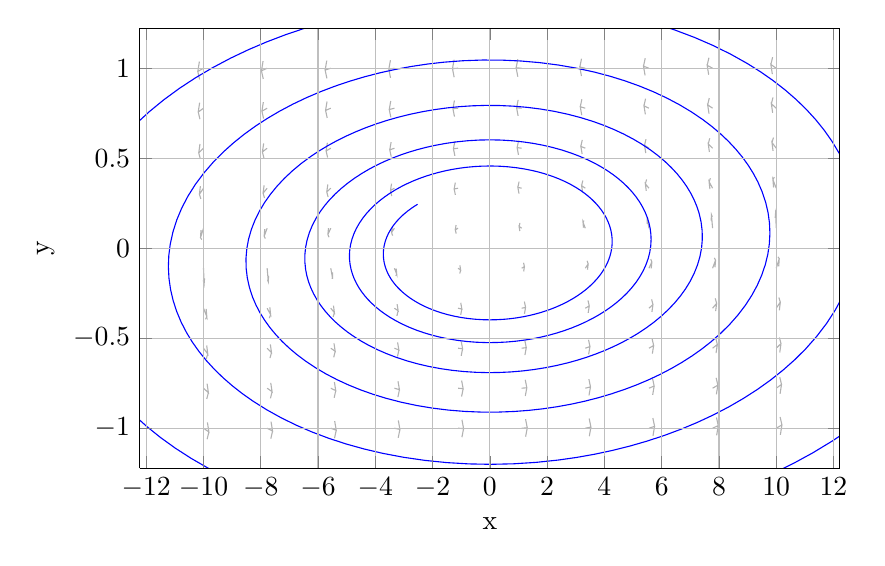
\begin{tikzpicture}

\begin{axis}[%
width=3.5in,
height=2.2in,
at={(0.866319in,1.696914in)},
scale only axis,
unbounded coords=jump,
separate axis lines,
every outer x axis line/.append style={black},
every x tick label/.append style={font=\color{black}},
xmin=-12.2222222222222,
xmax=12.2222222222222,
xlabel={x},
xmajorgrids,
every outer y axis line/.append style={black},
every y tick label/.append style={font=\color{black}},
ymin=-1.22222222222222,
ymax=1.22222222222222,
ylabel={y},
ymajorgrids,
every outer z axis line/.append style={black},
every z tick label/.append style={font=\color{black}},
zmin=-1,
zmax=1,
view={0}{90}
]
\addplot [color=white!70!black,solid,forget plot]
  table[row sep=crcr]{%
-10	-1\\
-9.81241194585928	-1.02056435585844\\
-9.86354727313689	-0.967498035565731\\
-9.81241194585928	-1.02056435585844\\
-9.87382945106611	-1.06129206263609\\
nan	0\\
-10	-0.777777777777778\\
-9.82958536756474	-0.802476346039514\\
-9.87453511522989	-0.752463117452179\\
-9.82958536756474	-0.802476346039514\\
-9.88688439936075	-0.837670433669807\\
nan	0\\
-10	-0.555555555555556\\
-9.85148358196474	-0.587306416934181\\
-9.88810079203066	-0.540652054011778\\
-9.85148358196474	-0.587306416934181\\
-9.90397622271997	-0.614910263029409\\
nan	0\\
-10	-0.333333333333333\\
-9.88446219903126	-0.380389184936132\\
-9.90735957642118	-0.337387979213108\\
-9.88446219903126	-0.380389184936132\\
-9.93088750222258	-0.395156879697477\\
nan	0\\
-10	-0.111111111111111\\
-9.97935536744191	-0.199672451922752\\
-9.96340842200643	-0.167942891539737\\
-9.97935536744191	-0.199672451922752\\
-10.0076890924122	-0.178265207818783\\
nan	0\\
-10	0.111111111111111\\
-10.1051566362561	0.0582449661940668\\
-10.06039310915	0.0478156506051543\\
-10.1051566362561	0.0582449661940668\\
-10.0868261816085	0.100393968733206\\
nan	0\\
-10	0.333333333333333\\
-10.1429235188413	0.299395502359456\\
-10.0915620054455	0.273845971941289\\
-10.1429235188413	0.299395502359456\\
-10.1085309209324	0.34530773136195\\
nan	0\\
-10	0.555555555555555\\
-10.1663153217761	0.529704325960978\\
-10.1099579178447	0.495880864395318\\
-10.1663153217761	0.529704325960978\\
-10.1228835326419	0.579038525283385\\
nan	0\\
-10	0.777777777777778\\
-10.1842555048727	0.756490782015734\\
-10.1236571044704	0.716813004526161\\
-10.1842555048727	0.756490782015734\\
-10.1343006023514	0.808940756962533\\
nan	0\\
-10	1\\
-10.1991602309428	0.981691466175508\\
-10.1348350282039	0.937393968587151\\
-10.1991602309428	0.981691466175508\\
-10.1439892951161	1.03697408405856\\
nan	0\\
-7.77777777777778	-1\\
-7.58854648285336	-1.01579673079962\\
-7.64136668863078	-0.963749887828626\\
-7.58854648285336	-1.01579673079962\\
-7.64926505403059	-1.05836553529084\\
nan	0\\
-7.77777777777778	-0.777777777777778\\
-7.6052640385214	-0.796689610627632\\
-7.65229020208585	-0.747887625958583\\
-7.6052640385214	-0.796689610627632\\
-7.66174611851078	-0.834144495586769\\
nan	0\\
-7.77777777777778	-0.555555555555556\\
-7.62624106257134	-0.57974393076523\\
-7.66565498333085	-0.534603239400719\\
-7.62624106257134	-0.57974393076523\\
-7.67774917093569	-0.610371597003936\\
nan	0\\
-7.77777777777778	-0.333333333333333\\
-7.65642428325531	-0.368944738617867\\
-7.68392748029092	-0.32792294340189\\
-7.65642428325531	-0.368944738617867\\
-7.70173318293318	-0.388599690663124\\
nan	0\\
-7.77777777777778	-0.111111111111111\\
-7.73599401236168	-0.187002745234794\\
-7.72955623345559	-0.153789313643665\\
-7.73599401236168	-0.187002745234794\\
-7.76750205051743	-0.174681196351713\\
nan	0\\
-7.77777777777778	0.111111111111111\\
-7.88119146430226	0.0662767369211356\\
-7.83895876479742	0.0538736275470088\\
-7.88119146430226	0.0662767369211356\\
-7.86137595189241	0.105580470809248\\
nan	0\\
-7.77777777777778	0.333333333333333\\
-7.91930735036248	0.305924850843073\\
-7.86999635796451	0.278765002443974\\
-7.91930735036248	0.305924850843073\\
-7.88370059920964	0.349529788736328\\
nan	0\\
-7.77777777777778	0.555555555555555\\
-7.94285876749928	0.534974090659561\\
-7.88818910435883	0.499878282697984\\
-7.94285876749928	0.534974090659561\\
-7.89847983680683	0.582418777558734\\
nan	0\\
-7.77777777777778	0.777777777777778\\
-7.96093376981838	0.760940492243617\\
-7.90177765082266	0.720202679893716\\
-7.96093376981838	0.760940492243617\\
-7.91019629358974	0.811780675914015\\
nan	0\\
-7.77777777777778	1\\
-7.97594664526146	0.985572129132925\\
-7.91288901729959	0.940358273522127\\
-7.97594664526146	0.985572129132925\\
-7.92010295273312	1.03944270726397\\
nan	0\\
-5.55555555555556	-1\\
-5.36478754435193	-1.01114168970936\\
-5.41923252528567	-0.960107179995643\\
-5.36478754435193	-1.01114168970936\\
-5.42480337014035	-1.05549118559746\\
nan	0\\
-5.55555555555556	-0.777777777777778\\
-5.38111717280357	-0.791071359758572\\
-5.43012529213397	-0.743473689476337\\
-5.38111717280357	-0.791071359758572\\
-5.43677208312436	-0.830692880852331\\
nan	0\\
-5.55555555555556	-0.555555555555556\\
-5.40134491418156	-0.572460909795196\\
-5.44338176803385	-0.528836643179804\\
-5.40134491418156	-0.572460909795196\\
-5.45183444515367	-0.605941963866804\\
nan	0\\
-5.55555555555556	-0.333333333333333\\
-5.42940822002481	-0.357961864284279\\
-5.4610952879463	-0.319036471116309\\
-5.42940822002481	-0.357961864284279\\
-5.47340955342177	-0.382110138881682\\
nan	0\\
-5.55555555555556	-0.111111111111111\\
-5.49219165581084	-0.167585175054708\\
-5.49708230974836	-0.13480198093545\\
-5.49219165581084	-0.167585175054708\\
-5.52531934172015	-0.166483930807808\\
nan	0\\
-5.55555555555556	0.111111111111111\\
-5.65702691981853	0.0758535140774167\\
-5.61777111128121	0.0610629521217819\\
-5.65702691981853	0.0758535140774167\\
-5.63539990979806	0.111798634253268\\
nan	0\\
-5.55555555555556	0.333333333333333\\
-5.69549479662779	0.312987412851764\\
-5.64842654418572	0.284106378728178\\
-5.69549479662779	0.312987412851764\\
-5.65859950442651	0.354075999264293\\
nan	0\\
-5.55555555555556	0.555555555555555\\
-5.71927934431476	0.540504646495139\\
-5.6663994804219	0.504088972023462\\
-5.71927934431476	0.540504646495139\\
-5.67392493495211	0.585950866403066\\
nan	0\\
-5.55555555555556	0.777777777777778\\
-5.73752955813875	0.76554669815799\\
-5.67987958745885	0.723722521398127\\
-5.73752955813875	0.76554669815799\\
-5.68599512726874	0.814709522689726\\
nan	0\\
-5.55555555555556	1\\
-5.75267374583829	0.989558311776526\\
-5.6909278666976	0.943411270672884\\
-5.75267374583829	0.989558311776526\\
-5.69614871080934	1.04197036581425\\
nan	0\\
-3.33333333333333	-1\\
-3.14112720121187	-1.00660003200747\\
-3.19713903284644	-0.956568489374861\\
-3.14112720121187	-1.00660003200747\\
-3.20043904885017	-1.05267155543559\\
nan	0\\
-3.33333333333333	-0.777777777777778\\
-3.15712878001146	-0.785624668790538\\
-3.20802842325483	-0.739219463156243\\
-3.15712878001146	-0.785624668790538\\
-3.21195186876122	-0.827321739817177\\
nan	0\\
-3.33333333333333	-0.555555555555556\\
-3.17675451149172	-0.565472721149544\\
-3.22124886664571	-0.523352866010944\\
-3.17675451149172	-0.565472721149544\\
-3.2262074494427	-0.60164227693175\\
nan	0\\
-3.33333333333333	-0.333333333333333\\
-3.20326704106137	-0.347591861317543\\
-3.23872229674691	-0.310797729854289\\
-3.20326704106137	-0.347591861317543\\
-3.24585156073901	-0.375830875990272\\
nan	0\\
-3.33333333333333	-0.111111111111111\\
-3.25322389641798	-0.143737816344082\\
-3.26910005118434	-0.113922445545352\\
-3.25322389641798	-0.143737816344082\\
-3.28541340380083	-0.153977164003029\\
nan	0\\
-3.33333333333333	0.111111111111111\\
-3.43243096649183	0.0875799333783673\\
-3.39681888211109	0.0698648784085666\\
-3.43243096649183	0.0875799333783673\\
-3.40858447097747	0.119413694987814\\
nan	0\\
-3.33333333333333	0.333333333333333\\
-3.47142332485981	0.320638904989292\\
-3.42682272031586	0.289924735610884\\
-3.47142332485981	0.320638904989292\\
-3.43316993448788	0.358969731374125\\
nan	0\\
-3.33333333333333	0.555555555555555\\
-3.49555527909082	0.546309329973755\\
-3.44457713896812	0.508527711208924\\
-3.49555527909082	0.546309329973755\\
-3.44920025175902	0.589638684087667\\
nan	0\\
-3.33333333333333	0.777777777777778\\
-3.51403282093641	0.770314352070681\\
-3.45795711822871	0.727378507882042\\
-3.51403282093641	0.770314352070681\\
-3.46168883108226	0.817728251683579\\
nan	0\\
-3.33333333333333	1\\
-3.52933604019161	0.99365235096644\\
-3.46894831587574	0.946555968961938\\
-3.52933604019161	0.99365235096644\\
-3.47212214039252	1.04455732239108\\
nan	0\\
-1.11111111111111	-1\\
-0.917557876910838	-1.00217177839591\\
-0.975080902571942	-0.953131936327069\\
-0.917557876910838	-1.00217177839591\\
-0.976166791769897	-1.04990855342721\\
nan	0\\
-1.11111111111111	-0.777777777777778\\
-0.933283653772106	-0.78035043854192\\
-0.985988725782772	-0.735121775977926\\
-0.933283653772106	-0.78035043854192\\
-0.987275056164843	-0.824035504647428\\
nan	0\\
-1.11111111111111	-0.555555555555556\\
-0.952431041938794	-0.558785881461918\\
-0.999227481213899	-0.51814676639693\\
-0.952431041938794	-0.558785881461918\\
-1.00084264416708	-0.597486800983088\\
nan	0\\
-1.11111111111111	-0.333333333333333\\
-0.977842822405366	-0.337909539936786\\
-1.01667925736623	-0.303219605779314\\
-0.977842822405366	-0.337909539936786\\
-1.01896736066795	-0.369853750132186\\
nan	0\\
-1.11111111111111	-0.111111111111111\\
-1.02092818095136	-0.120997422244607\\
-1.04551148221591	-0.0954857963646205\\
-1.02092818095136	-0.120997422244607\\
-1.05045463778266	-0.140577261444496\\
nan	0\\
-1.11111111111111	0.111111111111111\\
-1.20685736361098	0.102309286097334\\
-1.17593303160757	0.0810132704764999\\
-1.20685736361098	0.102309286097334\\
-1.18033394411446	0.128886396726434\\
nan	0\\
-1.11111111111111	0.333333333333333\\
-1.24701179771454	0.328932119310293\\
-1.20514128822775	0.296277311866348\\
-1.24701179771454	0.328932119310293\\
-1.20734189523927	0.364227655168063\\
nan	0\\
-1.11111111111111	0.555555555555555\\
-1.27166140789588	0.55239996184541\\
-1.22270742043291	0.513209065762261\\
-1.27166140789588	0.55239996184541\\
-1.22428521728799	0.593484214154647\\
nan	0\\
-1.11111111111111	0.777777777777778\\
-1.29043246978954	0.775247777514248\\
-1.23600356212013	0.731176437923701\\
-1.29043246978954	0.775247777514248\\
-1.23726856225189	0.820837117262913\\
nan	0\\
-1.11111111111111	1\\
-1.30592761362348	0.997856285321944\\
-1.24694673420026	0.949795274097268\\
-1.30592761362348	0.997856285321944\\
-1.24801859153928	1.04720352535345\\
nan	0\\
1.11111111111111	-1\\
1.30592761362348	-0.997856285321944\\
1.24694673420026	-0.949795274097268\\
1.30592761362348	-0.997856285321944\\
1.24801859153928	-1.04720352535345\\
nan	0\\
1.11111111111111	-0.777777777777778\\
1.29043246978954	-0.775247777514249\\
1.23600356212013	-0.731176437923701\\
1.29043246978954	-0.775247777514249\\
1.23726856225189	-0.820837117262914\\
nan	0\\
1.11111111111111	-0.555555555555556\\
1.27166140789588	-0.55239996184541\\
1.22270742043291	-0.513209065762261\\
1.27166140789588	-0.55239996184541\\
1.22428521728799	-0.593484214154647\\
nan	0\\
1.11111111111111	-0.333333333333333\\
1.24701179771454	-0.328932119310293\\
1.20514128822775	-0.296277311866348\\
1.24701179771454	-0.328932119310293\\
1.20734189523927	-0.364227655168063\\
nan	0\\
1.11111111111111	-0.111111111111111\\
1.20685736361098	-0.102309286097334\\
1.17593303160757	-0.0810132704764999\\
1.20685736361098	-0.102309286097334\\
1.18033394411446	-0.128886396726434\\
nan	0\\
1.11111111111111	0.111111111111111\\
1.02092818095136	0.120997422244607\\
1.04551148221591	0.0954857963646205\\
1.02092818095136	0.120997422244607\\
1.05045463778266	0.140577261444496\\
nan	0\\
1.11111111111111	0.333333333333333\\
0.977842822405366	0.337909539936786\\
1.01667925736623	0.303219605779314\\
0.977842822405366	0.337909539936786\\
1.01896736066795	0.369853750132186\\
nan	0\\
1.11111111111111	0.555555555555555\\
0.952431041938794	0.558785881461917\\
0.999227481213899	0.51814676639693\\
0.952431041938794	0.558785881461917\\
1.00084264416708	0.597486800983088\\
nan	0\\
1.11111111111111	0.777777777777778\\
0.933283653772106	0.780350438541919\\
0.985988725782772	0.735121775977926\\
0.933283653772106	0.780350438541919\\
0.987275056164843	0.824035504647428\\
nan	0\\
1.11111111111111	1\\
0.917557876910838	1.00217177839591\\
0.975080902571942	0.953131936327069\\
0.917557876910838	1.00217177839591\\
0.976166791769897	1.04990855342721\\
nan	0\\
3.33333333333333	-1\\
3.52933604019161	-0.99365235096644\\
3.46894831587574	-0.946555968961938\\
3.52933604019161	-0.99365235096644\\
3.47212214039252	-1.04455732239108\\
nan	0\\
3.33333333333333	-0.777777777777778\\
3.51403282093641	-0.770314352070682\\
3.45795711822871	-0.727378507882042\\
3.51403282093641	-0.770314352070682\\
3.46168883108226	-0.817728251683579\\
nan	0\\
3.33333333333333	-0.555555555555556\\
3.49555527909082	-0.546309329973756\\
3.44457713896812	-0.508527711208924\\
3.49555527909082	-0.546309329973756\\
3.44920025175902	-0.589638684087667\\
nan	0\\
3.33333333333333	-0.333333333333333\\
3.47142332485981	-0.320638904989292\\
3.42682272031586	-0.289924735610884\\
3.47142332485981	-0.320638904989292\\
3.43316993448788	-0.358969731374125\\
nan	0\\
3.33333333333333	-0.111111111111111\\
3.43243096649183	-0.0875799333783673\\
3.39681888211109	-0.0698648784085666\\
3.43243096649183	-0.0875799333783673\\
3.40858447097747	-0.119413694987814\\
nan	0\\
3.33333333333333	0.111111111111111\\
3.25322389641798	0.143737816344082\\
3.26910005118434	0.113922445545352\\
3.25322389641798	0.143737816344082\\
3.28541340380083	0.153977164003029\\
nan	0\\
3.33333333333333	0.333333333333333\\
3.20326704106137	0.347591861317543\\
3.23872229674691	0.310797729854289\\
3.20326704106137	0.347591861317543\\
3.24585156073901	0.375830875990272\\
nan	0\\
3.33333333333333	0.555555555555555\\
3.17675451149172	0.565472721149543\\
3.22124886664571	0.523352866010944\\
3.17675451149172	0.565472721149543\\
3.2262074494427	0.60164227693175\\
nan	0\\
3.33333333333333	0.777777777777778\\
3.15712878001147	0.785624668790538\\
3.20802842325484	0.739219463156243\\
3.15712878001147	0.785624668790538\\
3.21195186876122	0.827321739817177\\
nan	0\\
3.33333333333333	1\\
3.14112720121187	1.00660003200747\\
3.19713903284644	0.956568489374861\\
3.14112720121187	1.00660003200747\\
3.20043904885018	1.05267155543559\\
nan	0\\
5.55555555555556	-1\\
5.75267374583829	-0.989558311776526\\
5.6909278666976	-0.943411270672884\\
5.75267374583829	-0.989558311776526\\
5.69614871080934	-1.04197036581425\\
nan	0\\
5.55555555555556	-0.777777777777778\\
5.73752955813876	-0.76554669815799\\
5.67987958745885	-0.723722521398127\\
5.73752955813876	-0.76554669815799\\
5.68599512726874	-0.814709522689726\\
nan	0\\
5.55555555555556	-0.555555555555556\\
5.71927934431477	-0.540504646495139\\
5.6663994804219	-0.504088972023462\\
5.71927934431477	-0.540504646495139\\
5.67392493495211	-0.585950866403066\\
nan	0\\
5.55555555555556	-0.333333333333333\\
5.69549479662779	-0.312987412851765\\
5.64842654418573	-0.284106378728178\\
5.69549479662779	-0.312987412851765\\
5.65859950442651	-0.354075999264293\\
nan	0\\
5.55555555555556	-0.111111111111111\\
5.65702691981853	-0.0758535140774167\\
5.61777111128121	-0.0610629521217819\\
5.65702691981853	-0.0758535140774167\\
5.63539990979806	-0.111798634253268\\
nan	0\\
5.55555555555556	0.111111111111111\\
5.49219165581084	0.167585175054708\\
5.49708230974836	0.13480198093545\\
5.49219165581084	0.167585175054708\\
5.52531934172016	0.166483930807808\\
nan	0\\
5.55555555555556	0.333333333333333\\
5.42940822002481	0.357961864284279\\
5.4610952879463	0.319036471116309\\
5.42940822002481	0.357961864284279\\
5.47340955342177	0.382110138881681\\
nan	0\\
5.55555555555556	0.555555555555555\\
5.40134491418156	0.572460909795196\\
5.44338176803385	0.528836643179804\\
5.40134491418156	0.572460909795196\\
5.45183444515367	0.605941963866804\\
nan	0\\
5.55555555555556	0.777777777777778\\
5.38111717280357	0.791071359758572\\
5.43012529213397	0.743473689476337\\
5.38111717280357	0.791071359758572\\
5.43677208312436	0.830692880852331\\
nan	0\\
5.55555555555556	1\\
5.36478754435193	1.01114168970936\\
5.41923252528568	0.960107179995643\\
5.36478754435193	1.01114168970936\\
5.42480337014036	1.05549118559746\\
nan	0\\
7.77777777777778	-1\\
7.97594664526146	-0.985572129132925\\
7.91288901729959	-0.940358273522127\\
7.97594664526146	-0.985572129132925\\
7.92010295273312	-1.03944270726397\\
nan	0\\
7.77777777777778	-0.777777777777778\\
7.96093376981838	-0.760940492243617\\
7.90177765082266	-0.720202679893716\\
7.96093376981838	-0.760940492243617\\
7.91019629358974	-0.811780675914015\\
nan	0\\
7.77777777777778	-0.555555555555556\\
7.94285876749928	-0.534974090659561\\
7.88818910435883	-0.499878282697984\\
7.94285876749928	-0.534974090659561\\
7.89847983680683	-0.582418777558735\\
nan	0\\
7.77777777777778	-0.333333333333333\\
7.91930735036249	-0.305924850843073\\
7.86999635796451	-0.278765002443974\\
7.91930735036249	-0.305924850843073\\
7.88370059920964	-0.349529788736328\\
nan	0\\
7.77777777777778	-0.111111111111111\\
7.88119146430226	-0.0662767369211356\\
7.83895876479742	-0.0538736275470088\\
7.88119146430226	-0.0662767369211356\\
7.86137595189241	-0.105580470809248\\
nan	0\\
7.77777777777778	0.111111111111111\\
7.73599401236168	0.187002745234794\\
7.72955623345559	0.153789313643665\\
7.73599401236168	0.187002745234794\\
7.76750205051743	0.174681196351713\\
nan	0\\
7.77777777777778	0.333333333333333\\
7.65642428325531	0.368944738617867\\
7.68392748029092	0.32792294340189\\
7.65642428325531	0.368944738617867\\
7.70173318293319	0.388599690663124\\
nan	0\\
7.77777777777778	0.555555555555555\\
7.62624106257134	0.579743930765229\\
7.66565498333086	0.534603239400719\\
7.62624106257134	0.579743930765229\\
7.67774917093569	0.610371597003936\\
nan	0\\
7.77777777777778	0.777777777777778\\
7.60526403852141	0.796689610627632\\
7.65229020208585	0.747887625958582\\
7.60526403852141	0.796689610627632\\
7.66174611851078	0.834144495586769\\
nan	0\\
7.77777777777778	1\\
7.58854648285336	1.01579673079962\\
7.64136668863078	0.963749887828626\\
7.58854648285336	1.01579673079962\\
7.64926505403059	1.05836553529084\\
nan	0\\
10	-1\\
10.1991602309428	-0.981691466175508\\
10.1348350282039	-0.937393968587151\\
10.1991602309428	-0.981691466175508\\
10.1439892951161	-1.03697408405856\\
nan	0\\
10	-0.777777777777778\\
10.1842555048727	-0.756490782015735\\
10.1236571044704	-0.716813004526161\\
10.1842555048727	-0.756490782015735\\
10.1343006023514	-0.808940756962534\\
nan	0\\
10	-0.555555555555556\\
10.1663153217761	-0.529704325960978\\
10.1099579178447	-0.495880864395318\\
10.1663153217761	-0.529704325960978\\
10.1228835326419	-0.579038525283385\\
nan	0\\
10	-0.333333333333333\\
10.1429235188413	-0.299395502359456\\
10.0915620054455	-0.273845971941289\\
10.1429235188413	-0.299395502359456\\
10.1085309209324	-0.34530773136195\\
nan	0\\
10	-0.111111111111111\\
10.1051566362561	-0.0582449661940668\\
10.06039310915	-0.0478156506051543\\
10.1051566362561	-0.0582449661940668\\
10.0868261816085	-0.100393968733206\\
nan	0\\
10	0.111111111111111\\
9.97935536744191	0.199672451922752\\
9.96340842200643	0.167942891539737\\
9.97935536744191	0.199672451922752\\
10.0076890924122	0.178265207818783\\
nan	0\\
10	0.333333333333333\\
9.88446219903126	0.380389184936132\\
9.90735957642118	0.337387979213108\\
9.88446219903126	0.380389184936132\\
9.93088750222258	0.395156879697477\\
nan	0\\
10	0.555555555555555\\
9.85148358196474	0.587306416934181\\
9.88810079203066	0.540652054011777\\
9.85148358196474	0.587306416934181\\
9.90397622271997	0.614910263029409\\
nan	0\\
10	0.777777777777778\\
9.82958536756474	0.802476346039514\\
9.87453511522989	0.752463117452179\\
9.82958536756474	0.802476346039514\\
9.88688439936075	0.837670433669807\\
nan	0\\
10	1\\
9.81241194585928	1.02056435585844\\
9.86354727313689	0.967498035565731\\
9.81241194585928	1.02056435585844\\
9.87382945106611	1.06129206263609\\
nan	0\\
};
\addplot3 [color=blue,solid]
 table[row sep=crcr] {%
-2.52463885513703	0.243956531381681	0\\
-2.54953737148386	0.241573134930288	0.00093941572513655\\
-2.57423134515417	0.239166444273283	0.0018788314502731\\
-2.59871842594613	0.236736652744317	0.00281824717540965\\
-2.62299628079593	0.234283955824116	0.0037576629005462\\
-2.64706259377769	0.231808551140481	0.00469707862568275\\
-2.67091506610354	0.229310638468288	0.0056364943508193\\
-2.69455141612358	0.226790419729493	0.00657591007595585\\
-2.71796937932587	0.224248098993123	0.0075153258010924\\
-2.87093750186743	0.206430280681934	0.0138892881847653\\
-3.01308353242483	0.187671510045082	0.0202632505684381\\
-3.14374765124357	0.168043579318806	0.026637212952111\\
-3.26232466213577	0.147621573462762	0.0330111753357839\\
-3.36826399248022	0.126483870160022	0.0393851377194568\\
-3.46106969322239	0.104712139817074	0.0457591001031296\\
-3.54030043887437	0.0823913455638228	0.0521330624868025\\
-3.60556952751492	0.0596097432535889	0.0585070248704754\\
-3.65674854854113	0.0363468895394741	0.0649109798562709\\
-3.69319267624266	0.0128026281744376	0.0713149348420665\\
-3.71465353409658	-0.0109262044812335	0.077718889827862\\
-3.7209504564399	-0.0347426366653714	0.0841228448136576\\
-3.71197048846954	-0.058549561213928	0.0905267997994531\\
-3.68766838624232	-0.0822497355609748	0.0969307547852487\\
-3.64806661667503	-0.105745781738703	0.103334709771044\\
-3.59325535754434	-0.128940186377423	0.10973866475684\\
-3.53749851312201	-0.14753326109541	0.11495217130921\\
-3.47185230948046	-0.165810243656967	0.12016567786158\\
-3.39644856418335	-0.183719105734031	0.12537918441395\\
-3.31144648215976	-0.20120908967568	0.13059269096632\\
-3.21703265570418	-0.218230708508127	0.13580619751869\\
-3.11342106447648	-0.234735745934728	0.14101970407106\\
-3.00085307550193	-0.250677256335975	0.14623321062343\\
-2.8795974431712	-0.266009564769501	0.1514467171758\\
-2.73496906640253	-0.282284423132991	0.157241947558176\\
-2.5803964009829	-0.297692900951248	0.163037177940551\\
-2.41635155660908	-0.312177355604101	0.168832408322927\\
-2.24333786526468	-0.325683759822201	0.174627638705302\\
-2.06188988122023	-0.338161701687018	0.180422869087678\\
-1.87257338103308	-0.349564384630844	0.186218099470053\\
-1.6759853635475	-0.359848627436792	0.192013329852428\\
-1.47275404989459	-0.368974864238796	0.197808560234804\\
-1.24026992139891	-0.377702432745986	0.204238510846364\\
-1.00132286913168	-0.384915162046602	0.210668461457923\\
-0.756880311784414	-0.390572688852038	0.217098412069483\\
-0.507927242639707	-0.39464184138227	0.223528362681043\\
-0.255466229571245	-0.397096639365854	0.229958313292602\\
-0.000517415043803648	-0.397918294039927	0.236388263904162\\
0.255881483886752	-0.397095208150209	0.242818214515722\\
0.512675175573474	-0.394622975951	0.249248165127282\\
0.728051775887023	-0.391270089216833	0.254652781745618\\
0.942326705630462	-0.386756187228877	0.260057398363955\\
1.15485799175283	-0.381088613766554	0.265462014982292\\
1.36501198754741	-0.374278238980948	0.270866631600629\\
1.57216337265174	-0.366339459394804	0.276271248218966\\
1.77569515304762	-0.357290197902528	0.281675864837303\\
1.97499866106106	-0.347151903770187	0.28708048145564\\
2.16947355536236	-0.33594955263551	0.292485098073977\\
2.35623358732023	-0.323868243679008	0.297822949387578\\
2.53714879569578	-0.310805468894792	0.303160800701179\\
2.71166533402786	-0.296794005001333	0.30849865201478\\
2.8792510552048	-0.281869335907071	0.313836503328381\\
3.0393955114644	-0.266069652710418	0.319174354641982\\
3.19160995439394	-0.249435853699758	0.324512205955584\\
3.33542733493016	-0.232011544353442	0.329850057269185\\
3.47040230335928	-0.213843037339796	0.335187908582786\\
3.61416004235552	-0.192090168523607	0.341326815907968\\
3.74505296214502	-0.169493719262271	0.347465723233149\\
3.86249878011785	-0.146135404991408	0.353604630558331\\
3.96597306874113	-0.122099493172007	0.359743537883513\\
4.055009255559	-0.0974728032904351	0.365882445208694\\
4.12919862319264	-0.072344706858429	0.372021352533876\\
4.18819030934024	-0.0468071274131004	0.378160259859057\\
4.23169130677705	-0.0209545405169332	0.384299167184239\\
4.2580712590717	0.00333609511056443	0.390019732919852\\
4.27062401230471	0.0277387196872827	0.395740298655465\\
4.26923027485969	0.0521726547075702	0.401460864391079\\
4.25381984529303	0.0765575417634933	0.407181430126692\\
4.2243716123339	0.100813342544836	0.412901995862305\\
4.18091355488423	0.1248603388391	0.418622561597918\\
4.12352274201875	0.148619132531505	0.424343127333531\\
4.05232533298495	0.172010645604989	0.430063693069144\\
3.9787313005877	0.192140749170099	0.435075523518222\\
3.89479990435716	0.211876457286547	0.440087353967299\\
3.80069580327496	0.231165598145863	0.445099184416376\\
3.69660987515563	0.249957372712364	0.450111014865454\\
3.58275921664664	0.268202354723152	0.455122845314531\\
3.45938714322839	0.285852490688118	0.460134675763608\\
3.32676318921417	0.302861099889936	0.465146506212686\\
3.18518310775021	0.31918287438407	0.470158336661763\\
3.00795439468882	0.337410896808102	0.476042580715478\\
2.81936808959254	0.354563369136315	0.481926824769194\\
2.62002360626585	0.370573526666975	0.487811068822909\\
2.41055659059686	0.385379195936704	0.493695312876624\\
2.19163892055738	0.398922794720484	0.49957955693034\\
1.96397870620289	0.41115133203165	0.505463800984055\\
1.72832028967254	0.422016408121895	0.51134804503777\\
1.48544424518916	0.431474214481271	0.517232289091486\\
1.21036192340659	0.440221183032222	0.523717366640754\\
0.928597675959549	0.447163479368953	0.530202444190022\\
0.641318758376293	0.45225934008511	0.536687521739291\\
0.349708955064771	0.455475651364104	0.543172599288559\\
0.0549685793126407	0.456787948979118	0.549657676837828\\
-0.241685526712736	0.456180418293104	0.556142754387096\\
-0.539019991964293	0.453645894258782	0.562627831936365\\
-0.835784916515264	0.449185861418642	0.569112909485633\\
-1.0801310939543	0.444042666077613	0.574481366189135\\
-1.3225179323629	0.437592974688615	0.579849822892637\\
-1.56222532421052	0.429848916854006	0.585218279596139\\
-1.79854456138531	0.420826506262126	0.590586736299641\\
-2.03077833519408	0.410545640687297	0.595955193003143\\
-2.25824073636236	0.399030101989818	0.601323649706645\\
-2.48025725503432	0.386307556115973	0.606692106410146\\
-2.69616478077284	0.372409553098023	0.612060563113648\\
-2.90909737484152	0.357083617291038	0.617527736543755\\
-3.11434774240454	0.340614312495133	0.622994909973862\\
-3.31125140418673	0.323045641339808	0.628462083403968\\
-3.49917340591627	0.304424873187658	0.633929256834075\\
-3.6775083183247	0.284802544134369	0.639396430264182\\
-3.8456802371469	0.264232457008719	0.644863603694289\\
-4.00314278312111	0.24277168137258	0.650330777124395\\
-4.1493791019889	0.220480553520914	0.655797950554502\\
-4.30138347266504	0.194209297836297	0.662013312356874\\
-4.43757638684455	0.167041697254854	0.668228674159246\\
-4.55732215685077	0.139079292614893	0.674444035961618\\
-4.66005724091033	0.110426249090555	0.68065939776399\\
-4.74529024315323	0.0811893561918218	0.686874759566362\\
-4.81260191361277	0.0514780277645118	0.693090121368734\\
-4.86164514822559	0.0214043019902807	0.699305483171106\\
-4.89214498883165	-0.00891715861337908	0.705520844973478\\
-4.90345962977691	-0.0356155959869364	0.710970421242432\\
-4.90023965023054	-0.0623366841666692	0.716419997511386\\
-4.88241814227239	-0.0889998586991246	0.72186957378034\\
-4.84997435484199	-0.115525114799782	0.727319150049294\\
-4.8029336937386	-0.141833007353052	0.732768726318248\\
-4.74136772162114	-0.167844650912278	0.738218302587202\\
-4.66539415800825	-0.193481719699734	0.743667878856156\\
-4.57517687927826	-0.218666447606629	0.74911745512511\\
-4.48002780884107	-0.241313713763144	0.754118264957009\\
-4.37323505382051	-0.263456436462847	0.759119074788909\\
-4.25501424674027	-0.285036042603881	0.764119884620808\\
-4.12561022761644	-0.305995655072633	0.769120694452708\\
-3.98529704395749	-0.326280092743741	0.774121504284607\\
-3.83437795076429	-0.345835870480088	0.779122314116507\\
-3.67318541053011	-0.364611199132803	0.784123123948406\\
-3.50208109324059	-0.382555985541264	0.789123933780306\\
-3.2857589370373	-0.40279067879689	0.795083563795009\\
-3.05660320166021	-0.421698802355246	0.801043193809713\\
-2.81536781006231	-0.439204064421199	0.807002823824416\\
-2.56284797294821	-0.455235932834348	0.81296245383912\\
-2.29988018877408	-0.469729635069017	0.818922083853823\\
-2.02734224374768	-0.482626158234261	0.824881713868527\\
-1.74615321182836	-0.493872249073861	0.83084134388323\\
-1.45727345472705	-0.503420413966331	0.836800973897934\\
-1.13243096622625	-0.511898489576752	0.843343768968266\\
-0.800846502565246	-0.518230196439062	0.849886564038599\\
-0.463926513581075	-0.522373472657226	0.856429359108931\\
-0.123091691784856	-0.524296647442224	0.862972154179264\\
0.220223027638204	-0.523978441112045	0.869514949249596\\
0.564568466828807	-0.521407965091686	0.876057744319928\\
0.908481205253567	-0.516584721913158	0.882600539390261\\
1.25048357970502	-0.509518605215481	0.889143334460593\\
1.52685136182108	-0.502110892701279	0.894477071976976\\
1.80017017740532	-0.493237207586073	0.89981080949336\\
2.0696342615021	-0.482915674745765	0.905144547009743\\
2.33445299128273	-0.471168685433431	0.910478284526126\\
2.5938508860454	-0.458022897279325	0.91581202204251\\
2.84706760721524	-0.443509234290877	0.921145759558893\\
3.09335795834426	-0.427662886852689	0.926479497075276\\
3.33199188511143	-0.410523311726544	0.931813234591659\\
3.57296731548468	-0.391230423439519	0.937400006255398\\
3.80396052730072	-0.370618832041845	0.942986777919136\\
4.0241836855056	-0.348746821402461	0.948573549582874\\
4.23288851141038	-0.325676551678942	0.954160321246612\\
4.42936628269115	-0.301474059317501	0.959747092910351\\
4.61294783338905	-0.276209257052983	0.965333864574089\\
4.78300355391024	-0.249955933908872	0.970920636237827\\
4.93894339102594	-0.222791755197286	0.976507407901565\\
5.09695909764897	-0.191214261779277	0.982798072832153\\
5.2356469506793	-0.158702605364944	0.989088737762741\\
5.35432398752309	-0.125382248726769	0.995379402693329\\
5.45239668617473	-0.0913812425908319	1.00167006762392\\
5.52936096521684	-0.0568302256368078	1.0079607325545\\
5.58480218382025	-0.0218624244979693	1.01425139748509\\
5.61839514174403	0.0133863462388142	1.02054206241568\\
5.62990407933544	0.0487776840330781	1.02683272734627\\
5.62203885895981	0.0791744564792287	1.03223416376666\\
5.59770332674167	0.10948492986247	1.03763560018704\\
5.55688376384794	0.139618763786658	1.04303703660743\\
5.49961731935771	0.169486576154884	1.04843847302782\\
5.42599201026228	0.198999943169474	1.05383990944821\\
5.33614672146511	0.228071399331993	1.0592413458686\\
5.23027120578187	0.256614437443239	1.06464278228899\\
5.10860608394038	0.284543508603249	1.07004421870937\\
4.97633356131725	0.310863992906032	1.0752625459558\\
4.82987567839244	0.336457776915644	1.08048087320223\\
4.66956654150022	0.361250448835276	1.08569920044866\\
4.49577859503672	0.385170205660132	1.09091752769508\\
4.30892262145996	0.408147853177434	1.09613585494151\\
4.10944774128986	0.43011680596642	1.10135418218794\\
3.89784141310818	0.451013087398344	1.10657250943437\\
3.6746294335586	0.470775329636476	1.1117908366808\\
3.40108260051971	0.492262265885678	1.11786162768086\\
3.11350670569581	0.512047037949123	1.12393241868093\\
2.81289795512307	0.530044977352055	1.13000320968099\\
2.50029770423504	0.546178968513058	1.13607400068106\\
2.1767924578627	0.560379448744062	1.14214479168112\\
1.84351387023446	0.572584408250339	1.14821558268119\\
1.50163874497611	0.582739390130504	1.15428637368126\\
1.15238903511087	0.590797490376516	1.16035716468132\\
0.774401234740981	0.597020414278004	1.16681097735645\\
0.391018877244034	0.600787465808141	1.17326479003157\\
0.00383870456758495	0.602066497087122	1.17971860270669\\
-0.385536914574306	0.600836724898174	1.18617241538182\\
-0.775499984701076	0.597088730687549	1.19262622805694\\
-1.16443688356565	0.590824460564531	1.19908004073206\\
-1.55072836215446	0.582057225301431	1.20553385340719\\
-1.93274954468742	0.570811700333588	1.21198766608231\\
-2.23880098516255	0.559875774153527	1.21722994404303\\
-2.54010623989631	0.547347783612344	1.22247222200376\\
-2.83580043306064	0.533254693590891	1.22771449996448\\
-3.12503859556705	0.517627887513325	1.23295677792521\\
-3.40699566506663	0.50050316734712	1.23819905588593\\
-3.68086648595004	0.48192075360306	1.24344133384665\\
-3.94586580934751	0.461925285335244	1.24868361180738\\
-4.20122829312885	0.44056582014108	1.2539258897681\\
-4.46912041172518	0.415655585448098	1.25967044428071\\
-4.7235981794682	0.389244507514765	1.26541499879333\\
-4.9637309276595	0.361412881399265	1.27115955330594\\
-5.18864326647325	0.332245549745374	1.27690410781855\\
-5.3975150849562	0.301831902782459	1.28264866233117\\
-5.58958155102767	0.270265878325481	1.28839321684378\\
-5.76413311147957	0.237645961774991	1.29413777135639\\
-5.92051549197638	0.204075186117134	1.299882325869\\
-6.07250831957859	0.165714183359902	1.30627713805909\\
-6.20048224308383	0.12645675833523	1.31267195024917\\
-6.303746912819	0.0864611352388039	1.31906676243925\\
-6.38172526307845	0.0458876759251402	1.32546157462933\\
-6.43395351212402	0.00489887990758892	1.33185638681941\\
-6.46008116218502	-0.036340615641668	1.3382511990095\\
-6.45987099945826	-0.0776640358916159	1.34464601119958\\
-6.43319909410797	-0.118902468352409	1.35104082338966\\
-6.3906272033124	-0.153150048186647	1.35638059839411\\
-6.32959934844859	-0.187121762939165	1.36172037339856\\
-6.2501974584375	-0.220717763370481	1.36706014840301\\
-6.15255839005245	-0.253839774536682	1.37239992340746\\
-6.03687392791903	-0.286391095789431	1.37773969841192\\
-5.90339078451516	-0.318276600775966	1.38307947341637\\
-5.7524106001711	-0.349402737439093	1.38841924842082\\
-5.5842899430694	-0.379677528017196	1.39375902342527\\
-5.39484430476572	-0.409695163550463	1.39922544894041\\
-5.18833259126714	-0.438631352493332	1.40469187445556\\
-4.96529195461284	-0.466392450380913	1.4101582999707\\
-4.72630923654709	-0.492888968660615	1.41562472548585\\
-4.47202096851926	-0.518035574692146	1.42109115100099\\
-4.20311337168382	-0.54175109174751	1.42655757651614\\
-3.92032235690035	-0.563958499011011	1.43202400203128\\
-3.6244335247335	-0.584584931579251	1.43749042754643\\
-3.27323947734976	-0.606024609299606	1.44370391169096\\
-2.90745082944039	-0.625238112288525	1.4499173958355\\
-2.52841813561522	-0.642135840254608	1.45613087998003\\
-2.13753787772163	-0.65663834524016	1.46234436412456\\
-1.73625246484452	-0.668676331621196	1.4685578482691\\
-1.3260502333063	-0.678190656107438	1.47477133241363\\
-0.908465446666925	-0.685132327742314	1.48098481655816\\
-0.485078295723864	-0.68946250790296	1.48719830070269\\
-0.0823042790979306	-0.691125916687632	1.49305234726862\\
0.322838983398461	-0.690424975978886	1.49890639383454\\
0.728950576029773	-0.68734849164594	1.50476044040046\\
1.13463394379846	-0.681893994450682	1.51061448696638\\
1.53849689244495	-0.674067740047676	1.5164685335323\\
1.93915158844768	-0.663884708984158	1.52232258009822\\
2.33521455902307	-0.651368606700039	1.52817662666414\\
2.72530669212553	-0.636551863527901	1.53403067323006\\
3.05568570915643	-0.621965493416638	1.53907616331742\\
3.37974409875082	-0.605727979124974	1.54412165340477\\
3.69661443656387	-0.587873337944721	1.54916714349213\\
4.00545182470155	-0.568439783073034	1.55421263357949\\
4.30543389172056	-0.547469723612406	1.55925812366684\\
4.59576079262842	-0.525009764570673	1.5643036137542\\
4.87565520888341	-0.501110706861014	1.56934910384156\\
5.14436234839459	-0.475827547301945	1.57439459392892\\
5.44177656662719	-0.444766634101765	1.58026116104664\\
5.72197069084942	-0.412010814855438	1.58612772816436\\
5.98386252380373	-0.377665150115029	1.59199429528208\\
6.22644303097867	-0.34183992843919	1.5978608623998\\
6.44877634060887	-0.304650666393161	1.60372742951752\\
6.64999974367505	-0.266218108548766	1.60959399663524\\
6.82932369390403	-0.226668227484417	1.61546056375296\\
6.9860318077687	-0.186132223785111	1.62132713087068\\
7.13194739077126	-0.140416425258992	1.62780084306816\\
7.24875372667252	-0.0938486153146721	1.63427455526565\\
7.33575866567383	-0.0466226750675951	1.64074826746313\\
7.39240927445341	0.0010659401770956	1.64722197966061\\
7.41829183616633	0.0490202009245581	1.6536956918581\\
7.41313185044453	0.0970415034902513	1.66016940405558\\
7.37679403339684	0.144929669999935	1.66664311625307\\
7.30928231760891	0.192482948389671	1.67311682845055\\
7.23096001557147	0.230989216768199	1.67841189481341\\
7.13196032206585	0.269026831837128	1.68370696117628\\
7.01246000748691	0.306485059062228	1.68900202753914\\
6.8726956951557	0.343255358250338	1.69429709390201\\
6.71296386131948	0.379231383549362	1.69959216026487\\
6.53362083515169	0.414308983448276	1.70488722662773\\
6.33508279875199	0.448386200777122	1.7101822929906\\
6.11782578714619	0.481363272707012	1.71547735935346\\
5.86697312913968	0.515099773697118	1.72110534075919\\
5.59625394206166	0.547369609859529	1.72673332216492\\
5.30643181102717	0.578060714849136	1.73236130357065\\
4.99833057370882	0.607066895048946	1.73798928497638\\
4.67283432033674	0.634287829570081	1.74361726638211\\
4.33088739369865	0.659629070251776	1.74924524778785\\
3.97349438913982	0.683002041661383	1.75487322919358\\
3.60172015456305	0.704324041094369	1.76050121059931\\
3.16870830355461	0.725717612934557	1.7668175621919\\
2.72060632280285	0.744330025211493	1.7731339137845\\
2.25914395195512	0.76006771268084	1.7794502653771\\
1.78609636241945	0.772850039588954	1.78576661696969\\
1.3032841573646	0.782609299672881	1.79208296856229\\
0.812573371720026	0.789290716160358	1.79839932015489\\
0.315875472175895	0.792852441769813	1.80471567174748\\
-0.184852642816931	0.793265558710366	1.81103202334008\\
-0.620397685527848	0.791063521530621	1.81650420954154\\
-1.05618854490361	0.786477623949286	1.821976395743\\
-1.4908995674507	0.779509196725716	1.82744858194445\\
-1.92321480455029	0.770167109374572	1.83292076814591\\
-2.35182801245825	0.758467770165823	1.83839295434737\\
-2.77544265230519	0.744435126124746	1.84386514054882\\
-3.19277189009639	0.728100663031926	1.84933732675028\\
-3.60253859671186	0.709503405423253	1.85480951295174\\
-3.97069740335034	0.690492399221125	1.85982921843037\\
-4.33046523087744	0.669654173747204	1.86484892390901\\
-4.68088230970327	0.647033283435818	1.86986862938765\\
-5.02101721595129	0.622678833292475	1.87488833486628\\
-5.34996687145831	0.59664447889386	1.87990804034492\\
-5.66685654377449	0.568988426387834	1.88492774582356\\
-5.97083984616335	0.539773432493437	1.88994745130219\\
-6.26109873760173	0.509066804500887	1.89496715678083\\
-6.58737753736975	0.470701305130512	1.90093736618176\\
-6.89185643833642	0.430452097139635	1.90690757558269\\
-7.17330004719471	0.388454287764456	1.91287778498361\\
-7.43056779971555	0.344848829155739	1.91884799438454\\
-7.66261396074784	0.29978251837881	1.92481820378547\\
-7.86848762421841	0.25340799741356	1.9307884131864\\
-8.04733271313209	0.20588375315444	1.93675862258732\\
-8.19838797957162	0.157374117410465	1.94272883198825\\
-8.32839419185422	0.10461078108421	1.94911156313784\\
-8.42514137044121	0.0511219312172363	1.95549429428743\\
-8.4880118726577	-0.00287448250690836	1.96187702543702\\
-8.5165404668062	-0.0571598037156272	1.96825975658661\\
-8.51041433216656	-0.111514669347273	1.9746424877362\\
-8.46947305899601	-0.165719009651147	1.9810252188858\\
-8.39370864852913	-0.219552048187502	1.98740795003539\\
-8.28326551297786	-0.272792301827539	1.99379068118498\\
-8.16727856612876	-0.315761280455246	1.99901330727899\\
-8.02843918129436	-0.358065697314853	2.004235933373\\
-7.86701759282634	-0.399585039926258	2.00945855946701\\
-7.68334779370324	-0.440201556102759	2.01468118556103\\
-7.47782753553043	-0.479800253951053	2.01990381165504\\
-7.2509183285401	-0.518268901871232	2.02512643774905\\
-7.00314544159129	-0.555498028556786	2.03034906384306\\
-6.73509790216988	-0.591380922994606	2.03557168993707\\
-6.41770382576029	-0.629162143560262	2.04131459829506\\
-6.07749105013688	-0.665056372723018	2.04705750665304\\
-5.71547364078329	-0.698932441940981	2.05280041501102\\
-5.33273659773053	-0.730666956214703	2.058543323369\\
-4.93043585555696	-0.760144294087184	2.06428623172698\\
-4.5097982833883	-0.787256607643872	2.07002914008496\\
-4.07212168489767	-0.81190382251266	2.07577204844295\\
-3.61877479830549	-0.83399363786389	2.08151495680093\\
-3.09742533284057	-0.855473063250543	2.08790756963223\\
-2.56043944450083	-0.873571541115752	2.09430018246353\\
-2.00995802777812	-0.888191605965933	2.10069279529483\\
-1.44816626644943	-0.8992517300686	2.10708540812613\\
-0.877293633576849	-0.906686323452369	2.11347802095743\\
-0.299613891507601	-0.910445733906954	2.11987063378873\\
0.282554908125965	-0.910496246983171	2.12626324662003\\
0.866850424406395	-0.906820085992938	2.13265585945134\\
1.36218192190706	-0.900779381861014	2.13807618199253\\
1.85587718558672	-0.892058379435891	2.14349650453373\\
2.34645312029365	-0.880669088272393	2.14891682707493\\
2.83244317271144	-0.866631746304842	2.15433714961612\\
3.31239733135896	-0.849974819847056	2.15975747215732\\
3.78488212659037	-0.830735003592351	2.16517779469851\\
4.24848063059511	-0.80895722061354	2.17059811723971\\
4.70179245739797	-0.784694622362931	2.17601843978091\\
5.12914999854503	-0.758920565745572	2.18126085562998\\
5.54436499810676	-0.730937609314474	2.18650327147905\\
5.94621738349823	-0.700812759279218	2.19174568732811\\
6.33353094190753	-0.668618941810985	2.19698810317718\\
6.70517332029577	-0.63443500304255	2.20223051902625\\
7.06005602539708	-0.59834570906829	2.20747293487532\\
7.39713442371858	-0.560441745944176	2.21271535072439\\
7.71540774154045	-0.52081971968778	2.21795776657346\\
8.06001782828526	-0.472806782411799	2.2240428825598\\
8.37658273579564	-0.422781021619633	2.23012799854615\\
8.66373659763812	-0.370919185440678	2.23621311453249\\
8.92023831839865	-0.317404188062106	2.24229823051883\\
9.14497157368264	-0.262425109728872	2.24838334650517\\
9.33694481011493	-0.206177196743708	2.25446846249152\\
9.49529124533981	-0.148861861467127	2.26055357847786\\
9.619268868021	-0.0906866823174207	2.2666386944642\\
9.70645329622627	-0.0333409560601755	2.27257137097833\\
9.75986713283432	0.024423493135505	2.27850404749245\\
9.77912053965396	0.0824018949201975	2.28443672400657\\
9.76395403726019	0.140389868978681	2.29036940052069\\
9.71423850499414	0.198183425029939	2.29630207703481\\
9.62997518096313	0.255578962827154	2.30223475354894\\
9.51129566204065	0.312373272157713	2.30816743006306\\
9.35846190386631	0.368363532843209	2.31410010657718\\
9.20095551934731	0.415452051559984	2.31917318097207\\
9.0190215542187	0.461680423751387	2.32424625536695\\
8.81301715085464	0.506923754264707	2.32931932976184\\
8.58336318600369	0.551060295154759	2.33439240415672\\
8.33054427078875	0.593971445683884	2.33946547855161\\
8.0551087507071	0.63554175232195	2.34453855294649\\
7.7576687056304	0.675658908746349	2.34961162734138\\
7.43889994980468	0.714213755842	2.35468470173626\\
7.04660828704447	0.756513533831438	2.36052278596119\\
6.6282273182079	0.796448522705435	2.36636087018612\\
6.18505977174931	0.83386646118593	2.37219895441106\\
5.7184909503309	0.868625065354876	2.37803703863599\\
5.22998873082275	0.900592028654237	2.38387512286092\\
4.72110356430278	0.929645021885988	2.38971320708585\\
4.19346847605681	0.955671693212117	2.39555129131078\\
3.64879906557848	0.978569668154625	2.40138937553572\\
3.0289610240322	1.00013209317583	2.40784332285879\\
2.39293525662299	1.01764398470027	2.41429727018186\\
1.74332336329521	1.03100421538214	2.42075121750493\\
1.0827692263002	1.04013096064601	2.427205164828\\
0.413959010196292	1.04496169868682	2.43365911215107\\
-0.260378838151203	1.0454532104699	2.44011305947414\\
-0.93747358956999	1.04158157973097	2.44656700679721\\
-1.6145122325808	1.03334219297611	2.45302095412028\\
-2.17689684307492	1.02314129855567	2.45840171485177\\
-2.73564173683773	1.00992419309241	2.46378247558326\\
-3.2890838111643	0.993714115544783	2.46916323631475\\
-3.83558371912983	0.974543350639405	2.47454399704623\\
-4.37352586958964	0.952453228871078	2.47992475777772\\
-4.90131842717919	0.927494126502765	2.48530551850921\\
-5.41739331231404	0.899725465565603	2.49068627924069\\
-5.92020620118992	0.869215713858894	2.49606703997218\\
-6.40959480374461	0.835943884935875	2.50146284574448\\
-6.88262172581133	0.80007507402389	2.50685865151677\\
-7.33780188272023	0.761701905547488	2.51225445728906\\
-7.77371186044875	0.720924282624006	2.51765026306136\\
-8.18898991562157	0.677849387063569	2.52304606883365\\
-8.58233597551064	0.632591679369092	2.52844187460595\\
-8.95251163803514	0.585272898736282	2.53383768037824\\
-9.29834017176155	0.536022063053629	2.53923348615053\\
-9.66266544803018	0.477487153792858	2.54540566436602\\
-9.99210136880628	0.416809696614699	2.55157784258151\\
-10.2851514928621	0.354212355771737	2.557750020797\\
-10.5404772233976	0.28992419057178	2.56392219901249\\
-10.7568978080404	0.224180655377858	2.57009437722798\\
-10.9333903388461	0.157223599608226	2.57626655544347\\
-11.0690897522978	0.0893012677363615	2.58243873365896\\
-11.1632888293064	0.0206682992909623	2.58861091187445\\
-11.2121125710753	-0.041500931331536	2.59416622033823\\
-11.2265095356813	-0.103847236085748	2.59972152880202\\
-11.2062486281477	-0.166175836820932	2.6052768372658\\
-11.151213155704	-0.228292973743479	2.61083214572958\\
-11.0614008277866	-0.29000590541691	2.61638745419337\\
-10.9369237560386	-0.351122908761883	2.62194276265715\\
-10.7780084543096	-0.411453279056186	2.62749807112094\\
-10.5849958386561	-0.470807329934741	2.63305337958472\\
-10.3843631338935	-0.522785463066766	2.63800971777722\\
-10.1572980361086	-0.573704553911172	2.64296605596972\\
-9.90424207774905	-0.623432757063133	2.64792239416223\\
-9.62570218762491	-0.671841773777611	2.65287873235473\\
-9.32225069090842	-0.718806851969361	2.65783507054723\\
-8.99452530913407	-0.764206786212928	2.66279140873973\\
-8.64322916019858	-0.807923917742648	2.66774774693224\\
-8.26913075836094	-0.849844134452648	2.67270408512474\\
-7.79454645117989	-0.897315247828815	2.67861213305705\\
-7.29022181545536	-0.941896570749325	2.68452018098935\\
-6.75777724932292	-0.983412643744195	2.69042822892166\\
-6.19892833653566	-1.02170041228386	2.69633627685396\\
-5.6154858464642	-1.05660922677916	2.70224432478627\\
-5.00935573409671	-1.08800084258136	2.70815237271857\\
-4.38253914003887	-1.11574941998212	2.71406042065088\\
-3.73713239051388	-1.13974152421352	2.71996846858319\\
-3.0081258799778	-1.16167856379716	2.72646853894455\\
-2.26218340808047	-1.17882439507779	2.73296860930591\\
-1.50241489871464	-1.19107321960495	2.73946867966727\\
-0.731970580312717	-1.19834225531587	2.74596875002863\\
0.0459590141531376	-1.2005717365355	2.75246882038999\\
0.828143047171071	-1.1977249139765	2.75896889075135\\
1.61131037668951	-1.18978805473922	2.76546896111272\\
2.39214955611718	-1.17677044231172	2.77196903147408\\
3.03102300881354	-1.16225588244583	2.77732129416272\\
3.66421965053062	-1.14433708516567	2.78267355685137\\
4.2898668569668	-1.12304866153269	2.78802581954001\\
4.90612320576226	-1.09843525731469	2.79337808222866\\
5.51117847649894	-1.07055155298583	2.7987303449173\\
6.10325365070057	-1.03946226372661	2.80408260760595\\
6.68060091183263	-1.0052421394239	2.8094348702946\\
7.24150364530241	-0.967975964670928	2.81478713298324\\
7.79894935274937	-0.926609383044724	2.82028657440474\\
8.33547467252608	-0.882234053344814	2.82578601582624\\
8.84931782503836	-0.834970420667621	2.83128545724774\\
9.33879807175556	-0.784947593617764	2.83678489866924\\
9.80231571521064	-0.732303344308053	2.84228434009074\\
10.2383520990001	-0.677184108359492	2.84778378151224\\
10.6454696077842	-0.619744984901278	2.85328322293375\\
11.0223116672864	-0.560149736570799	2.85878266435525\\
11.4113469440435	-0.490189440778743	2.86501759140895\\
11.75808525432	-0.417933441797551	2.87125251846266\\
12.0608855743963	-0.343654118868716	2.87748744551636\\
12.3183005283069	-0.267630483600682	2.88372237257006\\
12.52907638784	-0.190148179968844	2.88995729962377\\
12.6921530725378	-0.111499484315548	2.89619222667747\\
12.8066641496967	-0.0319833053500922	2.90242715373118\\
12.8719368343667	0.0480948158512762	2.90866208078488\\
12.8882673452644	0.118049496700103	2.91409178612164\\
12.8666093760493	0.187991258852486	2.9195214914584\\
12.8068284568934	0.257710404846056	2.92495119679516\\
12.7089095256758	0.326998904894184	2.93038090213192\\
12.5729569279837	0.395650396885981	2.93581060746868\\
12.3991944171115	0.463460186386292	2.94124031280544\\
12.1879651540615	0.530225246635704	2.9466700181422\\
11.9397317075433	0.595744218550541	2.95209972347896\\
11.675538360385	0.655514944474858	2.95716047739867\\
11.3802084837525	0.713870958774254	2.96222123131839\\
11.0543596199686	0.770653780179413	2.9672819852381\\
10.6986890844395	0.825709769851905	2.97234273915782\\
10.3139739656546	0.878890131384178	2.97740349307753\\
9.90107112518632	0.930050910799561	2.98246424699724\\
9.46091719769077	0.979052996552267	2.98752500091696\\
8.99452859090709	1.02576211952739	2.99258575483667\\
8.41021397365933	1.0778987401622	2.99857436708134\\
7.79258194122756	1.12643869396962	3.004562979326\\
7.14369292254008	1.17118312557787	3.01055159157067\\
6.4657146010001	1.21194887909542	3.01654020381533\\
5.76092191448576	1.24856849811098	3.02252881606\\
5.03169705535015	1.28089022569357	3.02851742830467\\
4.28052947042124	1.30877800439245	3.03450604054933\\
3.51001586100194	1.33211147623713	3.040494652794\\
2.64560797594893	1.35234741859064	3.04706440433253\\
1.76472235764726	1.36685308474415	3.05363415587107\\
0.871136737304051	1.37552592954323	3.06020390740961\\
-0.0313401659863244	1.3782912743625	3.06677365894815\\
-0.938868645242257	1.3751023071056	3.07334341048669\\
-1.8475780055949	1.36594008220519	3.07991316202522\\
-2.75356656428816	1.35081352062297	3.08648291356376\\
-3.65290165067873	1.32975940984967	3.0930526651023\\
-4.37267451067564	1.30843594743067	3.09836580941991\\
-5.08346041826752	1.28331197506441	3.10367895373752\\
-5.78317475324837	1.25444013214131	3.10899209805512\\
-6.46977500721855	1.22188398871667	3.11430524237273\\
-7.14126078358475	1.18571804551059	3.11961838669034\\
-7.79567379756001	1.14602773390805	3.12493153100795\\
-8.4310978761637	1.10290941595881	3.13024467532556\\
-9.04565895822154	1.05647038437753	3.13555781964316\\
-9.67290341495032	1.00369454898733	3.14119529027746\\
-10.2724762533718	0.947459753252776	3.14683276091176\\
-10.8422860336584	0.887928857358942	3.15247023154606\\
-11.3803523216538	0.825274994511738	3.15810770218036\\
-11.8848056888728	0.759681570937893	3.16374517281466\\
-12.3538877125015	0.691342265884955	3.16938264344896\\
-12.7859509753972	0.620461031621297	3.17502011408326\\
-13.1794590660881	0.547252093436108	3.18065758471756\\
-13.5732519747866	0.462632652239153	3.18698133754964\\
-13.9148681940253	0.375685356495249	3.19330509038172\\
-14.2025793610443	0.286750481910354	3.19962884321381\\
-14.4348999835445	0.196174515815817	3.20595259604589\\
-14.610587439688	0.104310157168388	3.21227634887798\\
-14.7286419780975	0.0115163165502062	3.21860010171006\\
-14.7883067178571	-0.0818418838311884	3.22492385454214\\
-14.7890676485115	-0.175393110142866	3.23124760737423\\
-14.7431534399352	-0.254792865048927	3.23662328347769\\
-14.6543382717503	-0.333832210926983	3.24199895958115\\
-14.5226605915265	-0.412277136519469	3.24737463568461\\
-14.3482894692575	-0.489896503036653	3.25275031178808\\
-14.1315245973602	-0.566462044156631	3.25812598789154\\
-13.8727962906755	-0.641748366025334	3.263501663995\\
-13.572665486468	-0.715532947256523	3.26887734009846\\
-13.2318237444257	-0.787596138931791	3.27425301620192\\
-12.8565464707135	-0.856777035662155	3.27955507959187\\
-12.4433028568926	-0.923869104927903	3.28485714298182\\
-11.9930796494393	-0.98867007662925	3.29015920637177\\
-11.5069689433646	-1.05098535602045	3.29546126976172\\
-10.9861681822145	-1.11062802370979	3.30076333315166\\
-10.4319801580691	-1.16741883565961	3.30606539654161\\
-9.84581301154382	-1.22118622318628	3.31136745993156\\
-9.22918023178831	-1.27176629296021	3.31666952332151\\
-8.48203045158929	-1.32595756362347	3.32278620214637\\
-7.69903787882063	-1.37547200191947	3.32890288097123\\
-6.88297239964141	-1.42009203999268	3.3350195597961\\
-6.03671874512207	-1.45962104172256	3.34113623862096\\
-5.16327649124446	-1.49388330272362	3.34725291744582\\
-4.26576005890177	-1.52272405034538	3.35336959627068\\
-3.34739871389859	-1.54600944367237	3.35948627509555\\
-2.41153656695087	-1.56362657352415	3.36560295392041\\
-1.4396767958481	-1.57568545589511	3.37185959377703\\
-0.456782821805859	-1.58163123176421	3.37811623363364\\
0.533286354130412	-1.58140166864686	3.38437287349026\\
1.52666720110027	-1.57496083669793	3.39062951334688\\
2.51949165842827	-1.56229910871178	3.3968861532035\\
3.50788713562399	-1.54343316012224	3.40314279306012\\
4.487976512382	-1.51840596900263	3.40939943291673\\
5.4558781385819	-1.48728681606576	3.41565607277335\\
6.24406741564755	-1.45702518319319	3.42082819748893\\
7.01912432528383	-1.42272059447953	3.42600032220451\\
7.77887878980262	-1.38444622882391	3.4311724469201\\
8.52121266814048	-1.34228614584592	3.43634457163568\\
9.24405975585863	-1.29633528588562	3.44151669635126\\
9.94540578514296	-1.24669947000356	3.44668882106684\\
10.623288424804	-1.19349539998071	3.45186094578242\\
11.2757972802771	-1.13685065831856	3.457033070498\\
11.9729809970485	-1.06961779041855	3.46281528545622\\
12.6336255190714	-0.998458040275722	3.46859750041444\\
13.2552737416335	-0.923591414405717	3.47437971537266\\
13.8356205423185	-0.845249889030057	3.48016193033088\\
14.3725127810064	-0.763677410076149	3.4859441452891\\
14.8639492998735	-0.679129893177286	3.49172636024732\\
15.3080809233923	-0.591875223672648	3.49750857520553\\
15.7032104583312	-0.502193256607294	3.50329079016375\\
16.0825727297219	-0.400148899842563	3.50970909787826\\
16.3977143252409	-0.29587235337843	3.51612740559276\\
16.6468904349331	-0.189788052490841	3.52254571330727\\
16.8286603463167	-0.0823254458057226	3.52896402102177\\
16.9418874443835	0.026081004701022	3.53538232873628\\
16.9857392115986	0.134991823703511	3.54180063645079\\
16.9596872279009	0.243962522525884	3.54821894416529\\
16.8635071707023	0.352543599142304	3.5546372518798\\
16.7305925237159	0.441952682426445	3.55995870009286\\
16.5495888954591	0.530528418090405	3.56528014830593\\
16.32077087043	0.618011678866749	3.570601596519\\
16.0445546829493	0.704147742443431	3.57592304473206\\
15.7214982171609	0.788686291463789	3.58124449294513\\
15.3523010070314	0.871381413526547	3.5865659411582\\
14.9378042363502	0.951991601185816	3.59188738937126\\
14.4789907387297	1.03027975195109	3.59720883758433\\
13.9577616547695	1.10873826097638	3.60272518503658\\
13.3914379634584	1.18419927185629	3.60824153248883\\
12.7815310498228	1.25641319032882	3.61375787994108\\
12.1296853351195	1.32514208748358	3.61927422739333\\
11.4376782768352	1.39015969976177	3.62479057484558\\
10.7074203686871	1.45125142895618	3.63030692229784\\
9.94095514062234	1.5082143422112	3.63582326975009\\
9.14045915881846	1.56085717202283	3.64133961720234\\
8.19612665108428	1.61501049582244	3.64758379749114\\
7.21455178388492	1.66315443194343	3.65382797777995\\
6.19940811430176	1.70505962106845	3.66007215806875\\
5.15448514010756	1.74052426237219	3.66631633835756\\
4.08368829976652	1.76937411352142	3.67256051864636\\
2.99103897243427	1.79146249067497	3.67880469893516\\
1.88067447795785	1.8066702684837	3.68504887922397\\
0.7568480768757	1.81490588009056	3.69129305951277\\
-0.278164162092044	1.81627687223396	3.69699859755327\\
-1.31749306013537	1.81173111451351	3.70270413559377\\
-2.35771826797303	1.80125063334862	3.70840967363427\\
-3.39543440075553	1.78483805671201	3.71411521167477\\
-4.42725103806512	1.76251661412968	3.71982074971527\\
-5.44979272391581	1.7343301366809	3.72552628775577\\
-6.45969896675336	1.70034305699823	3.73123182579627\\
-7.45362423945531	1.66064040926752	3.73693736383677\\
-8.30829876653466	1.62125706423038	3.74193381759566\\
-9.14596599930306	1.57764540910877	3.74693027135456\\
-9.96442380356891	1.52989583067241	3.75192672511346\\
-10.761528545896	1.47810922679894	3.75692317887236\\
-11.5351950936034	1.42239700647394	3.76191963263126\\
-12.283396814766	1.36288108979089	3.76691608639016\\
-13.0041655782136	1.29969390795119	3.77191254014905\\
-13.6955917535317	1.23297840326416	3.77690899390795\\
-14.4705909650912	1.14999646096675	3.78279961972284\\
-15.199323233287	1.06258387914235	3.78869024553773\\
-15.87894266239	0.97102398131484	3.79458087135262\\
-16.5068010679668	0.875613790904972	3.80047149716751\\
-17.08044797688	0.776664031230395	3.8063621229824\\
-17.5976306272881	0.674499125505649	3.81225274879729\\
-18.0562939686454	0.569457196842167	3.81814337461217\\
-18.4545806617019	0.461890068248271	3.82403400042706\\
-18.8214831706236	0.340896998057371	3.83052316291976\\
-19.1110883844523	0.217769482418716	3.83701232541245\\
-19.3216387700922	0.0930234510555048	3.84350148790515\\
-19.4517473986694	-0.0328215592862522	3.84999065039784\\
-19.500397945531	-0.159242404837735	3.85647981289054\\
-19.4669446902458	-0.285712334807315	3.86296897538323\\
-19.3511125166038	-0.411700991380547	3.86945813787593\\
-19.1529969126165	-0.536674409720184	3.87594730036862\\
-18.9312239394728	-0.637290559698249	3.88122974062229\\
-18.6554936055164	-0.736594804374661	3.88651218087595\\
-18.3263137406567	-0.834298985345852	3.89179462112962\\
-17.9443472511221	-0.930120896040881	3.89707706138329\\
-17.5104121194595	-1.02378428172144	3.90235950163695\\
-17.0254814045349	-1.11501883948183	3.90764194189062\\
-16.4906832415326	-1.20356021824901	3.91292438214428\\
-15.907300841956	-1.28915001878254	3.91820682239795\\
-15.2302416145715	-1.37725668217255	3.92386407394866\\
-14.500959566694	-1.46138811064587	3.92952132549936\\
-13.7215417987287	-1.54124829009839	3.93517857705007\\
-12.8942348127368	-1.61655723492448	3.94083582860077\\
-12.0214445124354	-1.687050988017	3.94649308015148\\
-11.1057362031974	-1.75248162076724	3.95215033170219\\
-10.1498345920516	-1.81261723306499	3.95780758325289\\
-9.15662378768264	-1.86724195329851	3.9634648348036\\
-8.00367986013688	-1.92163282000637	3.96980054718352\\
-6.8120724148604	-1.96860058519693	3.97613625956343\\
-5.58643987401974	-2.00790517054933	3.98247197194335\\
-4.33153549564413	-2.03934112442142	3.98880768432327\\
-3.05222737362545	-2.06273762184973	3.99514339670319\\
-1.75349843771828	-2.07795846454951	4.00147910908311\\
-0.440446453539856	-2.08490208091472	4.00781482146303\\
0.88171597742992	-2.08350152601801	4.01415053384294\\
2.02324804637598	-2.07558169027427	4.01960488126928\\
3.16425394596925	-2.06143742471051	4.02505922869562\\
4.30127953259282	-2.04107866103281	4.03051357612196\\
5.43089941913671	-2.01453483097622	4.0359679235483\\
6.54971697499797	-1.98185486630473	4.04142227097464\\
7.65436432608061	-1.94310719881125	4.04687661840098\\
8.74150235479562	-1.89837976031765	4.05233096582732\\
9.80782070006101	-1.84777998267476	4.05778531325366\\
10.7793696316526	-1.79547910604853	4.06286531275632\\
11.7274101020967	-1.7383018242976	4.06794531225899\\
12.6493453993859	-1.67637428482304	4.07302531176165\\
13.5426597006222	-1.60983503241933	4.07810531126432\\
14.4049180720168	-1.53883500927437	4.08318531076698\\
15.2337664688906	-1.46353755496943	4.08826531026965\\
16.0269317356737	-1.38411840647921	4.09334530977231\\
16.7822216059058	-1.3007656981718	4.09842530927498\\
17.6226483649696	-1.19752360296818	4.10442508462599\\
18.4039816522916	-1.08941410873971	4.110424859977\\
19.1230017493631	-0.976805028616448	4.11642463532802\\
19.7767474370131	-0.860079248575893	4.12242441067903\\
20.3625159954079	-0.739634727442971	4.12842418603004\\
20.8778632040513	-0.61588449689004	4.13442396138106\\
21.3206033417843	-0.489256661436892	4.14042373673207\\
21.6888091867855	-0.360194398450745	4.14642351208309\\
21.9918587694196	-0.223354245045313	4.15268666538674\\
22.2101567163966	-0.0848768508376688	4.1589498186904\\
22.3422946244193	0.0546934616451872	4.16521297199406\\
22.3872354631014	0.194811390881688	4.17147612529772\\
22.3443135749679	0.334930656355697	4.17773927860138\\
22.2132346754549	0.474503998556511	4.18400243190504\\
21.9940758529094	0.612983178978857	4.1902655852087\\
21.6872855685895	0.749818980122898	4.19652873851235\\
21.3679013434121	0.861347289739512	4.20170809377952\\
20.9896315143409	0.971071089637788	4.20688744904668\\
20.553214680797	1.07868257532876	4.21206680431384\\
20.0595506396827	1.18388116728076	4.217246159581\\
19.509700385382	1.28637351091946	4.22242551484817\\
18.9048861097605	1.38587347662782	4.22760487011533\\
18.2464912021653	1.48210215974612	4.23278422538249\\
17.5360602494248	1.57478788057196	4.23796358064965\\
16.6859609366234	1.67348897542605	4.24372976509209\\
15.7759410876811	1.76711895203416	4.24949594953452\\
14.8087429210236	1.855332080002	4.25526213397696\\
13.7872957720581	1.93780363981719	4.26102831841939\\
12.7147160931732	2.01422992284931	4.26679450286183\\
11.5943074537387	2.08432823134987	4.27256068730426\\
10.4295605401059	2.14783687845228	4.2783268717467\\
9.22415315560742	2.2045151881719	4.28409305618914\\
7.84166667846652	2.25921832645768	4.29050013156637\\
6.41907563319362	2.30494007669722	4.2969072069436\\
4.9620868359381	2.34143030642116	4.30331428232083\\
3.47651875700638	2.36848132419999	4.30972135769807\\
1.96830152086188	2.38592787964412	4.3161284330753\\
0.443476906124998	2.39364716340385	4.32253550845253\\
-1.09180165442683	2.39155880716937	4.32894258382977\\
-2.63126907385923	2.37962488367077	4.335349659207\\
-3.92911035866178	2.36188870036756	4.340756818617\\
-5.22164567545591	2.33714949828738	4.34616397802699\\
-6.50500586893011	2.30544423585478	4.35157113743699\\
-7.77536790049025	2.26683121906674	4.35697829684698\\
-9.02895484825958	2.22139010149255	4.36238545625698\\
-10.2620359070788	2.16922188427392	4.36779261566697\\
-11.4709263885058	2.11044891612488	4.37319977507697\\
-12.6519877208162	2.04521489333188	4.37860693448696\\
-13.7750499304442	1.97543099809808	4.38388711271654\\
-14.8648767665513	1.89980393487332	4.38916729094612\\
-15.9182129795881	1.8185182663495	4.3944474691757\\
-16.9319246285565	1.7317743943518	4.39972764740528\\
-17.9029990810104	1.6397885598387	4.40500782563485\\
-18.8285450130553	1.54279284290199	4.41028800386443\\
-19.7057924093483	1.44103516276675	4.41556818209401\\
-20.5320925630982	1.33477927779135	4.42084836032359\\
-21.4208087776834	1.20666133430451	4.42695409610815\\
-22.2343210430556	1.07334355200338	4.4330598318927\\
-22.9690771096573	0.935301292064991	4.43916556767726\\
-23.6218605861795	0.793025763427604	4.44527130346182\\
-24.1897909395609	0.64702402279071	4.45137703924637\\
-24.6703234949885	0.497818974615038	4.45748277503093\\
-25.0612494358972	0.34594937112255	4.46358851081548\\
-25.3606958039701	0.191969812296439	4.46969424660004\\
-25.560081728251	0.0432182013017552	4.47553483397155\\
-25.6731413543538	-0.106449954376819	4.48137542134307\\
-25.6989851597876	-0.256519787320218	4.48721600871458\\
-25.637045085915	-0.406477856246437	4.49305659608609\\
-25.4870745379517	-0.555812146010542	4.49889718345761\\
-25.2491483849668	-0.70401206760466	4.50473777082912\\
-24.9236629598827	-0.850568458157984	4.51057835820063\\
-24.5113360594749	-0.994973580936778	4.51641894557214\\
-24.0863214460902	-1.11750885007985	4.52146053711454\\
-23.5980839757853	-1.23774417408244	4.52650212865693\\
-23.0475796377137	-1.35535842546285	4.53154372019932\\
-22.4359270700251	-1.47003869533635	4.53658531174171\\
-21.7644075598663	-1.58148029341515	4.5416269032841\\
-21.0344650433803	-1.68938674800847	4.54666849482649\\
-20.2477061057072	-1.79346980602244	4.55171008636889\\
-19.4058999809835	-1.89344943296022	4.55675167791128\\
-18.361901524303	-2.00403591927529	4.5626055727556\\
-17.2494525998422	-2.1083148462719	4.56845946759992\\
-16.0720422715427	-2.20588574476298	4.57431336244424\\
-14.8333768032327	-2.2963748591502	4.58016725728856\\
-13.5373796586264	-2.37943514742394	4.58602115213288\\
-12.188191501325	-2.4547462811633	4.5918750469772\\
-10.7901701948157	-2.52201464553612	4.59772894182153\\
-9.34789080247262	-2.58097333929895	4.60358283666585\\
-7.7094910111969	-2.6361379707222	4.61004685768051\\
-6.02942617809549	-2.68058282670158	4.61651087869518\\
-4.3145977815133	-2.71404761390971	4.62297489970984\\
-2.57201408226269	-2.73632320747004	4.62943892072451\\
-0.808790123623449	-2.74725165095695	4.63590294173918\\
0.967852268657204	-2.74672615639567	4.64236696275384\\
2.75058448636459	-2.73469110426234	4.64883098376851\\
4.53197113881665	-2.71114204348397	4.65529500478317\\
6.00588504916156	-2.68283871826777	4.66066638560556\\
7.4694362595695	-2.64664637074144	4.66603776642795\\
8.91827953046122	-2.6026302695717	4.67140914725034\\
10.3481340437499	-2.5508792235204	4.67678052807272\\
11.7547834028411	-2.49150558144445	4.68215190889511\\
13.134075632633	-2.42464523229589	4.6875232897175\\
14.4819231795161	-2.35045760512184	4.69289467053989\\
15.7943029113732	-2.26912566906451	4.69826605136227\\
17.0783922896737	-2.18003772180254	4.70368503736082\\
18.318388630889	-2.08410948296296	4.70910402335936\\
19.5103594150069	-1.98159150552095	4.7145230093579\\
20.6505393160905	-1.87275363252654	4.71994199535644\\
21.7353302022781	-1.7578849971046	4.72536098135499\\
22.761301135783	-1.63729402245484	4.73077996735353\\
23.725188372894	-1.51130842185182	4.73619895335207\\
24.6238953639752	-1.38027519864495	4.74161793935061\\
25.5664174140174	-1.22498967574146	4.74780372456108\\
26.4160893506509	-1.06415694982403	4.75398950977154\\
27.1690173990472	-0.898370739400177	4.760175294982\\
27.8217288828195	-0.72824121313381	4.76636108019246\\
28.3711722240224	-0.554394989845238	4.77254686540293\\
28.8147169431519	-0.377475138511168	4.77873265061339\\
29.1501536591454	-0.198141178264713	4.78491843582385\\
29.3756940893817	-0.0170690783953769	4.79110422103431\\
29.4826025930439	0.144404435692335	4.79658952129201\\
29.5011564924825	0.306225708442703	4.80207482154971\\
29.4308293988564	0.46790145514629	4.80756012180742\\
29.2713803143016	0.628941207738818	4.81304542206512\\
29.0228536319307	0.788857314801169	4.81853072232282\\
28.6855791358328	0.947164941559383	4.82401602258052\\
28.2601720010743	1.10338206988466	4.82950132283822\\
27.7475327936977	1.25702949829336	4.83498662309592\\
27.2128907607336	1.3926333009308	4.8399200440854\\
26.6095712245644	1.5254322981866	4.84485346507488\\
25.9387423948059	1.65508559217008	4.84978688606435\\
25.2017406574124	1.78126153301998	4.85472030705383\\
24.4000705746772	1.90363771890441	4.85965372804331\\
23.5354048852323	2.02190099602093	4.86458714903279\\
22.6095845040484	2.13574745859647	4.86952057002227\\
21.6246185224352	2.24488244888737	4.87445399101175\\
20.368150129731	2.36917938594676	4.88037157665591\\
19.0336400906086	2.4858152605469	4.88628916230008\\
17.6253946487072	2.59432898477482	4.89220674794425\\
16.1479701399843	2.69429243147396	4.89812433358841\\
14.606172992716	2.78531043424417	4.90404191923258\\
13.0050597274965	2.8670207874417	4.90995950487674\\
11.3499369572387	2.9390942461792	4.91587709052091\\
9.64636138717385	3.00123452632574	4.92179467616507\\
7.72420653608623	3.05777983122187	4.92830073381938\\
5.75820367340132	3.10168322531707	4.93480679147368\\
3.75657008652434	3.13267086717788	4.94131284912798\\
1.72762565076787	3.15052970128907	4.94781890678228\\
-0.320207170648118	3.15510745805373	4.95432496443659\\
-2.37840332659628	3.14631265379319	4.96083102209089\\
-4.43833517804187	3.12411459074709	4.96733707974519\\
-6.49127249804285	3.08854335707333	4.9738431373995\\
-8.16679227718751	3.04935839780753	4.97918912114925\\
-9.82684507331476	3.00125742338303	4.984535104899\\
-11.4665300104965	2.94433422284884	4.98988108864874\\
-13.0810294978946	2.87870877973239	4.9952270723985\\
-14.6656092297607	2.80452727203953	5.00057305614824\\
-16.2156181854363	2.72196207225458	5.00591903989799\\
-17.7264886293528	2.63121174734028	5.01126502364774\\
-19.1937361110315	2.53250105873781	5.01661100739749\\
-20.6562992474892	2.4226464862728	5.02212312573332\\
-22.0631127582284	2.3048820456056	5.02763524406915\\
-23.4095312382964	2.17952935044335	5.03314736240498\\
-24.691125913826	2.04693285831644	5.03865948074081\\
-25.9036846420348	1.90745987057844	5.04417159907663\\
-27.043211911226	1.76150053240615	5.04968371741246\\
-28.1059288407874	1.60946783279958	5.05519583574829\\
-29.0882731811925	1.45179760458195	5.06070795408412\\
-30.0996122748941	1.26698703878183	5.06695066415109\\
-30.9990173811916	1.07620715344731	5.07319337421807\\
-31.7822077143642	0.880179558337533	5.07943608428504\\
-32.4454156442412	0.679643008701981	5.08567879435202\\
-32.9853866962021	0.475353405280527	5.09192150441899\\
-33.3993795511761	0.268083794303416	5.09816421448597\\
-33.6851660456427	0.0586243674912703	5.10440692455294\\
-33.8410311716312	-0.152217537944924	5.11064963461992\\
-33.8699729827997	-0.335834528520727	5.11607167364217\\
-33.7992973650161	-0.519342418667201	5.12149371266442\\
-33.6286936095639	-0.702192199586604	5.12691575168668\\
-33.3581628850808	-0.883839447649252	5.13233779070893\\
-32.9880182375582	-1.06374432439353	5.13775982973118\\
-32.5188845903416	-1.24137157652588	5.14318186875343\\
-31.9516987441303	-1.41619053592082	5.14860390777569\\
-31.2877093769778	-1.58767511962092	5.15402594679794\\
-30.57854457968	-1.74497210990255	5.1591097056004\\
-29.7870255383711	-1.89845747833319	5.16419346440286\\
-28.9148294288698	-2.04771017743763	5.16927722320532\\
-27.9638461083229	-2.19232229611951	5.17436098200778\\
-26.9361781152054	-2.33189905966141	5.17944474081023\\
-25.8341406693206	-2.46605882972477	5.18452849961269\\
-24.6602616718	-2.59443310434997	5.18961225841515\\
-23.4172817051032	-2.71666651795625	5.19469601721761\\
-21.8653296369497	-2.8525705658864	5.20069600676392\\
-20.2262683614114	-2.97890775063318	5.20669599631023\\
-18.5055954576246	-3.09515735543398	5.21269598585654\\
-16.7090889354514	-3.20084051086233	5.21869597540285\\
-14.8428072354796	-3.29552019482794	5.22469596494915\\
-12.9130892290227	-3.37880123257667	5.23069595449546\\
-10.9265542181201	-3.4503302966905	5.23669594404177\\
-8.89010193553683	-3.50979590708762	5.24269593358808\\
};
 \end{axis}
\end{tikzpicture}%
\end{document}
\caption{Plots of the two dimensional linearized systems with $V = 80 > V_c$.}
\end{figure}
\end{document}
